% -----------------------------------------------------------------------
% TWIN-LOCATION NOTICE. This file is one of the shared homes for the same
% results; edit every listed home or the drift checker fails.
%   Standalone paper : docs/harbor-research/tex/paper6.tex (S(lang), S(succession))
%   Chapter          : book/harbor-economy.tex (this
%                       file; the deontic detection theorem and its frontier in
%                       sec:deontic-decision, the succession threshold in sec:three-sides)
%   Index ids        : R15 (succession threshold), R17
%   Check            : python3 scripts/harbor-research/check_library_index.py
%                      python3 scripts/harbor-research/check_propagated_corrections.py
%                      python3 scripts/harbor-research/check_citations.py
%   System document  : docs/harbor-research/LIBRARY-SYSTEM.md
% -----------------------------------------------------------------------
\documentclass[11pt,a4paper]{article}

% ═══════════════════════════════════════════════════════════════════════════════
%  THE HARBOR ECONOMY  —  Chapter IV of the Port Daddy Coordination Papers
%  House style matched to anchor-protocol-whitepaper.tex + agent-transactions +
%  federated-harbor.  hh-* palette, fancyhdr, TikZ figures in figures/.
% ═══════════════════════════════════════════════════════════════════════════════

% ─── Packages ────────────────────────────────────────────────────────────────
\usepackage[utf8]{inputenc}
\usepackage[T1]{fontenc}
\usepackage{lmodern}
\usepackage{microtype}
\usepackage{geometry}
\usepackage{amsmath,amssymb,amsthm}
\usepackage{listings}
\usepackage{xcolor}
\usepackage{booktabs}
\usepackage{tabularx}
\usepackage{xltabular}
\usepackage{array}
\usepackage{graphicx}
\usepackage{fancyhdr}
\usepackage{tikz}
% this chapter now carries a pgfplots figure; the Book's own preamble
% already loads pgfplots, this keeps the standalone paper building too.
\usepackage{pgfplots}\pgfplotsset{compat=1.18}
\usepackage{float}
\usepackage{caption}
\usepackage{enumitem}
\usepackage[backref=page]{hyperref}
\captionsetup{font=small,labelfont=bf}

\usetikzlibrary{arrows.meta,positioning,fit,backgrounds,calc,shapes.geometric,%
  shapes.symbols,decorations.pathmorphing,decorations.pathreplacing}

% ─── Geometry ────────────────────────────────────────────────────────────────
\geometry{margin=2.5cm}

% ─── Colors (the hh-* harbor palette, shared across the volume) ───────────────
\definecolor{codebg}{RGB}{248,248,248}
\definecolor{codeframe}{RGB}{200,200,200}
\definecolor{hhsand}{HTML}{E9DCC4}
\definecolor{hhsanddeep}{HTML}{D8C7A6}
\definecolor{hhebony}{HTML}{121212}
\definecolor{hhink}{HTML}{1B1712}
\definecolor{hhcobalt}{HTML}{003FB8}
\definecolor{hhamber}{HTML}{6B4500}
\definecolor{hhteal}{HTML}{00564C}
\definecolor{hhpaper}{HTML}{FBF7EF}
\definecolor{hhgray}{HTML}{5C5650}
% The Book's semantic color system: palette v2, light values. One hue, one meaning.
% Source of record for every hex: website-v2/src/styles/tokens.semantic.css (light
% theme); website-v2/scripts/check-figure-palette.mjs fails the build if this file
% and the tokens disagree. Twin copy under book/figures/ (byte-identical).
%
% Separation: contrast says an ink is READABLE on the cream; it says nothing about
% whether two inks are TELLABLE APART, and until now only the first was checked.
% check-figure-palette-separation.mjs measures all 21 pairs in OKLab with protanopia
% and deuteranopia simulated. indigo and violet are re-stepped (deeper, on their own
% hues, both gaining contrast) because they were the pairs with room: cobalt/indigo
% was dE 9.1 and is 15.1; cobalt/violet collapsed to 4.8 under protanopia and is 8.6.
% Three pairs CANNOT be fixed -- teal/health, gold/health and teal/gold have ceilings
% of 12.2, 13.9 and 14.3 against a floor of 15, because sRGB has no chroma to spend
% on the 112-182 degree arc this dark. Only ONE of gold, health and teal may carry a
% series by colour alone; the others need a label, a gap, or a texture.
%
% Discipline: story colors are accents (rules, fills, marks, display text); body
% pages stay cream and ink. Amber is stripes, dots, and display only, never small
% text (3.71:1 on cream). Violet and gold are AA as text; use them at display size
% or on rules and fills. Line weights: 1px texture, 1.5px linework, 2px enclosure.
\definecolor{pdcobalt}{HTML}{003FB8}      % kernel / truth            --brand-primary
\definecolor{pdteal}{HTML}{006B5F}        % legibility                --brand-accent
\definecolor{pdhealth}{HTML}{1F7A4D}      % ready / coordinated       --story-health
\definecolor{pdindigo}{HTML}{312865}      % protocol / federation     --story-indigo
\definecolor{pdviolet}{HTML}{822586}      % identity / continuity     --story-violet
\definecolor{pdrust}{HTML}{7A4514}        % reputation / trust earned --story-rust
\definecolor{pdgold}{HTML}{666A00}        % economy / value           --story-gold
\definecolor{pdslate}{HTML}{384856}       % foundation / bedrock      --story-slate
\definecolor{pderror}{HTML}{BF2F2F}       % breach / correction       --status-error
\definecolor{pdamber}{HTML}{A66F00}       % warning (display only)    --status-warning
\definecolor{pdlime}{HTML}{CAD900}        % highlight fill, ink text  --chart-yellow
\definecolor{pdink}{HTML}{121212}         % ink                       --text-primary
\definecolor{pdinkmuted}{HTML}{403B34}    % links, secondary text     --text-secondary
\definecolor{pdcream}{HTML}{F2EEE6}       % page ground               --surface-base
\definecolor{pdcreamraised}{HTML}{F7F3EB} % panels                    --surface-raised
\definecolor{pdcreamstrong}{HTML}{E9E2D5} % inset wells               --surface-strong
% Print inks for the Swiss edition of the Book (SWISS-BRIEF, B); print only.
\definecolor{pdswissblue}{HTML}{001489}
\definecolor{pdswissviolet}{HTML}{582C83}
\definecolor{pdswissred}{HTML}{DA291C}
% And the maritime edition's fourth ink: antique gold, the trim of the engraved
% plates carried onto the page (opener rules, part-title ornament, fillets round
% framed matter). Flat stand-in for a metallic pass; print only.
\definecolor{pdmaritimegold}{HTML}{805A14}

\newcommand{\pdchapterprefix}{he}% this chapter's key in book/textbook.json
% GENERATED FILE. Do not edit by hand.
% Source of record: book/textbook.json (chapter order, numbers, parts, edition).
% Regenerate canonical map and site data: node scripts/generate-mega-whitepaper.mjs --sync-shared
% Drift check (CI): node --test scripts/generate-mega-whitepaper.test.mjs
% Canonical map: book/figures/pd-textbook-map.tex.
%
% Every standalone chapter preamble defines \pdchapterprefix before inputting
% this file; the Book redefines it at every \pdchapter. Everything else derives.

\providecommand{\pdeditiontitle}{Governing AI Agents: The Harbor, the Person, and the Economy}
\providecommand{\pdeditionsubtitle}{A Textbook of Concurrency, Identity, and Accountable Autonomous Work}
\providecommand{\pdeditionversion}{4.0 (Textbook Edition)}
\providecommand{\pdeditiondate}{5 November 2026}
\providecommand{\pdeditionclaim}{For autonomous work to remain accountable, each action needs an authority, a record, and someone responsible for its consequences.}
\providecommand{\pdbooktitle}{\emph{\pdeditiontitle}}
\providecommand{\pdchaptercount}{8}
\providecommand{\pdchaptercountword}{eight}
\providecommand{\pdpartcount}{4}
\providecommand{\pdchapterprefix}{none}
\expandafter\providecommand\csname pdchapternumberofnone\endcsname{0}
\expandafter\providecommand\csname pdchaptertitleofnone\endcsname{\pdeditiontitle}
\expandafter\providecommand\csname pdchaptercolorofnone\endcsname{pdcobalt}
\expandafter\providecommand\csname pdchapternumberofswk\endcsname{1}
\expandafter\providecommand\csname pdchaptertitleofswk\endcsname{The Single-Writer Kernel}
\expandafter\providecommand\csname pdchaptercolorofswk\endcsname{pdcobalt}
\expandafter\providecommand\csname pdchapterformerofswk\endcsname{II}
\expandafter\providecommand\csname pdchapterpartindexofswk\endcsname{1}
\expandafter\providecommand\csname pdchapterpartlabelofswk\endcsname{Part I \textperiodcentered\ Ground Truth}
\expandafter\providecommand\csname pdchapterquestionofswk\endcsname{Where can a rule be made real?}
\expandafter\providecommand\csname pdchapteronelineofswk\endcsname{A single program makes every change to a local database, one at a time; the chapter states which failures that record survives.}
\expandafter\providecommand\csname pdchapterepigraphofswk\endcsname{A transaction commits at the instant its commit record appears on disk.}
\expandafter\providecommand\csname pdchapterepigraphsourceofswk\endcsname{Jim Gray et al., The Recovery Manager of the System R Database Manager, 1981, p. 232}
\expandafter\providecommand\csname pdchapternumberofanchor\endcsname{2}
\expandafter\providecommand\csname pdchaptertitleofanchor\endcsname{The Anchor Protocol}
\expandafter\providecommand\csname pdchaptercolorofanchor\endcsname{pdcobalt}
\expandafter\providecommand\csname pdchapterformerofanchor\endcsname{V}
\expandafter\providecommand\csname pdchapterpartindexofanchor\endcsname{1}
\expandafter\providecommand\csname pdchapterpartlabelofanchor\endcsname{Part I \textperiodcentered\ Ground Truth}
\expandafter\providecommand\csname pdchapterquestionofanchor\endcsname{How may authority travel without silently growing?}
\expandafter\providecommand\csname pdchapteronelineofanchor\endcsname{When an agent passes a permission on, the new permission can only be narrower than the one it came from, at every step, and the checker verifies the whole chain.}
\expandafter\providecommand\csname pdchapterepigraphofanchor\endcsname{Every program and every user of the system should operate using the least set of privileges necessary to complete the job.}
\expandafter\providecommand\csname pdchapterepigraphsourceofanchor\endcsname{Jerome Saltzer and Michael Schroeder, The Protection of Information in Computer Systems, 1975}
\expandafter\providecommand\csname pdchapternumberofsealed\endcsname{3}
\expandafter\providecommand\csname pdchaptertitleofsealed\endcsname{The Sealed Harbor}
\expandafter\providecommand\csname pdchaptercolorofsealed\endcsname{pdcobalt}
\expandafter\providecommand\csname pdchapterformerofsealed\endcsname{}
\expandafter\providecommand\csname pdchapterpartindexofsealed\endcsname{1}
\expandafter\providecommand\csname pdchapterpartlabelofsealed\endcsname{Part I \textperiodcentered\ Ground Truth}
\expandafter\providecommand\csname pdchapterquestionofsealed\endcsname{What can a sealed agent leak, and how would we know?}
\expandafter\providecommand\csname pdchapteronelineofsealed\endcsname{A job run in a sealed environment can release results only through named checks, and all its releases together may disclose only a fixed amount of information, under the model's stated assumptions about channels.}
\expandafter\providecommand\csname pdchapterepigraphofsealed\endcsname{This note explores the problem of confining a program during its execution so that it cannot transmit information to any other program except its caller.}
\expandafter\providecommand\csname pdchapterepigraphsourceofsealed\endcsname{Butler W. Lampson, A Note on the Confinement Problem, 1973}
\expandafter\providecommand\csname pdchapternumberofls\endcsname{4}
\expandafter\providecommand\csname pdchaptertitleofls\endcsname{The Legible Swarm}
\expandafter\providecommand\csname pdchaptercolorofls\endcsname{pdteal}
\expandafter\providecommand\csname pdchapterformerofls\endcsname{I}
\expandafter\providecommand\csname pdchapterpartindexofls\endcsname{2}
\expandafter\providecommand\csname pdchapterpartlabelofls\endcsname{Part II \textperiodcentered\ The Cost of Seeing}
\expandafter\providecommand\csname pdchapterquestionofls\endcsname{What must remain visible, and what does seeing cost?}
\expandafter\providecommand\csname pdchapteronelineofls\endcsname{Useful supervision needs summaries that keep what the operator must decide on and link back to evidence the operator can inspect.}
\expandafter\providecommand\csname pdchapterepigraphofls\endcsname{In an information-rich world, the wealth of information means a dearth of something else: a scarcity of whatever it is that information consumes. What information consumes is rather obvious: it consumes the attention of its recipients.}
\expandafter\providecommand\csname pdchapterepigraphsourceofls\endcsname{Herbert A. Simon, Designing Organizations for an Information-Rich World, 1971}
\expandafter\providecommand\csname pdchapternumberofstp\endcsname{5}
\expandafter\providecommand\csname pdchaptertitleofstp\endcsname{From Spawn to Person}
\expandafter\providecommand\csname pdchaptercolorofstp\endcsname{pdviolet}
\expandafter\providecommand\csname pdchapterformerofstp\endcsname{III}
\expandafter\providecommand\csname pdchapterpartindexofstp\endcsname{3}
\expandafter\providecommand\csname pdchapterpartlabelofstp\endcsname{Part III \textperiodcentered\ What Survives the Restart}
\expandafter\providecommand\csname pdchapterquestionofstp\endcsname{What remains long enough to owe anything?}
\expandafter\providecommand\csname pdchapteronelineofstp\endcsname{An AI worker process starts, does a job and exits. Continuity links each replacement process, through a checked succession record, to one continuing account in a shared ledger, which shows what the worker owes, what it may do, which of its results an independent checker confirmed and which earlier processes it descends from. Reputation is what that record of confirmed results is worth to the next buyer.}
\expandafter\providecommand\csname pdchapterepigraphofstp\endcsname{We are but whirlpools in a river of ever-flowing water. We are not stuff that abides, but patterns that perpetuate themselves.}
\expandafter\providecommand\csname pdchapterepigraphsourceofstp\endcsname{Norbert Wiener, The Human Use of Human Beings: Cybernetics and Society, revised edition, 1954}
\expandafter\providecommand\csname pdchapternumberofhe\endcsname{6}
\expandafter\providecommand\csname pdchaptertitleofhe\endcsname{The Harbor Economy}
\expandafter\providecommand\csname pdchaptercolorofhe\endcsname{pdgold}
\expandafter\providecommand\csname pdchapterformerofhe\endcsname{IV}
\expandafter\providecommand\csname pdchapterpartindexofhe\endcsname{4}
\expandafter\providecommand\csname pdchapterpartlabelofhe\endcsname{Part IV \textperiodcentered\ Trade Between Strangers}
\expandafter\providecommand\csname pdchapterquestionofhe\endcsname{What makes cooperation rational without making loss unbounded?}
\expandafter\providecommand\csname pdchapteronelineofhe\endcsname{Labor, rented assets and licensed skills carry different risks, but all of them settle through one shared ledger in which no transfer creates or destroys any unit of payment.}
\expandafter\providecommand\csname pdchapterepigraphofhe\endcsname{The main reason why it is profitable to establish a firm would seem to be that there is a cost of using the price mechanism.}
\expandafter\providecommand\csname pdchapterepigraphsourceofhe\endcsname{Ronald H. Coase, The Nature of the Firm, 1937}
\expandafter\providecommand\csname pdchapternumberofbonded\endcsname{7}
\expandafter\providecommand\csname pdchaptertitleofbonded\endcsname{The Bonded Commons}
\expandafter\providecommand\csname pdchaptercolorofbonded\endcsname{pdgold}
\expandafter\providecommand\csname pdchapterformerofbonded\endcsname{VI}
\expandafter\providecommand\csname pdchapterpartindexofbonded\endcsname{4}
\expandafter\providecommand\csname pdchapterpartlabelofbonded\endcsname{Part IV \textperiodcentered\ Trade Between Strangers}
\expandafter\providecommand\csname pdchapterquestionofbonded\endcsname{Who may decide, on what evidence, with what consequence?}
\expandafter\providecommand\csname pdchapteronelineofbonded\endcsname{Some doubt about an agent's work remains even after access checks. The chapter handles it with shared rules: providers post deposits (bonds), signed records show who did what, audits sample the results, and either side can appeal a verdict. A model checker confirms, on a bounded model, that the deposit ledger never creates or loses money.}
\expandafter\providecommand\csname pdchapterepigraphofbonded\endcsname{The power to constrain an adversary may depend on the power to bind oneself.}
\expandafter\providecommand\csname pdchapterepigraphsourceofbonded\endcsname{Thomas C. Schelling, The Strategy of Conflict, 1960}
\expandafter\providecommand\csname pdchapternumberoffh\endcsname{8}
\expandafter\providecommand\csname pdchaptertitleoffh\endcsname{The Federated Harbor}
\expandafter\providecommand\csname pdchaptercoloroffh\endcsname{pdgold}
\expandafter\providecommand\csname pdchapterformeroffh\endcsname{VII}
\expandafter\providecommand\csname pdchapterpartindexoffh\endcsname{4}
\expandafter\providecommand\csname pdchapterpartlabeloffh\endcsname{Part IV \textperiodcentered\ Trade Between Strangers}
\expandafter\providecommand\csname pdchapterquestionoffh\endcsname{What can cross a trust boundary without moving the authority itself?}
\expandafter\providecommand\csname pdchapteronelineoffh\endcsname{Machines run by owners who do not trust each other can pass each other signed records, but not the power to approve actions on each other's systems. The chapter works out which information can spread from machine to machine, which decisions still need one designated approver, and why the receiving machine must issue its own permission for its own resources instead of narrowing the sender's.}
\expandafter\providecommand\csname pdchapterepigraphoffh\endcsname{We reject: kings, presidents and voting. We believe in: rough consensus and running code.}
\expandafter\providecommand\csname pdchapterepigraphsourceoffh\endcsname{David D. Clark, A Cloudy Crystal Ball: Visions of the Future, 1992}
\providecommand{\pdchapternumber}{\csname pdchapternumberof\pdchapterprefix\endcsname}
\providecommand{\pdchaptertitle}{\csname pdchaptertitleof\pdchapterprefix\endcsname}
\providecommand{\pdchaptercolor}{\csname pdchaptercolorof\pdchapterprefix\endcsname}
\providecommand{\pdchapterpartindex}{\csname pdchapterpartindexof\pdchapterprefix\endcsname}
\providecommand{\pdchapterpartlabel}{\csname pdchapterpartlabelof\pdchapterprefix\endcsname}
\providecommand{\pdchapterquestion}{\csname pdchapterquestionof\pdchapterprefix\endcsname}
\providecommand{\pdchapteroneline}{\csname pdchapteronelineof\pdchapterprefix\endcsname}
\providecommand{\pdchapterepigraph}{\csname pdchapterepigraphof\pdchapterprefix\endcsname}
\providecommand{\pdchapterepigraphsource}{\csname pdchapterepigraphsourceof\pdchapterprefix\endcsname}

% Parts, for the weighted four-hue rule: numeral, hue, the label that ends the
% part (the next part, or the appendices), and the chapter count used as the
% weight until page references exist. \pdweightrule (Book preamble) consumes it.
\providecommand{\pdfirstpartnumeral}{I}
\providecommand{\pdweightsegmentslist}{%
  \pdweightsegment{I}{pdcobalt}{part:II}{3}%
  \pdweightsegment{II}{pdteal}{part:III}{1}%
  \pdweightsegment{III}{pdviolet}{part:IV}{1}%
  \pdweightsegment{IV}{pdgold}{book:appendices}{3}%
}
\expandafter\providecommand\csname pdpartindexofI\endcsname{1}
\expandafter\providecommand\csname pdpartindexofII\endcsname{2}
\expandafter\providecommand\csname pdpartindexofIII\endcsname{3}
\expandafter\providecommand\csname pdpartindexofIV\endcsname{4}
\expandafter\providecommand\csname pdparttitleofI\endcsname{Ground Truth}
\expandafter\providecommand\csname pdparttitleofII\endcsname{The Cost of Seeing}
\expandafter\providecommand\csname pdparttitleofIII\endcsname{What Survives the Restart}
\expandafter\providecommand\csname pdparttitleofIV\endcsname{Trade Between Strangers}

% Locator map: every part and chapter of the Book, the current chapter marked.
% \pdchaplink is provided by figures/pd-hyperlinks.tex (a live link inside the
% Book, plain text in a standalone chapter).
\providecommand{\pdmapchapter}[3]{%
  \ifnum#1=\pdchapternumber\relax
    \textbf{\pdchaplink{#2}{#1.~#3}}~\textnormal{(this chapter)}%
  \else
    \pdchaplink{#2}{#1.~#3}%
  \fi}
\providecommand{\pdtextbookmap}{%
  \begin{tabular}{@{}l@{\quad}p{\dimexpr\linewidth-12em\relax}@{}}
  \textsc{\textbf{Part I}}\ Ground Truth & \raggedright \pdmapchapter{1}{swk}{The Single-Writer Kernel} \textperiodcentered\ \pdmapchapter{2}{anchor}{The Anchor Protocol} \textperiodcentered\ \pdmapchapter{3}{sealed}{The Sealed Harbor}\tabularnewline[2pt]
  \textsc{\textbf{Part II}}\ The Cost of Seeing & \raggedright \pdmapchapter{4}{ls}{The Legible Swarm}\tabularnewline[2pt]
  \textsc{\textbf{Part III}}\ What Survives the Restart & \raggedright \pdmapchapter{5}{stp}{From Spawn to Person}\tabularnewline[2pt]
  \textsc{\textbf{Part IV}}\ Trade Between Strangers & \raggedright \pdmapchapter{6}{he}{The Harbor Economy} \textperiodcentered\ \pdmapchapter{7}{bonded}{The Bonded Commons} \textperiodcentered\ \pdmapchapter{8}{fh}{The Federated Harbor}\tabularnewline[2pt]
  \end{tabular}}

% Shared pedagogic apparatus for the Book and every standalone chapter: boxed
% claims, honest boundaries, worked examples, retrieval prompts, numbered
% exercises, and their deferred solutions.
% Twin copy under book/figures/ (byte-identical; checked by
% scripts/generate-mega-whitepaper.test.mjs).
%
% \input this immediately after figures/pd-textbook-map (so \pdchapterprefix
% and \pdchapternumber already resolve) and before figures/pd-hyperlinks.
%
% Page grammar (Wave 12): a content kind is signalled by typography and the
% margin, never by a tinted rectangle. Claims: a hairline above, a small-caps
% run-in head, a short hairline below. Worked examples: two hairlines and an
% italic head. Boundaries: a plain ink bar at the left, no fill. Recitation:
% margin prompts in the Book, a compact list in a standalone chapter.
% Exercises: a numbered hanging paragraph with kind and stars in small caps,
% the solution page in the margin. Nothing here paints a background.
%
% \ifpdmargincolumn is false by default (standalone A4 chapters have no margin
% column); the Book's preamble sets \pdmargincolumntrue after its geometry.
% mdframed is used only for the bars (leftline) and hairlines (top/bottom),
% with the DEFAULT frame method -- never framemethod=tikz.
%
% Key-value parsing for \pdexercise uses pgfkeys: pgf ships as part of tikz,
% which every preamble already loads, so this adds no new dependency (keyval
% would have meant one). The closed kind/rating vocabularies are enforced with
% the LaTeX kernel's own \in@/\ifin@ comma-list test -- always available,
% no package of its own -- wrapped in an \edef that expands both sides first:
% \in@ does not expand its own arguments, so hunting for a *macro* (rather
% than literal text) requires pre-expanding it, or every kind reads as absent.
\makeatletter
\@ifpackageloaded{mdframed}{}{\usepackage{mdframed}}
\@ifpackageloaded{answers}{}{\usepackage{answers}}
\@ifpackageloaded{marginnote}{}{\usepackage{marginnote}}
\@ifpackageloaded{environ}{}{\usepackage{environ}}
\@ifpackageloaded{etoolbox}{}{\usepackage{etoolbox}}
\@ifpackageloaded{listings}{}{\usepackage{listings}}
\@ifpackageloaded{caption}{}{\usepackage{caption}}
\@ifpackageloaded{tcolorbox}{}{\usepackage[skins,breakable,listings]{tcolorbox}}

% ---------------------------------------------------------------------------
% Shared helpers: the margin-column switch, the margin head, the margin glyph.
% ---------------------------------------------------------------------------
% The Book defines \pdcurrentchaptercolor (per part) AFTER this file; a
% standalone chapter never does. Resolve it lazily, falling back to cobalt.
\newcommand{\pd@chaptercolor}{\ifdefined\pdcurrentchaptercolor\pdcurrentchaptercolor\else pdcobalt\fi}
% The eight standalone chapter PDFs this false branch exists for are retired
% as of this change (the chapters no longer build or publish an A4 edition of
% themselves). Every \ifpdmargincolumn false branch below is now dead weight
% kept alive only by the chapters' .tex sources still being independently
% compilable; do NOT delete it in this change -- the margin apparatus work is
% in flight on another branch and this would collide with it. Removing the
% false branch (and, eventually, the conditional itself) is that wave's job.
\newif\ifpdmargincolumn
\pdmargincolumnfalse
% The Book overrides this with an unnumbered, baseline-aligned margin aside.
% Keep chapter sources independently compilable without duplicating prose.
\providecommand{\pdsourceaside}[1]{\footnote{#1}}
% An intentional body boundary: flush pending figures before a new margin
% discussion. The generator strips legacy literal chapter-opening breaks,
% but preserves this explicit editorial instruction. Never use it in frames.
\newcommand{\pdmarginpagebreak}{\clearpage}
\renewcommand*{\marginfont}{\footnotesize\raggedright\color{pdinkmuted}}
% A small-caps head: set in the margin when the Book has a margin column,
% otherwise run in at the start of the paragraph.
% A head stays a \marginnote, and the reason is worth keeping. It was set as
% a \marginpar for one build (2026-09-08), so the page builder would keep the
% Recall block clear of it, and the build died with "Float(s) lost" at the end
% of chapter 1. \ifinner is true inside a minipage or mdframed only BETWEEN
% paragraphs; the moment a paragraph starts it is ordinary horizontal mode,
% \ifinner is false, and a \marginpar issued there -- a \keyidea inside a
% pdexample -- has no page to be shipped to. The heads are one line each and
% are never what runs into something; the Recall block was, and it is now a
% \marginpar issued in vertical mode, where the test is honest.
% Each head records the page and the page-height at which it was issued, so a
% Recall block raised later on the same page can stop short of it. A head is
% issued at the start of its paragraph, where \pagetotal is the page above the
% paragraph -- the head's own position, to within a line.
% Margin occupancy is tracked both ways. A head records where it was issued
% so a Recall block raised later on the page stops short of it; a Recall block
% records where its foot came to rest so a head issued later on the same page
% (the next section's first Key idea) steps down below it instead of printing
% inside it. \pagetotal at a head lags by the current paragraph, which puts
% every error on the safe side: the block is capped a little low, the head
% steps a little far.
\def\pd@lastheadpage{0}\newlength{\pd@lastheadbottom}
\def\pd@blockpage{0}\newlength{\pd@blockbottom}\newlength{\pd@headshift}
\newsavebox{\pd@headbox}\newsavebox{\pd@ptrbox}\newsavebox{\pd@sidebox}
% Run the page builder so \pagetotal counts the paragraph that just ended.
% Without it \pagetotal is the page above the LAST paragraph the builder saw,
% which under-reads by however much prose has since been set -- and every
% device here decides where it may sit from that number. A Boundary head read
% a stale \pagetotal and recorded its foot a paragraph too high, and the Recall
% block that followed cleared that phantom and printed on the head itself
% (0.1 pt apart on p. 253 of the technical edition). \penalty\@M contributes
% without opening a breakpoint. Outer vertical mode only: inside a box the
% penalty lands on the box's own list and settles nothing.
\newcommand{\pd@settle}{\ifvmode\ifinner\else\penalty\@M\vskip\z@\fi\fi}
% ---------------------------------------------------------------------------
% Figure-band tracking, for vertical CENTERING of a margin device against the
% main-column figure it accompanies (2026-09). \pd@figtop/\pd@figbot/\pd@figpage
% are declared here but SET in the Book preamble's \pgfsys@typesetpicturebox
% hook (coordination-papers-mega-volume-preamble.tex), not by an
% \AtBeginEnvironment{figure}/\AtEndEnvironment{figure} pair on \pagetotal --
% that was the first attempt and it does not work: for a \begin{figure}[H]
% float, the `float' package defers inserting the box into the main vertical
% list past \end{figure} itself, so \pagetotal read there under-reads by the
% whole figure and \pd@figbot always came out equal to \pd@figtop (measured:
% every firing in the built Book). The pgf hook that already intercepts every
% TikZ picture on its way into the page knows the box's own \ht+\dp directly,
% which is exact regardless of page-builder timing, so that is where the span
% is recorded now. \pd@figpage guards against reading a stale span left over
% from a figure several pages back: \pd@placemargin only trusts the span when
% \pd@figpage still equals the numeric page counter. Only one span is kept -- the most
% recently drawn picture on this page -- which is deliberately the figure a
% margin device issued shortly afterward is almost always about; a page with
% two unrelated figures and one margin device between them is not a case this
% file has seen.
\newlength{\pd@figtop}\newlength{\pd@figbot}\def\pd@figpage{0}
% Does OFFSET (already sitting in \pd@blockoff) sit inside the room this page
% actually has for it, without moving? \pd@reqmin/\pd@reqmax are computed by
% \pd@marginbounds below, from exactly the three collision facts \pd@placemargin
% already knew about (page top, the last margin head, the last margin block) --
% this is a read of the same facts, not a new rule. A candidate that fits
% clean is preferred over one merely clamped INTO range, because a clamped
% value is a collision this page already had; a candidate the bounds do not
% touch is one that was never in anyone's way.
\newlength{\pd@reqmin}\newlength{\pd@reqmax}\newif\ifpd@havemax\newif\ifpd@fits
\newcommand{\pd@marginbounds}[1]{%
  \setlength{\pd@reqmin}{-\pagetotal}%
  \ifnum\pd@lastheadpage=\value{page}\relax
    \ifdim\pd@reqmin<\dimexpr\pd@lastheadbottom-\pagetotal\relax
      \setlength{\pd@reqmin}{\dimexpr\pd@lastheadbottom-\pagetotal\relax}\fi\fi
  \ifnum\pd@blockpage=\value{page}\relax
    \ifdim\pd@reqmin<\dimexpr\pd@blockbottom-\pagetotal+2pt\relax
      \setlength{\pd@reqmin}{\dimexpr\pd@blockbottom-\pagetotal+2pt\relax}\fi\fi
  \ifdim\pagegoal<\maxdimen
    \pd@havemaxtrue
    \setlength{\pd@reqmax}{\dimexpr\pagegoal-\pagetotal-\ht#1-\dp#1\relax}%
  \else\pd@havemaxfalse\fi}
\newcommand{\pd@tryoffset}{%
  \pd@fitstrue
  \ifdim\pd@blockoff<\pd@reqmin\pd@fitsfalse\fi
  \ifpd@fits\ifpd@havemax\ifdim\pd@blockoff>\pd@reqmax\pd@fitsfalse\fi\fi\fi}
\newcommand{\pd@marginhead}[1]{%
  \ifpdmargincolumn
    % Settle before the first \pagetotal read, unlike this macro's earlier
    % form. Every OTHER margin device in this file settles first (the
    % comment two macros up even says why: "\pagetotal is the page above
    % the LAST paragraph the builder saw"), but this one read \pagetotal
    % raw at the head's own issuing point and called the resulting slop
    % "to within a line" -- acceptable when a block follows a head closely,
    % not when many lines of prose come between them and a margin block
    % later clamps to \pd@lastheadbottom expecting it exact. Measured: a
    % \pdboundary head ("Where this stops") 14 lines above its section's
    % \end{pdrecitation}, recorded 2.35 pt short, so the Recall block's
    % clamp (aimed at a 3 pt gap under the head) landed 2.35 pt INSIDE it
    % instead -- built and measured overlapping, PDF p. 244.
    \pd@settle
    \setlength{\pd@headshift}{0pt}%
    \ifnum\pd@blockpage=\value{page}\relax
      \ifdim\pagetotal<\pd@blockbottom
        \setlength{\pd@headshift}{\dimexpr\pd@blockbottom-\pagetotal+3pt\relax}\fi
    \fi
    % And around the last HEAD on this page, which this macro recorded below
    % and then never read. Blocks stepped around heads, heads stepped around
    % blocks, and two heads walked straight through each other: a Pitfall head
    % printed 1.0 pt from a Recall head at the top of p. 306 of the maritime
    % edition, inside the 10.4 pt leading the collision check measures. The
    % rule is the same one \pd@placemargin already obeys three lines at a
    % time -- never above what is already in the column -- so it is applied
    % here in the same shape, after the block cap so whichever foot sits
    % lower wins.
    \ifnum\pd@lastheadpage=\value{page}\relax
      \ifdim\dimexpr\pagetotal+\pd@headshift\relax<\pd@lastheadbottom
        \setlength{\pd@headshift}{\dimexpr\pd@lastheadbottom-\pagetotal+3pt\relax}\fi
    \fi
    % A twin of the head, set at the margin's width and font, measured but
    % never shipped: a head of three or four words wraps to two lines there,
    % and a block raised later on the page has to clear the head's real foot.
    % Assuming one line put "RECALL" 0.1 pt under "WHERE THIS STOPS" in the
    % Swiss and technical editions, whose pagination differs from the
    % maritime edition's by a page.
    \sbox{\pd@headbox}{\begin{minipage}{\marginparwidth}\marginfont\scshape #1\end{minipage}}%
    \marginnote{\scshape #1}[\pd@headshift]%
    \xdef\pd@lastheadpage{\number\value{page}}%
    % +8pt, not +3pt: \pd@headbox measures the head's own text, but the
    % marginnote package sets every note's content behind a \strut (its
    % \marginfont\raggedrightmarginnote\strut...) whose height+depth come
    % from \marginfont's normal font metrics, not from \scshape "Where this
    % stops" alone -- the strut is measurably taller, so \ht+\dp here
    % under-reads the head's true rendered bottom. +3pt covered one 0.1pt
    % case (comment above); it did not cover this one -- built and measured
    % a Recall block clamped to +3pt still overlapping "Where this stops" by
    % 2.35 pt (PDF p. 244, pdboundary fourteen lines above its section's
    % \end{pdrecitation}). +8pt re-measured clear on that page and does not
    % reopen the "1.3 pt under" case the \newpage reservation above already
    % handles (a different mechanism -- a migrated page, not a short strut).
    \global\pd@lastheadbottom=\dimexpr\pagetotal+\pd@headshift
      +\ht\pd@headbox+\dp\pd@headbox+8pt\relax
  \else{\scshape #1.}\enspace\fi}
% A small square in the chapter's hue, in the margin, marking a worked example
% so a reader flipping through finds every one.
\newlength{\pd@blockoff}
% Place a measured margin block so its LAST line sits on the line that issues
% it -- the block occupies the page above its anchor rather than hanging below
% it, which is what keeps a note issued near the foot on the paper at all.
% Three caps, in order: never above the page top; never above the last margin
% head on this page (measured to that head's own foot); never above the last
% block on this page. Then the block records where its foot came to rest, so a
% head issued later steps down below it. \pagetotal is the shared clock for all
% of this, which is why every device that can settles the page builder first.
% Every margin device goes through here, including the three the margin
% apparatus added (\pdcite, \pdprov, \pdprovedon): a device that places its
% own note without asking what is already in the column is how the Book got
% seven collisions and a portrait below the paper, and there are now several
% hundred short notes in the column where there were dozens.
% Place a margin block with its TOP on the issuing line rather than its foot.
% Same occupancy bookkeeping as \pd@placemargin -- it must, or a later block
% would be told the column is free where this one sits -- but it never raises,
% so it cannot leave the page above. Clamped both ways: the offset is never
% negative (nothing above the text block) and, where \pagegoal is a real
% dimension, never so large that the block's foot passes the bottom of the
% text block. \pagegoal is \maxdimen on an empty page, which is room for
% anything; a block already taller than its page is left alone rather than
% shoved, because moving it cannot make it fit.
\newlength{\pd@blockfloor}
\newcommand{\pd@placemargintop}[1]{%
  \setlength{\pd@blockoff}{0pt}%
  \ifnum\pd@lastheadpage=\value{page}\relax
    \ifdim\pd@blockoff<\dimexpr\pd@lastheadbottom-\pagetotal\relax
      \setlength{\pd@blockoff}{\dimexpr\pd@lastheadbottom-\pagetotal\relax}\fi
  \fi
  \ifnum\pd@blockpage=\value{page}\relax
    \ifdim\pd@blockoff<\dimexpr\pd@blockbottom-\pagetotal+2pt\relax
      \setlength{\pd@blockoff}{\dimexpr\pd@blockbottom-\pagetotal+2pt\relax}\fi
  \fi
  \ifdim\pd@blockoff<0pt \setlength{\pd@blockoff}{0pt}\fi
  % The floor the two caps above just established: whatever is already in the
  % column on this page ends here, and nothing may be placed above it.
  \setlength{\pd@blockfloor}{\pd@blockoff}%
  % Pull the block up if its foot would pass the bottom of the text block --
  % but never above that floor. Reducing the offset past it is how the
  % foot-anchored placement used to undo its own downward pushes: a clamp
  % applied last re-collides the block with the head or the note it was just
  % moved clear of, which is the defect this file's other comment records as
  % 132 collisions on one merge. A block too tall to satisfy both is left at
  % the floor and overruns the foot, where page_overflow.py's foot-intrusion
  % and off-the-paper checks will report it -- a visible, measured overrun is
  % worth more than a silent overlap.
  \ifdim\pagegoal<\maxdimen
    \ifdim\dimexpr\pagetotal+\pd@blockoff+\ht#1+\dp#1\relax>\pagegoal
      \setlength{\pd@blockoff}{\dimexpr\pagegoal-\pagetotal-\ht#1-\dp#1\relax}%
      \ifdim\pd@blockoff<\pd@blockfloor \setlength{\pd@blockoff}{\pd@blockfloor}\fi
    \fi
  \fi
  \marginnote{\usebox#1}[\pd@blockoff]%
  \xdef\pd@blockpage{\number\value{page}}%
  \global\pd@blockbottom=\dimexpr\pagetotal+\pd@blockoff+\ht#1+\dp#1\relax}

% Default placement is now CENTERED on the vertical span of the most recently
% closed figure on this page, not anchored to the line that issues the note --
% a Recall block or a gloss discussing a figure reads naturally beside its
% middle, not hanging off one edge. Center only WHEN IT FITS CLEAN: tried
% against \pd@marginbounds's read of the same three collision facts the old
% single anchor already obeyed (page top, the last margin head, the last
% margin block), with no clamping. A center that does not fit clean is not
% clamped into place -- clamping a center is neither center nor top nor
% bottom, it is just wherever the clamp landed, and the point of asking for an
% aligned center was to get one honestly or not at all. Top-of-figure is tried
% next, then bottom-of-figure; the first of the three that needs no clamp
% wins. If none does, this falls through unchanged to the pre-existing
% issuing-line anchor and its own clamps below -- the same fallback this file
% always had, now reached only when no figure-relative placement clears.
\newif\ifpd@figcentered
\newcommand{\pd@placemargin}[1]{%
  \pd@figcenteredfalse
  \ifnum\pd@figpage=\value{page}\relax\ifdim\pd@figbot>\z@
    \pd@marginbounds{#1}%
    \setlength{\pd@blockoff}{\dimexpr(\pd@figtop+\pd@figbot)/2-\pagetotal-(\ht#1+\dp#1)/2\relax}%
    \pd@tryoffset
    \ifpd@fits\pd@figcenteredtrue\else
      \setlength{\pd@blockoff}{\dimexpr\pd@figtop-\pagetotal\relax}%
      \pd@tryoffset
      \ifpd@fits\pd@figcenteredtrue\else
        \setlength{\pd@blockoff}{\dimexpr\pd@figbot-\pagetotal-\ht#1-\dp#1\relax}%
        \pd@tryoffset
        \ifpd@fits\pd@figcenteredtrue\fi
      \fi
    \fi
  \fi\fi
  \ifpd@figcentered
    \marginnote{\usebox#1}[\pd@blockoff]%
    \xdef\pd@blockpage{\number\value{page}}%
    \global\pd@blockbottom=\dimexpr\pagetotal+\pd@blockoff+\ht#1+\dp#1\relax
  \else
  \setlength{\pd@blockoff}{\dimexpr\baselineskip-\ht#1-\dp#1\relax}%
  % A note never starts below the line that issues it -- clamped here, BEFORE
  % the occupancy caps, not after. Clamping last undid every downward push:
  % two \pdcite calls in one paragraph read the same \pagetotal, so the second
  % was told to start below the first's foot and then clamped straight back
  % onto it (132 collisions on the merge, all of them pairs of citations on
  % one line). Below the anchor is exactly where a second note belongs.
  \ifdim\pd@blockoff>0pt \setlength{\pd@blockoff}{0pt}\fi
  \ifdim\pd@blockoff<-\pagetotal
    \setlength{\pd@blockoff}{-\pagetotal}%
    % Headroom at the column top, and the reason is the one hole left in the
    % occupancy model. Every cap below is keyed on the numeric page counter, which is the
    % page the device was ISSUED on -- and a head issued in the last line of
    % a page whose paragraph then breaks prints at the top of the NEXT page
    % while having recorded the page before. That is exactly the Recall-on-
    % Pitfall collision at the top of p. 306 of the maritime edition: the
    % Pitfall head began its paragraph at the foot of p. 305, migrated with
    % the break, and the Recall block clamped flush to p. 306's column top
    % and landed 1.0 pt from a head no cap could see. TeX cannot tell us the
    % shipout page here, so the fix is not a better cap but a reservation:
    % when the top clamp binds, leave two lines for whatever may have come
    % over the break. Two, not one, because a head of three or four words
    % wraps to two lines at the margin's width. Only when there is room --
    % \pagegoal is \maxdimen on an empty page, which is room enough for
    % anything, and a block already too tall for its page is left where the
    % clamp put it rather than pushed off the paper.
    \ifdim\dimexpr\pagetotal+\pd@blockoff+2\baselineskip+\ht#1+\dp#1\relax>\pagegoal
      \ifdim\dimexpr\pagetotal+\pd@blockoff+\baselineskip+\ht#1+\dp#1\relax>\pagegoal
      \else\setlength{\pd@blockoff}{\dimexpr\pd@blockoff+\baselineskip\relax}\fi
    \else\setlength{\pd@blockoff}{\dimexpr\pd@blockoff+2\baselineskip\relax}\fi
  \fi
  \ifnum\pd@lastheadpage=\value{page}\relax
    \ifdim\pd@blockoff<\dimexpr\pd@lastheadbottom-\pagetotal\relax
      \setlength{\pd@blockoff}{\dimexpr\pd@lastheadbottom-\pagetotal\relax}\fi
  \fi
  \ifnum\pd@blockpage=\value{page}\relax
    \ifdim\pd@blockoff<\dimexpr\pd@blockbottom-\pagetotal+2pt\relax
      \setlength{\pd@blockoff}{\dimexpr\pd@blockbottom-\pagetotal+2pt\relax}\fi
  \fi
  \marginnote{\usebox#1}[\pd@blockoff]%
  \xdef\pd@blockpage{\number\value{page}}%
  \global\pd@blockbottom=\dimexpr\pagetotal+\pd@blockoff+\ht#1+\dp#1\relax
  \fi}
% The same placement for a note the page can do without. A Recall block, a
% margin figure and a gloss carry content that is nowhere else, so they are
% always placed. A short-form citation, a provenance note and a discharge
% pointer are second copies: \pdcite has already emitted the \cite, so the
% work is in the text and in the bibliography whatever the margin does. There
% are several hundred of them and on a dense page the column has no room for
% one beside every line that cites -- arithmetic cannot make space that is not
% there. So when placing one would push its foot past the text block's foot,
% it is left out rather than printed over its neighbour or below the paper.
% Nothing is lost that a reader could otherwise have read.
\newcommand{\pd@placemarginopt}[1]{%
  \setlength{\pd@blockoff}{\dimexpr\baselineskip-\ht#1-\dp#1\relax}%
  \ifdim\pd@blockoff>0pt \setlength{\pd@blockoff}{0pt}\fi
  \ifdim\pd@blockoff<-\pagetotal \setlength{\pd@blockoff}{-\pagetotal}\fi
  \ifnum\pd@lastheadpage=\value{page}\relax
    \ifdim\pd@blockoff<\dimexpr\pd@lastheadbottom-\pagetotal\relax
      \setlength{\pd@blockoff}{\dimexpr\pd@lastheadbottom-\pagetotal\relax}\fi
  \fi
  \ifnum\pd@blockpage=\value{page}\relax
    \ifdim\pd@blockoff<\dimexpr\pd@blockbottom-\pagetotal+2pt\relax
      \setlength{\pd@blockoff}{\dimexpr\pd@blockbottom-\pagetotal+2pt\relax}\fi
  \fi
  % Room left on this page, measured to the block's foot, with two lines of
  % slack. \pagegoal is \maxdimen while the page is empty, which is room
  % enough for anything. The slack is there because \pagetotal under-reads
  % mid-paragraph, which is where most of these are called: without it the
  % guard believed there was room and put an Exercises pointer 8.2 pt off the
  % foot of p. 309 of the Swiss edition -- a page that only exists in the CI
  % build's pagination, which is why the local builds were clean and the check
  % running over every edition in CI is what found it.
  \ifdim\dimexpr\pagetotal+\pd@blockoff+\ht#1+\dp#1+2\baselineskip\relax>\pagegoal
  \else
    \marginnote{\usebox#1}[\pd@blockoff]%
    \xdef\pd@blockpage{\number\value{page}}%
    \global\pd@blockbottom=\dimexpr\pagetotal+\pd@blockoff+\ht#1+\dp#1\relax
  \fi}
\newcommand{\pd@marginglyph}{%
  \ifpdmargincolumn\marginnote{\textcolor{\pd@chaptercolor}{\rule[-0.5pt]{4.5pt}{4.5pt}}}\fi}

% \pdgloss{Term}{one-line definition} -- a defined term set bold where it is
% defined, in the running text, the way the Book already sets any term of art
% at its point of definition; the definition itself is carried as a margin
% note rather than left inline, so a reader can recall it from the margin
% without re-parsing the sentence. In the margin column (Book) this reuses
% the small-caps head convention \pd@marginhead sets for \keyidea, \pitfall
% and \xrefbox's own heads, but folds head and body into ONE \marginnote call
% -- calling \pd@marginhead and a separate \marginnote back to back would
% place two independent margin boxes at the same source line and risk them
% colliding, exactly what \pdmarginfigure avoids by building one combined box
% for its image and caption. The margin text renders at \marginfont, the
% same footnotesize sidenote size every other margin note in this file uses.
% Outside the margin column (standalone chapters) the definition folds back
% into the sentence as a parenthetical, so no content is lost. No box, no
% rule -- a bare labelled aside like every other device here. No trailing
% \ignorespaces: unlike \pdboundary/\pdexample (environments whose content
% starts on the next source line), \pdgloss is called mid-sentence and the
% genuine word space that follows it in the prose must survive.
% The note is measured and RAISED so its last line sits on the line that
% issues it, for the same reason the Recall block is: a gloss called in the
% last line or two of a page hung its definition below the paper, where the
% log says nothing and the reader has nothing (Lamport's gloss, 81 pt off the
% foot of p. 68 in the technical edition). Raised, the note occupies the page
% above its anchor, which is page the anchor is on by construction; the only
% cap it needs is the page top. \pagetotal is read mid-sentence here and so
% lags by the lines of the current paragraph -- it under-reads, so the top cap
% fires a little early and the note is raised a little less than it could be,
% which is the harmless direction.
\newsavebox{\pd@glossbox}
\newcommand{\pdgloss}[2]{%
  % The margin box is placed BEFORE the term: the placement machinery
  % consumes the token that follows it, and when the term came first that
  % token was the word space after the term ("fencing epochof its role",
  % found the first time the macro was used, 2026-09-11). Ending the macro
  % on the term leaves the prose's own space where it was.
  \ifpdmargincolumn
    \sbox{\pd@glossbox}{\begin{minipage}[b]{\marginparwidth}\marginfont
      {\scshape #1}\par\nobreak\vspace{1pt plus 1pt}#2\end{minipage}}%
    \pd@placemargin{\pd@glossbox}%
    {\bfseries #1}%
  \else
    {\bfseries #1}\space{\itshape (#2)}%
  \fi}

% Marginalia (Wave 12, 12.2): a duotone portrait or title page in the margin
% column at the point where the person's idea is decisive, with a
% one-sentence caption. Book only: the standalone chapters have no margin
% column and cannot see the plates; each plate has a licence sidecar and is
% listed on the Image credits page. \pdmarginfigure{slug}{caption}
\newsavebox{\pd@mfbox}
\newcommand{\pdmarginfigure}[2]{%
  \ifpdmargincolumn
    \IfFileExists{plates/marginalia/#1.jpg}{%
      \sbox{\pd@mfbox}{\begin{minipage}[b]{\marginparwidth}
        \noindent\includegraphics[width=\marginparwidth]{plates/marginalia/#1.jpg}\par
        \vspace{3pt}{\raggedright\scriptsize\itshape #2\par}\end{minipage}}%
      % This was the file's last \marginpar, on the belief that the page
      % builder moves one up when it would run off the foot. It does not: it
      % moves marginpars DOWN to clear each other and never up, so Lamport's
      % portrait and its caption printed 81 pt below the paper on p. 68 of the
      % technical edition, where no warning and no reader could reach them.
      % Placed like every other margin block instead: measured, raised to sit
      % on its own line, capped by what is already in the column.
      % Top-anchored, unlike every other margin block, and that is the whole
      % fix for a portrait that printed off the top of the paper. The others
      % raise themselves so their LAST line sits on the line that issued them,
      % which is right for a note you read beside its sentence. A figure is
      % tall, and the raise is computed from \pagetotal -- true only for the
      % page TeX is filling now. Ostrom's portrait was issued right after
      % \paragraph{Commons governance.}, whose paragraph then broke to the
      % next page: the offset was measured against the foot of p. 327 and
      % applied at the top of p. 328, putting 88 pt of a 117 pt image above
      % the paper, over the running head, on a page two-thirds empty. Anchored
      % at the top it can only extend downward, where \pd@placemargin's foot
      % and occupancy caps already apply, so no stale \pagetotal can lift it
      % off the page.
      \pd@placemargintop{\pd@mfbox}%
    }{}%
  \fi}

% Every Book caption belongs in the OUTER margin, including long captions.
% Capture it separately and attach it at the exhibit's top. The Book's
% pd-margin-layout override allocates the margin independently at shipout.
% Wide artwork must be recomposed; captions never get a band below the art.
\newsavebox{\pd@captionbox}
\newsavebox{\pd@floatcaptions}
\newif\ifpd@captionfloat
\newif\ifpd@captionwide
\let\pd@inlinecaption\caption
% A preceding Recall block can extend below its issuing line. It is outside
% TeX's vertical list, so finish its occupied band before admitting a float;
% otherwise the new caption would share that same margin space.
\newcommand{\pd@clearcaptionband}{%
  \par\pd@settle
  \ifnum\pd@blockpage=\value{page}\relax
    \ifdim\pd@blockbottom>\pagetotal
      \ifdim\dimexpr\pd@blockbottom+8pt\relax>\pagegoal
        \newpage
      \else\vskip\dimexpr\pd@blockbottom-\pagetotal+8pt\relax\fi
      \pd@settle
    \fi
  \fi}
\newcommand{\pd@begincaptionfloat}{%
  \ifpdmargincolumn
    \pd@clearcaptionband
    \pd@captionfloattrue
    \global\pd@captionwidefalse
    \global\setbox\pd@floatcaptions=\box\voidb@x
  \fi}
\AtBeginEnvironment{figure}{\pd@begincaptionfloat}
\AtBeginEnvironment{figure*}{\pd@begincaptionfloat}
\AtBeginEnvironment{table}{\pd@begincaptionfloat}
\AtBeginEnvironment{table*}{\pd@begincaptionfloat}
\newcommand{\pd@storecaption}[1]{%
  \sbox{\pd@captionbox}{\begin{minipage}{\marginparwidth}\marginfont
    #1\par\end{minipage}}%
  \ifpd@captionfloat
    \global\setbox\pd@floatcaptions=\vbox{%
      \ifvoid\pd@floatcaptions\else
        \unvbox\pd@floatcaptions\vskip6pt
      \fi
      \hbox{\usebox{\pd@captionbox}}}%
  \else
    % Non-floating captionof: preserve the outer-margin contract. The Book's
    % page audit must still check the caller's reserved space.
    \pd@placemargintop{\pd@captionbox}%
  \fi}
\newcommand{\pdmargincaption}[2][]{%
  \ifpdmargincolumn
    \ifx\@captype\@undefined
      \PackageError{pd-pedagogy}{\string\pdmargincaption needs a caption type}%
        {Use figure, table, or captionof.}%
    \else
      \refstepcounter{\@captype}%
      \ifpd@captionfloat
        \xdef\pd@exhibitnumber{\@nameuse{the\@captype}}%
        \xdef\pd@exhibitkind{\@captype}%
      \fi
      \def\@currentlabelname{#2}%
      \def\pd@captionshort{#1}%
      \ifx\pd@captionshort\@empty\def\pd@captionshort{#2}\fi
      \edef\pd@captionext{\@nameuse{ext@\@captype}}%
      \addcontentsline{\pd@captionext}{\@captype}{%
        \protect\numberline{\@nameuse{the\@captype}}{\pd@captionshort}}%
      \pd@storecaption{{\bfseries\@nameuse{fnum@\@captype}.}\par\nobreak #2}%
      \typeout{PD-MARGIN-CAPTION: \@captype\space \@nameuse{the\@captype}}%
    \fi
  \else
    \def\pd@captionshort{#1}%
    \ifx\pd@captionshort\@empty\pd@inlinecaption{#2}\else\pd@inlinecaption[#1]{#2}\fi
  \fi}
% Route by caption TYPE, not the innermost environment: a caption inside a
% minipage or center within a figure is still a figure caption.
\newif\ifpd@routecaption
\newcommand{\pd@captiontype}{%
  \pd@routecaptionfalse
  \ifpdmargincolumn\ifx\@captype\@undefined\else
    \edef\pd@captionenv{\@captype}%
    \def\pd@captiontarget{figure}\ifx\pd@captionenv\pd@captiontarget\pd@routecaptiontrue\fi
    \def\pd@captiontarget{table}\ifx\pd@captionenv\pd@captiontarget\pd@routecaptiontrue\fi
  \fi\fi}
\newcommand{\pd@captiondispatch}[2]{%
  \pd@captiontype
  \ifpd@routecaption
    \pdmargincaption[#1]{#2}%
  \else
    \def\pd@captionshort{#1}%
    \ifx\pd@captionshort\@empty\pd@inlinecaption{#2}\else\pd@inlinecaption[#1]{#2}\fi
  \fi}
\newcommand{\pd@captionstar}[1]{%
  \pd@captiontype
  \ifpd@routecaption\pd@storecaption{#1}\else\pd@inlinecaption*{#1}\fi}
\newcommand{\pd@captionrouter}{\@ifstar\pd@captionstar{\@ifnextchar[\pd@captionrouter@opt\pd@captionrouter@plain}}
\long\def\pd@captionrouter@opt[#1]#2{\pd@captiondispatch{#1}{#2}}
\long\def\pd@captionrouter@plain#1{\pd@captiondispatch{}{#1}}
% Called INSIDE the finished float's box, so strict page checking measures
% the shipped leaf, not the page on which TeX encountered the source.
\newcommand{\pd@floatcaptionedge}{%
  \checkoddpage
  \ifoddpage
    \rlap{\hskip\dimexpr\textwidth+\marginparsep\relax
      \vtop{\vskip0pt\unvbox\pd@floatcaptions}}%
  \else
    \llap{\vtop{\vskip0pt\unvbox\pd@floatcaptions}\hskip\marginparsep}%
  \fi}
\newcommand{\pd@attachfloatcaption}{%
  \ifpdmargincolumn\ifpd@captionfloat\ifvoid\pd@floatcaptions\else
    \ifdim\wd\@currbox>\dimexpr\textwidth+1pt\relax
      \PackageError{pd-pedagogy}{Exhibit exceeds the captioned text column}%
        {Recompose the exhibit; do not shrink labels or put its caption below.}%
    \fi
    \global\setbox\@currbox=\vbox{%
      \hbox to\textwidth{\pd@floatcaptionedge
        \vtop{\vskip0pt\unvbox\@currbox}\hss}\vskip0pt}%
    \ifdim\dimexpr\ht\@currbox+\dp\@currbox\relax>\textheight
      \PackageError{pd-pedagogy}{Exhibit and margin caption exceed a Book page:
        \@captype\space\@nameuse{the\@captype},
        height \the\ht\@currbox}%
        {Shorten the caption or split the exhibit; never shrink its type.}%
    \fi
  \fi\fi\fi}
\AtBeginDocument{%
  \let\caption\pd@captionrouter
  \let\pd@endfloatbox\@endfloatbox
  \def\@endfloatbox{\pd@endfloatbox\pd@attachfloatcaption}}

% Page-breaking tables replace \caption internally, so the ordinary float
% router cannot reach them. Keep longtable's own counters, list entries and
% repeated column heads; change only the first caption cell's visual placement.
% Reserve the measured caption height from the previous pass before the
% table starts. Like page references, this converges with the Book build; a
% fixed fraction of the page cannot protect an arbitrarily long caption.
% Subsequent pages retain just column heads.
\newcounter{pd@captiontable}
\newcommand{\pdtablecaptionheight}[2]{%
  \expandafter\gdef\csname pd@tablecaptionheight@#1\endcsname{#2}}
\newcommand{\pd@begincaptiontable}{%
  \ifpdmargincolumn
    \pd@clearcaptionband
    \stepcounter{pd@captiontable}%
    \edef\pd@tablecaptionkey{\arabic{pd@captiontable}}%
    \ifcsname pd@tablecaptionheight@\pd@tablecaptionkey\endcsname
      \Needspace{\dimexpr\csname pd@tablecaptionheight@\pd@tablecaptionkey\endcsname+24pt\relax}%
    \else\Needspace{.4\textheight}\fi
  \fi}
\AtBeginEnvironment{xltabular}{\pd@begincaptiontable}
\AtBeginEnvironment{longtable}{%
  \ifx\pd@tablecaptionkey\@undefined\pd@begincaptiontable\fi}
\AtBeginDocument{%
  \let\pd@LTmakecaption\LT@makecaption
  \long\def\LT@makecaption#1#2#3{%
    \ifpdmargincolumn
      \LT@mcol\LT@cols{@{}l@{}}{%
        \sbox{\pd@captionbox}{\begin{minipage}{\marginparwidth}\marginfont
          #1{{\bfseries#2.}\endgraf\nobreak}#3\endgraf\end{minipage}}%
        \ifdim\dimexpr\ht\pd@captionbox+\dp\pd@captionbox+24pt\relax>\textheight
          \PackageError{pd-pedagogy}{Page-breaking table caption exceeds a Book page}%
            {Shorten the caption; do not move it inline or shrink its type.}%
        \fi
        \immediate\write\@auxout{\string\pdtablecaptionheight
          {\pd@tablecaptionkey}{\the\dimexpr\ht\pd@captionbox+\dp\pd@captionbox\relax}}%
        \smash{\hbox to0pt{%
          \checkoddpage
          \ifoddpage\hskip\dimexpr\textwidth+\marginparsep\relax
          \else\hskip-\dimexpr\marginparwidth+\marginparsep\relax\fi
          \vtop{\vskip0pt\hbox{\usebox{\pd@captionbox}}}\hss}}}%
    \else\pd@LTmakecaption#1{#2}{#3}\fi}}

% listings has its own caption renderer and can break across pages. Preserve
% its counters/list entries, but force the caption to the first page's margin.
% Reserve the measured caption before the listing begins; after a short listing
% clear its remaining occupied margin band before admitting more exhibits.
\newsavebox{\pd@listingcaptionbox}
\newcommand{\pd@makelistingcaption}[2]{%
  \sbox{\pd@listingcaptionbox}{\begin{minipage}{\marginparwidth}\marginfont
    {\bfseries#1.}\par\nobreak #2\par\end{minipage}}%
  \pd@settle
  \xdef\pd@blockpage{\number\value{page}}%
  \global\pd@blockbottom=\dimexpr\pagetotal+\ht\pd@listingcaptionbox+\dp\pd@listingcaptionbox+8pt\relax
  \nointerlineskip\hbox to\textwidth{%
    \smash{\checkoddpage
      \ifoddpage
        \rlap{\hskip\dimexpr\textwidth+\marginparsep\relax
          \vtop{\vskip0pt\hbox{\usebox{\pd@listingcaptionbox}}}}%
      \else
        \llap{\vtop{\vskip0pt\hbox{\usebox{\pd@listingcaptionbox}}}\hskip\marginparsep}%
      \fi}\hfil}\nobreak}
\AtBeginDocument{%
  \let\pd@lstMakeCaption\lst@MakeCaption
  \let\pd@lstmakecaption\lst@makecaption
  \def\lst@MakeCaption#1{%
    \ifpdmargincolumn
      \ifx#1t%
        \ifpd@captionfloat\else\ifx\lst@caption\@empty\else
          \pd@clearcaptionband
          \sbox{\pd@listingcaptionbox}{\begin{minipage}{\marginparwidth}\marginfont
            {\bfseries Listing.}\par\nobreak\lst@caption\par\end{minipage}}%
          \Needspace{\dimexpr\ht\pd@listingcaptionbox+\dp\pd@listingcaptionbox+24pt\relax}%
        \fi\fi
      \fi
      \def\lst@captionpos{t}%
    \fi
    \pd@lstMakeCaption{#1}}%
  \long\def\lst@makecaption#1#2{%
    \ifpdmargincolumn
      \ifpd@captionfloat
        \pd@storecaption{{\bfseries#1.}\par\nobreak #2}%
      \else\pd@makelistingcaption{#1}{#2}\fi
    \else\pd@lstmakecaption{#1}{#2}\fi}%
  \lst@AddToHook{DeInit}{\ifpdmargincolumn\ifpd@captionfloat\else\pd@clearcaptionband\fi\fi}}


% ---------------------------------------------------------------------------
% Marginalia (Wave 16): citations, provenance, and proved-on pointers at the
% point of use. Three GENERATED data tables carry the per-chapter content
% these three macros look up; the macros themselves are hand-written, here,
% once. \input immediately: \pdcite and \pdprovedon need their tables loaded
% before any chapter body calls them, and no chapter calls them before this
% file returns.
%
%   figures/pd-cite-shortforms.tex   -- scripts/harbor-research/build_cite_shortforms.py
%   figures/pd-discharges.tex        -- scripts/harbor-research/build_discharge_pointers.py
%
% Both are generated, committed, twinned the same way this file is; do not
% hand-edit either.
% ---------------------------------------------------------------------------

% \pdciteshort{key}{short form} -- one row of the citation short-form table,
% stored in a \csname so a chapter's own \bibitem keys (hyphens, digits, and
% all) are safe control-sequence-name fragments. \pd@citeshort@one looks a
% key up and falls back to printing the bare key when the table has no row
% for it (an UNPARSED \bibitem, or a key the Book's citation collation did
% not alias -- see mega-volume-cite-aliases.tex, generated by
% scripts/generate-mega-whitepaper.mjs once per Book build).
\newcommand{\pdciteshort}[2]{\expandafter\gdef\csname pd@citeshort@#1\endcsname{#2}}
\newcommand{\pd@citeshort@one}[1]{%
  \ifcsname pd@citeshort@#1\endcsname\csname pd@citeshort@#1\endcsname\else#1\fi}
% GENERATED by scripts/harbor-research/build_cite_shortforms.py from the
% eight Book chapters' own \bibitem entries -- do not hand-edit. Regenerate
% with: python3 scripts/harbor-research/build_cite_shortforms.py
%
% One \pdciteshort{key}{short form} per parseable \bibitem key, read by
% \pdcite (figures/pd-pedagogy.tex) for its Book-only margin note. A key with
% no row here falls back to printing its own bibliography key.
% Twin copy: book/figures/pd-cite-shortforms.tex and
% book/figures/pd-cite-shortforms.tex are kept
% byte-identical by this script (both preambles \input it via
% figures/pd-pedagogy.tex).

\pdciteshort{aacp11}{Alvim et al. 2011, \textit{On the relation between\ldots}}
\pdciteshort{acp2025}{OpenAI \& Stripe 2025, \textit{Agentic Commerce Protocol}}
\pdciteshort{activitypub2018}{Lemmer-Webber et al. 2018, \textit{ActivityPub}}
\pdciteshort{agache2020firecracker}{Agache et al. 2020}
\pdciteshort{agarwal2019market}{Agarwal et al. 2019, \textit{A Marketplace for\ldots}}
\pdciteshort{agha1986actors}{Agha 1986, \textit{Actors: A Model of Concurrent\ldots}}
\pdciteshort{akata2023repeated}{Akata et al. 2023, \textit{Playing Repeated Games\ldots}}
\pdciteshort{akerlof1970}{Akerlof 1970, \textit{The Market for ``Lemons'':\ldots}}
\pdciteshort{allen1990}{Allen 1990, \textit{Probability, Statistics, and\ldots}}
\pdciteshort{ameloot2013}{Ameloot et al. 2013}
\pdciteshort{ananthanarayanan2019keeping}{Ananthanarayanan et al. 2019}
\pdciteshort{anderson1972}{Anderson 1972, \textit{Computer Security\ldots}}
\pdciteshort{anthropic2025}{Anthropic 2025, \textit{Effective Context\ldots}}
\pdciteshort{anthropic2026hooks}{Anthropic 2026, \textit{Hooks reference}}
\pdciteshort{anthropic2026memory}{Anthropic 2026, \textit{How Claude Remembers Your\ldots}}
\pdciteshort{anthropic2026skills}{Anthropic 2026, \textit{Agent Skills: overview.\ldots}}
\pdciteshort{ap2mandates2026}{AP2 2026, \textit{Mandates}}
\pdciteshort{aps1990}{Abreu et al. 1990, \textit{Toward a Theory of\ldots}}
\pdciteshort{arbitrum-fraud-proofs}{Offchain Labs, \textit{Interactive Fraud Proofs}}
\pdciteshort{armstrong2006}{Armstrong 2006, \textit{Competition in Two-Sided\ldots}}
\pdciteshort{arrow1951social}{Arrow 1951, \textit{Social Choice and Individual\ldots}}
\pdciteshort{atiasaligrama2012}{Atia \& Saligrama 2012, \textit{Boolean compressed\ldots}}
\pdciteshort{aumann1974subjectivity}{Aumann 1974, \textit{Subjectivity and Correlation\ldots}}
\pdciteshort{austin1962how}{Austin 1962, \textit{How to Do Things with Words}}
\pdciteshort{aws2022kani}{AWS Automated Reasoning Group 2022, \textit{Kani Rust Verifier}}
\pdciteshort{aws2022s2n}{s2n-tls 2022, \textit{An Implementation of the\ldots}}
\pdciteshort{azm10}{Askarov et al. 2010, \textit{Predictive black-box\ldots}}
\pdciteshort{bainbridge1983}{Bainbridge 1983, \textit{Ironies of Automation}}
\pdciteshort{barbosa2021sok}{Barbosa et al. 2021, \textit{SoK: Computer-Aided\ldots}}
\pdciteshort{basin2013enforceable}{Basin et al. 2013, \textit{Enforceable Security\ldots}}
\pdciteshort{basin2018formal}{Basin et al. 2018, \textit{A Formal Analysis of 5G\ldots}}
\pdciteshort{bayer1993timestamping}{Bayer et al. 1993, \textit{Improving the\ldots}}
\pdciteshort{bdr04}{Barthe et al. 2004, \textit{Secure information\ldots}}
\pdciteshort{becker1968}{Becker 1968, \textit{Crime and punishment: An\ldots}}
\pdciteshort{beckerstigler1974}{Becker \& Stigler 1974, \textit{Law Enforcement,\ldots}}
\pdciteshort{behrouz2026sleep}{Behrouz et al. 2026, \textit{Language Models Need\ldots}}
\pdciteshort{bernheim1986common}{Bernheim \& Whinston 1986, \textit{Common Agency}}
\pdciteshort{bernstein2012high}{Bernstein et al. 2012}
\pdciteshort{bernstein2014orleans}{Bernstein et al. 2014}
\pdciteshort{bhargavan2017everest}{Bhargavan et al. 2017, \textit{Everest: Towards a\ldots}}
\pdciteshort{bhatt2025ctrlz}{Bhatt et al. 2025, \textit{Ctrl-Z: Controlling AI\ldots}}
\pdciteshort{birgisson2014macaroons}{Birgisson et al. 2014, \textit{Macaroons: Cookies\ldots}}
\pdciteshort{biscuit2026}{Biscuit 2026, \textit{Biscuit: a delegated,\ldots}}
\pdciteshort{blackwell1953}{Blackwell 1953, \textit{Equivalent Comparisons of\ldots}}
\pdciteshort{blanchet2007cryptoverif}{Blanchet 2007, \textit{CryptoVerif: A\ldots}}
\pdciteshort{blanchet2016modeling}{Blanchet 2016, \textit{Modeling and Verifying\ldots}}
\pdciteshort{blanchet2017proverif}{Blanchet et al. 2022, \textit{ProVerif with\ldots}}
\pdciteshort{bordini2007agentspeak}{Bordini et al. 2007}
\pdciteshort{bradleyterry1952}{Bradley \& Terry 1952, \textit{Rank Analysis of\ldots}}
\pdciteshort{bratman1987intention}{Bratman 1987, \textit{Intention, Plans, and\ldots}}
\pdciteshort{brown2022privacy}{Brown et al. 2022, \textit{What does it mean for a\ldots}}
\pdciteshort{brumley2011remote}{Brumley \& Tuveri 2011, \textit{Remote Timing\ldots}}
\pdciteshort{brun2011proactive}{Brun et al. 2011, \textit{Proactive Detection of\ldots}}
\pdciteshort{buchman2016tendermint}{Buchman 2016, \textit{Tendermint: Byzantine Fault\ldots}}
\pdciteshort{burrows2006chubby}{Burrows 2006, \textit{The Chubby Lock Service for\ldots}}
\pdciteshort{buterin2014ethereum}{Buterin 2014, \textit{A Next-Generation Smart\ldots}}
\pdciteshort{buterin2017casper}{Buterin \& Griffith 2017, \textit{Casper the\ldots}}
\pdciteshort{butler1736identity}{Butler 1736, \textit{Of Personal Identity}}
\pdciteshort{cai2025}{Cai et al. 2025, \textit{Are You Getting What You\ldots}}
\pdciteshort{campbell1979}{Campbell 1979, \textit{Assessing the Impact of\ldots}}
\pdciteshort{carlini2019secret}{Carlini et al. 2019, \textit{~Erlingsson, J.~Kos,\ldots}}
\pdciteshort{carlini2021extracting}{Carlini et al. 2020}
\pdciteshort{cciso15408}{ISO/IEC 15408-1:2022, \textit{Evaluation criteria}}
\pdciteshort{cerruti2026eal}{Cerruti et al. 2026, \textit{Agent Memory Is a\ldots}}
\pdciteshort{chalkias2020taming}{Chalkias et al. 2020, \textit{Taming the Many\ldots}}
\pdciteshort{chandratoueg1996}{Chandra \& Toueg 1996, \textit{Unreliable Failure\ldots}}
\pdciteshort{charrier2014bigbrother}{Charrier et al. 2014, \textit{Big Brother Logic:\ldots}}
\pdciteshort{chatterjee1983}{Chatterjee \& Samuelson 1983}
\pdciteshort{chen2023gptrationality}{Chen et al. 2023, \textit{The Emergence of\ldots}}
\pdciteshort{chen2024agentpoison}{Chen et al. 2024, \textit{AgentPoison: Red-teaming\ldots}}
\pdciteshort{chengfriedman2005}{Cheng \& Friedman 2005}
\pdciteshort{cheraghchi2013}{Cheraghchi 2013, \textit{Noise-resilient group\ldots}}
\pdciteshort{chhikara2025mem0}{Chhikara et al. 2025, \textit{Mem0: Building\ldots}}
\pdciteshort{chiu2025}{Chiu et al. 2025}
\pdciteshort{chiu2025strategic}{Chiu et al. 2025}
\pdciteshort{chudnov2018continuous}{Chudnov et al. 2018, \textit{Continuous Formal\ldots}}
\pdciteshort{clarke1971multipart}{Clarke 1971, \textit{Multipart pricing of public\ldots}}
\pdciteshort{cohenlevesque1990}{Cohen \& Levesque 1990, \textit{Intention Is\ldots}}
\pdciteshort{consul}{HashiCorp, \textit{Consul Service Discovery and DNS Interface}}
\pdciteshort{conway1968}{Conway 1968, \textit{How do Committees Invent?}}
\pdciteshort{cooper2024unlearning}{Cooper et al. 2024, \textit{Machine unlearning\ldots}}
\pdciteshort{corbet2023merge65}{Corbet 2023, \textit{The first half of the 6.5\ldots}}
\pdciteshort{cremers2017comprehensive}{Cremers et al. 2017, \textit{A Comprehensive\ldots}}
\pdciteshort{critch2017servant}{Critch \& Russell 2017, \textit{Servant of Many\ldots}}
\pdciteshort{crosby2009tamper}{Crosby \& Wallach 2009, \textit{Efficient Data\ldots}}
\pdciteshort{ctgvb2020}{Tosatto et al. 2020, \textit{Business Process Full\ldots}}
\pdciteshort{ctgvb2021}{Tosatto et al. 2021, \textit{Proving Regulatory\ldots}}
\pdciteshort{cvach2012}{Cvach 2012, \textit{Monitor Alarm Fatigue: An\ldots}}
\pdciteshort{cve20159235}{CVE-2015-9235 2015, \textit{Algorithm Confusion in\ldots}}
\pdciteshort{cve20181000531}{CVE-2018-1000531 2018, \textit{JWT ``none''\ldots}}
\pdciteshort{cve202348238}{CVE-2023-48238 2023, \textit{Algorithm confusion\ldots}}
\pdciteshort{dagv1979}{d'Aspremont \& G\'erard-Varet 1979}
\pdciteshort{dai2024}{Dai et al. 2024, \textit{Artificial Leviathan:\ldots}}
\pdciteshort{dao2022flashattention}{Dao et al. 2022, \textit{FlashAttention: Fast and\ldots}}
\pdciteshort{dartmouth1819}{U.S. Supreme Court 1819, \textit{Trustees of Dartmouth College v.\ Woodward}}
\pdciteshort{das2026selfpropagation}{Das et al. 2026}
\pdciteshort{dastani2017normenforcement}{Dastani et al. 2017, \textit{Norm Enforcement as\ldots}}
\pdciteshort{demers1987}{Demers et al. 1987, \textit{Epidemic Algorithms\ldots}}
\pdciteshort{demers1987epidemic}{Demers et al. 1987, \textit{Epidemic Algorithms\ldots}}
\pdciteshort{denning77}{Denning \& Denning 1977, \textit{Certification of\ldots}}
\pdciteshort{dennis1966programming}{Dennis \& Van Horn 1966}
\pdciteshort{dg84}{Dowling \& Gallier 1984}
\pdciteshort{dickens1989}{Dickens et al. 1989, \textit{Employee Crime and\ldots}}
\pdciteshort{dls1988}{Dwork et al. 1988, \textit{Consensus in the\ldots}}
\pdciteshort{dmp91}{Dechter et al. 1991, \textit{Temporal Constraint\ldots}}
\pdciteshort{doerr2017rumor}{Doerr \& Kostrygin 2017, \textit{Randomized Rumor\ldots}}
\pdciteshort{dolev1983security}{Dolev \& Yao 1983, \textit{On the Security of\ldots}}
\pdciteshort{dong2025minja}{Dong et al. 2025, \textit{Memory injection attacks\ldots}}
\pdciteshort{dong2026harmful}{Dong et al. 2026, \textit{Agent Skills Can Be\ldots}}
\pdciteshort{dorfman}{Dorfman 1943, \textit{The Detection of Defective\ldots}}
\pdciteshort{dorigo1999}{Dorigo \& Di Caro 1999, \textit{The Ant Colony\ldots}}
\pdciteshort{douceur2002}{Douceur 2002, \textit{The Sybil Attack}}
\pdciteshort{douceur2002sybil}{Douceur 2002, \textit{The Sybil Attack}}
\pdciteshort{drv}{Dwork et al. 2010, \textit{Boosting and\ldots}}
\pdciteshort{duan2024mia}{Duan et al. 2024, \textit{Do membership inference\ldots}}
\pdciteshort{dudik2011dr}{Dud\'{\i}k et al. 2011, \textit{Doubly Robust\ldots}}
\pdciteshort{duhwang}{Du \& Hwang 2000, \textit{Combinatorial Group\ldots}}
\pdciteshort{dwork2006dp}{Dwork 2006, \textit{Differential privacy}}
\pdciteshort{eckhardt1985}{Eckhardt \& Lee 1985, \textit{A Theoretical Basis\ldots}}
\pdciteshort{ellison1999spki}{Ellison et al. 1999, \textit{SPKI Certificate\ldots}}
\pdciteshort{elo1978}{Elo 1978, \textit{The Rating of Chessplayers, Past\ldots}}
\pdciteshort{endsley1995}{Endsley 1995, \textit{Toward a Theory of Situation\ldots}}
\pdciteshort{endsleykiris1995}{Endsley \& Kiris 1995, \textit{The Out-of-the-Loop\ldots}}
\pdciteshort{epw67}{Esary et al. 1967, \textit{Association of random\ldots}}
\pdciteshort{erlang1917}{Erlang 1917, \textit{Solution of some problems in\ldots}}
\pdciteshort{ethereum2spec}{Foundation 2020, \textit{Ethereum 2.0 Phase 0 --\ldots}}
\pdciteshort{expansion}{Si et al. 2013, \textit{Lossy Compression of\ldots}}
\pdciteshort{fan2014cuckoo}{Fan et al. 2014, \textit{Cuckoo Filter:\ldots}}
\pdciteshort{farina2024correlated}{Farina 2024, \textit{Setting and Equilibria: The Correlated Equilibrium}}
\pdciteshort{feldman2020renyi}{Feldman \& Zrnic 2020, \textit{Individual privacy\ldots}}
\pdciteshort{fema2017nims}{FEMA 2017, \textit{National Incident Management\ldots}}
\pdciteshort{fickinger2020multi}{Fickinger et al. 2020}
\pdciteshort{fipa00023}{FIPA 2002, \textit{Agent Management}}
\pdciteshort{fipa2002acl}{FIPA 2002, \textit{FIPA ACL Communicative Act\ldots}}
\pdciteshort{flp1985}{Fischer et al. 1985, \textit{Impossibility of\ldots}}
\pdciteshort{fong2019}{Fong \& Spivak 2019, \textit{Seven Sketches in\ldots}}
\pdciteshort{friedmanresnick2001}{Friedman \& Resnick 2001, \textit{The Social Cost\ldots}}
\pdciteshort{frieze1985shortest}{Frieze \& Grimmett 1985, \textit{The Shortest-Path\ldots}}
\pdciteshort{fudenberglevine1989}{Fudenberg \& Levine 1989, \textit{Reputation and\ldots}}
\pdciteshort{garcia1987sagas}{Garcia-Molina \& Salem 1987, \textit{Sagas}}
\pdciteshort{garciamolina1987}{Garcia-Molina \& Salem 1987, \textit{Sagas}}
\pdciteshort{garciamolina1987sagas}{Garcia-Molina \& Salem 1987, \textit{Sagas}}
\pdciteshort{gelernter1985}{Gelernter 1985, \textit{Generative Communication\ldots}}
\pdciteshort{gibbard1973manipulation}{Gibbard 1973, \textit{Manipulation of voting\ldots}}
\pdciteshort{githubcodeowners}{GitHub 2026, \textit{About Code Owners}}
\pdciteshort{goes2020ibc}{Goes 2020, \textit{The Interblockchain\ldots}}
\pdciteshort{goguen-meseguer-82}{Goguen \& Meseguer 1982, \textit{Security policies\ldots}}
\pdciteshort{goguen-meseguer-84}{Goguen \& Meseguer 1984, \textit{Unwinding and\ldots}}
\pdciteshort{goldberg1991floating}{Goldberg 1991, \textit{What every computer\ldots}}
\pdciteshort{goldwasser2008}{Goldwasser et al. 2008}
\pdciteshort{gordonroth2019locke}{Gordon-Roth 2025, \textit{Locke on Personal\ldots}}
\pdciteshort{grasse1959}{Grass\'e 1959, \textit{La reconstruction du nid et\ldots}}
\pdciteshort{gray1993transaction}{Gray \& Reuter 1993}
\pdciteshort{grayreuter1992}{Gray \& Reuter 1993}
\pdciteshort{greenblatt2024control}{Greenblatt et al. 2024, \textit{AI Control:\ldots}}
\pdciteshort{greenporter1984}{Green \& Porter 1984}
\pdciteshort{greenswets1966}{Green \& Swets 1966, \textit{Signal Detection\ldots}}
\pdciteshort{greshake2023indirect}{Greshake et al. 2023, \textit{Not what you've\ldots}}
\pdciteshort{grice1941identity}{Grice 1941, \textit{Personal Identity}}
\pdciteshort{grossman1986}{Grossman \& Hart 1986, \textit{The Costs and\ldots}}
\pdciteshort{grossmanhart1986}{Grossman \& Hart 1986, \textit{The Costs and\ldots}}
\pdciteshort{groves1973incentives}{Groves 1973, \textit{Incentives in teams}}
\pdciteshort{gu2025caching}{Gu et al. 2025, \textit{Auditing prompt caching in\ldots}}
\pdciteshort{gui2025hypertree}{Gui et al. 2025, \textit{HyperTree Planning:\ldots}}
\pdciteshort{gupta2010}{Gupta et al. 2010, \textit{On the\ldots}}
\pdciteshort{haberstornetta1991}{Haber \& Stornetta 1991, \textit{How to Time-Stamp\ldots}}
\pdciteshort{haeberlen2007peerreview}{Haeberlen et al. 2007}
\pdciteshort{hafner2023dreamerv3}{Hafner et al. 2023, \textit{Mastering Diverse\ldots}}
\pdciteshort{halpernmoses1990}{Halpern \& Moses 1990, \textit{Knowledge and Common Knowledge in a Distributed Environment}}
\pdciteshort{hamlen2006}{Hamlen et al. 2006, \textit{Computability Classes\ldots}}
\pdciteshort{hansengrist2019}{Hansen \& Ghrist 2019, \textit{Toward a spectral\ldots}}
\pdciteshort{hardy1988confused}{Hardy 1988, \textit{The Confused Deputy (or why\ldots}}
\pdciteshort{hayek1945}{Hayek 1945, \textit{The Use of Knowledge in\ldots}}
\pdciteshort{headscale}{Brackeva et al. 2020}
\pdciteshort{hedberg2024openidfed}{Hedberg (ed.) et al. 2024, \textit{OpenID Federation 1.0}}
\pdciteshort{heilman2015}{Heilman et al. 2015, \textit{Eclipse Attacks on\ldots}}
\pdciteshort{helland2012idempotence}{Helland 2012, \textit{Idempotence Is Not a Medical\ldots}}
\pdciteshort{hellerstein2010}{Hellerstein 2010, \textit{The Declarative\ldots}}
\pdciteshort{hellerstein2020}{Hellerstein \& Alvaro 2020, \textit{Keeping CALM:\ldots}}
\pdciteshort{herbrich2007trueskill}{Herbrich et al. 2007, \textit{TrueSkill: A\ldots}}
\pdciteshort{herlihy2018}{Herlihy 2018, \textit{Atomic Cross-Chain Swaps}}
\pdciteshort{herlihy2018atomic}{Herlihy 2018, \textit{Atomic Cross-Chain Swaps}}
\pdciteshort{herlihywing1990}{Herlihy \& Wing 1990, \textit{Linearizability: A\ldots}}
\pdciteshort{hewitt1973actor}{Hewitt et al. 1973, \textit{A universal modular\ldots}}
\pdciteshort{hickman2019krakoa}{Hickman 2019, \textit{House of X / Powers of X}}
\pdciteshort{hirschman1970}{Hirschman 1970, \textit{Exit, Voice, and Loyalty:\ldots}}
\pdciteshort{hls2022}{Herlihy et al. 2022, \textit{Cross-Chain Deals and\ldots}}
\pdciteshort{hoare1978csp}{Hoare 1978, \textit{Communicating sequential\ldots}}
\pdciteshort{hobbes1651}{Hobbes 1651, \textit{Leviathan, or The Matter,\ldots}}
\pdciteshort{hobbes1651leviathan}{Hobbes 1651, \textit{Leviathan, or The Matter,\ldots}}
\pdciteshort{holmstrom1982}{Holmstr\"om 1982, \textit{Moral hazard in teams}}
\pdciteshort{hong2024metagpt}{Hong et al. 2024, \textit{MetaGPT: Meta\ldots}}
\pdciteshort{horwitz1989integrating}{Horwitz et al. 1989}
\pdciteshort{huang2025ans}{Huang et al. 2025, \textit{Agent Name Service\ldots}}
\pdciteshort{hubinger2024sleeper}{Hubinger et al. 2024, \textit{Sleeper Agents:\ldots}}
\pdciteshort{hume1748}{Hume 1748, \textit{Of the Original Contract}}
\pdciteshort{hwang}{Hwang 1972, \textit{A Method for Detecting All\ldots}}
\pdciteshort{irving2018}{Irving et al. 2018, \textit{AI Safety via Debate}}
\pdciteshort{isa182}{ANSI/ISA 2016, \textit{ANSI/ISA-18.2: Management\ldots}}
\pdciteshort{izraelevitz2016}{Izraelevitz et al. 2016}
\pdciteshort{jasonfailureimplementation}{Jason developers, rev.\ \texttt{4b98ddb1f9c8}, \textit{Goal-failure handling}}
\pdciteshort{jasonfaq}{Jason developers, accessed 2026, \textit{Jason FAQ}}
\pdciteshort{jonessergot1993}{Jones \& Sergot 1993, \textit{On the\ldots}}
\pdciteshort{jonessergot1993regimentation}{Jones \& Sergot 1993, \textit{On the\ldots}}
\pdciteshort{josang2002beta}{Jøsang \& Ismail 2002, \textit{The Beta Reputation\ldots}}
\pdciteshort{josefsson2017edwards}{Josefsson \& Liusvaara 2017}
\pdciteshort{jpbb04}{Jung et al. 2004, \textit{Fast portscan detection\ldots}}
\pdciteshort{kamvar2003}{Kamvar et al. 2003, \textit{The EigenTrust\ldots}}
\pdciteshort{kamvar2003eigentrust}{Kamvar et al. 2003, \textit{The EigenTrust\ldots}}
\pdciteshort{kandorimatsushima1998}{Kandori \& Matsushima 1998}
\pdciteshort{karp2000rumor}{Karp et al. 2000, \textit{Randomized Rumor\ldots}}
\pdciteshort{kasi2013cassandra}{Kasi \& Sarma 2013, \textit{Cassandra: Proactive\ldots}}
\pdciteshort{kemmerer83}{Kemmerer 1983, \textit{Shared resource matrix\ldots}}
\pdciteshort{kendall1953}{Kendall 1953, \textit{Stochastic processes\ldots}}
\pdciteshort{kephartchess2003}{Kephart \& Chess 2003, \textit{The Vision of\ldots}}
\pdciteshort{kiefer1955}{Kiefer \& Wolfowitz 1955, \textit{On the theory of\ldots}}
\pdciteshort{kingman1961}{Kingman 1961, \textit{The single server queue in\ldots}}
\pdciteshort{klein1998}{Klein 1998, \textit{Sources of Power: How People\ldots}}
\pdciteshort{klein2009sel4}{Klein et al. 2009, \textit{seL4: Formal\ldots}}
\pdciteshort{kleppmann2016locking}{Kleppmann 2016, \textit{How to do distributed\ldots}}
\pdciteshort{kleppmann2017}{Kleppmann 2017, \textit{Designing Data-Intensive\ldots}}
\pdciteshort{kleppmann2019interleaving}{Kleppmann et al. 2019}
\pdciteshort{knight1986}{Knight \& Leveson 1986, \textit{An Experimental\ldots}}
\pdciteshort{kobeissi2017automated}{Kobeissi et al. 2017}
\pdciteshort{kofmanlawarree1993}{Kofman \& Lawarrée 1993, \textit{Collusion in\ldots}}
\pdciteshort{kohli2026ninejudges}{Kohli 2026, \textit{Nine Judges, Two Effective\ldots}}
\pdciteshort{komenda2016distributed}{Komenda et al. 2016, \textit{On a Distributed\ldots}}
\pdciteshort{krepswilson1982}{Kreps \& Wilson 1982, \textit{Reputation and\ldots}}
\pdciteshort{kwon2023vllm}{Kwon et al. 2023, \textit{Efficient Memory\ldots}}
\pdciteshort{lamport1978}{Lamport 1978, \textit{Time, Clocks, and the\ldots}}
\pdciteshort{lamport1998part}{Lamport 1998, \textit{The Part-Time Parliament}}
\pdciteshort{lamport2002specifying}{Lamport 2002, \textit{Specifying Systems: The\ldots}}
\pdciteshort{lampson1971}{Lampson 1971, \textit{Protection}}
\pdciteshort{lattimore2020bandit}{Lattimore \& Szepesv\'ari 2020}
\pdciteshort{laurie2013ct}{Laurie et al. 2013}
\pdciteshort{laurie2014}{Laurie 2014, \textit{Certificate Transparency}}
\pdciteshort{leesee2004}{Lee \& See 2004, \textit{Trust in Automation:\ldots}}
\pdciteshort{leroy2009}{Leroy 2009, \textit{Why Is It So Hard to Do My\ldots}}
\pdciteshort{lesaege2021kleros}{Lesaege et al. 2021, \textit{Kleros Long Paper\ldots}}
\pdciteshort{levien-advogato}{Levien \& Aiken 1999}
\pdciteshort{lewontin1974}{Lewontin 2006, \textit{The Analysis of Variance\ldots}}
\pdciteshort{li2004sundr}{Li et al. 2004, \textit{Secure Untrusted Data\ldots}}
\pdciteshort{li2026skillsbench}{Li et al. 2026, \textit{SkillsBench: Benchmarking\ldots}}
\pdciteshort{liang2022helm}{Liang et al. 2023, \textit{Holistic Evaluation of\ldots}}
\pdciteshort{ligatti2005edit}{Ligatti et al. 2005, \textit{Edit Automata:\ldots}}
\pdciteshort{lin-wonham}{Lin \& Wonham 1988, \textit{On observability of\ldots}}
\pdciteshort{lin2025sleeptime}{Lin et al. 2025, \textit{Sleep-time Compute:\ldots}}
\pdciteshort{littlewood1989}{Littlewood \& Miller 1989}
\pdciteshort{litzkow1997condor}{Litzkow et al. 1997, \textit{Checkpoint and\ldots}}
\pdciteshort{liu2014}{Liu \& Skrzypacz 2014, \textit{Limited Records and\ldots}}
\pdciteshort{liu2023agentbench}{Liu et al. 2024, \textit{AgentBench: Evaluating\ldots}}
\pdciteshort{liu2024}{Liu et al. 2024, \textit{Lost in the Middle: How\ldots}}
\pdciteshort{liu2024lost}{Liu et al. 2024, \textit{Lost in the Middle: How\ldots}}
\pdciteshort{liuskrzypacz2014}{Liu \& Skrzypacz 2014, \textit{Limited Records and\ldots}}
\pdciteshort{locke1689}{Locke 1689, \textit{Two Treatises of Government}}
\pdciteshort{locke1689identity}{Locke 1694, \textit{An Essay Concerning Human\ldots}}
\pdciteshort{locke1689two}{Locke 1689, \textit{Two Treatises of Government}}
\pdciteshort{lowe1997hierarchy}{Lowe 1997, \textit{A Hierarchy of Authentication\ldots}}
\pdciteshort{lukas2023pii}{Lukas et al. 2023, \textit{Analyzing leakage of\ldots}}
\pdciteshort{lw88}{Lin \& Wonham 1988, \textit{On observability of\ldots}}
\pdciteshort{lykouris2018}{Lykouris \& Vassilvitskii 2021}
\pdciteshort{macaroons2014}{Birgisson et al. 2014, \textit{Macaroons: Cookies\ldots}}
\pdciteshort{mackworth1948}{Mackworth 1948, \textit{The Breakdown of Vigilance\ldots}}
\pdciteshort{mailath-samuelson}{Mailath \& Samuelson 2001, \textit{Who Wants a\ldots}}
\pdciteshort{maler2008venn}{Maler \& Reed 2008, \textit{The Venn of Identity:\ldots}}
\pdciteshort{matrixspec}{The Matrix.org Foundation, \textit{The Matrix Specification}}
\pdciteshort{mazieres2002byzantine}{Mazi\`eres \& Shasha 2002, \textit{Building Secure\ldots}}
\pdciteshort{mclean2015critical}{McLean 2015, \textit{Critical Vulnerabilities in\ldots}}
\pdciteshort{mcmahan2017userdp}{McMahan et al. 2017}
\pdciteshort{mediratta2026parallact}{Mediratta et al. 2026}
\pdciteshort{meier2013tamarin}{Meier et al. 2013, \textit{The TAMARIN Prover for\ldots}}
\pdciteshort{merkle1987}{Merkle 1987, \textit{A Digital Signature Based on\ldots}}
\pdciteshort{meyer1992}{Meyer 1992, \textit{Applying ``Design by\ldots}}
\pdciteshort{miller1956}{Miller 1956, \textit{The Magical Number Seven,\ldots}}
\pdciteshort{miller2006robust}{Miller 2006, \textit{Robust Composition: Towards a\ldots}}
\pdciteshort{miller2006robustcomposition}{Miller 2006, \textit{Robust Composition: Towards a\ldots}}
\pdciteshort{mireshghallah2023confaide}{Mireshghallah et al. 2023, \textit{Can LLMs keep a\ldots}}
\pdciteshort{mohan1992aries}{Mohan et al. 1992, \textit{ARIES: A Transaction\ldots}}
\pdciteshort{morris2023vec2text}{Morris et al. 2023, \textit{Text embeddings reveal\ldots}}
\pdciteshort{mrv1999}{Micali et al. 1999, \textit{Verifiable Random\ldots}}
\pdciteshort{myers-liskov}{Myers \& Liskov 1997, \textit{A decentralized\ldots}}
\pdciteshort{myerson1981}{Myerson 1981, \textit{Optimal Auction Design}}
\pdciteshort{myerson1981optimal}{Myerson 1981, \textit{Optimal Auction Design}}
\pdciteshort{myerson1983}{Myerson \& Satterthwaite 1983}
\pdciteshort{myerson1983efficient}{Myerson \& Satterthwaite 1983}
\pdciteshort{needham1978using}{Needham \& Schroeder 1978}
\pdciteshort{needham2025evalaware}{Needham et al. 2025, \textit{Large Language Models\ldots}}
\pdciteshort{newman2022sigstore}{Newman et al. 2022, \textit{Sigstore: Software\ldots}}
\pdciteshort{nisan2007}{Nisan et al. 2007, \textit{Algorithmic Game Theory}}
\pdciteshort{nisan2007agt}{Nisan et al. 2007, \textit{Algorithmic Game Theory}}
\pdciteshort{nissenbaum2004ci}{Nissenbaum 2004, \textit{Privacy as contextual\ldots}}
\pdciteshort{nrtv2007}{Nisan et al. 2007, \textit{Tardos \& V. Vazirani\ldots}}
\pdciteshort{nygard2018}{Nygard 2018, \textit{Release It! Design and Deploy\ldots}}
\pdciteshort{olson2007}{Olson 2007, \textit{What Are We? A Study in\ldots}}
\pdciteshort{olson2024defeasible}{Olson et al. 2024, \textit{A Defeasible Deontic\ldots}}
\pdciteshort{ongaro2014search}{Ongaro \& Ousterhout 2014, \textit{In Search of an\ldots}}
\pdciteshort{ostrom1990}{Ostrom 1990, \textit{Governing the Commons: The\ldots}}
\pdciteshort{ostrom1990governing}{Ostrom 1990, \textit{Governing the Commons: The\ldots}}
\pdciteshort{ostrom2010polycentric}{Ostrom 2010, \textit{Beyond Markets and States:\ldots}}
\pdciteshort{ouyang2022instruct}{Ouyang et al. 2022, \textit{Training language\ldots}}
\pdciteshort{packer2023memgpt}{Packer et al. 2023, \textit{MemGPT: Towards LLMs\ldots}}
\pdciteshort{panda2025audit}{Panda et al. 2025, \textit{Privacy auditing of\ldots}}
\pdciteshort{pappu2024rlhf}{Pappu et al. 2024, \textit{Measuring memorization\ldots}}
\pdciteshort{parasuraman2000}{Parasuraman et al. 2000, \textit{A Model for Types\ldots}}
\pdciteshort{parfit1984}{Parfit 1984, \textit{Reasons and Persons}}
\pdciteshort{park2023}{Park et al. 2023, \textit{Generative Agents:\ldots}}
\pdciteshort{park2023generative}{Park et al. 2023, \textit{Generative Agents:\ldots}}
\pdciteshort{patel2026sixsigma}{Patel et al. 2026, \textit{The Six Sigma Agent:\ldots}}
\pdciteshort{pateman1979}{Pateman 1979, \textit{The Problem of Political\ldots}}
\pdciteshort{peterson2020augur}{Peterson et al. 2020, \textit{Augur: a\ldots}}
\pdciteshort{pillai2014allfilesystems}{Pillai et al. 2014, \textit{All File Systems Are\ldots}}
\pdciteshort{pirolli1999}{Pirolli \& Card 1999, \textit{Information Foraging}}
\pdciteshort{pittel1987rumor}{Pittel 1987, \textit{On Spreading a Rumor}}
\pdciteshort{pkube21}{Luo et al. 2021, \textit{Privacy budget scheduling}}
\pdciteshort{polanyi1966}{Polanyi 1966, \textit{The Tacit Dimension}}
\pdciteshort{rafailov2023dpo}{Rafailov et al. 2023, \textit{Direct Preference\ldots}}
\pdciteshort{ramadge1987supervisory}{Ramadge \& Wonham 1987}
\pdciteshort{rao1991modeling}{Rao \& Georgeff 1991, \textit{Modeling Rational\ldots}}
\pdciteshort{rao1995bdi}{Rao \& Georgeff 1995, \textit{BDI agents: From\ldots}}
\pdciteshort{rao2010}{Rao 2010, \textit{A Big Little Idea Called\ldots}}
\pdciteshort{rasmussen2025zep}{Rasmussen et al. 2025, \textit{Zep: A Temporal\ldots}}
\pdciteshort{rats}{Birkholz et al. 2023, \textit{Remote ATtestation\ldots}}
\pdciteshort{rdc}{Nguyen et al. 2026, \textit{Rate-Distortion-Classification Representation Theory}}
\pdciteshort{reid1785memory}{Reid 2017, \textit{Essays on the Intellectual\ldots}}
\pdciteshort{resnick2006}{Resnick et al. 2006, \textit{The Value of\ldots}}
\pdciteshort{resnick2006value}{Resnick et al. 2006, \textit{The Value of\ldots}}
\pdciteshort{rfc7009revocation}{Lodderstedt et al. 2013, \textit{OAuth 2.0 Token\ldots}}
\pdciteshort{rfc8725jwtbcp}{Sheffer et al. 2020, \textit{JSON Web Token Best\ldots}}
\pdciteshort{rfc9449dpop}{Fett et al. 2023, \textit{OAuth 2.0 Demonstrating\ldots}}
\pdciteshort{rivestlampson1996sdsi}{Rivest \& Lampson 1996, \textit{SDSI --- A Simple\ldots}}
\pdciteshort{rochet2003}{Rochet \& Tirole 2003}
\pdciteshort{rochet2006}{Rochet \& Tirole 2006, \textit{Two-Sided Markets:\ldots}}
\pdciteshort{rochettirole2003}{Rochet \& Tirole 2003}
\pdciteshort{rodl1985}{Rödl 1985, \textit{On a Packing and Covering\ldots}}
\pdciteshort{rohloff2005pspace}{Rohloff \& Lafortune 2005}
\pdciteshort{rothschildstiglitz1976}{Rothschild \& Stiglitz 1976}
\pdciteshort{rruv16}{Rogers et al. 2016, \textit{Privacy odometers and\ldots}}
\pdciteshort{rs10}{Russo \& Sabelfeld 2010, \textit{Dynamic vs}}
\pdciteshort{rushby}{Rushby 1992}
\pdciteshort{rw87}{Ramadge \& Wonham 1987}
\pdciteshort{rw89}{Ramadge \& Wonham 1989, \textit{The Control of\ldots}}
\pdciteshort{ryoan16}{Hunt et al. 2016, \textit{Ryoan: a distributed\ldots}}
\pdciteshort{sagas1987}{Garcia-Molina \& Salem 1987, \textit{Sagas}}
\pdciteshort{saltzer1975protection}{Saltzer \& Schroeder 1975, \textit{The Protection\ldots}}
\pdciteshort{satterthwaite1975strategy}{Satterthwaite 1975, \textit{Strategy-proofness and\ldots}}
\pdciteshort{schaefer78}{Schaefer 1978, \textit{The Complexity of\ldots}}
\pdciteshort{schindler2019ethdkg}{Schindler et al. 2019, \textit{ETHDKG: Distributed\ldots}}
\pdciteshort{schmeidler1989}{Schmeidler 1989, \textit{Subjective Probability\ldots}}
\pdciteshort{schneider2000}{Schneider 2000, \textit{Enforceable Security\ldots}}
\pdciteshort{sclar2024}{Sclar et al. 2024, \textit{Quantifying Language\ldots}}
\pdciteshort{scone16}{Arnautov et al. 2016, \textit{SCONE: secure Linux\ldots}}
\pdciteshort{scott1998}{Scott 1998, \textit{Seeing Like a State: How\ldots}}
\pdciteshort{scott2012}{Scott 2012, \textit{Two Cheers for Anarchism}}
\pdciteshort{searle1969speech}{Searle 1969, \textit{Speech Acts: An Essay in the\ldots}}
\pdciteshort{sen1970impossibility}{Sen 1970, \textit{The Impossibility of a Paretian\ldots}}
\pdciteshort{sennrich2016}{Sennrich et al. 2016, \textit{Neural Machine\ldots}}
\pdciteshort{sep-hobbes}{Lloyd \& Sreedhar 2022, \textit{Hobbes's Moral and Political Philosophy}}
\pdciteshort{shamir1979share}{Shamir 1979, \textit{How to Share a Secret}}
\pdciteshort{shapiro2011crdt}{Shapiro et al. 2011}
\pdciteshort{sheng}{Sheng et al. 2021, \textit{BFT Protocol Forensics}}
\pdciteshort{sheridan1992}{Sheridan 1992, \textit{Telerobotics, Automation,\ldots}}
\pdciteshort{sheridanverplank1978}{Sheridan \& Verplank 1978, \textit{Human and\ldots}}
\pdciteshort{shinn2023reflexion}{Shinn et al. 2023, \textit{Reflexion: Language\ldots}}
\pdciteshort{shoham2009multiagent}{Shoham \& Leyton-Brown 2009}
\pdciteshort{simmons84}{Simmons 1984, \textit{The prisoners' problem and\ldots}}
\pdciteshort{sk00}{Stergiou \& Koubarakis 2000}
\pdciteshort{sleatortarjan1985}{Sleator \& Tarjan 1985}
\pdciteshort{slsa2023}{OpenSSF 2023, \textit{SLSA Specification v1.0:\ldots}}
\pdciteshort{sm03}{Sabelfeld \& Myers 2004, \textit{A model for\ldots}}
\pdciteshort{smith-qif}{Smith 2009, \textit{On the foundations of\ldots}}
\pdciteshort{smith1980cnp}{Smith 1980, \textit{The Contract Net Protocol:\ldots}}
\pdciteshort{spence1973}{Spence 1973, \textit{Job Market Signaling}}
\pdciteshort{spiffe2026jwtsvid}{SPIFFE 2026, \textit{JWT-SVID}}
\pdciteshort{spivak2012}{Spivak \& Kent 2012, \textit{Ologs: A Categorical\ldots}}
\pdciteshort{spkicert1999}{Ellison et al. 1999, \textit{SPKI Certificate\ldots}}
\pdciteshort{spkisdsi1999}{Ellison et al. 1999, \textit{SPKI Certificate\ldots}}
\pdciteshort{sqliteisolation}{Hipp et al. 2022, \textit{Isolation In SQLite}}
\pdciteshort{sqlitepragma}{Hipp et al. 2026, \textit{Pragma Statements\ldots}}
\pdciteshort{sqlitewal}{Hipp et al. 2010, \textit{SQLite Write-Ahead\ldots}}
\pdciteshort{srinivasan2026ddr}{Srinivasan 2026, \textit{Deployment Decision\ldots}}
\pdciteshort{ss09}{Sabelfeld \& Sands 2009}
\pdciteshort{steinke2023onerun}{Steinke et al. 2023, \textit{Privacy auditing with\ldots}}
\pdciteshort{strathern1997}{Strathern 1997, \textit{``Improving Ratings'':\ldots}}
\pdciteshort{tadelis2016}{Tadelis 2016, \textit{Reputation and Feedback\ldots}}
\pdciteshort{tailscale2020}{Pennarun et al. 2020, \textit{How Tailscale Works}}
\pdciteshort{theraulaz1999stigmergy}{Theraulaz \& Bonabeau 1999, \textit{A Brief\ldots}}
\pdciteshort{thompson1933}{Thompson 1933, \textit{On the Likelihood that One\ldots}}
\pdciteshort{thudi2021unlearning}{Thudi et al. 2021, \textit{On the necessity of\ldots}}
\pdciteshort{tirole1986}{Tirole 1986, \textit{Hierarchies and\ldots}}
\pdciteshort{torres2019intoto}{Torres-Arias et al. 2019}
\pdciteshort{treisman1980}{Treisman \& Gelade 1980}
\pdciteshort{truebit2017}{Teutsch \& Reitwiessner 2017, \textit{A Scalable\ldots}}
\pdciteshort{turpin2023}{Turpin et al. 2023, \textit{Language Models Don't\ldots}}
\pdciteshort{ucan2024}{UCAN Working Group 2024, \textit{UCAN 1.0}}
\pdciteshort{ucan2026revocation}{UCAN Working Group 2026, \textit{UCAN Revocation Specification}}
\pdciteshort{ucp2026}{Universal Commerce Protocol 2026, \textit{Specification}}
\pdciteshort{vaswani2017}{Vaswani et al. 2017, \textit{Attention Is All You\ldots}}
\pdciteshort{vaswani2017attention}{Vaswani et al. 2017, \textit{Attention Is All You\ldots}}
\pdciteshort{vdm07}{van der Meyden 2007, \textit{What, indeed, is\ldots}}
\pdciteshort{vickrey1961counterspeculation}{Vickrey 1961}
\pdciteshort{wald}{Wald 1945, \textit{Sequential tests of statistical\ldots}}
\pdciteshort{wald-wolfowitz}{Wald \& Wolfowitz 1948, \textit{Optimum character\ldots}}
\pdciteshort{wald1947}{Wald 1947, \textit{Sequential Analysis}}
\pdciteshort{wang2023agentsurvey}{Wang et al. 2025, \textit{A Survey on Large\ldots}}
\pdciteshort{wang2023voyager}{Wang et al. 2023, \textit{Voyager: An Open-Ended\ldots}}
\pdciteshort{wang2024tdag}{Wang et al. 2025, \textit{TDAG: A Multi-Agent\ldots}}
\pdciteshort{warm2008}{Warm et al. 2008, \textit{Vigilance Requires Hard\ldots}}
\pdciteshort{werbach2018blockchain}{Werbach 2018, \textit{The Blockchain and the New\ldots}}
\pdciteshort{wickens2002}{Wickens 2002, \textit{Multiple Resources and\ldots}}
\pdciteshort{williams1970}{Williams 1970, \textit{The Self and the Future}}
\pdciteshort{wilson1977insurance}{Wilson 1977, \textit{A Model of Insurance Markets\ldots}}
\pdciteshort{wrrw23}{Whitehouse et al. 2023}
\pdciteshort{xu2023gboard}{Xu et al. 2023, \textit{Federated learning of\ldots}}
\pdciteshort{xu2025amem}{Xu et al. 2025, \textit{A-Mem: Agentic Memory for\ldots}}
\pdciteshort{yaari1987}{Yaari 1987, \textit{The Dual Theory of Choice\ldots}}
\pdciteshort{yao2022react}{Yao et al. 2023, \textit{ReAct: Synergizing\ldots}}
\pdciteshort{yao2023tree}{Yao et al. 2023, \textit{Tree of Thoughts:\ldots}}
\pdciteshort{young2002landlord}{Young 2002, \textit{On-line file caching}}
\pdciteshort{young2019gvisor}{Young et al. 2019, \textit{The True Cost of\ldots}}
\pdciteshort{yue2022synthetic}{Yue et al. 2022, \textit{Synthetic text generation\ldots}}
\pdciteshort{zeng2024rag}{Zeng et al. 2024, \textit{The good and the bad:\ldots}}
\pdciteshort{zhan2026authmem}{Zhan et al. 2026, \textit{When Memory Becomes\ldots}}
\pdciteshort{zhang2026estimands}{Zhang 2026, \textit{What Does a Skill Actually Do?\ldots}}
\pdciteshort{zhang2026faultymemory}{Zhang et al. 2026, \textit{Useful Memories Become\ldots}}
\pdciteshort{zheng2023}{Zheng et al. 2023, \textit{Judging LLM-as-a-Judge\ldots}}
\pdciteshort{zheng2023judging}{Zheng et al. 2023, \textit{Judging LLM-as-a-Judge\ldots}}
\pdciteshort{zhong2025impossiblebench}{Zhong et al. 2025}
\pdciteshort{zhou2026formaljudge}{Zhou et al. 2026, \textit{FormalJudge: A\ldots}}
\pdciteshort{zhou2026utilitybehavior}{Zhou \& Ackerman 2026, \textit{When Preferences\ldots}}


% \pdcite{key} / \pdcite{key1,key2,...} -- the normal \cite, plus, in the
% Book, a margin note with one short form per key (semicolon-separated),
% each resolved through \pd@citeshort@one above. In a standalone chapter
% (\ifpdmargincolumn false) this is exactly \cite -- no margin note, so a
% standalone build never even needs the short-form table to be complete.
% \@for is the LaTeX kernel's own comma-list iterator (already available;
% no package of its own), run directly inside the \marginnote argument the
% same way \pdrecitation runs \begin{enumerate} inside its own \marginnote --
% marginnote saves an argument for later typesetting, so ordinary execution-
% time macros (\@for, \newif booleans) work inside it exactly as they would
% in running text.
\newif\ifpd@citefirst
\newcommand{\pdcite}[1]{%
  \cite{#1}%
  % The margin copy is off, and this is why. \pdcite is called mid-sentence,
  % 505 times, and every placement decision in this file is made from
  % \pagetotal -- which is only true in vertical mode, between paragraphs,
  % where the page builder has run. Mid-paragraph it is stale by however much
  % of the paragraph has been set, so these notes cannot know where they are,
  % and no cap computed from a wrong position is right: they printed on each
  % other 132 times and off the paper 7 times on the merge that brought them
  % in. Nothing is lost by leaving them out -- the \cite above puts the
  % citation in the text and the work in the bibliography.
  % What brings them back is an allocator rather than arithmetic: \marginpar,
  % which stacks notes in reading order, never overlaps and never runs off the
  % foot, and which has to own the whole column to do it (a \marginnote block
  % is invisible to the page builder, so a mixed column collides by
  % construction). That conversion is its own piece of work, with a fixture
  % document that puts each device in its pathological position, and it is
  % where the short-forms return. The short-form table and its freshness check
  % stay exactly as they are so nothing has to be rebuilt when they do.
  \relax}

% \pddefinedin{label} -- forward pointer to where a concept or theorem is formally
% constructed in the volume. Emits a cobalt indicator in the margin.
\newcommand{\pddefinedin}[1]{%
  \marginnote{\footnotesize\sffamily\color{pdcobalt}$\blacktriangleright$\,\textbf{Defined in} \S\ref{#1}}}

% \pdprov{script}{seed}{tag} -- a run's provenance at the point where its
% number appears in prose. tag is verified or internal, in the Book set in
% small caps to match the existing \Built/\Designed/\Vision tag convention
% (coordination-papers-mega-volume-preamble.tex and every chapter preamble
% define those the same way: \textsc for the tag word). In the Book this
% renders as a margin note "script \textperiodcentered\ seed \textperiodcentered\ TAG"; in a
% standalone chapter it folds back to exactly the bracket form the inline
% tag it replaces already used -- "[tag]" -- so no chapter's rendered prose
% changes outside the Book. Call sites drop the space that used to precede
% the inline "[tag]" (\pdprov attaches directly to the preceding word or
% math, e.g. "did\pdprov{...}{...}{verified}."), since the Book's margin
% note is not part of the running line and would otherwise leave a bare
% "did ." behind; the standalone branch below restores that one space
% itself (\ [#3]) so a standalone chapter still reads "did [verified]."
\newcommand{\pdprov}[3]{%
  \ifpdmargincolumn
    \sbox{\pd@sidebox}{\begin{minipage}[b]{\marginparwidth}\marginfont
      \texttt{\small #1} \textperiodcentered\ #2 \textperiodcentered\ \textsc{#3}\end{minipage}}%
    \pd@placemarginopt{\pd@sidebox}%
  \else
    \ [#3]%
  \fi}

% \pdprovedonentry{promise label}{target label}{section|page} -- one row of
% the discharge-pointer table: `promise label` is the label already on a
% theorem/lemma/proposition in Chapter 1 or Chapter 6's own source (the
% argument \pdprovedon below is called with); `target label` is the ALREADY
% namespaced label of whatever proves it in the discharging chapter, exactly
% as it will read once scripts/generate-mega-whitepaper.mjs's namespaceLabels
% has run on that chapter (i.e. "<chapter prefix>:<local label>") -- computed
% once, at generation time, by
% scripts/harbor-research/build_discharge_pointers.py, which knows every
% chapter's prefix from book/textbook.json. `\pdprovedon` itself is
% called with the PROMISE's own (un-namespaced) label -- the same string
% already sitting at its \label{...} call -- because namespaceLabels only
% rewrites the LABEL_COMMANDS it knows about, and \pdprovedon is not one of
% them, so the promise label reaching this macro is never rewritten and
% always matches the table's own key.
\newcommand{\pdprovedonentry}[3]{%
  \expandafter\gdef\csname pd@provedon@target@#1\endcsname{#2}%
  \expandafter\gdef\csname pd@provedon@kind@#1\endcsname{#3}}
% Plain \def, not \newcommand: \newcommand's \long prefix would make its
% \meaning differ from the plain (non-\long) macro \edef produces below for
% comparison, so \ifx would never see them as equal even with identical text.
\def\pd@provedon@sectionkind{section}
% GENERATED by scripts/harbor-research/build_discharge_pointers.py from a
% hand-curated (label-existence checked) list of discharge pairs -- do not
% hand-edit. Regenerate with:
%   python3 scripts/harbor-research/build_discharge_pointers.py
%
% One \pdprovedonentry{promise label}{namespaced target label}{section|thm|applied}
% per discharge pair \pdprovedon (figures/pd-pedagogy.tex) can point to. The
% target label is already namespaced as
% scripts/generate-mega-whitepaper.mjs's namespaceLabels will render it in
% the assembled Book ("<chapter prefix>:<local label>").
% Twin copy: book/figures/pd-discharges.tex and
% book/figures/pd-discharges.tex are kept
% byte-identical by this script (both preambles \input it via
% figures/pd-pedagogy.tex).

\pdprovedonentry{thm:regimentation-controllability}{anchor:sec:correct}{applied}
\pdprovedonentry{prop:conservation}{bonded:thm:conservation}{thm}

\newcommand{\pdprovedon}[1]{%
  \ifpdmargincolumn
    \ifcsname pd@provedon@target@#1\endcsname
      \edef\pd@provedon@kind{\csname pd@provedon@kind@#1\endcsname}%
      \edef\pd@provedon@target{\csname pd@provedon@target@#1\endcsname}%
      \sbox{\pd@sidebox}{\begin{minipage}[b]{\marginparwidth}\marginfont\itshape
        \ifx\pd@provedon@kind\pd@provedon@sectionkind
          Proved in \S\ref{\pd@provedon@target}.%
        \else
          Proved on p.~\pageref{\pd@provedon@target}.%
        \fi\end{minipage}}%
      \pd@placemarginopt{\pd@sidebox}%
    \fi
  \fi}

% ---------------------------------------------------------------------------
% The honesty ledger's status vocabularies -- ONE definition each, for the
% Book and for every standalone chapter.
%
% These used to be redefined in each chapter's own preamble, which is why they
% are here now. The Book is assembled by scripts/generate-mega-whitepaper.mjs,
% which keeps only what lies between \begin{document} and \end{document}: a
% chapter's preamble is DISCARDED at collation. So a chapter that defined its
% own \Built rendered "built" when it compiled alone and whatever the Book's
% preamble happened to say -- "implemented" -- when it compiled as a chapter.
% Same source, same call site, two different words, and nothing anywhere
% compared them. Defining them once, in a file both the Book and the
% standalone chapters \input, is what makes the two renderings the same
% object. scripts/harbor-research/check_duplicate_macros.py fails the build if
% a second definition of any of these names reappears.
%
% FOUR SEPARATE AXES. They answer different questions about the same claim and
% are never collapsed into one another; a claim normally carries one label
% from at most one of them, and carrying two (a Theorem that is only
% \Designed) is an ordinary state of affairs, not a contradiction.
%
%   1. MATURITY      how much of the mechanism exists in code today.
%   2. GUARANTEE     whether a property actually holds as configured.
%   3. OBLIGATION    whether a proof obligation has been discharged.
%   4. EVIDENCE      how far a stated result has been checked.
%
% The KIND of a claim -- Theorem / Design invariant / Model-checked property /
% Empirical hypothesis -- is a fifth axis with its own apparatus, \pdkind and
% the pdclaim environment below, whose vocabulary is closed and validated. A
% claim's kind is never spelled with a marker from the four scales here: a
% chapter that wants to say "this is a Theorem" writes \pdkind{Theorem}, not a
% maturity marker that happens to print the word.
%
% House style throughout: status reads by WEIGHT and SMALL-CAPS, never by hue.
% Two inks only -- hhink for a state that is asserted, hhgray for one that is
% not yet.

\ifpdswiss
  \newcommand{\Built}{{\textcolor{hhink}{\pdtextface\bfseries implemented}}}
  \newcommand{\BuiltWeak}{{\textcolor{hhink}{\pdtextface partial}}}
  \newcommand{\Designed}{{\textcolor{hhgray}{\pdtextface specified}}}
  \newcommand{\Vision}{{\textcolor{hhgray}{\pdtextface\itshape proposed}}}
\else
  \newcommand{\Built}{{\textcolor{hhink}{\textsc{\textbf{implemented}}}}}
  \newcommand{\BuiltWeak}{{\textcolor{hhink}{\textsc{partial}}}}
  \newcommand{\Designed}{{\textcolor{hhgray}{\textsc{specified}}}}
  \newcommand{\Vision}{{\textcolor{hhgray}{\textit{proposed}}}}
\fi
% ---------------------------------------------------------------------------
% Plain-language apparatus (the 2026-11 audit). Three semantic commands, so
% chapters say what a span IS and the rendering can change in one place.
%
% \pdterm[sort key]{term}  The defining occurrence of a term: set in bold and
%                          entered in the index. Use it once per term, at the
%                          sentence that defines the term in plain words, and
%                          before any other use of the term in reading order.
% \pdscope{text}           The one sentence that says what a claim does NOT
%                          show, in a fixed slot after the claim.
% \pdstatus{grade}{note}   Maturity of a design: grade is \Built, \BuiltWeak,
%                          \Designed or \Vision; note is a short phrase or
%                          empty. Placed beside a heading or claim title,
%                          never inside the definition's sentence.
%
% Where each one goes. \pdterm is bold at its point of use and enters the
% index (\makeindex is the Book preamble's; a standalone chapter's \index is
% the kernel no-op).
%
% Contents and trial replays. A \pdterm that reaches a contents line, a list
% of figures or a tabularx trial row is printed without indexing again: that
% flag belongs to figures/pd-book-citations.tex, which sets it for exactly
% those replays. It is declared here too, false, so a standalone chapter
% (which never loads that file) can test it; its own \newif re-declares it
% false before any use.
% ---------------------------------------------------------------------------
\@ifundefined{ifpdbookcitereplay}{\newif\ifpdbookcitereplay}{}
\ExplSyntaxOn
\int_new:N \g_pd_term_count_int
% The index entry is written where the term begins, so a term broken across
% a page turn is indexed on the page the reader meets it.
\cs_new_protected:Npn \pd_term_mark:nn #1#2
  {
    \mode_leave_vertical:
    \tl_if_blank:nTF {#1} { \index {#2} } { \index {#1@#2} }
    \int_gincr:N \g_pd_term_count_int
  }
\ProvideDocumentCommand \pdterm { O{} m }
  {
    \legacy_if:nF { pdbookcitereplay } { \pd_term_mark:nn {#1} {#2} }
    \textbf {#2}
  }
% The Book prints its index only when the previous pass defined at least one
% term; without this an unused \makeindex would print an empty "Index" page.
% The count travels in the .aux like any other cross-pass fact.
\cs_new:Npn \pdtermsdefinedlastpass {0}
\cs_new_protected:Npn \pdtermcountrecord #1 { \cs_gset:Npn \pdtermsdefinedlastpass {#1} }
\AddToHook { enddocument }
  {
    \legacy_if:nT { @filesw }
      {
        \iow_now:Nx \@auxout
          { \token_to_str:N \pdtermcountrecord { \int_use:N \g_pd_term_count_int } }
      }
  }
% Contents lines and bookmarks: a term is its text.
\NewExpandableDocumentCommand \pd@termpdfstring { O{} m } {#2}
\AtBeginDocument
  {
    \cs_if_exist:NT \pdfstringdefDisableCommands
      {
        \pdfstringdefDisableCommands
          { \cs_set_eq:NN \pdterm \pd@termpdfstring }
      }
  }
\ExplSyntaxOff
\ifpdswiss
  \providecommand{\pdscope}[1]{\par\noindent{\pdtextface\bfseries Scope.}\ #1\par}
  \providecommand{\pdstatus}[2]{\par\noindent{\pdtextface\footnotesize\textcolor{hhgray}{Status:}\ #1\if\relax\detokenize{#2}\relax\else\textcolor{hhgray}{; #2}\fi}\par}
\else
  \providecommand{\pdscope}[1]{\par\noindent\textsc{Scope.}\ #1\par}
  \providecommand{\pdstatus}[2]{\par\noindent{\footnotesize\textcolor{hhgray}{\textsc{Status:}}\ #1\if\relax\detokenize{#2}\relax\else\textcolor{hhgray}{; #2}\fi}\par}
\fi

% Chapter 5 (From Spawn to Person) spells the same four in capitals. Aliases,
% not second definitions -- there is still exactly one body per grade.
\newcommand{\BUILT}{\Built}
\newcommand{\BUILTWEAK}{\BuiltWeak}
\newcommand{\DESIGNED}{\Designed}
\newcommand{\VISION}{\Vision}

% Claim-kind words used inside ordinary theorem/definition bodies.  These are
% vocabulary aliases, not status marks: kind says what sort of claim this is;
% maturity says how much of its mechanism exists.  Keep them here so chapter
% modules never need private typography macros for the common honesty ledger.
\newcommand{\TheoremKind}{{\scshape theorem}}
\newcommand{\DesignInvariantKind}{{\scshape design invariant}}
\newcommand{\ModelCheckedKind}{{\scshape model-checked property}}
\newcommand{\EmpiricalHypothesisKind}{{\scshape empirical hypothesis}}

% 2. Guarantee. Marks a property that does NOT hold under the configuration
% actually shipped -- chapter 1's power-loss durability, throughout. It is the
% negative end of the ledger and prints the words it is named for.
\newcommand{\NotGuar}{{\textcolor{hhink}{\textit{not guaranteed}}}}

% 3. Proof obligation: discharged, partly discharged, outstanding, or carried
% only in a specification with no mechanised check behind it.
\ifpdswiss
  \newcommand{\Closed}{{\textcolor{hhink}{\pdtextface\bfseries closed}}}
  \newcommand{\Partial}{{\textcolor{hhink}{\pdtextface partial}}}
  \newcommand{\Open}{{\textcolor{hhgray}{\pdtextface\itshape open}}}
  \newcommand{\SpecOnly}{{\textcolor{hhgray}{\pdtextface\itshape spec-only}}}
  \newcommand{\Verified}{{\textcolor{hhink}{\pdtextface\bfseries verified}}}
  \newcommand{\Proved}{{\textcolor{hhink}{\pdtextface proved here}}}
  \newcommand{\Unproved}{{\textcolor{hhgray}{\pdtextface\itshape unproved}}}
\else
  \newcommand{\Closed}{{\textcolor{hhink}{\textsc{\textbf{closed}}}}}
  \newcommand{\Partial}{{\textcolor{hhink}{\textsc{partial}}}}
  \newcommand{\Open}{{\textcolor{hhgray}{\textit{open}}}}
  \newcommand{\SpecOnly}{{\textcolor{hhgray}{\textit{spec-only}}}}
  \newcommand{\Verified}{{\textcolor{hhink}{\textsc{\textbf{verified}}}}}
  \newcommand{\Proved}{{\textcolor{hhink}{\textsc{proved here}}}}
  \newcommand{\Unproved}{{\textcolor{hhgray}{\textit{unproved}}}}
\fi

% Verbatim-safe inline code for use INSIDE macro arguments (callouts,
% captions, TikZ nodes) where \verb is illegal. Detokenizes so special
% characters survive.
\newcommand{\code}[1]{{\ttfamily\detokenize{#1}}}

% ---------------------------------------------------------------------------
% \pdkind, pdclaim -- a numbered statement in the shared Lucide frame.
% ---------------------------------------------------------------------------
% Presentation only. Official Lucide assets: figures/lucide/LICENSE.
\makeatletter
\definecolor{pdblockProof}{HTML}{B33F35}
\definecolor{pdblockProperty}{HTML}{7048A5}
\definecolor{pdblockHypothesis}{HTML}{427A26}
\definecolor{pdblockCalculation}{HTML}{946000}
\definecolor{pdblockInvariant}{HTML}{233A76}
\definecolor{pdblockDefinition}{HTML}{3D454B}
\definecolor{pdblockChecked}{HTML}{006EA0}
\definecolor{pdblockProtocol}{HTML}{007D73}
\definecolor{pdblockNeutral}{HTML}{363B40}
\newcommand{\pdblockfamily}[1]{%
  \def\pdblock@family{#1}%
  \ifdefstring{\pdblock@family}{Conjecture}{\def\pdblock@family{Empirical hypothesis}}{}%
  \def\pdblock@color{pdblockNeutral}\def\pdblock@icon{file-text}%
  \ifdefstring{\pdblock@family}{Theorem}{\def\pdblock@color{pdblockProof}\def\pdblock@icon{scroll-text}}{}%
  \ifdefstring{\pdblock@family}{Lemma}{\def\pdblock@color{pdblockProof}\def\pdblock@icon{scroll-text}}{}%
  \ifdefstring{\pdblock@family}{Proposition}{\def\pdblock@color{pdblockProof}\def\pdblock@icon{scroll-text}}{}%
  \ifdefstring{\pdblock@family}{Corollary}{\def\pdblock@color{pdblockProof}\def\pdblock@icon{scroll-text}}{}%
  \ifdefstring{\pdblock@family}{Property}{\def\pdblock@color{pdblockProperty}\def\pdblock@icon{key-round}}{}%
  \ifdefstring{\pdblock@family}{Definition}{\def\pdblock@color{pdblockDefinition}\def\pdblock@icon{book-open}}{}%
  \ifdefstring{\pdblock@family}{Empirical hypothesis}{\def\pdblock@color{pdblockHypothesis}\def\pdblock@icon{flask-conical}}{}%
  \ifdefstring{\pdblock@family}{Numbers by hand}{\def\pdblock@color{pdblockCalculation}\def\pdblock@icon{calculator}}{}%
  \ifdefstring{\pdblock@family}{Design invariant}{\def\pdblock@color{pdblockInvariant}\def\pdblock@icon{lock-keyhole}}{}%
  \ifdefstring{\pdblock@family}{Model-checked property}{\def\pdblock@color{pdblockChecked}\def\pdblock@icon{list-checks}}{}%
  \ifdefstring{\pdblock@family}{Protocol}{\def\pdblock@color{pdblockProtocol}\def\pdblock@icon{workflow}}{}%
}
\newcommand{\pdblock@inlinebegin}{%
  \ifcsname pd@typesetpicturebox\endcsname
    \let\pgfsys@typesetpicturebox\pd@typesetpicturebox
  \fi}
\newcommand{\pdblockglyph}[1]{\begingroup
  \edef\pdblock@expanded{#1}\expandafter\pdblockfamily\expandafter{\pdblock@expanded}%
  \raisebox{-2.2pt}{\includegraphics[width=12pt,height=12pt]{figures/lucide/\pdblock@icon.pdf}}%
  \endgroup\hspace{.45em}}
% Every split segment keeps a full-strength 0.5pt perimeter for the Book inks.
% The retained 2% field and corner geometry are specific to this protocol slice.
% The colored upper-left cap
% is longer than its upright; the lower-right upright is longer than its cap.
\newcommand{\pdblock@frame}{%
  \draw[draw=\pdblock@color,line width=.5pt]
    (frame.south west) rectangle (frame.north east);
  \fill[\pdblock@color] (frame.north west) rectangle
    ([xshift=32pt,yshift=-3pt]frame.north west);
  \fill[\pdblock@color] (frame.north west) rectangle
    ([xshift=3pt,yshift=-16pt]frame.north west);
  \fill[\pdblock@color] (frame.south east) rectangle
    ([xshift=-16pt,yshift=3pt]frame.south east);
  \fill[\pdblock@color] (frame.south east) rectangle
    ([xshift=-3pt,yshift=28pt]frame.south east);}
\newcommand{\pdblockbefore}[1]{%
  \par\if@nobreak\else\Needspace{5\baselineskip}\fi
  \begingroup
  \edef\pdblock@expanded{#1}\expandafter\pdblockfamily\expandafter{\pdblock@expanded}%
  \pdblock@inlinebegin
  \begin{tcolorbox}[enhanced,breakable,sharp corners,frame hidden,
    colback=\pdblock@color!2!white,boxrule=.45pt,boxsep=0pt,
    left=8pt,right=8pt,top=7pt,bottom=7pt,
    before skip=8pt plus 2pt,after skip=8pt plus 2pt,
    pad at break*=7pt,lines before break=6,
    overlay unbroken={\pdblock@frame},overlay first={\pdblock@frame},
    overlay middle={\pdblock@frame},overlay last={\pdblock@frame}]
    % A block may split across pages, but its last line must not stand alone at the top of the next page
    % (printed pp. 200 and 347 in the 2026-10-14 edition); the club and broken rules stay relaxed so the
    % split itself remains possible.
    \clubpenalty=9000 \widowpenalty=10000
    \displaywidowpenalty=9000 \brokenpenalty=9000
}
\newcommand{\pdblockafter}[1]{\par\end{tcolorbox}\endgroup}
\makeatother

\makeatletter
\newcommand{\pd@claim@kinds}{Theorem,Design invariant,Model-checked property,Empirical hypothesis}
\newcommand{\pdkind}[1]{%
  \edef\pd@in@test{\noexpand\in@{,#1,}{,\pd@claim@kinds,}}%
  \pd@in@test
  \ifin@\else
    \PackageError{pd-pedagogy}{Unknown pdclaim kind '#1'}%
      {Use one of: Theorem, Design invariant, Model-checked property, Empirical hypothesis.}%
  \fi
  {\normalfont\bfseries
    \ifstrequal{#1}{Model-checked property}{Model-Checked Property}{%
      \ifstrequal{#1}{Empirical hypothesis}{Empirical Hypothesis}{%
        \ifstrequal{#1}{Design invariant}{Design Invariant}{#1}}}}%
}
% Match amsthm's bold Kind N (Title). grammar. Both claims and worked
% passages share the theorem sequence; step outside the font group so a
% following label resolves to this statement, not the surrounding section.
% Alias the register, not the public reference type. Delay until chapter
% theorem declarations and optional cleveref loading have completed.
\AtEndPreamble{%
  \ifcsname c@theorem\endcsname
    % Both names address the same TeX count register; section resets of
    % theorem therefore reset worked examples without a second counter.
    \let\c@pdworkedexample\c@theorem
    \let\cl@pdworkedexample\cl@theorem
    \let\p@pdworkedexample\p@theorem
    \def\thepdworkedexample{\thetheorem}%
    \def\theHpdworkedexample{\theHtheorem}%
    \providecommand{\pdworkedexampleautorefname}{Numbers by Hand}%
    \ifcsname crefname\endcsname
      \crefname{pdworkedexample}{Numbers by Hand}{Numbers by Hand Examples}%
      \Crefname{pdworkedexample}{Numbers by Hand}{Numbers by Hand Examples}%
    \fi
  \fi}
% End a heading paragraph without stranding it above the first body lines.
% Unlike a forced line break, this also restores ordinary paragraph layout.
\providecommand{\pdblockheadingend}{%
  {\raggedright\par}\nobreak\smallskip\@afterindentfalse\@afterheading\ignorespaces}
\newcommand{\pd@numberedhead}[3][theorem]{%
  \ifcsname c@#1\endcsname\refstepcounter{#1}\fi
  \def\@currentlabelname{#3}%
  {\raggedright\normalfont\bfseries #2%
    \ifcsname c@theorem\endcsname~\thetheorem\fi
    \ifstrempty{#3}{}{\hspace{.35em}(#3)}.\par}%
  \pdblockheadingend
}
\newenvironment{pdclaim}[2]{%
  % A final display can ship its page before the closing rule's nobreak.
  % Keep post-display material attached; ordinary line breaks remain free.
  % The environment group restores this penalty outside the claim.
  \postdisplaypenalty=10000\relax
  \pdblockbefore{#1}%
  \def\pdblockclaimkind{#1}%
  \noindent
  % A claim is a numbered object: it steps the chapter's shared theorem
  % counter (every chapter and the Book define `theorem` within section), so a
  % \label placed right after \begin{pdclaim} refers to the claim, prints as
  % "Theorem 3.1" in prose, and links to this head.
  \pdblockglyph{#1}%
  \pd@numberedhead{\pdkind{#1}}{#2}%
}{%
  \pdblockafter{\pdblockclaimkind}%
}

% ---------------------------------------------------------------------------
% pdboundary -- "Where this stops". A 1.2pt ink bar at the left, no fill; the
% head sits in the margin (Book) or runs in (standalone).
% ---------------------------------------------------------------------------
\newenvironment{pdboundary}{%
  % Let the page builder reserve the opening lines. A source-time
  % pagetotal/pagegoal comparison followed by newpage could ship the old
  % page while settling, then eject its two-line continuation as well.
  % The Book's margin allocator follows shipped anchors, not this guess.
  \par\if@nobreak\else\Needspace{4\baselineskip}\fi\addvspace{8pt plus 1pt}%
  \begin{mdframed}[linecolor=pdink,linewidth=1.2pt,leftline=true,topline=false,%
      rightline=false,bottomline=false,backgroundcolor=white,%
      innerleftmargin=9pt,innerrightmargin=0pt,innertopmargin=1pt,innerbottommargin=1pt,%
      skipabove=4pt,skipbelow=4pt]%
  \noindent\pd@marginhead{Where this stops}\ignorespaces
}{%
  \end{mdframed}%
}

% ---------------------------------------------------------------------------
% pdexample -- a worked passage, calculator icon and ochre enclosing frame.
% ---------------------------------------------------------------------------
\newenvironment{pdexample}[1]{%
  % Reserve the heading and its first two lines, not the whole example.
  % Starting a frame with less room sent mdframed's split retries past 100pt.
  % A section heading has already reserved its first text lines. Do not
  % force a second break immediately after it and strand the heading.
  \par\if@nobreak\else\Needspace{6\baselineskip}\fi\addvspace{8pt plus 1pt}%
  \pdblockbefore{Numbers by hand}%
  \noindent\pdblockglyph{Numbers by hand}%
  \pd@numberedhead[pdworkedexample]{Numbers by Hand}{#1}%
}{%
  \pdblockafter{Numbers by hand}%
}

% ---------------------------------------------------------------------------
% pdrecitation -- retrieval prompts. The body is a bare list of \item's. In
% the Book the prompts sit in the margin under a small-caps "Recall"; in a
% standalone chapter they are a compact numbered list. No box either way.
% ---------------------------------------------------------------------------
\newsavebox{\pd@recallbox}
% Long recall lists may use the body measure without disabling margin shipout.
% Toggling \pdmargincolumnfalse around breakable content can lose an earlier
% registered note when that content causes the page builder to ship a page.
\NewEnviron{pdrecitationbody}{%
  \par\addvspace{6pt}\noindent{\scshape Recall.}\par\nobreak
  \begin{enumerate}[leftmargin=1.6em,itemsep=1pt,topsep=2pt,parsep=0pt,label=\arabic*.]%
    \small\BODY
  \end{enumerate}%
  \ifx\pd@pendingpointer\@empty\else
    \par{\small\itshape\pd@pendingpointer}%
    \global\let\pd@pendingpointer\@empty
  \fi
  \addvspace{6pt}%
}
\NewEnviron{pdrecitation}{%
  \ifpdmargincolumn
    % Measured first, then RAISED so its last line sits on the line that issues
    % it: the block shares the section's height instead of hanging below it,
    % which is what keeps it on the page at a section end near the foot. Two
    % things bound the raise. It never rises above the top of the page. And it
    % never rises above the last margin head issued on this page (a Key idea,
    % Pitfall or Boundary head records where it was set): before that cap the
    % raise looked at nothing and printed the block over heads on five pages.
    % (A \marginpar was tried instead, 2026-09-08: the page builder keeps it
    % clear of other marginpars but never moves one UP, so ten blocks issued
    % near a page foot hung below the paper and their pointers were gone from
    % the Book with no warning. The raise stays.)
    \sbox{\pd@recallbox}{\begin{minipage}[b]{\marginparwidth}\raggedright
      {\scshape Recall}\par\nobreak\vspace{1pt}%
      \begin{enumerate}[leftmargin=1.1em,itemsep=1pt,topsep=0pt,parsep=0pt,label=\arabic*.]%
      \footnotesize\BODY\end{enumerate}%
      % A starred exercise pointer issued earlier in this section rides here as
      % the block's last line, instead of printing as its own note a line or two
      % above -- where this block, raised to share the section's height, would
      % print straight over it. That was every margin collision in the Book.
      \ifx\pd@pendingpointer\@empty\else
        \par\vspace{2pt}{\small\itshape\pd@pendingpointer}\fi
      \end{minipage}}%
    % Run the page builder before reading \pagetotal: after a \par the last
    % paragraph's lines are still in the recent contributions and \pagetotal
    % does not count them, so if that paragraph was what broke the page the
    % raise was computed for the page before -- a block rose 102 pt above the
    % paper on p. 300 that way. A penalty of 10000 followed by zero glue
    % contributes without opening a breakpoint.
    \par\penalty\@M\vskip\z@
    % Within two lines of a full page, the anchor is about to be carried to the
    % next page by the break that follows, and a raise computed against THIS
    % page's height would put the block above the next page's head (102 pt
    % above the paper on p. 300). Not raising is no better: the block then
    % hangs its whole height below the foot, which is where two of them were in
    % the Swiss and technical editions. Break the page here instead. The block
    % starts at the top of the next page, the raise is capped to nothing by the
    % page top, and the whole block is on the paper below its anchor. A
    % recitation ends a section, so the short page costs the argument nothing.
    % The old two-line test only noticed an anchor already at the foot.  A
    % tall Recall block can be issued considerably earlier and still have no
    % honest placement: its raised offset is computed while the enclosing
    % paragraph/float is still migrating, so the block may land at the foot
    % with most of itself below the paper.  We have already measured the box;
    % use that measurement.  When the remaining column cannot hold the whole
    % block plus one line of breathing room, advance the section-ending Recall
    % to the next page before asking the shared allocator to place it.
    % The shipped-page margin allocator owns this box. Its height must not
    % force a new main-text page (or create a page containing only Recall).
    \ifdefined\pdmarginregister\else
      \ifdim\dimexpr\pagetotal+\ht\pd@recallbox+\dp\pd@recallbox+\baselineskip\relax>\pagegoal
        \newpage\penalty\@M\vskip\z@\fi
    \fi
    \pd@placemargin{\pd@recallbox}%
    \global\let\pd@pendingpointer\@empty
  \else
    \par\addvspace{6pt}\noindent{\scshape Recall.}\par\nobreak
    \begin{enumerate}[leftmargin=1.6em,itemsep=1pt,topsep=2pt,parsep=0pt,label=\arabic*.]%
    \small\BODY\end{enumerate}\addvspace{6pt}%
  \fi}

% ---------------------------------------------------------------------------
% pdexercise -- numbered "1.7  CHECK *" as a hanging paragraph, kind and star
% rating via pgfkeys, the solution page in the margin (Book) or in a trailing
% parenthesis (standalone). The environment issues \label{<label>} itself;
% the exercise's own displayed number (\thepdexercise) is what \ref{<label>}
% later returns wherever it is cited.
% ---------------------------------------------------------------------------
\newcounter{pdexercise}
\renewcommand{\thepdexercise}{\pdchapternumber.\arabic{pdexercise}}
% hyperref's own \newcounter patch gives every counter a \theH<counter> PDF
% anchor name that, left at its default, is just \arabic{pdexercise} -- fine
% within one document, but pdexercise resets to 0 at every \pdchapter in the
% Book, so chapter 1's Exercise 1 and chapter 5's Exercise 1 would claim the
% SAME anchor name. Keying off \pdchapterprefix -- unique per chapter in both
% a standalone chapter and the Book -- keeps every exercise's anchor unique.
\renewcommand{\theHpdexercise}{\pdchapterprefix.\arabic{pdexercise}}
\pgfkeys{
  /pdexercise/kind/.store in=\pdexercise@kind,
  /pdexercise/rating/.store in=\pdexercise@rating,
}
\newcommand{\pd@exercise@kinds}{Check,Trace,Open}
\newcommand{\pd@exercise@ratings}{1,2,3}
\newcommand{\pdexercise@stars}{%
  \ifcase\pdexercise@rating\relax
  \or\ensuremath{\star}%
  \or\ensuremath{\star}\ensuremath{\star}%
  \or\ensuremath{\star}\ensuremath{\star}\ensuremath{\star}%
  \fi
}
\newenvironment{pdexercise}[2][]{%
  \def\pdexercise@kind{Check}%
  \def\pdexercise@rating{1}%
  \pgfkeys{/pdexercise/.cd,#1}%
  \edef\pd@in@test{\noexpand\in@{,\pdexercise@kind,}{,\pd@exercise@kinds,}}%
  \pd@in@test
  \ifin@\else
    \PackageError{pd-pedagogy}{Invalid pdexercise kind '\pdexercise@kind'}%
      {Use kind=Check, kind=Trace, or kind=Open.}%
  \fi
  \edef\pd@in@test{\noexpand\in@{,\pdexercise@rating,}{,\pd@exercise@ratings,}}%
  \pd@in@test
  \ifin@\else
    \PackageError{pd-pedagogy}{Invalid pdexercise rating '\pdexercise@rating'}%
      {Use rating=1, rating=2, or rating=3.}%
  \fi
  \def\pdexercise@label{#2}%
  \par\addvspace{7pt plus 1pt}\noindent
  % The counter anchor and label belong to the heading's horizontal list,
  % so a page break carries the destination and page reference with it.
  \refstepcounter{pdexercise}%
  \label{#2}%
  \ifpdmargincolumn\marginnote{\itshape Solution p.\,\pageref{sol:#2}}\fi
  {\bfseries\thepdexercise}\enspace{\footnotesize\scshape\pdexercise@kind}\,{\footnotesize\pdexercise@stars}\pdblockheadingend
}{%
  \ifpdmargincolumn\par\else\space{\small\itshape(solution on page~\pageref{sol:\pdexercise@label})}\par\fi
  \addvspace{2pt}%
}

% ---------------------------------------------------------------------------
% pdsolution / pdSolution -- the model answer, diverted to the open solution
% file (via the answers package) and reprinted later by \pdprintsolutions (a
% standalone chapter) or the Book's own per-chapter \Opensolutionfile in
% scripts/generate-mega-whitepaper.mjs.
%
% pdsolution (writing side, used at the chapter's point of use) takes the same
% <label> its \pdexercise used. pdSolution (reading side, what the collected
% file actually contains) is defined FIRST and BY HAND -- not via
% \Newassociation{pdsolution}{pdSolution}{pdsol} -- for two reasons: (a)
% \Newassociation's reading-side environment always takes the CURRENT
% \Currentlabel as its one argument, where pd-pedagogy needs the ORIGINAL
% exercise's <label> to carry through so \ref{<label>} and \pageref{<label>}
% resolve inside the solution box; (b) its writing-side signature takes no
% argument, so a bare \Newassociation could not accept \begin{pdsolution}{X}
% at all. Defining pdSolution first still lets a later \Newassociation
% elsewhere find "environment pdSolution already in use" and leave it alone,
% if this file is ever combined with one -- \newsolution's own guard.
%
% \Filesave{pdsol} (verbatim capture) is deferred behind \pd@sol@tmp rather
% than called directly inside the nested \Ifanswerfiles/\Iffileundefined/
% \Ifopen branches: called inline, the \else/\fi tokens still queued to close
% those wrapper conditionals land INSIDE the verbatim scan that follows and
% get written into the solutions file as if they were solution text.
% \Newassociation's own generated code defers it the same way (there: \Tmp);
% \endFilesave has no such side effect, so the closing side calls it inline.
% ---------------------------------------------------------------------------
\newenvironment{pdSolution}[1]{%
  \par\addvspace{7pt plus 1pt}\noindent
  \phantomsection\label{sol:#1}%
  \ifpdmargincolumn\marginnote{\itshape Exercise p.\,\pageref{#1}}\fi
  {\bfseries\ref{#1}}\ifpdmargincolumn\else\enspace{\small\itshape(exercise on page~\pageref{#1})}\fi\pdblockheadingend
}{%
  \par\addvspace{2pt}%
}
\newenvironment{pdsolution}[1]{%
  \let\pd@sol@tmp\relax
  \Ifanswerfiles{%
    \Iffileundefined{pdsol}{}{%
      \Ifopen{pdsol}{%
        \immediate\write\pdsol@file{\string\begin{pdSolution}{#1}}%
        \def\pd@sol@tmp{\Filesave{pdsol}}%
      }{}%
    }%
  }{%
    \def\pd@sol@tmp{\begin{pdSolution}{#1}}%
  }%
  \pd@sol@tmp
}{%
  \Ifanswerfiles{%
    \Iffileundefined{pdsol}{}{%
      \Ifopen{pdsol}{%
        \endFilesave
        \immediate\write\pdsol@file{\string\end{pdSolution}}%
      }{}%
    }%
  }{%
    \end{pdSolution}%
  }%
}

% ---------------------------------------------------------------------------
% pdsession -- "At the terminal": a captured transcript (a pd session, a model
% checker's output, a proof tool's trace), set in native monospace inside a
% continuous, breakable teal frame. The head is in the margin (Book) or run
% in (standalone). The
% optional argument is a short title. Transcripts are recorded by
% scripts/harbor-research/record_sessions.sh and checked in, never typed.
%   \begin{pdsession}[two clients, one claim]
%   $ pd claim src/auth.ts
%   ...
%   \end{pdsession}
% ---------------------------------------------------------------------------
% The convention of Kernighan's books and every serious manual since: what
% the reader types is bold (the prompt line), what the program prints is
% regular. The official Lucide terminal icon identifies captured output.
% The shared semantic frame retains a full thin perimeter and asymmetric
% teal corner accents on every page segment, without implying a live connection.
% Synthetic records retain their separate continuous-feed-paper apparatus.
\lstdefinestyle{pdsession}{basicstyle=\ttfamily\fontsize{8.6}{10.6}\selectfont,columns=fullflexible,numbers=none,backgroundcolor={},
  keepspaces=true,breaklines=true,breakatwhitespace=false,breakindent=2em,frame=none,
  postbreak=\mbox{\textcolor{hhgray}{\fontsize{7}{7}\selectfont$\hookrightarrow$}\space},
  xleftmargin=0pt,aboveskip=4pt,belowskip=2pt,showstringspaces=false,
  language={},keywordstyle={},commentstyle={},stringstyle={},identifierstyle={},
  % This installation's t1lmtt.fd declares bx/n only as a silent ssub to b/n
  % (see "bold is always bold (b)" in that file) -- \bfseries requests
  % \bfdefault (bx) and still triggers NFSS's substitution machinery.
  % \fontseries{b} asks directly for the shape that's actually defined.
  moredelim=[l][\fontseries{b}\selectfont]{\$\ }}
% Opt in per recorded excerpt; long unbroken rules still need the default character wrapping.
\newif\ifpdsessionwordwrap
\newlength{\pd@sessionwidth}
\newlength{\pd@wideoffset}
\newcommand{\pd@measurewidefield}{%
  \setlength{\pd@sessionwidth}{\linewidth}%
  \setlength{\pd@wideoffset}{0pt}%
  % Terminal and sample-data blocks leave the margin free for explanation.
}
\lstnewenvironment{pdsession}[1][]{%
  \endgraf
  \begingroup
  % Select the shared semantic frame's teal locally. Other families and the
  % synthetic feed-paper listing retain their own colors and apparatus.
  \let\pd@sessionfamily\pdblockfamily
  \def\pdblockfamily##1{%
    \pd@sessionfamily{##1}\def\pdblock@color{pdteal}}%
  \pdblockbefore{Terminal transcript}%
  % listings selects its verbatim terminator after this begin code. Restore
  % the public environment name while the shared tcolorbox is open.
  \def\@currenvir{pdsession}%
  \noindent\raisebox{-2pt}{
\includegraphics[width=12pt,height=12pt]{figures/lucide/terminal.pdf}}%
  \endgraf\nobreak
  % Measure AFTER the shared frame has applied its inset. The outer frame
  % stays at the Book's 4.5in measure; listings wraps at native 8.6pt inside.
  \pd@measurewidefield
  \lstset{style=pdsession,upquote=true,linewidth=\pd@sessionwidth,xleftmargin=0pt,
    % Disable the Book's prose quote mapping only for actual transcripts.
    % The native point size and leading remain unchanged; feed-paper does not
    % inherit this environment-local override.
    basicstyle=\ttfamily\ifdefined\addfontfeatures\addfontfeatures{Mapping=}\fi\fontsize{8.6}{10.6}\selectfont,
    literate={-}{{\char45}}1,
    caption={#1}}%
  \ifpdsessionwordwrap\lstset{breakatwhitespace=true}\fi
}{%
  \def\@currenvir{tcolorbox}%
  \pdblockafter{Terminal transcript}%
  \endgroup
}

% ---------------------------------------------------------------------------
% pdsampledata -- synthetic or illustrative records on continuous-feed paper.
% Unlike pdsession, this apparatus is explicitly NOT a captured run.  Its
% provenance is printed in the head and its tractor-feed edges keep a reader
% from mistaking invented input/output for a theorem, proof trace, or live
% evidence.  The optional argument names the source or seed.
%   \begin{pdsampledata}[synthetic; settings race, seed 20260917]
%   09:14:03 agent-a writes settings.json
%   ...
%   \end{pdsampledata}
% ---------------------------------------------------------------------------
\lstdefinestyle{pdsampledata}{style=pdsession,
  basicstyle=\ttfamily\fontsize{8.6}{10.6}\selectfont,
  backgroundcolor={},
  xleftmargin=0pt,xrightmargin=0pt,aboveskip=2pt,belowskip=2pt,
  frame=none}
\newtcblisting{pdsampledata}[1][]{%
  enhanced,listing only,listing options={style=pdsampledata},
  width=\linewidth,
  boxrule=.45pt,arc=0pt,outer arc=0pt,
  colframe=pdinkmuted!62,colback=pdinkmuted!5,
  left=16pt,right=16pt,top=5pt,bottom=5pt,
  before={\par\addvspace{10pt plus 1pt}\pd@measurewidefield
    \noindent\hspace*{\pd@wideoffset}},
  after={\par\addvspace{10pt plus 1pt}},
  title={SAMPLE DATA\ifstrempty{#1}{}{\enspace\textcolor{pdinkmuted}{#1}}},
  fonttitle=\pdgrotesk\footnotesize\bfseries,coltitle=pdink,
  colbacktitle=pdinkmuted!8,titlerule=0pt,
  toptitle=4pt,bottomtitle=4pt,
  overlay unbroken={%
    \fill[pdinkmuted!13]
      (frame.north west) rectangle ([xshift=10pt]frame.south west);
    \fill[pdinkmuted!13]
      ([xshift=-10pt]frame.north east) rectangle (frame.south east);
    \draw[pd hairline]
      ([xshift=10pt]frame.north west) -- ([xshift=10pt]frame.south west);
    \draw[pd hairline]
      ([xshift=-10pt]frame.north east) -- ([xshift=-10pt]frame.south east);
    \foreach \i in {1,...,10}{%
      \pgfmathsetmacro{\pd@holet}{\i/11}%
      \fill[pdpage]
        ($(frame.north west)!\pd@holet!(frame.south west)+(5pt,0)$)
        circle[radius=1.35pt];
      \fill[pdpage]
        ($(frame.north east)!\pd@holet!(frame.south east)+(-5pt,0)$)
        circle[radius=1.35pt];
    }%
  }}

% ---------------------------------------------------------------------------
% \pdassurance -- the five-word assurance-mode tag (matches the vocabulary in
% coordination-papers-mega-volume-appendices.tex's implementation boundary).
% ---------------------------------------------------------------------------
\newcommand{\pd@assurance@modes}{Observed,Coordinated,Brokered,Confined,Attested}
\newcommand{\pdassurance}[1]{%
  \edef\pd@in@test{\noexpand\in@{,#1,}{,\pd@assurance@modes,}}%
  \pd@in@test
  \ifin@\else
    \PackageError{pd-pedagogy}{Unknown pdassurance mode '#1'}%
      {Use one of: Observed, Coordinated, Brokered, Confined, Attested.}%
  \fi
  {\scshape#1}%
}

% ---------------------------------------------------------------------------
% \pdopensolutions / \pdprintsolutions -- standalone-chapter chrome only. The
% Book generator strips both (scripts/generate-mega-whitepaper.mjs,
% cleanStandaloneChrome) and opens/closes the solution stream itself, once per
% chapter, under its own book-sol-<prefix> filename.
% ---------------------------------------------------------------------------
\newcommand{\pdopensolutions}{\Opensolutionfile{pdsol}[sol-\pdchapterprefix]}
\newcommand{\pdprintsolutions}{%
  \Closesolutionfile{pdsol}%
  \section*{Solutions to the exercises}%
  \IfFileExists{sol-\pdchapterprefix.tex}{\input{sol-\pdchapterprefix}}{}%
}
% ---------------------------------------------------------------------------
% Chapter-end exercise sections (Wave 12). The body keeps a pointer where a
% cluster of exercises used to stand; the exercises themselves live in the
% chapter's closing \section{Exercises}, grouped under \pdexercisesfor heads.
% Arguments are pre-wrapped in \ref/\pageref by the relocation script so the
% Book generator's label namespacing sees them.
%   \pdexercisesfor{\S\ref{sec:x}}{Section title}
%   \pdexercisepointer{\ref{ex:first}}{\ref{ex:last}}{\pageref{ex:first}}
%   \pdexercisepointerone{\ref{ex:only}}{\pageref{ex:only}}
% ---------------------------------------------------------------------------
\newcommand{\pdexercisesfor}[2]{%
  \Needspace*{7\baselineskip}% room for the label and the head and first lines of the exercise after it; a label with nothing under it is a stranded heading (printed p. 222, 2026-10-14 edition)
  \par\vspace{12pt}\noindent{\scshape #1\enspace #2}\par\nobreak\smallskip}% \nobreak glues the label to the first exercise
% In the Book the pointer sits in the margin beside the paragraph it follows;
% in a standalone chapter it is a small italic line.
%
% The starred forms are for a pointer that a pdrecitation follows in the same
% section (61 pointers in the Book; 24 are in that position). They print
% nothing where they stand and hand their text to the Recall block, which sets
% it as its last line. Which pointers are starred is decided in the sources by
% scripts/harbor-research/star_exercise_pointers.py from the same measurement,
% not by hand. A starred pointer that reaches the next heading unconsumed is
% an error, not a silently missing line: the hook below checks at every
% \section and \subsection, and at the end of the document.
\def\pd@pendingpointer{}
% Append, never overwrite: two sections' pointers can precede one Recall
% block (a subsection with its own exercises, then the section's), and the
% first cut of this used \gdef, so the block carried the second and the first
% vanished from the Book with no error -- the section hook saw an empty macro
% and passed. Two of sixty-one pointers were missing from the page before the
% count found them. Each pointer is its own line.
\newcommand{\pd@addpointer}[1]{%
  \ifx\pd@pendingpointer\@empty
    \gdef\pd@pendingpointer{#1}%
  \else
    \g@addto@macro\pd@pendingpointer{\par #1}%
  \fi}
\NewDocumentCommand{\pdexercisepointer}{s m m m}{%
  \ifpdmargincolumn
    \IfBooleanTF{#1}%
      {\pd@addpointer{Exercises #2--#3, p.~#4.}}%
      {\sbox{\pd@ptrbox}{\begin{minipage}[b]{\marginparwidth}\marginfont
         \small\itshape Exercises #2--#3, p.~#4.\end{minipage}}\pd@placemarginopt{\pd@ptrbox}}%
  \else
    \par\smallskip\noindent{\small\itshape Exercises #2--#3, page~#4.}\par
  \fi}
\NewDocumentCommand{\pdexercisepointerone}{s m m}{%
  \ifpdmargincolumn
    \IfBooleanTF{#1}%
      {\pd@addpointer{Exercise #2, p.~#3.}}%
      {\sbox{\pd@ptrbox}{\begin{minipage}[b]{\marginparwidth}\marginfont
         \small\itshape Exercise #2, p.~#3.\end{minipage}}\pd@placemarginopt{\pd@ptrbox}}%
  \else
    \par\smallskip\noindent{\small\itshape Exercise #2, page~#3.}\par
  \fi}
\newcommand{\pd@checkpendingpointer}{%
  \ifx\pd@pendingpointer\@empty\else
    \PackageError{pd-pedagogy}%
      {A starred exercise pointer (\pd@pendingpointer) was not followed by a pdrecitation in its section}%
      {Either add the Recall block after it or remove the star so the pointer prints on its own.}%
  \fi}
\AtBeginDocument{\ifpdmargincolumn
  \pretocmd{\section}{\pd@checkpendingpointer}{}{}%
  \pretocmd{\subsection}{\pd@checkpendingpointer}{}{}%
  \AtEndDocument{\pd@checkpendingpointer}\fi}
% ---------------------------------------------------------------------------
% The older tinted-box macros (\keyidea, \pitfall, \scene, \xrefbox,
% \pullquote) are still defined, as tikz boxes, in every chapter preamble and
% in the Book's preamble AFTER this file is read. They are re-typeset here at
% \begin{document} in the same page grammar -- a run-in or margin head and
% plain prose, no fill -- so no chapter source and no preamble has to change
% for the boxes to disappear. \long\def so a body may contain \par.
%
% \pdthesis was \pullquote, and the rename is a correction, not a preference.
% A pull quote is by definition an excerpt LIFTED from the body text on the
% same spread and set larger to give a skimming reader a way in; it repeats
% something the page already says, and it is attributed to the page. Not one
% of the twenty-one so-called pull quotes in this book is a quote of anything.
% Each is a sentence written for that slot and appearing nowhere else, set in
% large italic behind a coloured rule -- which is the costume of a quotation
% with no speaker behind it, and reads as gravitas the sentence has not
% earned. What every one of them actually is, is the section's claim said once
% and memorably: its thesis. So it is called that, and set the way this book
% sets every other kind of content -- a margin head and plain prose, no rule,
% no fill, no borrowed authority. \pullquote survives as a deprecated alias so
% nothing breaks mid-flight; check_style_sections.py fails on new uses.
% ---------------------------------------------------------------------------
\AtBeginDocument{%
  % Optional heads name the actual consequence, not a generic teaching role.
  % An unedited call remains ordinary prose; it never prints an empty label.
  \RenewDocumentCommand\keyidea{O{} +m}{\par\pd@settle\addvspace{6pt plus 1pt}\noindent\ifstrempty{#1}{}{\pd@marginhead{#1}}#2\par\addvspace{6pt plus 1pt}}%
  \RenewDocumentCommand\pitfall{O{} +m}{\par\pd@settle\addvspace{6pt plus 1pt}\noindent\ifstrempty{#1}{}{\pd@marginhead{#1}}#2\par\addvspace{6pt plus 1pt}}%
  \long\def\scene#1#2{%
    \par\pd@settle\addvspace{8pt plus 2pt}%
    \noindent\begin{tcolorbox}[
      enhanced, breakable, sharp corners,
      colback=white, colframe=black,
      boxrule=0.5pt, leftrule=3.2pt,
      left=9pt, right=9pt, top=7pt, bottom=7pt,
      before skip=6pt, after skip=6pt
    ]%
    \noindent{\small\raisebox{-2pt}{\IfFileExists{figures/icons/mira-silhouette.pdf}{
\includegraphics[height=1.35em]{figures/icons/mira-silhouette.pdf}}{\IfFileExists{figures/icons/mira-silhouette.png}{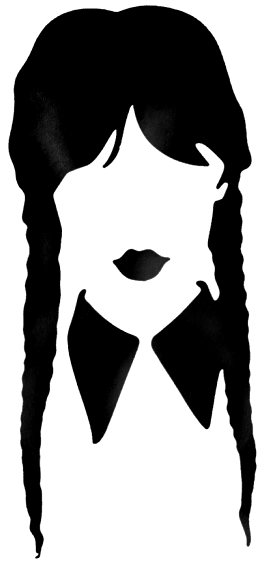
\includegraphics[height=1.35em]{figures/icons/mira-silhouette.png}}{}}}\enspace{\scshape\color{black}Scene}\enspace\textperiodcentered\enspace{\bfseries #1}\pdblockheadingend{\itshape #2}}%
    \end{tcolorbox}\par\addvspace{8pt plus 2pt}%
  }%
  \long\def\xrefbox#1{\par\pd@settle\addvspace{4pt}\noindent\pd@marginhead{See also}{\small #1}\par\addvspace{4pt}}%
  % A generic "Thesis" margin label does not identify which claim matters.
  % Keep the prose; use an authored keyidea head only when it adds meaning.
  \long\def\pdthesis#1{\par\pd@settle\addvspace{6pt plus 1pt}\noindent#1\par\addvspace{6pt plus 1pt}}%
  \long\def\pullquote#1{\pdthesis{#1}}%
}
\makeatother

% Shared visual language for the Book's figures -- version 2.
% Twin: book/figures/pd-figure-language.tex (byte-identical; edit both).
% The standard behind it, the migration from v1 and the QA loop live in
% skills/tikz-diagram-craft/ (SKILL.md, references/figure-standard.md).
%
% This file defines voices, hues, weights and marks -- not layouts.  Every
% figure still chooses a grammar from its reader question.
%
% ===========================================================================
% 1.  THE TYPE LADDER.  Three voices, one size, each tied to a role.
%       pd title   bold      panel titles, row and actor heads, column heads
%       pd label   upright   node text, state names, axis titles, tick words,
%                            relation words on an edge, badge numerals
%       pd note    italic    the one annotation a figure is allowed
%     `pd tag` is the label voice knocked out of the page, for a word that
%     must sit near a rule.  `pd kind` (small caps) is a one- or two-word kind
%     tag, never a title.  Every piece of figure text is mixed case; \texttt
%     only for identifiers that are literally code; math mode for symbols.
%
% 2.  THE COLOUR SYSTEM.  Hue is meaning, and the meanings cross chapters.
%     The figure's own subject is drawn in the CHAPTER hue (`pd focus ...`),
%     resolved from \pdcurrentchaptercolor, which the Book sets per chapter;
%     a fragment declares its standalone fallback with \pdfigurehue{...}.
%     Anything else the figure names takes its concept hue:
%       pd truth       pdcobalt   kernel, truth, the thing being specified
%       pd legible     pdteal     legibility, digest, inspection
%       pd ready       pdhealth   ready, coordinated, admitted, passing
%       pd protocol    pdindigo   protocol, federation, the wire
%       pd identity    pdviolet   identity, continuity, a card, an ID
%       pd reputation  pdrust     reputation, trust earned over time
%       pd value       pdgold     economy, value, settlement, payment
%       pd breach      pderror    breach, refusal, revocation, correction
%       pd warn        pdamber    warning; rules and stripes only, never text
%     Each concept X yields X, X rule, X arrow, X state, X fill, X datum and
%     X label.  Two to four hues a figure; colour is always doubled by shape,
%     dash, weight or a word (breach and warn are dashed as well as coloured).
%
% 3.  THE WEIGHT LADDER.  Exactly three weights, .5 / .9 / 1.6 pt
%     (1 : 1.8 : 3.2).  .5: hairline, guide, tick, artifact edge, fill edge,
%     mark outline, badge.  .9: rule, arrow, state edge, concept arrow.
%     1.6: spine, focus rule, focus and concept state edges, concept rule.
%     A reader sees which line is the subject.  Tips scale with the stroke.
%
% 4.  THE SURFACE LADDER.  pd state (page ground, ink edge) < pd artifact
%     (page ground, grey edge, subordinate) < pd focus state and the concept
%     states (24 % tint, edged in the same hue).  Text is always ink.  A
%     terminal state has a double boundary; an automaton's states are circles
%     (`pd automaton state/focus/terminal`); a ledger's pools are buckets
%     joined by pipes (`pd bucket`, `pd pipe`); a trust boundary is a dashed
%     rectangle (`pd trust boundary`).
%
% 5.  THE GROUND.  Body pages print on white, so every knockout and every
%     neutral surface is `pdpage` (white), never cream: a cream backing on a
%     white page reads as a sticker, which is what v1's figures were covered
%     in.  Neutral regions (Gantt bands, wells) are a warm grey tint.
%
% 6.  EDITIONS.  The Book sets \pdedition (maritime | swiss | technical) and
%     figures/pd-figure-language-<edition>.tex restyles the same names, so one
%     drawing renders in each edition's character.  A fragment that names a
%     raw colour (hhteal, pdcobalt!40, blue) bypasses this; name a role.
% ===========================================================================
% Libraries every v2 mark needs (diamonds, braces, markings), and
% pgfplots for computed plots. This file is \input in every preamble (the
% Book's and each standalone chapter's), so a plot works in all of them.
\usetikzlibrary{arrows.meta,matrix,patterns.meta,positioning,calc,fit,
  backgrounds,shapes.geometric,shapes.multipart,shapes.misc,decorations.pathreplacing,
  decorations.markings,quotes,intersections}
\RequirePackage{pgfplots}
\pgfplotsset{compat=1.18}
\usepgfplotslibrary{fillbetween,groupplots}

\colorlet{pdpage}{white}

% --- the chapter hue, resolved late --------------------------------------
% \pdfigurehue{pdindigo} on the line before a tikzpicture names the hue the
% figure is drawn in when it is compiled outside the Book (a standalone
% chapter, or the skill's renderer).  Inside the Book the preamble has already
% defined \pdcurrentchaptercolor and the chapter opener sets it, so there the
% opener wins and \providecommand does nothing.  Local to the figure's group.
\newcommand{\pdfigfraghue}{pdcobalt}
\newcommand{\pdfigurehue}[1]{%
  \renewcommand{\pdfigfraghue}{#1}%
  \providecommand{\pdcurrentchaptercolor}{#1}}
\newcommand{\pdsetfocushue}{%
  \ifdefined\pdcurrentchaptercolor
    \colorlet{pdfocus}{\pdcurrentchaptercolor}%
  \else
    \colorlet{pdfocus}{\pdfigfraghue}%
  \fi}
\colorlet{pdfocus}{pdcobalt}

% ===========================================================================
% THE TYPOGRAPHIC LAW
% ===========================================================================
% Companion to the line-weight law in figures/pd-palette.tex (1px texture,
% 1.5px linework, 2px enclosure). Same shape of rule: name the roles, fix the
% values, one place.
%
% ONE SIZE. Every named text role in a figure is \pdfiglabelsize
% (= \footnotesize). Roles separate by WEIGHT, SLOPE, FAMILY and INK -- never
% by size. A fragment never writes a size command of its own; if a distinction
% needs making, it takes the role that makes it.
%
% Where the size comes from. Measured, not chosen:
%   \tiny  \scriptsize  \footnotesize  \small  \normalsize
%   5.23    6.97          8.72           9.55    10.46  pt   Book (10.5pt
%                                                            Pagella, 4.5in
%                                                            column, 7x10in)
%   5.98    7.97          8.97           9.96    10.91  pt   standalone chapter
%                                                            (11pt Latin Modern)
% \scriptsize renders at 6.97pt in the Book -- under figcheck's 7pt T1 floor
% before a single width promotion, so it is illegal by measurement, not taste.
% \footnotesize holds 8.72pt and still clears the floor at the 0.85 \resizebox
% limit craft-rules sets (7.41pt). It is also what the corpus already voted
% for: 78 of the 91 local font= declarations this law replaces were already
% \footnotesize, \footnotesize\bfseries or \footnotesize\itshape.
%
% \pdfigbasesize (= \small) is the tikzpicture's ambient size only, so an
% unstyled node is never SMALLER than a styled one; every named role steps
% down exactly one notch from it and none steps down twice.
%
% ONE FACE, AND IT IS THE DOCUMENT'S. \pdfiglabelfamily is empty by default,
% which means figure type inherits whatever face the document is setting --
% Palatino in the Book, Computer Modern in a standalone chapter. Figures
% agreeing with EACH OTHER is not the goal; figures agreeing with the
% paragraph beside them is. A fragment therefore never names a family. Not
% \sffamily (which resolves to Latin Modern Sans against a Computer Modern
% page and reads as a foreign object on it), not \rmfamily, not
% \fontfamily{...}. P18 in tikz_precheck.py is an error for exactly that.
% An edition MAY substitute a face -- the Swiss and technical editions set
% \pdfiglabelfamily to \pdgrotesk, because grotesk display is their declared
% character -- and it does so in ONE command in ONE file, so the substitution
% is a decision on the record rather than an accident in a fragment. The
% only family a fragment may ask for is the identifier one, and it asks for
% it by role (pd mono label / \pdfiglabelmono), never by \ttfamily.
%
% What the roles are, and what each one is for:
%   pd panel title        bold        the name of a panel
%   pd row label          bold        an actor/row name east of its lane
%   pd reverse row label  bold, cream a row name sitting on a dark band
%   pd axis label         regular     an axis title or a tick numeral
%   pd direct label       regular     a value or name riding its own mark
%   pd reverse label      regular, cream  a direct label on a dark band
%   pd mono label         mono        an identifier, path, or literal
%   pd verdict            bold        a terminal outcome stamp (CLEAR, REJECT)
%   pd note               italic      one aside per figure
%   pd legend             regular     a pgfplots legend entry
%   pd state / terminal / actor / artifact / decision   node text
%   pd axis               the whole pgfplots typographic block, one key
%   \pdfigsub             a gloss line under a heading INSIDE a node
%   \pdfigmath            math carrying a sub/superscript, inside a label
%
% A fragment that needs a compound style of its own composes it from a role
% above (`gate/.style={pd decision,minimum width=2cm}`), or, where no role
% fits, from the \pdfiglabel* handles here. It never writes a raw size
% command: P16 in skills/harbor-chartwork/scripts/tikz_precheck.py is an
% error for exactly that, and P10/P11 have been errors for \tiny and
% \scriptsize since before this law.
%
% What does NOT transfer from the screen rules these roles otherwise follow.
% The dataviz method those rules come from assumes an interactive chart: a
% tooltip carries any value a label could not fit, a filter row rescopes the
% view, hover lifts the hovered mark. A printed page has none of that, and the
% absence is not a defect to design around. The INTENT of the tooltip rule --
% "every value is reachable without gating" -- does transfer, and on this page
% it is discharged somewhere else: the value is in the caption, in the margin
% apparatus, or in the chapter's own worked example. So a label that will not
% fit inside its mark moves outside the mark or is dropped to the caption; it
% is never shrunk to fit, because there is no size below \footnotesize to shrink
% to, and never clipped. Do not add a hover affordance, a legend toggle, or a
% filter to a figure in this book.
%
% IDENTIFIERS GET ONE SPELLING. A key, a cell id, a file name or any other
% literal a reader could type is set in `pd mono label` (or \pdfiglabelmono
% inside a compound style), spelled exactly as the code spells it: sk_A, not
% skA and not sk with a subscript A; card0, not card-nought and not a Unicode
% subscript zero. A figure that shows the same identifier two ways has told
% the reader they are two things. The subscripted form belongs to MATHEMATICS
% ($\kappa_7$, an index into a sequence) and the literal form to CODE -- one
% figure may use both, for different objects, but never both for the same
% one. (A precheck for two spellings of one identifier inside a fragment is
% being added on another branch; this is the convention it will enforce.)
%
% SHAPE IS A CHANNEL, AND IT HAS TO SURVIVE THE PRINT SIZE. pd datum, pd
% focus datum and pd caution datum carry three different forms, because the
% house palette is three low-chroma print inks and every distinction it makes
% has to be doubled by something that is not colour. That only counts if the
% form is still legible at 2.1-2.7 pt: an edition that flattens all three to
% one form has removed the second channel and left the figure separating its
% classes by hue alone, which fails in greyscale and for a colour-blind
% reader. Any edition override that restyles a datum must keep three
% distinguishable forms, and must be checked on a render at 1.0x, not
% reasoned about from the point sizes.
%
% One screen rule that does NOT bind here, and why. "Text never wears the data
% colour" exists because a light categorical hue is illegible as text on a
% light surface. The house figure hues are print inks, not screen hues --
% hhink #1B1712, hhteal #00564C, hhamber #6B4500 -- and all three clear text
% contrast on cream, so a label MAY wear its series' ink to bind itself to a
% curve, which is direct labelling and saves a legend. The rule that survives
% is the reason behind it: text wears one of those three inks at full
% strength, or hhink!80!hhgray for recessive furniture, and nothing else. A
% tint of an ink (text=hhgray, text=hhteal!60) is not a role; it is a fade.
% ===========================================================================

\providecommand{\pdfiglabelfamily}{}            % an edition may set \pdgrotesk
\providecommand{\pdfiglabelsize}{\footnotesize} % every named text role
\providecommand{\pdfigbasesize}{\small}         % the picture's ambient size
\providecommand{\pdfiglabel}{\pdfiglabelfamily\pdfiglabelsize}
\providecommand{\pdfiglabelbold}{\pdfiglabel\bfseries}
\providecommand{\pdfiglabelitalic}{\pdfiglabel\itshape}
\providecommand{\pdfiglabelmono}{\pdfiglabelsize\ttfamily}
% The one role that is not a node style, because it lives INSIDE a node's text:
% the second line under a heading that glosses it ("reviewer role / obligation +
% capability + authority"). Every fragment that needed it reached for \tiny or
% \scriptsize, which is how seven \tiny and twelve \scriptsize survived P10/P11
% as hard errors in the corpus. It steps down by SLOPE and WEIGHT, not size, so
% it stays legible and stays legal, and it touches neither family nor ink --
% which is what lets it sit on a reversed node without vanishing.
\providecommand{\pdfigsub}{\mdseries\itshape}
% The one place the law's own size is not the right size.
%
% Measured, both preambles, on a subscripted label inside `pd direct label`:
%
%              base glyph   subscript   subscript as % of base
%   chapter      8.97pt       5.98pt            66.7%
%   Book         8.72pt       6.36pt            72.9%
%   promoted    10.91/10.46   7.97/7.64
%
% An earlier version of this comment said those subscripts are "under figcheck's
% 7pt T1 floor". They are not, and the correction is worth more than the claim
% was. T1 has TWO bands: running text is held to 7.0pt, and a span of three
% glyphs or fewer -- a sub/superscript, a tick numeral -- is held to 5.9pt
% (T1_SHORT_SPAN_PT). That second band is not a loophole. A subscript is set at
% roughly 70% of its base by every typesetter that has ever existed; holding one
% to the running-text floor would mean either no subscripts in figures at all,
% or a figure whose base type is 10pt against 8.72pt body text.
%
% So \pdfigmath is NOT a T1 remedy, and using it as one is how a rule gets
% applied where it does not belong. It exists because 5.98pt clears the
% short-span band by 0.08pt, and 0.08pt is not a margin: a font substitution, an
% edition that nudges \pdfigbasesize, or a chapter that loads a different math
% font puts that subscript under the band with nobody having decided anything.
% Promotion puts it at 7.97/7.64pt -- over even the running-text floor -- while
% the base glyph stays close enough to its neighbours that the label still reads
% as one label.
%
% Use it ONLY for a math group that carries a sub- or superscript. Plain math
% takes the label's own size like any other text, and P22 in tikz_precheck.py is
% an error if it does not.
\providecommand{\pdfigmath}{\normalsize}

% ---------------------------------------------------------------------------
% THE GUIDE DASH, IN ABSOLUTE POINTS, IN ONE PLACE.
%
% `pd guide` used to read `line width=.45pt,densely dotted`. `densely dotted`
% expands to `dash pattern=on \pgflinewidth off 1pt`, and \pgflinewidth is read
% when the KEY is processed, not when the path is stroked. So the Swiss
% edition's `pd guide/.append style={draw=hhink!40,line width=.5pt}` widened the
% stroke and left the dash at the .45pt already baked into it. The canonical
% Book therefore shipped a 0.448pt dot on a 0.498pt stroke.
%
% MEASURED IN THE SHIPPED ARTIFACT, not in a probe: 50 guide strokes sampled
% pixel by pixel in the committed coordination-papers-mega-volume.pdf, at 150
% dpi / 1.0x.
%
%   on 0.448pt = 0.93 device px -- UNDER ONE PIXEL; off 0.996pt = 2.08 px
%   the dash DECLARES 69% of each line's length as gap
%   only 34% of each line's pixels actually reach paper
%   35.4% of three-period windows contain NO pixel that reaches paper at all
%
% That last number is the defect. The gap (2.08 px) is narrower than the
% antialias spread of a 0.93 px stroke, so as the pattern's phase drifts along a
% line the gaps fill in: over a third of every guide's length there is no gap
% left and it is a continuous grey stroke, while the rest of the same line still
% reads as dots. The ink arrives. The DOTTEDNESS does not. A reader sees one
% line that is dotted here and solid there, and no author chose that.
%
% Twenty-five of the corpus's thirty-six guide draws use dottedness to mean
% "this line is not a drawn edge", so twenty-five of them were making a
% distinction the page does not carry.
%
% After, same measurement, same probe geometry, Book preamble:
%   on 1.2pt = 2.50 px, off 2.0pt = 4.17 px, stroke .7pt = 1.45 px
%   0.0% of three-period windows are without paper -- every gap survives,
%     at every phase
%   50% of pixels reach paper against 62.5% declared, the shortfall now being
%     the stroke's antialias skirt rather than the whole signal
%
% ON THE INK, because the obvious reading of this change is wrong. The BASE pair
% was never the problem: hhgray!62 against the hairline's hhgray!78 is 0.411
% against 0.517 of nominal ink, well apart. The problem is that the Book renders
% the SWISS edition (\pdedition defaults to swiss; the committed Book PDF is
% full of hhink!40 guides), where the pair was hhink!40 against hhink!45 -- 4.6%
% of the grey scale. Deleting the Swiss override, which is the right fix for the
% geometry, makes the base ink govern the Book too -- and hhgray!62 is 0.411
% against the Book hairline's 0.410. The same grey, to a thousandth. So the base
% ink has to move, or the dash would go back to carrying the whole distinction
% by itself, which is how this started.
%
% hhink!70 measured against the hairline, mean ink on the page at 150 dpi:
%   chapter  guide 0.0502  hairline 0.0790   guide is 64% of the hairline
%   Book     guide 0.0545  hairline 0.0671   guide is 81% of the hairline
% Per DOT it is 0.638 against 0.410 -- unmistakably a different mark. In MEAN it
% is still lighter than the hairline -- so it still recedes. Two channels, both
% working, instead of one that does not.
%
% The replacement is stated absolutely and measures phase-STABLE: every dot
% renders at the same weight wherever it falls on the grid (peak column ink
% 0.808, invariant across twelve sub-pixel offsets). It is a macro rather than
% three numbers because an edition that restates one of them and not the others
% is how this defect happened. The geometry is a LEGIBILITY FLOOR, not an
% edition's character: an edition may move the guide's ink, and states the
% geometry through these two macros so it cannot half-restate it.
%
% Any dash in this corpus is stated in absolute points. The `dotted` family
% (`dotted`, `densely dotted`, `loosely dotted`) derives its on-length from the
% line width and is therefore banned -- P23 in tikz_precheck.py. `dashed` and
% its relatives are absolute (on 3pt off 3pt) and are fine.
\providecommand{\pdguidewidth}{.7pt}
% Three lengths, not one macro holding the whole key: pgfkeys splits a key list
% on `,` and `=` before expanding anything (so a macro carrying `dash
% pattern=...` is read as one key NAME), and TikZ's dash-pattern scanner reads
% the literal words `on`/`off` without expanding a macro that hides them. A
% dimension after each word does expand, which is the seam that works.
\providecommand{\pdguideon}{1.2pt}
\providecommand{\pdguideoff}{2.0pt}

\tikzset{
  % --- picture level: one size, one default tip, the chapter hue -----------
  % A figure label is a name, not prose: it never hyphenates.
  pd figure/.style={font=\pdfiglabelfamily\pdfigbasesize,text=pdink,line cap=round,line join=round,
    >={Stealth[length=2.6pt 3.2,width=2.0pt 2.4]},/utils/exec=\pdsetfocushue,
    every node/.append style={execute at begin node={%
      \hyphenpenalty=10000\exhyphenpenalty=10000\relax}}},
%
  % --- 1. the voices ---------------------------------------------------------
  pd title/.style={font=\pdfiglabelbold,text=pdink,align=center},
  pd label/.style={font=\pdfiglabel,text=pdink,align=center},
  pd note/.style={font=\pdfiglabelitalic,text=pdinkmuted,align=left},
  pd kind/.style={font=\pdfiglabel\scshape,text=pdinkmuted,align=center},
  pd tag/.style={pd label,fill=pdpage,inner sep=1.7pt},
%
  % --- 4. surfaces -----------------------------------------------------------
  pd state/.style={pd label,draw=pdink,line width=.9pt,fill=pdpage,
    rounded corners=1pt,inner xsep=6pt,inner ysep=4.5pt,minimum height=7.4mm},
  % a terminal state carries a double boundary, as every automaton text draws it
  pd terminal/.style={pd state,double=pdpage,double distance=1.1pt,line width=.5pt},
  pd artifact/.style={pd label,draw=pdinkmuted!60,line width=.5pt,fill=pdpage,
    rounded corners=1pt,inner xsep=5pt,inner ysep=3.5pt,minimum height=6.2mm},
  pd panel/.style={draw=pdinkmuted!55,line width=.5pt,
    dash pattern=on 2.4pt off 2pt,rounded corners=2.5pt,inner sep=7pt,align=center},
  pd hatch/.style={pattern={Lines[angle=45,distance=4pt,line width=.3pt]},
    pattern color=pdinkmuted!70},
  pd neutral fill/.style={fill=pdinkmuted!12,draw=pdinkmuted!55,line width=.5pt},
%
  % --- 3. strokes ------------------------------------------------------------
  pd hairline/.style={draw=pdinkmuted!45,line width=.5pt},
  % Absolute dash, from the typographic law's three macros above: a guide is a
  % definite dotted construction line, darker per dot than the hairline and
  % lighter in mean ink. A lattice is the quiet continuous grid a figure stands on.
  pd guide/.style={draw=pdink!70,line width=\pdguidewidth,dash pattern=on \pdguideon off \pdguideoff},
  pd lattice/.style={draw=pdinkmuted!40,line width=.4pt},
  pd tick/.style={draw=pdinkmuted!75,line width=.5pt},
  pd rule/.style={draw=pdink,line width=.9pt},
  pd spine/.style={draw=pdink,line width=1.6pt},
  pd thin arrow/.style={draw=pdinkmuted!75,line width=.5pt,->},
  pd arrow/.style={pd rule,->},
  pd spine arrow/.style={pd spine,->},
%
  % --- the chapter hue, as the figure's focus --------------------------------
  pd focus rule/.style={draw=pdfocus,line width=1.6pt},
  pd focus arrow/.style={pd focus rule,->},
  pd focus state/.style={pd state,draw=pdfocus,line width=1.6pt,fill=pdfocus!24},
  % The single solid chapter-colour surface in a figure: use only for the
  % culmination or object the reader should name after five seconds. Editions
  % may render ordinary focus with a pale field while keeping this one solid.
  pd climax state/.style={pd focus state},
  % a member of the subject's set when the set, not one node, is the subject:
  % edged in the chapter hue, never filled, so the one solid node stays unique
  pd focus outline/.style={pd state,draw=pdfocus,line width=1.2pt,fill=pdpage},
  pd focus fill/.style={fill=pdfocus!24,draw=pdfocus,line width=.5pt},
  pd focus datum/.style={circle,fill=pdfocus,draw=pdpage,line width=.5pt,inner sep=2.6pt},
  pd focus label/.style={pd label,text=pdfocus!85!pdink},
%
  % --- marks -----------------------------------------------------------------
  pd datum/.style={circle,fill=pdink,draw=pdpage,line width=.5pt,inner sep=2.3pt},
  pd badge/.style={pd label,circle,draw=pdink,line width=.5pt,fill=pdpage,
    inner sep=.5pt,minimum size=5.0mm},
  pd focus badge/.style={pd badge,draw=pdfocus,line width=.9pt,fill=pdfocus!24},
  % --- conventions shared by every chapter (Critical Analysis, 2026-09-08) ---
  % Automata: states are circles, terminal (accepting) states double circles;
  % edge words are short action names; guards go in an aligned legend table.
  pd automaton state/.style={pd label,circle,draw=pdink,line width=.9pt,fill=pdpage,
    minimum size=11mm,inner sep=1pt},
  pd automaton focus/.style={pd automaton state,draw=pdfocus,line width=1.6pt,fill=pdfocus!24},
  pd automaton terminal/.style={pd automaton state,double=pdpage,double distance=1.1pt,
    line width=.5pt},
  pd initial/.style={draw=pdink,line width=.9pt,->},
  % Ledgers: asset pools are rectangular buckets (open at the top) joined by
  % directed pipes; the conserved sum is set as an equation under the rails.
  pd bucket/.style={pd label,draw=none,minimum width=2.2cm,minimum height=1.3cm,
    append after command={\pgfextra{\draw[draw=pdink,line width=.9pt]
      (\tikzlastnode.north west) -- (\tikzlastnode.south west)
      -- (\tikzlastnode.south east) -- (\tikzlastnode.north east);}}},
  pd pipe/.style={draw=pdink,line width=.9pt,double=pdpage,double distance=2.2pt,
    -{Stealth[length=3.4pt 2,width=5.2pt]}},
  pd focus pipe/.style={pd pipe,draw=pdfocus},
  % Trust boundaries: a dashed rectangle is the Dolev-Yao interface; a vector
  % that escapes it is drawn in pd breach and named.
  pd trust boundary/.style={draw=pdink,line width=.9pt,dash pattern=on 4pt off 2.4pt,
    rounded corners=0pt,inner sep=8pt},
  % a stroke that ends at a badge is shortened, so no rule touches the numeral
  pd to badge/.style={shorten >=2pt},
  pd from badge/.style={shorten <=2pt},
}

% ===========================================================================
% 7.  PLOTS.  A plot is computed by a committed script, never sketched.  `pd
%     axis` is the one axis grammar: two spines (left, bottom), ticks out, no
%     box, no grid unless asked (`pd grid`), tick words in the label voice,
%     numbers with a thin-space thousands separator, room outside the plot for
%     direct labels (clip=false).  Series are named at their ends, not in a
%     legend: `pd series` (ink), `pd focus series` (chapter hue), and
%     `pd X series` for a concept; breach and warn series are dashed.  A
%     region between curves is `pd focus fill`/`X fill` with fillbetween.
%     Width: `width=` is the plot box (scale only axis); leave about 1.6 cm
%     of the 11.4 cm column for the y tick words and title.
% ===========================================================================
\pgfplotsset{
  pd axis/.style={
    scale only axis,width=8.8cm,height=4.6cm,
    axis lines*=left,axis line style={draw=pdink,line width=.5pt,-},
    tick align=outside,major tick length=3pt,minor tick length=0pt,
    tick style={draw=pdink,line width=.5pt},
    tick label style={pd label,text=pdinkmuted},
    label style={pd label},title style={pd title},
    every axis title/.append style={yshift=-2pt},
    enlargelimits=false,clip=false,
    grid=none,
    legend style={draw=none,fill=none,font=\pdfiglabel},
    /pgf/number format/1000 sep={\,},
    every axis plot/.append style={line width=.9pt,line join=round,mark size=1.7pt},
  },
  pd grid/.style={ymajorgrids,major grid style={draw=pdinkmuted!30,line width=.4pt}},
  pd series/.style={draw=pdink,mark=*,mark options={fill=pdink,draw=pdpage,line width=.5pt,solid}},
  pd focus series/.style={draw=pdfocus,line width=1.6pt,mark=*,
    mark options={fill=pdfocus,draw=pdpage,line width=.5pt,solid}},
  pd muted series/.style={draw=pdinkmuted!70,line width=.9pt,mark=none},
}
\newcommand{\pdplotconcept}[2]{%
  \pgfplotsset{#1 series/.style={draw=#2,mark=*,
    mark options={fill=#2,draw=pdpage,line width=.5pt,solid}}}}
\pdplotconcept{pd truth}{pdcobalt}
\pdplotconcept{pd legible}{pdteal}
\pdplotconcept{pd ready}{pdhealth}
\pdplotconcept{pd protocol}{pdindigo}
\pdplotconcept{pd identity}{pdviolet}
\pdplotconcept{pd reputation}{pdrust}
\pdplotconcept{pd value}{pdgold}
\pgfplotsset{
  pd breach series/.style={draw=pderror,dash pattern=on 3.2pt off 2.2pt,mark=diamond*,
    mark options={fill=pderror,draw=pdpage,line width=.5pt,solid}},
  pd warn series/.style={draw=pdamber,dash pattern=on 3.2pt off 2.2pt,mark=none},
}

% ===========================================================================
% Supplied visual-guide primitives: native Book type, deliberate strokes,
% readable Stealth heads, open markers, and a quiet quantitative grid.
% These are opt-in: old diagrams need spacing review before thicker arrows.
\tikzset{
  pd guide step/.style={pd artifact,draw=pdink,fill=pdpage,line width=1pt,
    align=center,minimum height=40pt,inner xsep=5pt,inner ysep=6pt},
  pd guide arrow/.style={draw=pdcobalt,line width=1.15pt,
    -{Stealth[length=7pt,width=4.4pt]},shorten <=2pt,shorten >=2pt},
}
\newcommand{\pdflowstep}[4]{%
  \node[pd guide step,text width=#4] (#1) at #2 {#3};}
\newcommand{\pdflowlink}[2]{%
  \draw[pd guide arrow] (#1.east)--(#2.west);}
\pgfplotsset{
  pd evidence axis/.style={pd axis,
    axis line style={draw=pdink,line width=1pt,-},
    tick style={draw=pdink,line width=.8pt},
    grid=major,major grid style={draw=pdinkmuted!20,line width=.35pt},
    axis background/.style={fill=pdpage}},
  pd evidence measured/.style={draw=pdcobalt,line width=1.35pt,mark=*,
    mark size=2.6pt,mark options={fill=pdpage,draw=pdcobalt,line width=1.1pt}},
  pd evidence comparison/.style={draw=pdink,line width=1.1pt,
    dash pattern=on 4pt off 2.5pt,mark=square*,mark size=2.2pt,
    mark options={fill=pdink,draw=pdink,solid}},
}
% Analytic curves, not sampled observations. Integer samples preserve the
% meaning of reviewer count; callers set axes and name their assumptions.
\newcommand{\pdindependentmisses}[2]{%
  \addplot[pd evidence measured,domain=1:#2,samples=#2] {100*(1-#1)^x};}
\newcommand{\pdreviewcost}[1]{%
  \addplot[pd evidence measured,domain=1:#1,samples=#1] {x};}
% 8.  UML.  The Book's engineering diagrams use UML 2.5 notation, so a reader
%     who knows UML reads them without a key.  Four kinds:
%     STATE MACHINE  `pd uml state` (rounded), `pd uml focus state`, a
%       composite drawn with `pd uml composite` around its substates plus a
%       compartment of internal transitions; `pd uml initial` (filled dot),
%       `pd uml final` (bullseye), `pd uml choice` (diamond); transitions are
%       `pd uml transition` (open arrowhead) labelled  event [guard] / effect.
%     SEQUENCE  `pd uml head` (lifeline head), `pd uml lifeline` (dashed),
%       `pd uml activation` (thin bar), messages `pd uml sync` (filled head),
%       `pd uml async` (open head), `pd uml reply` (dashed, open head),
%       `pd uml fragment` + `pd uml fragment tag` for alt / opt / loop.
%     COMPONENT  `pd uml component` with \pdumlicon{node} (the component
%       glyph) and a <<component>> keyword; `pd uml port`; provided interface
%       \pdumlprovided{from}{to}{name} (lollipop), required \pdumlrequired (socket).
%     ERD (crow's foot)  `pd er entity` (rectangle split: name, then rows;
%       mark keys PK / FK in the row text), relationship lines `pd er rel`
%       with tips `er one`, `er many`, `er zero or one`, `er one or many`,
%       `er zero or many` at either end.
% ===========================================================================
\pgfdeclarearrow{
  name = pd crow,
  parameters = {\the\pgfarrowlength,\the\pgfarrowwidth},
  setup code = {%
    \pgfarrowssettipend{0pt}%
    \pgfarrowssetlineend{0pt}%
    \pgfarrowssetbackend{-\pgfarrowlength}%
    \pgfarrowsupperhullpoint{0pt}{.5\pgfarrowwidth}%
    \pgfarrowsupperhullpoint{-\pgfarrowlength}{0pt}%
    \pgfarrowssavethe\pgfarrowlength
    \pgfarrowssavethe\pgfarrowwidth},
  drawing code = {%
    \pgfsetdash{}{0pt}%
    \pgfpathmoveto{\pgfqpoint{-\pgfarrowlength}{0pt}}%
    \pgfpathlineto{\pgfqpoint{0pt}{.5\pgfarrowwidth}}%
    \pgfpathmoveto{\pgfqpoint{-\pgfarrowlength}{0pt}}%
    \pgfpathlineto{\pgfqpoint{0pt}{-.5\pgfarrowwidth}}%
    \pgfusepathqstroke},
  defaults = {length=2.4mm, width=3.0mm}
}
\tikzset{
  % state machine
  pd uml state/.style={pd state,rounded corners=4.5pt},
  pd uml focus state/.style={pd focus state,rounded corners=4.5pt},
  pd uml terminal/.style={pd terminal,rounded corners=4.5pt},
  pd uml composite/.style={draw=pdink,line width=.9pt,rounded corners=7pt,fill=none,inner sep=0pt},
  pd uml initial/.style={circle,fill=pdink,draw=none,minimum size=2.4mm,inner sep=0pt},
  pd uml final/.style={circle,draw=pdink,line width=.9pt,fill=pdpage,minimum size=3.6mm,inner sep=0pt,
    path picture={\fill[pdink] (path picture bounding box.center) circle (1.1mm);}},
  pd uml choice/.style={diamond,draw=pdink,line width=.9pt,fill=pdpage,minimum size=4.2mm,inner sep=0pt},
  pd uml transition/.style={pd rule,-{Straight Barb[length=2.2pt 2.2,width=4.4pt 2.2]}},
  pd uml focus transition/.style={pd focus rule,-{Straight Barb[length=2.2pt 2.2,width=4.4pt 2.2]}},
  pd uml breach transition/.style={pd rule,draw=pderror,dash pattern=on 3.2pt off 2.2pt,
    -{Straight Barb[length=2.2pt 2.2,width=4.4pt 2.2]}},
  % sequence
  pd uml head/.style={pd state,rounded corners=0pt,minimum height=6.8mm},
  pd uml lifeline/.style={draw=pdinkmuted!75,line width=.5pt,dash pattern=on 3pt off 2pt},
  pd uml activation/.style={draw=pdink,line width=.5pt,fill=pdpage,minimum width=2.2mm,inner sep=0pt},
  pd uml sync/.style={pd rule,-{Triangle[length=3.2pt 1.6,width=3.2pt 1.6]}},
  pd uml async/.style={pd rule,-{Straight Barb[length=2.4pt 2,width=4.4pt 2]}},
  pd uml reply/.style={pd rule,dash pattern=on 3pt off 2pt,-{Straight Barb[length=2.4pt 2,width=4.4pt 2]}},
  pd uml fragment/.style={draw=pdink,line width=.5pt,fill=none,inner sep=6pt},
  pd uml fragment tag/.style={pd label,font=\footnotesize\bfseries,draw=pdink,line width=.5pt,fill=pdpage,
    inner xsep=3pt,inner ysep=2pt,chamfered rectangle,chamfered rectangle corners=south east,
    chamfered rectangle xsep=2pt},
  % component
  pd uml component/.style={pd state,rounded corners=0pt,align=center,inner xsep=8pt,inner ysep=6pt,minimum height=11mm},
  pd uml port/.style={rectangle,draw=pdink,line width=.5pt,fill=pdpage,minimum size=2mm,inner sep=0pt},
  % ERD
  pd er entity/.style={pd label,rectangle split,rectangle split parts=2,rectangle split part align={center,left},
    draw=pdink,line width=.9pt,fill=pdpage,inner xsep=5pt,inner ysep=3pt,align=left,
    rectangle split part fill={pdinkmuted!12,pdpage}},
  pd er rel/.style={pd rule},
  er one/.tip={Bar[width=3.0mm,sep=1.2pt]Bar[width=3.0mm]},
  er many/.tip={Bar[width=3.0mm,sep=1.4pt]pd crow},
  er zero or one/.tip={Circle[open,length=1.8mm,width=1.8mm,sep=1.2pt,fill=pdpage]Bar[width=3.0mm]},
  er one or many/.tip={Bar[width=3.0mm,sep=1.4pt]pd crow},
  er zero or many/.tip={Circle[open,length=1.8mm,width=1.8mm,sep=1.2pt,fill=pdpage]pd crow},
}
% the component glyph, drawn in the top-right corner of a component node
\newcommand{\pdumlicon}[1]{%
  \begin{scope}[shift={($(#1.north east)+(-4.2mm,-2.6mm)$)},x=1mm,y=1mm]
    \draw[pdink,line width=.5pt,fill=pdpage] (0,-1.1) rectangle (2.6,1.1);
    \draw[pdink,line width=.5pt,fill=pdpage] (-.6,.25) rectangle (.6,.65);
    \draw[pdink,line width=.5pt,fill=pdpage] (-.6,-.65) rectangle (.6,-.25);
  \end{scope}}
% a provided interface (lollipop) from a node side to a point, with its name
\newcommand{\pdumlprovided}[3]{%
  \draw[pd rule] (#1) -- (#2);
  \draw[pd rule,fill=pdpage] (#2) circle (1.3mm);
  \node[pd label,anchor=south] at ($(#2)+(0,1.6mm)$) {#3};}
% a required interface (socket): a half-circle open toward the provider
\newcommand{\pdumlrequired}[4]{% from, to, name, facing angle of the socket's opening
  \draw[pd rule] (#1) -- (#2);
  \draw[pd rule] ($(#2)+(#4+90:1.9mm)$) arc[start angle=#4+90,end angle=#4+270,radius=1.9mm];
  \node[pd label,anchor=north] at ($(#2)+(0,-2.4mm)$) {#3};}

% --- 2. the concept map, as styles, so a drawing never chooses a hue --------
% An edition file may \renewcommand\pdconcept before the map below expands.
\newcommand{\pdconcept}[2]{%
  \tikzset{%
    #1/.style={draw=#2,text=pdink},
    #1 rule/.style={draw=#2,line width=1.6pt},
    #1 arrow/.style={draw=#2,line width=.9pt,->},
    #1 state/.style={pd state,draw=#2,line width=1.6pt,fill=#2!24},
    #1 fill/.style={fill=#2!24,draw=#2,line width=.5pt},
    #1 datum/.style={circle,fill=#2,draw=pdpage,line width=.5pt,inner sep=2.6pt},
    #1 label/.style={pd label,text=#2!85!pdink},
  }}

% --- 6. the edition layer, loaded before the concept map expands ----------
\ifdefined\pdedition\IfFileExists{figures/pd-figure-language-\pdedition.tex}{\input{figures/pd-figure-language-\pdedition}}{}\fi

\pdconcept{pd truth}{pdcobalt}
\pdconcept{pd legible}{pdteal}
\pdconcept{pd ready}{pdhealth}
\pdconcept{pd protocol}{pdindigo}
\pdconcept{pd identity}{pdviolet}
\pdconcept{pd reputation}{pdrust}
\pdconcept{pd value}{pdgold}
\pdconcept{pd breach}{pderror}
\pdconcept{pd warn}{pdamber}
% Breach and warning read as refusals, so they are dashed as well as
% coloured, and a breach mark is a diamond where every other mark is a circle.
% Amber is never text (3.71:1 on white); a warn label is set in ink.
\tikzset{
  pd breach rule/.append style={dash pattern=on 3.2pt off 2.2pt},
  pd breach arrow/.append style={dash pattern=on 3.2pt off 2.2pt},
  pd warn rule/.append style={dash pattern=on 3.2pt off 2.2pt},
  pd warn arrow/.append style={dash pattern=on 3.2pt off 2.2pt},
  pd breach datum/.append style={diamond},
  pd warn label/.style={pd label},
}

% ===========================================================================
% v1 NAMES.  Kept so every existing fragment still compiles; they resolve to
% the v2 roles, so an untouched figure inherits the ladder.  New work uses the
% v2 names (skills/tikz-diagram-craft/references/migration-v1-to-v2.md).
% ===========================================================================
\tikzset{
  pd row label/.style={pd title,anchor=east},
  pd panel title/.style={pd title,align=left},
  pd axis label/.style={pd label},
  % Direct labels sit beside their mark; they do not erase a line or box
  % underneath themselves. A label that needs a paper knockout is misplaced
  % and must be moved, not given an invisible patch.
  pd direct label/.style={pd tag,fill=none,align=left},
  pd actor/.style={pd state},
  pd boundary/.style={pd panel},
  pd caution rule/.style={pd breach rule},
  pd caution arrow/.style={pd breach arrow},
  pd caution fill/.style={pd breach fill},
  pd caution datum/.style={pd breach datum},
}

% ===========================================================================
% Roles named on main by the typographic law (#10191), expressed on the v2
% roles so an edition's .append style on the parent reaches them. `pd danger`
% is main's name for what v2 calls `pd breach` (red, dashed, diamond marks);
% both names resolve to one family. Main's hairline-boxed fact badge is
% `pd fact badge`: v2's `pd badge` is the numbered guard/step marker.
% ===========================================================================
\tikzset{
  pd danger rule/.style={pd breach rule},
  pd danger arrow/.style={pd breach arrow},
  pd danger fill/.style={pd breach fill,text=pdink},
  pd danger datum/.style={pd breach datum},
  pd ink fill/.style={fill=pdink,draw=pdink,line width=.4pt,text=pdpage},
  pd decision/.style={pd state,diamond,aspect=1.55,font=\pdfiglabelbold,
    minimum height=0pt,inner xsep=3pt,inner ysep=3pt},
  pd mono label/.style={pd direct label,font=\pdfiglabelmono,inner xsep=2.5pt,inner ysep=2.5pt},
  pd verdict/.style={pd direct label,font=\pdfiglabelbold},
  pd reverse label/.style={pd direct label,text=pdpage,fill=none},
  pd reverse row label/.style={pd row label,text=pdpage},
  pd legend/.style={font=\pdfiglabel,text=pdink,draw=none,fill=none},
  pd kind tag/.style={pd kind,align=right},
  pd fact badge/.style={pd hairline,font=\pdfiglabel,text=pdink,align=center,
    inner sep=2.4pt,fill=none},
}

% Small reusable marks.  They deliberately avoid prose-bearing boxes.
\newcommand{\pdfigaxis}[4]{%
  \draw[pd rule,->] (#1,#2) -- (#3,#2);
  \node[pd label,anchor=west] at (#3,#2) {#4};
}
\newcommand{\pdfigvaxis}[4]{%
  \draw[pd rule,->] (#1,#2) -- (#1,#3);
  \node[pd label,anchor=south] at (#1,#3) {#4};
}

% Native-size, object-based evidence figures; shared by Book and chapters.
% Shared approved Swiss evidence drawing primitives. Keep both chapter roots identical.
\ifdefined\pdSwissEvidenceLoaded\else
\def\pdSwissEvidenceLoaded{1}
% Real ink-box gate; no declared coordinate envelope can substitute for this.
\newsavebox{\sgEvidenceBox}
\newcommand{\SGMeasuredFigure}[2]{%
  \sbox{\sgEvidenceBox}{#2}%
  \typeout{SG-GEOMETRY: #1,width=\the\wd\sgEvidenceBox,height=\the\dimexpr\ht\sgEvidenceBox+\dp\sgEvidenceBox\relax}%
  \ifdim\wd\sgEvidenceBox>325.215pt
    \PackageError{swiss-evidence}{Figure #1 exceeds the Book column}{Recompose at native text size; do not scale.}%
  \fi
  \usebox{\sgEvidenceBox}}
% Parent redraws after rejection of lab specimens 01,04,06.
% All coordinates are physical TeX points; no resizebox or transformed fonts.
\usetikzlibrary{arrows.meta,calc}
% Aliased onto the house palette (figures/pd-palette.tex), not \definecolor'd
% as independent HTML values: an edition that restyles pdcobalt/pdteal/...
% now restyles every SG figure with it. The six values were already
% bit-identical matches for pdcobalt/pdteal/pdviolet/pdamber/pderror/pdink;
% the alias turns that into a guarantee instead of a coincidence.
\colorlet{sgBlue}{pdcobalt}
\colorlet{sgTeal}{pdteal}
\colorlet{sgViolet}{pdviolet}
\colorlet{sgAmber}{pdamber}
\colorlet{sgRed}{pderror}
\colorlet{sgInk}{pdink}
\definecolor{sgGrid}{HTML}{D8C7A6}
% The one house size, inheriting the document's own face (the typographic
% law in pd-figure-language.tex): no \sffamily leak, no local \fontsize.
\newcommand{\SGType}{\pdfiglabel}
\tikzset{sg/base/.style={x=1pt,y=1pt,line cap=butt,line join=miter,
  every node/.style={font=\SGType,inner sep=0pt,text=sgInk}},
  sg/arrow/.style={-{Stealth[length=4.5pt,width=3.6pt]},draw=sgInk,line width=.85pt},
  sg/grid/.style={draw=sgGrid,line width=.3pt},
  sg/hash/.style={draw=sgBlue,fill=sgBlue!7,line width=1pt,minimum width=53pt,
    minimum height=27pt,inner sep=4pt,align=center},
  sg/sibling/.style={draw=sgAmber,fill=sgAmber!10,line width=1pt,minimum width=51pt,
    minimum height=27pt,inner sep=4pt,align=center},
  sg/check/.style={draw=sgInk,fill=white,line width=1pt,minimum width=92pt,
    minimum height=30pt,inner sep=5pt,align=center}}

% A folded record, not an undifferentiated rounded node. Width/height are pt.
\newcommand{\SGDocument}[6]{%
  \begin{scope}[shift={#2}]
    \path[draw=sgInk,fill=#5,line width=.85pt]
      (0,0)--({#3-7},0)--(#3,7)--(#3,#4)--(0,#4)--cycle;
    \draw[sgInk,line width=.65pt] ({#3-7},0)--({#3-7},7)--(#3,7);
    \node[minimum width=#3pt,minimum height=#4pt,text width=\dimexpr#3pt-12pt\relax,
      align=center] (#1) at ({#3/2},{#4/2}) {#6};
  \end{scope}}

\newcommand{\SGSurvival}{%
\begin{tikzpicture}[sg/base]
  % Three complete probability decades, percentages rather than tiny exponents.
  \foreach \x in {0,1,...,6}{\draw[sg/grid] ({35+30*\x},20)--({35+30*\x},140);}
  \foreach \y/\lab in {20/{0.1\%},60/{1\%},100/{10\%},140/{100\%}}{%
    \draw[sg/grid] (35,\y)--(215,\y);
    \draw[sgInk,line width=.65pt] (32,\y)--(35,\y);
    \node[anchor=east] at (28,\y) {\lab};}
  \draw[sgInk,line width=.85pt] (35,140)--(35,20)--(215,20);
  \foreach \x in {0,2,4,6}{%
    \draw[sgInk,line width=.65pt] ({35+30*\x},20)--({35+30*\x},17);
    \node[anchor=north] at ({35+30*\x},12) {$\x$};}
  \node[rotate=90] at (-9,80) {jobs still running (log scale)};
  \node[anchor=north] at (125,-5) {duration / mean duration};
  \draw[sgBlue,line width=1.5pt,domain=0:6,samples=100]
    plot ({35+30*\x},{140-120*ln(1+\x/2)/ln(10)});
  \draw[sgViolet,line width=1.2pt,dash pattern=on 4pt off 2.5pt,domain=0:6,samples=100]
    plot ({35+30*\x},{140-40*\x/ln(10)});
  % Endpoint leaders have allocated space; text does not lie on a curve.
  \draw[sgBlue,line width=.8pt] (215,67.75)--(224,67.75);
  \node[anchor=west,text=sgBlue,font=\SGType\bfseries] at (230,73) {Lomax};
  \node[anchor=west,text=sgBlue] at (230,60) {1.56\%};
  \draw[sgViolet,line width=.8pt,dashed] (215,35.77)--(224,35.77);
  \node[anchor=west,text=sgViolet,font=\SGType\bfseries] at (230,40) {exponential};
  \node[anchor=west,text=sgViolet] at (230,27) {0.248\%};
\end{tikzpicture}}

\newcommand{\SGTiming}{%
\begin{tikzpicture}[sg/base,y=-1pt]
  % This bracket spans COMMIT TO SYNC. It is not a range of hypothetical syncs.
  \path[draw=sgAmber!35,fill=sgAmber!9,line width=.5pt] (39,19) rectangle (253,49);
  \draw[sgAmber,line width=1pt] (39,18)--(39,9)--(253,9)--(253,18);
  \node[anchor=south,text=sgAmber,font=\SGType\bfseries] at (146,5) {?};
  \draw[sgInk,line width=.9pt] (39,27)--(39,45) (253,27)--(253,45);
  \draw[{Stealth[length=4.5pt,width=3.6pt]}-{Stealth[length=4.5pt,width=3.6pt]},
    sgAmber,line width=1.3pt] (40,36)--(252,36);
  \node[anchor=north,font=\SGType\bfseries] at (39,52) {commit};
  \node[anchor=north,font=\SGType\bfseries] at (253,52) {WAL sync};
  \node[anchor=west] at (0,86) {heartbeats received};
  \foreach \x/\label in {57/{s_1},117/{s_2},194/{s_3},278/{s_4}}{%
    \draw[sgViolet!70,dashed,line width=.55pt] (\x,104)--(\x,145);
    \node[anchor=south,text=sgViolet] at (\x,101) {$\label$};}
  \path[draw=sgAmber!35,fill=sgAmber!9,line width=.5pt] (158,108) rectangle (243,142);
  \draw[sg/grid] (0,139)--(306,139);
  \draw[sgTeal,line width=1.4pt]
    (0,132)--(25,132)--(25,116)--(33,116)--(33,132)
    --(85,132)--(85,116)--(93,116)--(93,132)
    --(145,132)--(145,116)--(153,116)--(153,132)--(306,132);
  \draw[sgRed,line width=1pt] (243,106)--(243,145);
  \node[anchor=north,text=sgRed] at (243,149) {deadline};
  \draw[sg/arrow] (0,174)--(306,174);
  \node[anchor=north east] at (306,179) {time};
\end{tikzpicture}}

\newcommand{\SGInclusion}{%
\begin{tikzpicture}[sg/base,y=-1pt]
  % Two independent inputs: a supplied proof and an issuer-authenticated root.
  \node[anchor=north west,font=\SGType\bfseries,text width=158pt,align=left] at (0,0)
    {Recompute from the receipt};
  \node[anchor=north west,font=\SGType\bfseries,text width=118pt,align=left] at (193,0)
    {Authenticate\\the checkpoint};
  \draw[sg/grid,step=15pt] (0,29) grid (175,194);
  \SGDocument{receipt}{(4,35)}{49}{34}{sgViolet!9}{receipt $P$}
  \node[sg/hash] (leaf) at (29,103) {$a=H_L(P)$};
  \node[sg/sibling] (sibone) at (108,103) {sibling $b$};
  \node[sg/hash] (inner) at (68,146) {$u=H_N(a,b)$};
  \node[sg/sibling] (sibtwo) at (146,146) {subtree $c$};
  \node[sg/hash,fill=sgBlue,text=white,minimum width=100pt] (computed) at (107,190)
    {$R'=H_N(u,c)$};
  \draw[sg/arrow,draw=sgViolet] (receipt.south)--(leaf.north);
  \draw[sg/arrow,draw=sgBlue] (leaf.south)--(inner.north west);
  \draw[sg/arrow,draw=sgAmber] (sibone.south)--(inner.north east);
  \draw[sg/arrow,draw=sgBlue] (inner.south)--(computed.north west);
  \draw[sg/arrow,draw=sgAmber] (sibtwo.south)--(computed.north east);
  \SGDocument{checkpoint}{(211,37)}{85}{48}{sgTeal!8}{signed root $R^*$\\size $n=4$\\signature $\sigma$}
  % The trusted key is an external input, not something the prover supplies.
  \draw[sgInk,line width=1pt] (218,113) circle (3.5pt);
  \draw[sgInk,line width=1pt] (221.5,113)--(233,113) (230,113)--(230,117) (233,113)--(233,117);
  \node[anchor=west] at (239,113) {trusted $pk_I$};
  \node[sg/check,minimum width=84pt] (verify) at (260,158) {verify $\sigma$\\result $A$};
  \draw[sg/arrow,draw=sgTeal] (checkpoint.east)--(311,61)--(311,158)--(verify.east);
  \draw[sg/arrow] (247,123)--(247,138)--(verify.north);
  \node[sg/check,minimum width=112pt,minimum height=34pt] (compare) at (164,245)
    {$A\ \land\ (R'=R^*)$};
  \draw[sg/arrow,draw=sgBlue] (computed.south)--(107,220)--(compare.north west);
  \draw[sg/arrow,draw=sgTeal] (verify.south)--(260,214)--(compare.north east);
  \node[anchor=east,text=sgTeal] at (250,204) {$R^*,A$};
  \node[draw=sgTeal,fill=sgTeal,text=white,minimum width=90pt,
    minimum height=27pt,font=\SGType\bfseries] (accept) at (76,299) {accept inclusion};
  \node[draw=sgRed,fill=white,text=sgRed,line width=1.2pt,minimum width=90pt,
    minimum height=27pt,font=\SGType\bfseries] (reject) at (256,299) {reject proof};
  \draw[sg/arrow,draw=sgTeal] (compare.south west)--(108,279)--(76,279)--(accept.north);
  \draw[sg/arrow,draw=sgRed] (compare.south east)--(220,279)--(256,279)--(reject.north);
  \node[anchor=south,text=sgTeal] at (82,275) {true};
  \node[anchor=south,text=sgRed] at (248,275) {false};
\end{tikzpicture}}

% Reusable geometry; load after swiss-redraws.tex. Real points, no scaling.
\newcommand{\SGDatabase}[4]{%
  \begin{scope}[shift={#2}]
    \path[draw=#3,fill=#3!7,line width=.9pt]
      (0,4)--(0,32) arc[start angle=180,end angle=360,x radius=24pt,y radius=5pt]
      --(48,4) arc[start angle=0,end angle=-180,x radius=24pt,y radius=5pt];
    \draw[draw=#3,fill=#3!7,line width=.9pt] (24,4) ellipse[x radius=24pt,y radius=5pt];
    \node[minimum width=48pt,minimum height=37pt,align=center] (#1) at (24,18) {#4};
  \end{scope}}

% Reader question: How do overlapping requests become ordered records?
% Evidence: schematic two-client history, not a runtime observation.
% Each request precedes commit 1; each reply follows its own committed record.
\newcommand{\SGWriterSequence}{%
\begin{tikzpicture}[sg/base,y=-1pt]
  % Recomposed at native size: a 22-character mono request label no longer
  % fits a 118pt lane gap at \pdfiglabelmono, so the HTTP verb is shortened
  % to the identifier it names and the resource it names ("auth.ts") moves
  % to the lane header, where it reads once instead of twice.
  \foreach \x/\lanelabel in {35/{{\pdfigmath$\alpha_{\text{auth}}$} (claude)},153/{Kernel (single writer)},275/{{\pdfigmath$\alpha_{\text{bill}}$} (codex)}}{
    \node[anchor=south,font=\pdfiglabelbold,align=center] at (\x,0) {\lanelabel};
    \draw[sg/grid] (\x,9)--(\x,237);}
  % Both invocations precede the first commit: overlapping client requests.
  \draw[sg/arrow,draw=sgViolet] (35,29)--(153,29);
  \node[anchor=south,text=sgViolet,font=\pdfiglabelmono] at (94,24) {POST /claims};
  \draw[sg/arrow,draw=sgAmber] (275,57)--(153,57);
  \node[anchor=south,text=sgAmber,font=\pdfiglabelmono] at (214,52) {POST /claims};
  % commit 1 succeeds: drawn in the kernel's own hue. commit 2 is the
  % kernel's WAL record of a REFUSAL, not a second grant -- it is drawn in
  % the breach hue so the outcome is doubled by colour, not stated in prose
  % alone (the typographic law's "colour is always doubled" rule). The
  % "lock held" highlight band is gone: at native size it ran directly
  % behind this text, which figcheck reads as a drawn line through the
  % words, and the sequencing arrows already carry the serialization claim.
  \SGDocument{commitA}{(93,71)}{120}{46}{sgBlue!8}{{\pdfiglabelbold commit 1 \textperiodcentered{} WAL 4102}\\[2pt]{\pdfigsub {\pdfigmath$\alpha_{\text{auth}}$} \textperiodcentered{} epoch 104}}
  \draw[sg/arrow,draw=sgViolet,dash pattern=on 3pt off 2pt] (153,130)--(35,130);
  \node[anchor=south,text=sgViolet,font=\pdfiglabel] at (94,128) {201 Created};
  \SGDocument{commitB}{(93,152)}{120}{46}{sgRed!8}{{\pdfiglabelbold commit 2 \textperiodcentered{} WAL 4103}\\[2pt]{\pdfigsub {\pdfigmath$\alpha_{\text{bill}}$} refused}}
  \draw[sg/arrow,draw=sgAmber,dash pattern=on 3pt off 2pt] (153,213)--(275,213);
  \node[anchor=south,text=sgAmber,font=\pdfiglabel] at (214,211) {409 Conflict};
  \draw[sg/arrow] (3,20)--(3,232);
  \node[anchor=west,font=\pdfiglabel] at (9,236) {time};
\end{tikzpicture}}

% Reader question: What is checked before the service admits requests?
% Source: SQLite WAL documentation, sections 2--2.2, cited in the chapter.
% Checkpointing copies committed pages; it does not apply uncommitted work.
% The dashed group denotes separate mechanisms, not a proved composition.
\newcommand{\SGRecoveryAdmission}{%
\begin{tikzpicture}[sg/base,y=-1pt]
  % Recomposed at native size: a 25-character mono command (sqlite3_wal_
  % checkpoint_v2) no longer fits a 103pt-wide column once the label grows
  % from 5.0pt to \pdfiglabelmono, so the three mechanisms read top to
  % bottom, full measure, instead of left to right in three narrow lanes.
  \draw[sgInk!55,dash pattern=on 3pt off 2pt,line width=.7pt]
    (0,0) rectangle (300,318);

  % 1. Checkpoint WAL
  \node[anchor=north west,align=left,text width=228pt] at (10,8)
    {{\pdfiglabelbold 1. Checkpoint WAL}\\[2pt]
     {\pdfiglabelmono\color{sgBlue} sqlite3\_wal\_checkpoint\_v2}\\[2pt]
     {\pdfigsub Copies committed WAL pages into the main database; uncommitted frames are not applied.}};
  \SGDocument{walback}{(247,4)}{34}{26}{sgViolet!7}{}
  \SGDocument{walfront}{(253,9)}{34}{26}{sgViolet!7}{WAL}
  \draw[sg/arrow] (18,101)--(18,118);

  % 2. Check Pages
  \node[anchor=north west,align=left,text width=228pt] at (10,122)
    {{\pdfiglabelbold 2. Check Pages}\\[2pt]
     {\pdfiglabelmono\color{sgTeal} PRAGMA integrity\_check}\\[2pt]
     {\pdfigsub Verifies B-tree pointers and freelist allocation across every page.}};
  \SGDatabase{db}{(251,118)}{sgBlue}{SQLite}
  \draw[sg/arrow] (18,215)--(18,232);

  % 3. Verify Links
  \node[anchor=north west,align=left,text width=228pt] at (10,236)
    {{\pdfiglabelbold 3. Verify Links}\\[2pt]
     {\pdfiglabelmono\color{sgAmber} Merkle chain verify}\\[2pt]
     {\pdfigsub Validates cryptographic audit-log continuity link by link.}};
  \foreach \x in {249,267,285}{
    \draw[sgAmber,line width=1pt,rounded corners=2pt] (\x,240) rectangle ({\x+14},256);}
  \draw[sgAmber,line width=1pt] (259,248)--(267,248) (281,248)--(289,248);

  % Decision Gate
  \node[sg/check,minimum width=165pt,minimum height=28pt,font=\pdfiglabelbold] (admit) at (150,350)
    {all critical checks pass?};
  \draw[sg/arrow] (150,318)--(admit.north);

  \node[draw=sgTeal,fill=sgTeal,text=white,minimum width=125pt,minimum height=32pt,
    align=center] (serve) at (65,420) {{\pdfiglabelbold admit requests}\\[1.5pt]{\pdfigsub HTTP 200 Ready (:9876)}};
  \node[draw=sgRed,fill=white,text=sgRed,line width=1pt,minimum width=125pt,
    minimum height=32pt,align=center] (refuse) at (235,420) {{\pdfiglabelbold refuse service}\\[1.5pt]{\pdfigsub HTTP 503 Unavailable}};

  \draw[sg/arrow,draw=sgTeal] (admit.south west)--(90,384)--(65,384)--(serve.north);
  \draw[sg/arrow,draw=sgRed] (admit.south east)--(210,384)--(235,384)--(refuse.north);
  % Each tag sits clear of its own diagonal leg, on the side the diagonal
  % does NOT occupy -- PASS left of its bend, FAIL right of its bend --
  % rather than centred on the bend where the stroke crosses the glyphs.
  \node[anchor=south east,text=sgTeal,font=\pdfiglabelbold] at (63,382) {PASS};
  \node[anchor=south west,text=sgRed,font=\pdfiglabelbold] at (237,382) {FAIL (HALT)};
\end{tikzpicture}}

% Named bands and their audiences; the dashed floor is NOT a fifth layer.
\newcommand{\SGStackLayers}{%
\begin{tikzpicture}[sg/base,y=-1pt]
  \foreach \y/\level/\name/\audience/\evidence/\hue in {
    0/3/Economy/{Between operators}/{settlement and reputation}/sgAmber,
    51/2/Legibility/{For the operator}/{summaries linked to evidence}/sgTeal,
    102/1/Coordination/{Between agents}/{permissions and commitments}/sgViolet,
    153/0/Substrate/{On one machine}/{ordered writes and records}/sgBlue}{
    \path[draw=\hue,fill=\hue!8,line width=1pt] (17,\y) rectangle (142,{\y+38});
    \node[anchor=west,font=\SGType\bfseries,text=\hue] at (26,{\y+13}) {L\level};
    \node[anchor=west,font=\SGType\bfseries] at (26,{\y+27}) {\name};
    \node[anchor=north west,font=\SGType\bfseries] at (158,{\y+2}) {\audience};
    \node[anchor=north west,text width=149pt,align=left] at (158,{\y+17}) {\evidence};}
  \foreach \y in {153,102,51}{\draw[sg/arrow] (79,\y)--(79,{\y-13});}
  \draw[sgBlue,line width=2.4pt] (7,154)--(7,190);
  \draw[sgInk!60,dashed,line width=.7pt] (17,204) rectangle (307,243);
  \node[anchor=west,font=\SGType\bfseries] at (26,216) {Machine floor};
  \node[anchor=west] at (26,231) {file lock, clock, socket, supervisor};
  \draw[sg/arrow] (79,204)--(79,192);
\end{tikzpicture}}

% Compact counterpart for future chapter-by-chapter marginal navigation.
% A named current-layer argument changes emphasis, never the layer order.
\newcommand{\SGMarginLadder}[1]{%
\begin{tikzpicture}[sg/base,y=-1pt]
  \foreach \y/\n/\name/\hue in {0/3/Economy/sgAmber,37/2/Legibility/sgTeal,74/1/Coordination/sgViolet,111/0/Substrate/sgBlue}{
    \draw[\hue,line width=.7pt] (0,\y)--(91,\y);
    \node[anchor=north west,text=\hue,font=\SGType\bfseries] at (4,{\y+3}) {L\n};
    \node[anchor=north west] at (4,{\y+16}) {\name};
    \ifnum\n=#1\relax\draw[\hue,line width=2pt] (0,{\y+3})--(0,{\y+29});\fi}
\end{tikzpicture}}

\fi



% ─── Maturity markers (self-grading of every claim) ────────────────────
% \Built, \BuiltWeak, \Designed and \Vision, and the \Closed/\Partial/\Open
% proof-obligation markers of the open-problem and status tables, are defined
% once, for this paper and for the Book, in figures/pd-pedagogy.tex (\input
% above).

% ─── Pull-quote sidebar: large quote, left-edge accent stripe. ────────────────
\newcommand{\pullquote}[1]{%
  \par\vspace{6pt}%
  \noindent\begin{tikzpicture}
    \node[draw=none,fill=hhsand!22,line width=0pt,
          inner sep=10pt,text width=\dimexpr\textwidth-30pt\relax,
          align=left] (q) {%
      \itshape\large #1%
    };
    \draw[hhcobalt,line width=2.5pt] (q.north west) -- (q.south west);
  \end{tikzpicture}\par\vspace{6pt}%
}

% ─── Teaching callouts: \keyidea{} and \pitfall{} (the pedagogic idiom) ────────
% Quiet: thin left rule + subtle sand fill, small-caps muted-ink label.
\newcommand{\keyidea}[1]{%
  \par\vspace{6pt}%
  \noindent\begin{tikzpicture}
    \node[draw=none,fill=hhsand!18,rounded corners=2pt,
          inner sep=8pt,text width=\dimexpr\textwidth-24pt\relax,align=left] (k) {%
      \small{\scshape\bfseries\textcolor{hhgray}{Key idea.}}\enspace #1%
    };
    \draw[hhgray!60,line width=1pt] (k.north west) -- (k.south west);
  \end{tikzpicture}\par\vspace{6pt}%
}
% Pitfall accents its LABEL only.
\newcommand{\pitfall}[1]{%
  \par\vspace{6pt}%
  \noindent\begin{tikzpicture}
    \node[draw=none,fill=hhsand!18,rounded corners=2pt,
          inner sep=8pt,text width=\dimexpr\textwidth-24pt\relax,align=left] (p) {%
      \small{\scshape\bfseries\textcolor{hhcobalt}{Pitfall.}}\enspace #1%
    };
    \draw[hhgray!60,line width=1pt] (p.north west) -- (p.south west);
  \end{tikzpicture}\par\vspace{6pt}%
}

% ─── Companion-paper / cross-reference box ────────────────────────────────────
\newcommand{\xrefbox}[1]{%
  \vspace{4pt}\noindent\begin{tikzpicture}
  \node[draw=hhgray!45,line width=0.4pt,fill=hhsand!18,rounded corners=2pt,
        inner sep=8pt,text width=\dimexpr\textwidth-22pt\relax,align=left]{%
    \small #1};
  \end{tikzpicture}\vspace{4pt}%
}

% ─── Listings Setup ──────────────────────────────────────────────────────────
\lstdefinestyle{pseudocode}{
  backgroundcolor=\color{codebg},
  frame=single,
  rulecolor=\color{codeframe},
  basicstyle=\ttfamily\small,
  keywordstyle=\color{hhink}\bfseries,
  commentstyle=\color{hhgray}\itshape,
  stringstyle=\color{hhgray},
  numbers=left,
  numberstyle=\tiny\color{gray},
  numbersep=8pt,
  breaklines=true,
  showstringspaces=false,
  tabsize=2,
  xleftmargin=15pt,
  xrightmargin=5pt,
  framexleftmargin=15pt,
  captionpos=b
}
\lstset{style=pseudocode}

% ─── Theorem Environments ─────────────────────────────────────────────────────
\theoremstyle{definition}
\newtheorem{definition}{Definition}[section]
\newtheorem{theorem}{Theorem}[section]
\newtheorem{lemma}{Lemma}[section]
\newtheorem{proposition}{Proposition}[section]
\newtheorem{property}{Property}[section]
\newtheorem{corollary}{Corollary}[section]
\newtheorem{conjecture}{Conjecture}[section]

\theoremstyle{definition}
\newtheorem{protocol}{Protocol}[section]

\theoremstyle{remark}
\newtheorem*{remark}{Remark}

% ─── Header/Footer ────────────────────────────────────────────────────────────
\pagestyle{fancy}
\fancyhf{}
\fancyhead[L]{\small\itshape\color{hhgray} The Harbor Economy}
\fancyhead[R]{\small\color{hhgray}\thepage}
\fancyfoot[C]{\footnotesize\color{hhgray} Port Daddy Coordination Papers \textperiodcentered\ Chapter~\pdchapternumber\ of \pdchaptercount}
\renewcommand{\headrulewidth}{0.4pt}
\renewcommand{\footrulewidth}{0pt}

% ─── Title ────────────────────────────────────────────────────────────────────
\title{
  \vspace{-1cm}
  {\Large\textsc{Port Daddy Coordination Papers --- Chapter~\pdchapternumber\ of \pdchaptercount}}\\[
0.5cm]
  \rule{\textwidth}{0.5pt}\\[0.3cm]
  {\LARGE\textbf{The Harbor Economy:}}\\[0.2cm]
  {\Large Labor, Rental, and Licensing,\\
   Settling on One Conserving Bond Ledger}\\[0.3cm]
  \rule{\textwidth}{0.5pt}
}
\author{
  \textbf{Erich Owens}\\[0.2cm]
  Curiositech LLC\\[0.2cm]
  \texttt{engineering@portdaddy.dev}
}
\date{\pdeditiondate\\Version 1.3 (textbook edition)}
% ═══════════════════════════════════════════════════════════════════════════════
% Hyperlink and cross-reference discipline (must stay last in the preamble).
% Shared hyperlink and cross-reference discipline for the Book and its chapters.
% Load this LAST in every preamble: cleveref must follow hyperref and amsthm.
% hyperref itself is loaded earlier with [backref=page] (a load-time option).
% Twin copy under book/figures/ (byte-identical; checked by
% scripts/generate-mega-whitepaper.test.mjs).
%
% What a reader gets: live links on chapter titles, section numbers, theorems,
% figures, tables, equations, page numbers, and citations; PDF bookmarks three
% levels deep; and, at the end of every bibliography entry, the pages that cite it.
% Links are quiet: a warm dark ink one step lighter than body text, so the
% four part hues keep their meaning and an inline chapter title never competes
% with the part it sits in. Chrome pages (the front-matter map, part openers)
% recolor their own links locally.
\hypersetup{
  colorlinks=true,
  linkcolor=pdinkmuted,
  citecolor=pdinkmuted,
  urlcolor=pdinkmuted,
  filecolor=pdinkmuted,
  anchorcolor=pdink,
  bookmarksnumbered=true,
  bookmarksdepth=3,
  bookmarksopen=true,
  bookmarksopenlevel=1,
  breaklinks=true,
  linktoc=all,
  pdfauthor={Erich Owens},
  pdftitle={\pdchaptertitle},
  pdfsubject={\pdeditiontitle: \pdeditionsubtitle},
}

% Title-based chapter references. \pdchaplink{prefix}{text} is a live link to
% the chapter inside the Book (the Book's preamble defines it before loading this
% file); in a standalone chapter it is plain text. Prose uses \pdchapref, which
% sets the title in italics; the locator map uses \pdchaplink directly.
\providecommand{\pdchaplink}[2]{#2}
\DeclareRobustCommand{\pdchapref}[2]{\pdchaplink{#1}{\emph{#2}}}

% \ifpdbook -- true in the assembled Book, false otherwise.
%
% WHY THIS EXISTED. A drawing that two chapters both \input prints twice in the
% Book, under two figure numbers. The fix is for the chapter that develops the
% idea to keep the figure and the other to point at it -- but the standalone
% edition of a chapter had nowhere to point, and rewriting the prose outright
% removed five figures from harbor-economy-whitepaper.pdf and left it telling a
% conference reader that a ceremony is "drawn in The Federated Harbor", a
% document that reader did not have.
%
% WHERE IT STANDS NOW. The per-chapter PDFs are retired: the Book is the one
% document, so \ifpdbook is true in every build that renders, and the \else
% branches are source with no output. They are still here, and still read by
% check_duplicate_figures.py (which must not count an \else \input as a Book
% input) -- but nothing prints them, and nothing new should be put in one.
% Whether to delete them is an open question; see the retirement PR.
%
% The divergence was per-build. A CONDITIONAL and not a two-argument macro:
% the generator inlines each \input, so a figure branch is a whole table or
% tikzpicture, and as a macro argument that is scanned as one token list --
% which is how \pdinbook produced "runaway argument" on the first attempt.
% \ifpdbook skips the untaken branch at the TeX level instead.
%
% Declared unconditionally and defaulting FALSE, which is the standalone
% answer. The Book's preamble sets \pdbooktrue immediately after loading
% this file. A guard here would have to mention \ifpdbook or \newif inside a
% branch TeX may skip, and a conditional token in skipped text is counted as
% a nested \if -- which is how two attempts at a guard both produced
% "Incomplete \ifdefined". Ordering is cheaper than cleverness.
\newif\ifpdbook

% cleveref: "Theorem 3.1", "Figure 2.4", "Section 1.3", capitalised, never
% abbreviated, with the whole phrase clickable. Names are declared explicitly
% because the theorem environments are created before this file is loaded.
\usepackage[nameinlink,capitalise,noabbrev]{cleveref}
\crefname{pdchapter}{Chapter}{Chapters}
\crefname{part}{Part}{Parts}
\crefname{appendix}{Appendix}{Appendices}
\crefname{definition}{Definition}{Definitions}
\crefname{theorem}{Theorem}{Theorems}
\crefname{lemma}{Lemma}{Lemmas}
\crefname{proposition}{Proposition}{Propositions}
\crefname{corollary}{Corollary}{Corollaries}
\crefname{conjecture}{Conjecture}{Conjectures}
\crefname{property}{Property}{Properties}
\crefname{protocol}{Protocol}{Protocols}
\crefname{lsprotocol}{Protocol}{Protocols}
\crefname{stpprotocol}{Protocol}{Protocols}
\crefname{heprotocol}{Protocol}{Protocols}
\crefname{remark}{Remark}{Remarks}
\crefname{lstlisting}{Listing}{Listings}
\crefname{exercise}{Exercise}{Exercises}
\crefname{solution}{Solution}{Solutions}
\Crefname{pdchapter}{Chapter}{Chapters}
\Crefname{lstlisting}{Listing}{Listings}
\Crefname{exercise}{Exercise}{Exercises}
\Crefname{solution}{Solution}{Solutions}

% Back-references: "^ Cited on pages 12, 40, and 87." after every bibliography
% entry, each page number a live link back to the page that cited the work.
% Distinct pages only (#3/#4).
%
% The page numbers used to be wrapped in \color{hhgray} along with the words,
% which painted over the link colour hyperref had just given them: the links
% were there -- 29 annotations on a typical bibliography page -- and looked
% exactly like the grey prose around them, so nobody knew they could click.
% Restoring the quiet link colour would not have fixed it either; pdinkmuted
% against hhgray is 1.53:1, which is no signal at footnote size.
%
% So the numbers take pdcobalt (7.55:1 on the cream, and a hue a reader cannot
% mistake for grey), and the line opens with the return arrow this book already
% uses to send a solution back to its exercise. This is a deliberate exception
% to the quiet-link discipline above, and the reason is that back-matter
% navigation is the one place where the link IS the content: in prose the
% surrounding sentence tells you a phrase is a destination, and in a
% bibliography nothing does.
\renewcommand*{\backref}[1]{}
\renewcommand*{\backrefalt}[4]{%
  \ifcase #3\relax
  \or {\footnotesize{\color{hhgray}$\uparrow$~Cited on page}~{\hypersetup{linkcolor=pdcobalt}#4}{\color{hhgray}.}}%
  \else {\footnotesize{\color{hhgray}$\uparrow$~Cited on pages}~{\hypersetup{linkcolor=pdcobalt}#4}{\color{hhgray}.}}%
  \fi}
\renewcommand*{\backrefsep}{, }
\renewcommand*{\backreftwosep}{ and }
\renewcommand*{\backreflastsep}{, and }

\begin{document}
\pdopensolutions
\setlength{\emergencystretch}{2em}
\maketitle
\thispagestyle{empty}
\vspace{0.6cm}
\vspace{0.4cm}
\noindent\textbf{Keywords:} mechanism design, multi-sided markets, incentive
compatibility, reputation systems, capability-based security, cross-chain
settlement, applied category theory, federation, Port Daddy
\vspace{0.4cm}
\noindent\textit{Reading time: approximately 45 minutes end-to-end; about 12
minutes for \S\ref{sec:thesis}--\S\ref{sec:three-sides} alone (the market thesis).
This is Chapter~\pdchapternumber{} of \pdbooktitle{}, and it is written cold: no prior platform
knowledge is assumed. It can be read first, but \S\ref{sec:keystone} relies on
\pdchapref{stp}{From Spawn to Person} for identity, while the
cryptographic hop-bound authorization chain is analyzed in
\pdchapref{anchor}{The Anchor Protocol}.}
\vspace{0.5cm}
% ─── Maturity key (in the header region, per house style) ─────────────────────
\noindent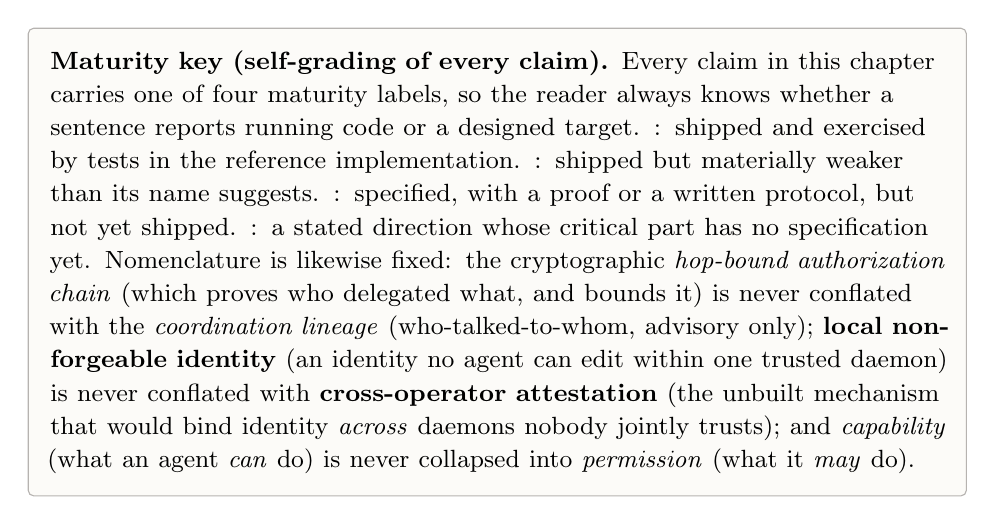
\begin{tikzpicture}
\node[draw=hhgray!45,line width=0.4pt,fill=hhsand!12,rounded corners=2pt,
      inner sep=8pt,text width=\dimexpr\textwidth-22pt\relax,align=left]{%
  \small{\scshape\bfseries Maturity key (self-grading of every claim).}\enspace
  Every claim in this chapter carries one of four maturity labels, so the reader
  always knows whether a sentence reports running code or a designed target.
  \Built{}: shipped and exercised by tests in the reference implementation.
  \BuiltWeak{}: shipped but materially weaker than its name suggests.
  \Designed{}: specified, with a proof or a written protocol, but not yet
  shipped.
  \Vision{}: a stated direction whose critical part has no specification
  yet.
  Nomenclature is likewise fixed: the cryptographic \emph{hop-bound authorization
  chain} (which proves who delegated what, and bounds it) is never conflated with
  the \emph{coordination lineage} (who-talked-to-whom, advisory only);
  \textbf{local non-forgeable identity} (an identity no agent can edit within one
  trusted daemon) is never conflated with \textbf{cross-operator attestation} (the
  unbuilt mechanism that would bind identity \emph{across} daemons nobody jointly trusts);
  and \emph{capability} (what an agent \emph{can} do) is never collapsed into
  \emph{permission} (what it \emph{may} do).%
};
\end{tikzpicture}
\vspace{0.5cm}
\noindent\textbf{Volume Context.} \pdchapref{swk}{The Single-Writer Kernel} is
the local transaction layer and \pdchapref{anchor}{The Anchor Protocol}
proves how its authority delegates; \pdchapref{ls}{The Legible Swarm} is the
operator's front door; \pdchapref{stp}{From Spawn to Person} supplies
continuity and reputation. \emph{This} chapter is the market.
\pdchapref{bonded}{The Bonded Commons} and \pdchapref{fh}{The Federated
Harbor} then prove what the market assumes about settlement and federation.
\newpage
\tableofcontents
\newpage
% ═══════════════════════════════════════════════════════════════════════════════
\section{The thesis: one market for three kinds of trade}\label{sec:thesis}
% ═══════════════════════════════════════════════════════════════════════════════

Bob commissions Alice's team to repair the failing checkout-flow integration
test and refactor the affected payment module. The agreed test must remain;
deleting it is not completion, and an unrelated migration is outside the job.
Alice supplies the team, Dana a profiling lease, and Carol a lint-and-type
skill. These are three promises about one repair, with different payees and
different ways to fail. This is a constructed example; no deployment ran it.

\begin{pdexample}{One repair, two sources of funds}
Bob reserves $400$ credits (\textsc{cr}) for Alice's labor, $50$ for Dana's lease,
and $10$ for Carol's skill licence: $460$ in payment funds. Alice separately
posts $100$ in performance collateral. The contract therefore holds $560$,
not $460$ and not a $560$ bounty.
On a successful repair Carol earns her flat $10$ licence fee, however much
of the repository her skill touched. Alice receives her
$400$ payment and her $100$ collateral back. Returning collateral is not
income.
\end{pdexample}

A float plan is the record of that agreement: the work, the parties,
and the funds each party has committed to it. Bob's reserved money sits in
escrow: the ledger holds it for the contract and releases it only on
the contract's terms. Alice's $100$ is a bond: a deposit she gets back
if she delivers and loses in whole or in part (is \emph{slashed}) if she does
not. The single ledger step at the end, which pays each party from escrow and
returns or slashes each bond, is settlement.
Section~\ref{sec:one-settlement} checks every recipient on both the successful
and partial-completion branches.
Before writing the float plan's formal schema, we ask what Bob buys, who controls the work,
and which evidence authorizes each transfer. We then check conservation, whether the commitments can coexist,
incentives and the obligations that arise when the counterparties have
separate administrators. Each operator's agents run inside a harbor: the
governed environment in which one program, the daemon, checks and records
every change. The local bond ledger is implemented. The rest of the market is
not built: the rental and licensing contracts are designed, while the
reputation estimator and cross-operator attestation still lack a specification
for their critical parts (Appendix~\ref{app:impl}).

\subsection{What the record must identify}
Bob may hire Alice for her past results or rent her Heron specialist, denoted
$a_2$ below. Either reputation-based price needs a history attached to the
actual provider or asset. Carol's licence instead names a skill version by
content hash. Copying that code creates no independent success record.
A prepaid licence for a known hash can trade without reputation; a price
justified by past outcomes needs attributable outcomes. The continuity
requirements of \pdchapref{stp}{From Spawn to Person} therefore become inputs
to pricing, rather than a second definition of personhood.

\pdexercisepointer{\ref{ex:he-clone-word}}{\ref{ex:he-no-identity-market}}{\pageref{ex:he-clone-word}}
% ═══════════════════════════════════════════════════════════════════════════════
\section{Three purchases, three information problems}\label{sec:three-sides}
% ═══════════════════════════════════════════════════════════════════════════════
\paragraph{Three contract choices for the checkout repair.} Bob needs the affected
$1{,}200$-line module refactored. The following labor and rental prices are alternative contract designs, not
additional charges in the $560$ agreement. They isolate who knows what and
who carries the loss.
\emph{Side~1 (labor).} Bob posts a float plan with a $400$\,\textsc{cr} bounty;
Alice takes it as a firm. She dispatches three of her own agents, posts a
$60$\,\textsc{cr} sub-bond per agent ($180$\,\textsc{cr} total), and keeps
$400 - (\text{slashed sub-bonds}) - \text{fee}$. If one of her three agents botches
its slice and is slashed $60$\,\textsc{cr}, Alice absorbs that loss. She carries
her fleet's risk herself, and that is what makes her accountable as a firm.
\emph{Side~2 (capital).} Instead Bob rents Alice's Heron specialist $a_2$ directly for an
afternoon at $90$\,\textsc{cr}. Now there are three parties: Bob (poster), Alice
(owner, privately knows $a_2$'s true quality), and $a_2$ (worker). Bob holds the
runtime control of $a_2$ while it runs on his repository. Under this rental variant Alice's specified exposure is
reputational: if $a_2$ underperforms, $a_2$'s public score falls, and Alice's
asset loses value.
\emph{Side~3 (IP).} Carol never touches Bob's repository at all; she licenses her
lint-and-type skill into Bob's float plan for a flat $10$\,\textsc{cr} fee,
released to Carol \emph{only on green settlement}. Carol is privately informed about
her skill's quality; Bob cannot inspect it before he runs it. One refactor has
three sides, and in each a different party knows something the others do not.
Each of these information problems has a standard name. Labor carries
\emph{moral hazard}, a hidden action: once Alice accepts the bounty, Bob
cannot watch how her fleet works, so the sub-bonds tie her pay to the result.
The rental carries \emph{adverse selection}, a hidden type: Alice knows
$a_2$'s quality before the lease and Bob does not, so $a_2$'s public score is
what Bob can price. The licence sells an \emph{experience good}, whose quality
the buyer learns only by using it. Before use it faces Akerlof's lemons
problem~\pdcite{akerlof1970}, which is why Carol is paid only after the run
settles green.
As the next section shows, all three settle through one escrow.

A \pdterm{two-sided market} (\textbf{Rochet \& Tirole}~\pdcite{rochet2003}, the
foundational reference: \emph{a platform is two-sided when the allocation of the
total price across the two user groups, and not just its level, affects
transaction volume}) is the standard frame for a marketplace: buyers on one side,
sellers on the other, and the platform choosing whom to subsidize so that each
side draws the other in. A simple labor transaction has a \emph{requester} who
posts work and a \emph{worker agent} who does it.
We distinguish three purchases: labor, access to a specialist, and a licence
for a reusable skill. These are contract types; they need not be three disjoint
populations of platform participants. The same operator can buy one and supply
another. Calling a platform two-sided or multi-sided additionally concerns how
participation and pricing on one side affect the others~\pdcite{rochet2006}.
The classification here identifies which private information, rights, and
payments each contract must handle. In the following examples, ``side 1,''
``side 2,'' and ``side 3'' are shorthand for these three contract types. Table~\ref{tab:he-three-purchases}
compares these choices.
\begin{enumerate}[leftmargin=1.6em,itemsep=4pt]
  \item \textbf{Operator-for-hire (labor).} An operator who runs a fleet can sell
    its labor to \emph{another} operator. The operator is now a firm taking
    work-for-hire, with margin $=$ bounty $-\,\Sigma(\text{slashed sub-bonds})\,-$
    ledger fee. Its private information is whether its fleet can deliver. It
    carries its fleet's risk, as a firm is accountable for its employees.
  \item \textbf{Agent/fleet as rentable asset (capital).} An operator who owns a
    well-reputed specialist can \emph{rent it out}. Now the asset-owner, the
    task-poster, and the worker are three different parties with three different
    incentives. The owner's private information is the agent's true quality; its
    exposure is reputational.
  \item \ifpdmargincolumn\pdmarginanalogy{reusable-pattern}{}{ch06-reusable-printing-block}{Like one printing block making many impressions, a licensed skill can be reused without its maker performing each job.}\fi%
    \textbf{Skill/tool as licensed good (IP).} A skill can be \emph{licensed}
    into someone else's float plan, metered or per-use, without the licensor
    doing any task work. The licensor's private information is the skill's quality,
    which the buyer cannot inspect before purchase.
\end{enumerate}
These contracts separate who supplies labor, who controls a rented asset,
and who licenses reusable instructions. If the asset owner is also the task
poster, one counterparty disappears; the rental and labor obligations still
need separate terms.
% Reader question: how does Bob's choice change the seller's exposure?
% The chapter's refactor example, not three abstract risk rails.
% Alternative purchases, not three cumulative charges or paid flows.
% Conservation and reputation subject keys remain in the surrounding prose.
\begin{table}[htbp]
\centering
\begingroup
\pdfiglabelfamily\small
\renewcommand{\arraystretch}{1.2}
\begin{tabularx}{\linewidth}{@{}>{\raggedright\arraybackslash}p{.29\linewidth}@{\hspace{1em}}>{\raggedright\arraybackslash}p{.20\linewidth}@{\hspace{1em}}>{\raggedright\arraybackslash}X@{}}
\toprule
\textbf{Bob buys} & \textbf{Payment} & \textbf{Seller's exposure} \\
\midrule
Work from Alice's three-agent fleet & 400 cr bounty & Alice posts 60 cr per agent; 180 cr in sub-bonds. \\
\addlinespace
An afternoon with Alice's specialist & 90 cr rent & Poor work lowers the specialist's reputation, which is Alice's asset. \\
\addlinespace
Carol's lint-and-type skill & 0.5 cr per file & Carol's fee is released only on successful settlement. \\
\bottomrule
\end{tabularx}
\endgroup
\caption{One refactor, three alternative purchases. Rental and licensing are designed, not shipped; all three use the same escrow. [illustrative]}
\label{tab:he-three-purchases}
\label{fig:he-three-sided}
\end{table}


\ifdefined\pdswisslandmarkplate
\begin{figure}[p]
  \centering
  \pdswisslandmarkplate{09}{\linewidth}
\end{figure}
\pdmarginpagebreak
\fi

\paragraph{When the specialist can fail.} Should Bob rent Alice's specialist
$a_2$, or send the job to a pool of interchangeable agents?
\pdchapref{ls}{The Legible Swarm} answered this for a specialist who never
disappears: the specialist wins when its skill advantage (its service rate
divided by a pool worker's) reaches a threshold $\gamma_A(\rho_{\mathrm{pool}},c)$ that depends on
how busy the pool is ($\rho_{\mathrm{pool}}$) and how many workers it has ($c$). Real
specialists are mortal: sessions die, containers are reaped, providers
leave. So we now add failure and replacement to the model. The specialist
fails at rate $\xi$, and a successor takes over after an $\mathrm{Exp}(\eta)$
spin-up (context transfer, warm-up, credential rebinding). Work resumes where
it stopped (preemptive resume), and requests keep queueing throughout: an
$M/M/1$ queue with breakdowns.

Read the rates before the formula. Requests arrive as a Poisson process at
rate $\lambda>0$ jobs per hour. While available, the specialist serves at
exponential rate $\mu_s>0$ jobs per hour; breakdowns occur at rate $\xi>0$
per available hour, and repair takes mean $1/\eta$ hours, with $\eta>0$.
The clocks are independent. A finite mean wait
requires $\lambda<\mu_s\eta/(\xi+\eta)$: effective capacity must exceed demand.
For example, $\eta=0.25$ means four hours to replace a failed worker;
$\xi=0.5$ means two hours of mean operation between failures. Even an
extremely fast worker then spends two thirds of its time unavailable.

The pool's cost $K$ is measured in hours. It is the pool's mean wait
$W_{\mathrm{pool}}$ plus $A/(w\lambda)$: $K=A/(w\lambda)+W_{\mathrm{pool}}$.
Here $A$ is the hourly value of having one accountable owner; equivalently, it
is the hire-and-monitor overhead that a pool pays and a sole owner avoids.
$w$ is the cost of one hour of delay and $\lambda$ the job arrival rate, so
$A/(w\lambda)$ converts that overhead into an equivalent wait per job. The
ratio $D=\xi/\eta$ below has no units; it is not an amount of credits.
\begin{pdexample}{The Succession Threshold, for a Rented Specialist}
\setlength{\parskip}{4pt plus 1pt}
Side~2 rests on a quiet assumption: that Alice's well-reputed specialist $a_2$ is
worth being a \emph{sole} specialist for, rather than one interchangeable member
of a pool. The specialization boundary settles exactly that choice.

Model
$a_2$ as a single server subject to breakdowns at rate $\xi$ (it goes offline, or
its operator exits) with repair (a successor spinning up) at rate $\eta$,
arrivals still queueing through the outage. Compare its expected wait
$W_{\mathrm{bd}}$ against a $c$-server pool's \mbox{Erlang-C} wait $W_{\mathrm{pool}}$
plus a per-task hire-and-monitor overhead $A/(w\lambda)$; call the sum $K$.

The
pool wins at \emph{every} skill advantage once $\xi/\eta$ reaches the
succession threshold, the threshold \[
D^\star=\eta K/(1-\eta K)\quad(\eta K<1):
\] no amount of skill in $a_2$ makes up for a ratio of failure rate to
replacement rate above $D^\star$.

At the worked instance of \texttt{b8\_specialization.py}
($\lambda=1$, a $c{=}4$-server pool at $\mu_g=1.2$ with
$\rho_{\mathrm{pool}}=0.208$, hire/monitor cost $A=0.2$, wait-cost weight $w=1$, succession
rate $\eta=0.25$), $W_{\mathrm{pool}}=0.8362$, so \[
\begin{aligned}
K &=0.2/1+0.8362=1.0362,\\
\eta K &=0.25\times1.0362=0.2591,\\
\text{ and }D^\star &=0.2591/(1-0.2591)=0.3496
\end{aligned}
\]
[verified, \texttt{b8\_specialization.py}: \texttt{succession price D* =
eta*K/(1-eta*K) = 0.3496}].

In words: once the rate at which $a_2$ goes offline, divided by the rate at
which Alice can replace it, passes about $0.35$, renting from the pool beats
renting $a_2$ \emph{at any skill level}, including levels Alice could never
reach.

The script's check case shows the other side. At $\xi=0.5$,
$\eta=0.25$ (so $\xi/\eta=2.0\gg D^\star$), even an infinitely skilled $a_2$
($\mu_s=10^8$) loses to the pool [verified, \texttt{b8\_specialization.py}:
\texttt{above D*, even mu\_s=1e8 loses to the pool}].

\emph{Now you try:} hold
$\lambda,c,\mu_g,w$ fixed and ask how much Alice would have to speed up her own
succession plan (raise $\eta$) to double $D^\star$ and make sole ownership
of a slower-succeeding $a_2$ viable again.
\end{pdexample}

\begin{pdclaim}{Theorem}{The Threshold of the Succession Rule}
\setlength{\parskip}{4pt plus 1pt}
\label{thm:succession-price}
With effective rate $\mu_{\mathrm{eff}}=\mu_s\eta/(\xi+\eta)$, the sole owner's
mean response time is exactly
\[
\begin{aligned}
W_{\mathrm{bd}}&=\frac{1+\mu_s\xi/(\xi+\eta)^2}{\mu_{\mathrm{eff}}-\lambda}\\[3pt]
&=\frac{1}{\mu_{\mathrm{eff}}-\lambda}+\frac{\mu_{\mathrm{eff}}}{\mu_{\mathrm{eff}}-\lambda}\,W_\infty,\\[3pt]
W_\infty&=\frac{\xi}{\eta(\xi+\eta)}.
\end{aligned}
\]
decreasing in $\mu_s$ with infimum $W_\infty$, never attained: no amount of
skill removes the residual downtime.

Consequently, with
$K=A/(w\lambda)+W_{\mathrm{pool}}$ the pool's cost line, pooling dominates at
every finite ratio of service rates iff the lower bound $W_\infty$ has reached that line,
$W_\infty\ge K$; equivalently, provided $\eta K<1$, iff
\[
\frac{\xi}{\eta}\;\ge\;D^\star=\frac{\eta K}{1-\eta K}.
\]
When $\eta K\ge1$ the lower bound $W_\infty$ never reaches the cost line, there is no cap
($D^\star=+\infty$) and only the service-rate test binds; the closed form must not
be read outside its domain.
\end{pdclaim}
\begin{proof}[Proof sketch]
\setlength{\parskip}{4pt plus 1pt}
Between failures the server works at rate $\mu_s$ and is unavailable a fraction
$\xi/(\xi+\eta)$ of the time, which gives the effective rate.

The mean response
time of an $M/M/1$ queue with such breakdowns splits into the response time of a
plain queue at the effective rate and a residual downtime term amplified by the
queue's own occupancy factor $\mu_{\mathrm{eff}}/(\mu_{\mathrm{eff}}-\lambda)$;
the amplification is why the naive sum
$1/(\mu_{\mathrm{eff}}-\lambda)+W_\infty$ is wrong. As $\mu_s\to\infty$ the
first term vanishes and the factor tends to one, so $W_{\mathrm{bd}}$ decreases
to $W_\infty$ without reaching it.

Setting $W_\infty=K$ and solving for
$\xi/\eta$ gives $D^\star$, and the non-strict inequality follows from the
unattained infimum. The closed form was checked against a matrix-geometric
solution to $2\times10^{-13}$, a truncated chain to $10^{-14}$, and simulation
with $|z|\le0.8$ [internal, \texttt{b8\_specialization.py}].
\end{proof}

\ifpdmargincolumn\pddowntimebars\fi
\noindent\textbf{The wrong turn, reported.} The naive sum predicts $4.17$
where the truth is $8.17$ at the check instance $\mu_s=5$, $\xi=0.5$, because
downtime also builds queue: the residual is amplified by
$\mu_{\mathrm{eff}}/(\mu_{\mathrm{eff}}-\lambda)=2.5$ there, and
$1.5+2.5\times2.667=8.17$ checks by hand [verified]. A cost model that forgets
breakdowns entirely is caught the same way: at $\xi/\eta=2\gg D^\star$ it says
specialist while simulation says the pool wins decisively, and at low $\xi$ the
two are indistinguishable, so only the high-$\xi/\eta$ check case exposes the
omission; routine testing does not [internal]. Figure~\ref{fig:he-succession-price}
draws the true and naive curves together against the pool's own cost line.



% IV/fig:he-succession-price: analytical queue comparison, not measured data.
% Inputs: lambda=1 task/h, xi=.5/h, eta=.25/h; stability requires mu_s>3.
% Exact forms: W_bd=8/3+11/(mu_s-3), W_naive=8/3+3/(mu_s-3).
% Read the canary at mu_s=5 and the common limiting lower bound above pool cost.
% Right-hand labels have their own gutter; leaders never replace data marks.
\begin{figure}[H]
\centering
\pdfigurehue{pdgold}%
\begin{tikzpicture}[pd figure]
\begin{axis}[pd axis,
  scale only axis,width=6.5cm,height=5.1cm,
  xmin=3,xmax=12,ymode=log,ymin=.8,ymax=256,
  xtick={3,5,8,12},ytick={1,4,16,64,256},
  yticklabels={1,4,16,64,256},
  xlabel={service rate $\mu_s$ (tasks/h)},
  ylabel={mean wait $W$ (h; log scale)},clip=false]
  \addplot[pd muted series,mark=none,domain=3:12,samples=2] {1.0362};
  \addplot[pd guide,mark=none,domain=3:12,samples=2] {8/3};
  \addplot[pd warn series,mark=none,domain=3.05:12,samples=180]
    {8/3+3/(x-3)};
  \addplot[pd focus series,draw=pdteal,mark=none,domain=3.05:12,samples=180]
    {8/3+11/(x-3)};
  \draw[pd guide] (axis cs:5,.8)--(axis cs:5,49/6);
  \node[pd focus datum,fill=pdteal,draw=pdteal] at (axis cs:5,49/6) {};
  \node[pd datum] at (axis cs:5,25/6) {};
  \node[pd label,anchor=west,align=left] at (axis cs:6,28)
    {At $\mu_s=5$:\\correct $8.17$ h\\naive $4.17$ h};

  % Independent label territory, with leaders starting at true endpoints.
  \draw[pdteal,line width=.5pt] (axis cs:12,35/9)
    --(axis description cs:1.08,.42);
  \node[pd label,anchor=west,inner sep=3pt]
    at (axis description cs:1.08,.42) {correct mean};
  \draw[pdamber,line width=.5pt,dashed] (axis cs:12,3)
    --(axis description cs:1.08,.29);
  \node[pd label,anchor=west,inner sep=3pt]
    at (axis description cs:1.08,.29) {naive sum};
  \draw[pdinkmuted,line width=.5pt,dotted] (axis cs:12,8/3)
    --(axis description cs:1.08,.16);
  \node[pd label,anchor=west,inner sep=3pt]
    at (axis description cs:1.08,.16) {lower bound $2.67$ h};
  \draw[pdinkmuted,line width=.5pt] (axis cs:12,1.0362)
    --(axis description cs:1.08,.03);
  \node[pd label,anchor=west,inner sep=3pt]
    at (axis description cs:1.08,.03) {pool cost $K$};

  \node[pd note,anchor=south west,align=left,text width=9cm]
    at (axis description cs:0,1.08)
    {Both means diverge as $\mu_s\downarrow3$.\\
     Curves shown for $3.05\le\mu_s\le12$.};
\end{axis}
\end{tikzpicture}
\caption{Chosen rates: $\lambda=1$ task/h, $\xi=.5$/h and $\eta=.25$/h.
The limiting lower bound exceeds the pool's $K=1.04$ h-equivalent cost, so
increased skill alone cannot win here. Analytic model, not measurements.}
\label{fig:he-succession-price}
\end{figure}


\begin{pdboundary}
\setlength{\parskip}{4pt plus 1pt}
The specialization boundary and the succession threshold compare mean costs only,
no tail percentiles or service-level quantiles, under first-come-first-served
and exponential everything; $A$ and $w$ are policy weights the theorems
constrain but do not pick.

The model lets the specialist fail at any time, idle or busy, and resumes
interrupted work. If it could fail only while working, enough skill would
escape the limit $W_\infty$, so the model choice is decisive and declared.

Applying either test requires estimates of $\lambda$, $\mu_s$, $\mu_g$,
$\xi$ and $\eta$ and evidence for the queueing assumptions.
\end{pdboundary}

\pitfall[Charge the right side]{Two-sided-market theory's central result is that the \emph{price
structure}, meaning who subsidizes whom, is the lever; it matters more than the price level. Mis-count
the sides and you mis-structure the subsidy: you charge the side you should be
\emph{paying} to show up. \S\ref{sec:cold-start} returns to this for cold start.}

Chiu, Zhang and van der Schaar~\pdcite{chiu2025} study agents bidding for
jobs while developing skills and reputation in a simulated labor market.
Their reputation mechanism informs selection; it is not a third group of
participants that the platform charges. That work motivates the information problem,
not the count of contract types in this chapter.

\subsection{What the design still requires}
\pdstatus{\Designed}{rental and licensing; no reputation estimator yet}

\pdthesis{Labor, rental, and licensing share a settlement design. Their proposed
reputation-based pricing requires attributable outcomes and a declared estimator;
neither follows from counting contract types.}
The identity and evidence requirements come from
\pdchapref{stp}{From Spawn to Person}.
Rental and licensing will settle through the escrow and the conservation
check that already ship; a reputation estimator is a later, gated phase of the
roadmap.

\subsection*{One ledger, three different reputation keys}

All three sides settle through one float-plan escrow, but they do not share one identity key.
Each side keys reputation on a different entity: the \textbf{principal} for
labor, the \textbf{asset owner} for rental, the \textbf{content hash} (a specific
skill version) for licensing. The shared settlement table therefore needs a tagged
subject identifier such as $(\mathit{kind},\mathit{id},\mathit{version})$; otherwise
non-equivalent reputation subjects collide. These are different subjects of
reputation, even when the same person sells all three services.

\pdexercisepointer{\ref{ex:he-sides-test-rideshare}}{\ref{ex:he-reputation-disclosure}}{\pageref{ex:he-sides-test-rideshare}}

% ═══════════════════════════════════════════════════════════════════════════════
\section{The float plan: agreeing before reserving funds}\label{sec:float-plan}

\pdmarginanalogy{he-dockyard-cargo-sling}{}{ch06-dockyard-cargo-sling}{Like a woven dockyard cargo sling lifting wooden crates together in a single hoist, a float plan bundles labor, rented tools, and licensed skills into one settlement.}%
Every side settles through the same float plan.

\begin{pdexample}{A reduced contract, settled partly}
\setlength{\parskip}{4pt plus 1pt}
First omit Dana's lease and Carol's licence to isolate labor and collateral.
Bob (the requester principal) posts a refactor float plan: bounty $400$\,\textsc{cr}, requiring a provider performance bond of $100$\,\textsc{cr} and acceptance criteria = ``the original checkout regression remains present and passes; the authorized repair merges without unrelated migrations.''

Alice (the provider principal) assigns agent $a_2$ and posts the $100$\,\textsc{cr} performance bond into escrow. Bob escrows the $400$\,\textsc{cr} bounty.

Before execution, the escrow holds $500$\,\textsc{cr} across two distinct source buckets: $\text{escrow}_{\text{bounty}}(\text{Bob}) = 400$ and $\text{escrow}_{\text{bond}}(\text{Alice}) = 100$.

The parties have priced five acceptance milestones equally. Agent $a_2$
completes two before token budget exhaustion. The agreed adjudicator verifies
those milestones and authorizes \textbf{Partial} ($40\%$). This fraction comes
from the contract's milestone rule, not the number or length of notes in an
evidence chain. Each of the two buckets splits in two:
\begin{enumerate}[nosep]
  \item \textbf{Bounty distribution:} Alice earns $40\% \times 400 = 160$\,\textsc{cr} in earned revenue; the remaining $240$\,\textsc{cr} unearned bounty returns to Bob's wallet.
  \item \textbf{Collateral settlement:} Alice receives $40\% \times 100 = 40$\,\textsc{cr} of her performance bond returned as collateral (not income); the remaining $60$\,\textsc{cr} bond is slashed and credited to the \pdterm{commons}, the ledger's shared fund for salvage and for onboarding a successor.
\end{enumerate}

Conservation check: $\Delta \text{Bob} = -160$, $\Delta \text{Alice} = +160 - 60 = +100$ net, $\Delta \text{commons} = +60$. The ledger sums to $0$ net delta, and the separate escrow buckets $\text{escrow}_{\text{bounty}} \to 0$ and $\text{escrow}_{\text{bond}} \to 0$ clear completely. No value was created or destroyed.

\emph{Now you try:} Exercise~\ref{ex:he-partial-settlement-trace} asks you to redo this at a different completion fraction.

\begin{center}\small
\begin{tabularx}{\textwidth}{@{}>{\raggedright\arraybackslash}p{4.0cm} r >{\raggedright\arraybackslash}X@{}}
\toprule
\textbf{Wallet} & \textbf{Net delta} & \textbf{Why} \\
\midrule
Bob (requester)   & $-160$ & $-400$ bounty escrowed, $+240$ unearned bounty returned \\
Alice (labor)     & $+100$ & $+160$ earned revenue; bond $-100$ in, $+40$ back, nets $-60$ \\
Commons           & $+60$  & bond slash on a Partial (60\% incomplete) settlement \\
\midrule
\textbf{Sum}      & $\mathbf{0}$ & escrow $500 \to 0$; supply unchanged \\
\bottomrule
\end{tabularx}
\end{center}
\end{pdexample}

\begin{definition}[Float plan]\label{def:float-plan}
\pdstatus{\Designed}{a design invariant; bond ledger \Built{}, running-state check \BuiltWeak{} (Appendix~\ref{app:impl})}
\setlength{\parskip}{4pt plus 1pt}
A \emph{float plan} is a signed work agreement that binds a task, acceptance
criteria and their evaluation policy, a compute budget, a bounty, a performance
bond, the funding principals, and settlement rules. It is the common contract
against which the three market sides reserve funds.

Some criteria are \emph{machine-checkable}: an evaluator can rerun a named test
against a pinned revision or apply a specified static check. Others, such as
approval of a design, require a named adjudicator and review procedure. A
signature binds the parties to that procedure; it does not turn judgment into
an objective test. Partial completion also needs an agreed valuation rule,
such as the five priced milestones in the preceding example. The schema is
specified for the escrow ceremony of Protocol~\ref{prot:escrow}; it is not
derived from a formal model.
\end{definition}

The proposed handshake binds two funding commitments: the requester's bounty
and the provider principal's performance bond. These are different sources of
money and different incentives. In Protocol~\ref{prot:escrow}, both authorize
the terms before the daemon reserves funds atomically; a worker may start only
after verifying that reservation. Figure~\ref{fig:he-float-plan} shows this
intended ordering; the signed ceremony does not ship yet.

\begin{protocol}[Float-plan escrow ceremony]\label{prot:escrow}
\pdstatus{\Designed}{}
\textbf{Parties:} requester $R$, provider principal
$P$, local daemon $D$, and worker $W$ acting for $P$.
\textbf{Pre:} $R$ authorizes an available bounty and $P$ authorizes an available
performance bond. If they use the same wallet, its combined reservation must
cover both amounts.
\begin{enumerate}[leftmargin=2.0em,itemsep=1pt,topsep=2pt]
  \item $R$ and $P$ submit signatures over the same plan hash, binding task,
    criteria, budget, bounty, bond, funding principals, worker, and settlement
    rules. Neither party may change the other's contribution after signing.
  \item $D$ locally, in one serialized transaction:
    recheck authorization and balances; debit the bounty from $R$ and the bond
    from $P$ into distinct escrow entries under a fresh \textit{anchor id};
    commit. \emph{If the transaction aborts,
    no value moved (atomicity).}
  \item $D \to W$: $\mathsf{sign}_D\{\textit{anchor id}, \textit{plan hash}\}$.
    $W$ verifies $D$'s signature, confirming funds are pinned before doing any work.
\end{enumerate}
\textbf{Required postcondition:} conservation (Design Invariant~\ref{prop:conservation})
holds and $W$ has a signed reservation receipt. The admission check on the
daemon's write path must refuse the move to \texttt{running} without the
reservation; the signatures alone do not enforce that.
\end{protocol}

% Figure IV.3 --- atomicity shown as synchronized state traces on a commit rail.
%
% Reader question: at what instant may a worker start to run --
% a signed plan, an attempted debit, or something else?
% Claim: the wallet debit and the escrow-row write happen at the same
% serialized commit; the worker only starts later, once it has verified that
% committed row exists.
% Evidence: Protocol~escrow (prot:escrow), the three numbered steps, and
% Design Invariant conservation (prop:conservation).
% Must distinguish: the commit instant (wallet+escrow, atomic) from the
% worker's own later transition (gated on a signed check), and both from the
% abort branch, where none of the three traces move.
% Grammar chosen: swimlane Gantt over a commit rail (three lanes, one spine)
% -- the reader question is squarely "what overlaps in time, what order comes
% out" (SKILL.md grammar table), and the ceremony is already three actors
% over one clock. Grammar rejected: a three-step actor sequence diagram (the
% atlas' first-choice) would show messages, not the fact that two traces
% change in the SAME transaction while the third lags -- exactly what this
% page argues.
% Five-second test: a reader can point to the one vertical rule where wallet
% and escrow both jump, and see the worker jump only later, at its own mark.
\begin{figure}[H]
\centering
\pdfigurehue{pdgold}%
\begin{tikzpicture}[pd figure,x=.93cm,y=1cm]
  % ---- the grid ---------------------------------------------------------
  \def\lx{-0.40}   % row-label column (anchor east)
  \def\x0{0}       % lane start
  \def\xe{8.70}    % lane end
  \def\tzero{0.30} \def\tone{2.60} \def\tcommit{5.30}
  \def\tworker{6.30} \def\tclear{8.40}
  % ---- title --------------------------------------------------------------
  \node[pd title,anchor=west] at (\lx,5.30)
    {a worker may run only after one committed transition};
  % ---- the commit rail: the figure's subject ----------------------------
  \draw[pd spine] (\tcommit,-1.55) -- (\tcommit,4.30);
  \node[pd tag,anchor=south] at (\tcommit,4.35) {atomic commit boundary};
  % ---- wallet: steps down at commit, neutral ------------------------------
  \node[pd title,anchor=east] at (\lx,3.60) {wallets};
  \draw[pd rule] (\x0,3.85) -- (\tcommit,3.85) -- (\tcommit,3.35) -- (\xe,3.35);
  \node[pd label,anchor=south west] at ({\tcommit+.15},{3.35+.14}) {debited};
  % ---- escrow row: steps up at commit, the settlement concept -------------
  \node[pd title,anchor=east] at (\lx,2.10) {escrow row};
  \draw[pd rule] (\x0,1.85) -- (\tcommit,1.85);
  \draw[pd focus rule,line width=1.4pt] (\tcommit,2.35) -- (\xe,2.35);
  \draw[pd rule] (\tcommit,1.85) -- (\tcommit,2.35);
  \node[pd focus label,anchor=south west] at ({\tcommit+.15},{2.35+.14}) {row exists};
  % ---- worker state: steps up only after its own verification -------------
  \node[pd title,anchor=east] at (\lx,0.60) {worker state};
  \draw[pd rule] (\x0,0.35) -- (\tworker,0.35);
  \draw[pd ready rule,line width=1.4pt] (\tworker,0.85) -- (\xe,0.85);
  \draw[pd rule] (\tworker,0.35) -- (\tworker,0.85);
  \node[pd label,anchor=north west] at (\x0,0.20) {no process};
  \node[pd ready label,anchor=south west] at ({\tworker+.15},{0.85+.14}) {running};
  \draw[pd thin arrow] (\tcommit,2.20) to[out=-45,in=140] (\tworker,0.95);
  \node[pd label,anchor=south west] at ({\tcommit+.25},1.55) {signed row check};
  % ---- the abort branch: a window, not an instant, and nothing moves ------
  \node[pd title,anchor=east] at (\lx,-0.75) {if aborted};
  \draw[pd breach rule] (\tone,-0.75) -- (\tcommit,-0.75);
  \node[pd breach datum] at (\tcommit,-0.75) {};
  \node[pd note,anchor=north east,text width=3.3cm] at ({\tcommit-.15},-1.00)
    {all three traces stay in their prior state};
  % ---- the ceremony's clock -----------------------------------------------
  \draw[pd rule,->] (\x0,-2.15) -- ({\xe+.25},-2.15);
  \foreach \x/\lab in {\tzero/{signed plan},\tone/{transaction begins},
                       \tcommit/{commit},\tclear/{clearance}}{
    \draw[pd tick] (\x,-2.07) -- (\x,-2.23);
    \node[pd label,anchor=north,text width=1.8cm,align=center] at (\x,-2.30) {\lab};}
\end{tikzpicture}
\caption{Proposed reservation order: requester bounty and provider bond are
reserved together. The worker waits for the reservation receipt.
The signed ceremony and enforced gate are not yet complete. [internal]}
\label{fig:he-float-plan}
\end{figure}


\subsection{The bond ledger conserves value}
\pdstatus{\Built}{}

The part of the market that ships today is the \textbf{bond-ledger module}:
bond escrow for agent spawning. It
debits a project wallet into an escrow row before spawn, refunds on clean exit, and
slashes on breach, splitting the slash between the wallet and a commons pool. It
guards two invariants:

\pdmarginanalogy{he-grain-tally-board}{}{ch06-grain-tally-board}{Like a dockmaster's pegged tally board tracking every sack unloaded from a hold, the bond ledger matches every debit with a credit, so no unit is created or lost.}%
\begin{pdclaim}{Design invariant}{Conservation}
\setlength{\parskip}{4pt plus 1pt}
\label{prop:conservation}\pdprovedon{prop:conservation}
\pdstatus{\Built}{see Appendix~\ref{app:impl}}
$\text{wallet} + \text{escrow} + \text{commons} = \text{supply}$, always.

Every
debit has a matching credit.

In the reference implementation this is verified
by a deterministic 200-operation test and 100 generated sequences of
30--200 operations in \texttt{tests/unit/bonds.test.js}.
\end{pdclaim}

\begin{pdclaim}{Design invariant}{No-Spawn-without-Bond}
\setlength{\parskip}{4pt plus 1pt}
\label{prop:nospawn}
\pdstatus{\BuiltWeak}{the ledger escrows first; callers, not the runtime, enforce the \texttt{running} rule (Appendix~\ref{app:impl})}
A process enters the \texttt{running} state only if a bond was escrowed against its
agent id.
\end{pdclaim}

\keyidea[Settlement must conserve value]{Conservation is the common accounting requirement for these contracts. Whatever
happens (success, partial credit, slash, lease, licence), no value is created
or destroyed; it only moves between wallet, escrow, and commons. Combining
three settlement paths must not introduce a source or sink of value. Port
Daddy already enforces this for the labor side, and
\S\ref{sec:conservation} shows that the same invariant extends to the rental and
licensing sides \emph{without modification} and \emph{without a second ledger}.}

\subsection{Settlement outcomes and an arbitration hold}

Settlement consults an agreed \textbf{oracle}: the evaluator or protected
receipt used to decide the acceptance predicate. Authentic test output proves
what that test returned, not that the test covers the whole job. Bob must bind
the original regression test and the authorized diff to the contract. A dispute
holds funds pending adjudication; it is not a final payment outcome. The
agreed evidence policy authorizes each transfer; a signed record alone does not
set a grade.

\begin{table}[H]
\centering
\small
\caption{Three settlement outcomes and one pending hold.}
\label{tab:settlement}
\begin{tabularx}{\textwidth}{@{}l >{\raggedright\arraybackslash}X >{\raggedright\arraybackslash}X@{}}
\toprule
\textbf{State} & \textbf{Flow of funds} & \textbf{Reputation effect} \\
\midrule
\textbf{Success}  & escrow $\to$ worker (bond refund) $+$ bounty $\to$ worker &
  $+1$ completion \\
\textbf{Partial}  & earned bounty and collateral return follow the agreed milestone rule;
  specified forfeiture $\to$ commons & salvage recorded \\
\textbf{Sabotage} & bond $\to$ commons (100\% slash) &
  failure recorded; ban on threshold \\
\textbf{Dispute}  & escrow $\to$ arbitration hold; 2-of-3 multi-oracle
  (automated / evidence / human) & none until resolved \\
\bottomrule
\end{tabularx}
\end{table}

% Build the layer, Chapter 6, first build: one escrow for both sides of a job.
% Inserted at the end of \S\ref{sec:float-plan}, after the table of
% settlement outcomes. It builds the daemon's transaction of
% Protocol~\ref{prot:escrow} and the settlement of the section's worked
% example, as arithmetic in the kernel's decision core.
%
% No code or output in this file is typed. \pdexcerpt, \pdrun and
% \pdrunlines set files under excerpts/, which the kernel's
% tools/excerpts.mjs cuts from its source and its recorded runs (see
% figures/pd-listing.tex). The figure draws one of those recorded tables as
% it was printed. To change a listing or the figure, change the kernel and
% cut again. The prose names functions, never line numbers, so that a
% listing which moves in its file does not make a sentence wrong.
%
% \pdlistingroom{n} before a listing of n lines keeps it on one page. When a
% listing changes length, change the number with it.
\subsection{Build the layer: one escrow for both sides of a job}
\label{sec:he-plan}

\noindent\emph{Express lane: the middle of the escrow ceremony is built
twice. The first keeper checks each amount and works out each share by
itself. It gets this section's worked settlement right, and then it
overdraws a wallet and loses a unit. The second reserves both amounts in
one decision, and takes the second part of every split by subtraction. A
walk takes it through 4,213 states, and it pays one plan out 600 ways. A
solver does the rest with one line of arithmetic taken out of its hands,
and the section says which line and why.}

Protocol~\ref{prot:escrow} has a transaction in the middle. The daemon
checks the balances again and debits the bounty and the bond into escrow,
in one commit. Later a settlement splits each of the two by the share of
the work that was done. \pdkernelname{} builds those two moves here. The
signatures on either side of them wait for a later build, since the cards
of \pdchapref{anchor}{The Anchor Protocol} are the means to make them.

Money is counted in whole units, so every amount is a whole number. A
\emph{keeper} holds the books: a wallet for each principal and the
commons, and every plan with the two amounts it has in escrow.

\subsubsection{Naive: each amount by itself}

The obvious keeper follows the ceremony's words. To open a plan it checks
that the requester's wallet covers the bounty and that the provider's
covers the bond, and debits both. To pay a plan out it follows
Table~\ref{tab:settlement}: each side's share is its proportion of the
amount, rounded down to whole units (Listing~\ref{alg:he-plan-apiece}).

\pdlistingroom{25}
\pdexcerpt[caption={The first try. Each wallet is checked for its own
amount, and each share is worked out by
itself.},label={alg:he-plan-apiece}]{ch06-apiece}

This keeper is not careless. It refuses a plan that a wallet cannot cover,
and it pays a plan out once. On this section's own example it is right
(Listing~\ref{alg:he-plan-run-partial}).

\pdlistingroom{15}
\pdrun[caption={The reduced contract of \S\ref{sec:float-plan}, run on the
first try. Nobody here is asked who they are: \texttt{both} and
\texttt{judge} say who would
ask.},label={alg:he-plan-run-partial}]{partial-apiece}

Bob ends with 240 of his 400 units and Alice with 200, and the other 60 are
in the commons. Those are the net changes in the example's table. A reader
who checked this keeper against the chapter would pass it.

\subsubsection{Break: one wallet behind two amounts}

A principal can be both sides of a plan. Bob asks for a piece of work and
Bob's own agent does it, so the bounty and the bond come out of one wallet.
The ceremony has a clause for this case: a wallet used for both must cover
the two amounts together (Listing~\ref{alg:he-plan-run-wallet}).

\pdlistingroom{11}
\pdrun[caption={The break. A wallet of 400 stands behind a bounty of 400
and a bond of 100.},label={alg:he-plan-run-wallet}]{one-wallet-apiece}

Step 2 passed both checks. The wallet holds 400, which covers a bounty of
400. It holds 400, which covers a bond of 100. Neither check knows of the
other, and the wallet ends 100 below nothing. Escrow says 500 where 400
units exist. A bond is meant to be something the provider stands to lose
beyond the bounty. This one is the bounty's own units, counted a second
time.

\subsubsection{Break again: a unit in nobody's hands}

The second fault needs two principals and amounts that the milestones do
not divide (Listing~\ref{alg:he-plan-run-thirds}).

\pdlistingroom{15}
\pdrun[caption={The second break. A plan of 110 units is paid out, and 108
arrive.},label={alg:he-plan-run-thirds}]{thirds-apiece}

One milestone of 3 was done. A third of the bounty is 33 units and a third
of a unit, so Alice earns 33. Two thirds is 66 and two thirds of a unit, so
Bob has 66 back. Each share is right to within a unit, and together they
come to 99. The bond goes the same way, with 3 back and 6 forfeited out of
10. Two of the 110 units are now nowhere in the books. Design
Invariant~\ref{prop:conservation} is false after step 4, and no request
was refused on the way.

The example above did not show this because its numbers are round. A
bounty of 400 at 2 milestones of 5 divides evenly, and so does a bond of
100. A worked example with round numbers tests the rule it illustrates and
little of the arithmetic under it. The verification below pays one plan
out 600 ways, and Figure~\ref{fig:he-odd-unit} shows how much the round
numbers hid.

\subsubsection{Fix: decide the whole, and subtract}

The two faults are one: the keeper checked parts where the rule was about
a whole. \pdkernelname{} puts both moves in the decision core
(\weld{prereq:sec:prereq-build}{decision core}), which is shown both of a
plan's wallets at once (Listing~\ref{alg:he-plan-reserve}).

\pdlistingroom{41}
\pdexcerpt[caption={The decision to open a plan. \texttt{one\_wallet} is
its guard.},label={alg:he-plan-reserve}]{ch06-reserve}

\texttt{covered} is a subtraction that refuses when it would go below
nothing, and the question mark after it hands that refusal back before
anything is built. For two wallets each is asked for its own amount. For
one wallet, \texttt{one\_wallet} sends the decision down the other arm,
where the wallet is asked for the sum. Either way the answer is both
wallets as they will be, with a plan that holds both amounts, or it is a
refusal. The kernel stores the answer in one step. Bob's wallet of 400 is
asked for 500 (Listing~\ref{alg:he-plan-run-wallet-core}).

\pdlistingroom{11}
\pdrun[caption={The fix. One wallet is asked for 500 and holds
400.},label={alg:he-plan-run-wallet-core}]{one-wallet-core}

A split subtracts (Listing~\ref{alg:he-plan-split}).

\pdlistingroom{21}
\pdexcerpt[caption={A split. The second part is what the first
leaves.},label={alg:he-plan-split}]{ch06-split}

The two parts are the amount whatever \texttt{share} returns, because the
second is defined as the rest. Rounding can no longer lose a unit. It can
only decide who has it. Here the provider's share is rounded down, so the
odd unit of a bounty goes back to the requester and the odd unit of a bond
goes to the commons. The milestone rule of this chapter does not say where
an odd unit goes, and this is \pdkernelname{}'s choice: a provider is
never paid above its share of the work. Exercise~\ref{ex:he-plan-odd-unit}
weighs the other choice.

The subtraction must not go below nothing, and that rests on
\texttt{counted}, which refuses a count of more milestones done than there
are. When \texttt{done} is no more than \texttt{of}, the amount times
\texttt{done} is no more than the amount times \texttt{of}, and dividing
both by \texttt{of} gives a share that is no more than the amount. That
argument comes back below. A settlement is then two splits by one count
(Listing~\ref{alg:he-plan-settle}).

\pdlistingroom{30}
\pdexcerpt[caption={The decision to pay a plan out. Each amount is split
by the same count, and each part has one place to
go.},label={alg:he-plan-settle}]{ch06-settle}

\texttt{open} refuses a plan that was paid out earlier, so the escrow
leaves once. The plan of Listing~\ref{alg:he-plan-run-thirds} now pays out
all 110 of its units (Listing~\ref{alg:he-plan-run-thirds-core}).

\pdlistingroom{6}
\pdrunlines[caption={The fix. The odd unit of the bounty is Bob's, and the
odd unit of the bond is the
commons'.},label={alg:he-plan-run-thirds-core}]{thirds-core}{1,11-15}{1 and 11\textendash 15}

\keyidea[Check the whole, and derive the last part]{Each amount was
covered and each share was right to within a unit, and both times the
whole was wrong. A rule about a sum has to be checked on the sum. Where
parts must come to a whole, work out all of them but one and subtract, so
that no way of rounding can leave the books short.}

\Needspace{12\baselineskip}
\subsubsection{Verify: small cases in full, and then any numbers}

\paragraph{Every state.}
A walk tries everything a keeper can be asked, from every state it can
come to, within small bounds: 2 principals, deposits of 1 or 2 units up to
3 in all, a bounty and a bond of up to 2 units, counts of up to 3
milestones, and 2 plans. Most of what it tries should be refused. A plan is asked for with no bond, or from a
wallet that holds too little. A plan is paid out twice, or by a count of
4 milestones done out of 3. Each answer is held to a second set of rules,
which are the ceremony's clause and the settlement table written out on
plain numbers in a file that shares no code with the core. The bounds are
small because states multiply, and the walk has to run each time the
kernel's tests do.

The kernel's keeper reaches 4,213 states. It makes all 20,120 moves that
the rules allow and none of the 164,482 they refuse. The first try takes
650 moves that the rules refuse and comes to 682 states with a wallet
below nothing. Of its payouts 6,918 are short, and they lose 8,560 units
between them (Listing~\ref{alg:he-plan-states}).

\pdlistingroom{18}
\pdrun[caption={Every state each keeper can reach, held to this section's
own rules.},label={alg:he-plan-states}]{plans}

\paragraph{Every count.}
The walk is where one wallet meets two amounts and where two plans meet.
With amounts of 2 units it sees little rounding. So \pdkernelname{} also
pays one plan out at every count of 2 to 6 milestones, short of all of
them, for every bounty from 1 to 40 units. That is 600 payouts by each
keeper (Figure~\ref{fig:he-odd-unit} and
Listing~\ref{alg:he-plan-splits}).

% Brief (grammar: a grid of every case tried, with a mark on each case that
%   went wrong; atlas IV/fig:he-odd-unit).
% Reader question: when does a payout lose a unit, if each side's share is
% computed separately and rounded down?
% Claim: whenever the milestones do not divide the bounty times the count
% done. That is 424 of the 600 payouts tried, which the picture counts as
% it draws them, and no bounty up to 40 units is exact at every count.
% Evidence: one plan paid out by the first ledger at every count of 2 to 6
% milestones, with at least one not done, for every bounty from 1 to 40
% units [internal, harbor splits --each; session splits-each.txt, drawn as
% printed, and tests/harbor-research/test_he_plan_numbers.py compares the
% counts in the picture and the caption with it].
% Must distinguish: a payout that lost a unit from one that lost none;
% one count of milestones from the next.
% Grammar chosen: the bounty along the bottom and the count down the side,
% so that the rule shows as stripes whose width differs by row, and a
% reader can find any one payout.
% Grammar rejected: a bar for each number of milestones, which gives the
% proportion that lost a unit and hides the rule; the table itself, which
% is 600 rows.
% Five-second test: is any column empty?
\begin{figure}[H]
\centering
\pdfigurehue{pdcobalt}%
\begin{tikzpicture}[pd figure,x=.232cm,y=.3cm,
    lost/.style={fill=pderror},
    exact/.style={fill=pdinkmuted!70}]
  % The table is the recorded run, read as it was printed: the first line
  % is the command, and every remark starts with '#'.
  \pgfplotstableread[skip first n=1]{excerpts/splits-each.txt}\pdoddunit
  % Counts taken from the table as it is drawn.
  \ifdefined\pdoddlost\else \newcount\pdoddlost \newcount\pdoddall \fi
  \global\pdoddlost=0 \global\pdoddall=0
  % A row for each count, with a gap between one number of milestones and
  % the next: the row of `done` of `of` milestones.
  \newcommand{\pdoddrow}[2]{-((#2-2)*(#2-1)/2+#1-1)-.6*(#2-2)}
  \pgfplotstablegetrowsof{\pdoddunit}
  \pgfmathtruncatemacro{\pdlastsplit}{\pgfplotsretval-1}
  \foreach \i in {0,...,\pdlastsplit}{
    \pgfplotstablegetelem{\i}{of}\of\pdoddunit \let\mi\pgfplotsretval
    \pgfplotstablegetelem{\i}{done}\of\pdoddunit \let\dn\pgfplotsretval
    \pgfplotstablegetelem{\i}{bounty}\of\pdoddunit \let\bt\pgfplotsretval
    \pgfplotstablegetelem{\i}{lost}\of\pdoddunit \let\lf\pgfplotsretval
    \pgfmathsetmacro{\y}{\pdoddrow{\dn}{\mi}}
    \global\advance\pdoddall 1
    \ifnum\lf>0 \global\advance\pdoddlost 1
      \fill[lost] (\bt-.41,\y-.36) rectangle (\bt+.41,\y+.36);
    \else \fill[exact] (\bt,\y) circle[radius=.6pt];\fi
  }
  \foreach \mi in {2,...,6}{
    \pgfmathtruncatemacro{\most}{\mi-1}
    \foreach \dn in {1,...,\most}{
      \pgfmathsetmacro{\y}{\pdoddrow{\dn}{\mi}}
      \node[pd label,text=pdinkmuted,anchor=east] at (.1,\y) {\dn\ of \mi};
    }
  }
  \pgfmathsetmacro{\pdoddfloor}{\pdoddrow{5}{6}-1.15}
  \foreach \bt in {1,5,10,15,20,25,30,35,40}{
    \node[pd label,text=pdinkmuted,anchor=north] at (\bt,\pdoddfloor) {\bt};
  }
  \node[pd label,anchor=north] at (20.5,\pdoddfloor-1.5) {the bounty, in units};
  \node[pd title,anchor=south west] at (.55,.75)
    {a unit is lost in \the\pdoddlost\ of \the\pdoddall\ payouts};
\end{tikzpicture}
\caption{\textbf{Two shares rounded down separately lose a unit unless
the milestones divide the bounty times the count done.} A red square is a
payout by the first ledger that lost one unit, and a dot is a payout that
lost none. [internal, \texttt{harbor splits -{}-each}]}
\label{fig:he-odd-unit}
\end{figure}


\pdlistingroom{16}
\pdrun[caption={One plan paid out 600 ways by each
keeper.},label={alg:he-plan-splits}]{splits}

A payout comes out whole only when the milestones divide the bounty times
the count done, which is why each row of the figure has stripes of its own
width. No bounty up to 40 is clear in every row. The kernel's keeper lost
no unit in any of the 600. Exercise~\ref{ex:he-plan-floors} asks for the
proof that two shares rounded by themselves lose one unit of an amount or
none.

\paragraph{Any numbers.}
The walk stops at amounts of 2 units and the sweep at 40. Kani lifts the
bound (\weld{anchor:sec:correct}{Kani}): it compiles the core's own
functions and asks a solver about every input at once. Every wallet and
every amount is 64 bits that the solver chooses, and so is each count.

One line stands in the way. \texttt{share} multiplies and divides, and
Kani's solver reasons one bit at a time, which is slow at both. With the
real \texttt{share}, one split took it three minutes for amounts of 16
bits, and a settlement with amounts of 32 bits was stopped after ten. So
the proof is in two parts. The harness on a settlement does not run
\texttt{share}. It runs \texttt{some\_share} in its place, a function
that returns any number at all that is no more than the amount, when the
count is one a plan can have. That is everything a settlement uses of a
share. A second harness then asks the real \texttt{share} whether it
keeps that promise, for numbers small enough for the solver
(Listing~\ref{alg:he-plan-kani-settle}).

\pdlistingroom{33}
\pdexcerpt[caption={A settlement as a Kani harness, and what the harness
is given in place of
\texttt{share}.},label={alg:he-plan-kani-settle}]{ch06-kani-settle}

The second line of the listing makes the swap. The harness then says what
each side can gain. The commons takes no more than the bond and the
requester has back no more than the bounty, and what those two do not get
is exactly the provider's gain. It speaks side by side because the solver
was stopped after ten minutes on one equation with every gain in it, and
takes 23 seconds this way.

Kani's verdicts are in Listing~\ref{alg:he-plan-kani}, and the fourth is
the other part. It runs the real \texttt{share}, for amounts and counts of
8 bits, and finds that a share is no more than the amount. So the tool has
checked two things. For any wallets and amounts of 64 bits, a settlement
pays out what was reserved, if a share is no more than the amount. For
amounts and counts up to 255, a share is no more than the amount. Past 255
that fact rests on the sentence of arithmetic in the fix above, and on no
tool. The last verdict is a control: it puts two shares rounded by
themselves to the same question, and fails as it must.

\pdlistingroom{11}
\pdrunlines[caption={Kani~0.68 on the core's rules for a
plan.},label={alg:he-plan-kani}]{kani-plans}{1-11}{1\textendash 11}

\paragraph{Each guard removed.}
This build has five guards, and the kernel has a build with each one taken
out. The walk is run on each (Listing~\ref{alg:he-plan-guards}).

\pdlistingroom{17}
\pdrun[caption={The walk again, on five builds of the core with one guard
removed from each.},label={alg:he-plan-guards}]{plans-guards}

Every build goes wrong in the walk, and every build fails some harness
under Kani (Listing~\ref{alg:he-plan-kani-guards}). The last row is Design
Invariant~\ref{prop:nospawn}, as far as a build that starts no worker can
take it: an open plan has a bond.

\pdlistingroom{15}
\pdrunlines[caption={The harnesses again, on the same five
builds.},label={alg:he-plan-kani-guards}]{kani-plans}{1,12-25}{1 and 12\textendash 25}

The first row of Listing~\ref{alg:he-plan-guards} repays a second look.
Without \texttt{one\_wallet} the core treats one wallet as two. It debits
each for its own amount and answers with two balances, and the kernel
keeps the one it is handed second. No wallet goes below nothing. The
bounty is in escrow and still in the wallet, and 1,596 states hold more
units than were deposited. That is more than the 636 wrong moves, because
a plan the wallet does cover is booked wrongly too. The first try showed
this fault as a debt, and this build shows it as units from nowhere.
\pdscope{The walk covers 2 principals and 2 plans with amounts of up to 2
units, within the bounds that Listing~\ref{alg:he-plan-states} prints, and
it holds each keeper to rules written by the same hand as the core. The
sweep covers one plan, bounties of 1 to 40 units and 2 to 6 milestones.
The harnesses cover one move from books that add up. For numbers past 255
they take it as given that a share is no more than the amount.}

\begin{pdboundary}
\setlength{\parskip}{4pt plus 1pt}
Nobody signs. The ceremony has both sides sign one plan, and has the
daemon sign a receipt for the worker. This build is the transaction
between those. Whoever reaches the keeper can open a plan between two
principals.

Nobody is asked who counts. A payout takes its count of milestones from
whoever asks, and a count of none forfeits the whole bond. The oracle of
Table~\ref{tab:settlement} is not built, and neither is the hold for a
dispute.

Every milestone weighs the same, and a plan has one requester and one
provider. The lease and the licence of \S\ref{sec:three-on-one} would be
more entries in the same escrow, and they are not here.

The books live in the keeper's memory, as Chapter~0's number does.
\pdchapref{bonded}{The Bonded Commons} builds a project's funds on the
same footing, and the two sets of books are not yet joined.
\end{pdboundary}




% ═══════════════════════════════════════════════════════════════════════════════
\section{Three sides on one escrow}\label{sec:three-on-one}
% ═══════════════════════════════════════════════════════════════════════════════

The rental and licensing sides settle through the \emph{same}
float-plan escrow as labor, so conservation holds globally without a second ledger.

\paragraph{Operator-for-hire (labor).} The operator is the requester's
counterparty. It \emph{sub-escrows} a bond for each fleet agent it dispatches (the
bond ledger is already per-agent, so this needs no new mechanism). Its profit is
$\text{bounty} - \Sigma(\text{slashed sub-bonds}) - \text{ledger fee}$. The
operator carries its fleet's risk.

\pdexercisepointer*{\ref{ex:he-partial-settlement-trace}}{\ref{ex:he-plan-stand-in}}{\pageref{ex:he-partial-settlement-trace}}

\begin{pdrecitation}
\item Without looking: who funds the bounty, who funds the bond, and what must the daemon check before committing their reservations?
\item State Design Invariant~\ref{prop:conservation} in one sentence, and say what makes it \Built{} rather than merely \Designed{}.
\item Why is No-spawn-without-bond graded \BuiltWeak{} even though the ledger already enforces escrow-first?
\end{pdrecitation}

\paragraph{Asset rental (capital).} The lease fee is a line item in the float plan.
Incomplete-contracts theory (Grossman \& Hart~\pdcite{grossman1986}) asks how
control rights affect investments that a contract cannot fully specify. Here it
motivates a design question; it does not prove that the renter must control
every asset. Our proposed allocation gives the renter runtime controls
(sandboxing, throttling and revocation), while the owner retains the asset
and its reputation. An efficiency claim would additionally need a model of
each party's investments, bargaining position, and outside options.

\begin{center}\small
\begin{tabularx}{\textwidth}{@{}>{\raggedright\arraybackslash}p{3.2cm} >{\raggedright\arraybackslash}p{4.6cm} >{\raggedright\arraybackslash}X@{}}
\toprule
\textbf{Party} & \textbf{Control right} & \textbf{Exposure} \\
\midrule
Renter (task poster) & runtime: sandbox, throttle, or revoke mid-task & lease fee, task risk, and agreed liabilities \\
Owner (asset holder)  & none at runtime & reputational: the asset's public score falls if it underperforms \\
\bottomrule
\end{tabularx}
\label{tab:he-grossman-hart-roles}
\end{center}

\keyidea[Leasing needs scoped control]{The proposed runtime \textbf{jail} makes the renter's control concrete:
a tool allowlist and scoped filesystem let it limit the leased agent's actions.
That is a design choice about control, not a proof that this is the only viable
leasing arrangement. The book keeps \emph{capability} and \emph{permission}
apart (\S\ref{sec:keystone}): the jail
allocates \emph{capability} (what the leased agent \emph{can} do at runtime), and the
deontic layer separately governs \emph{permission} (what it \emph{may} do).
``Able but forbidden'' must stay expressible; the jail bounds ability, not norm.
Section~\ref{sec:deontic-decision} checks whether the agreed norms conflict.}

\paragraph{Skill licensing (IP).} This contract releases the per-use fee
\emph{only on green settlement}, and claws it back if a later audit reverses
that settlement. The motivation is
adverse selection: when buyers cannot distinguish quality, a pooled price can
make high-quality sellers withdraw, as in \textbf{Akerlof}'s model
\pdcite{akerlof1970}. That model does not uniquely require contingent payment.
Here, release on green, clawback, and a Merkle \emph{portfolio proof} (a short
cryptographic proof that given settled outcomes are in the ledger's record)
are proposed responses. Their effect depends on reliable grading and
attributable records; a Merkle proof authenticates those records, not their
quality. A known, inspectable skill can instead support an upfront licence.

\subsection{One trade, all three sides, one settlement}\label{sec:one-settlement}

Section~\ref{sec:three-sides} considered labor, capital, and IP as alternative
ways to buy the refactor. This example combines them in one transaction against
one escrow object, then checks that the net wallet changes sum to zero.

\begin{pdexample}{One trade, two sources of funds}
Bob posts one float plan for
the $1{,}200$-line refactor, with three line items. \emph{Labor:} a $400$\,\textsc{cr}
bounty to Alice's firm. \emph{Capital:} a $50$\,\textsc{cr} lease for Dana's
profiling specialist, which Alice's crew needs for one module. \emph{IP:} Carol's
lint-and-type skill, licensed for a flat $10$\,\textsc{cr} fee payable only on
green settlement, so $10$\,\textsc{cr} is reserved. Bob's wallet is debited
$400+50+10 = 460$\,\textsc{cr} into escrow. Alice separately posts a
$100$\,\textsc{cr} performance bond, also into escrow. Before any agent spawns, the
escrow row holds $560$\,\textsc{cr}.

The job settles \textbf{Success}: the original checkout regression is retained
and passes, and the authorized repair merges without unrelated migrations. The
licence fee of $10$\,\textsc{cr} releases to Carol. It does not depend on how
many files the skill opened or touched, because Carol's own instructions to
the agent can raise that count (\S\ref{sec:he-licence-split}). Alice's bond is
refunded as collateral, not income.
\end{pdexample}

Figure~\ref{fig:he-two-bucket-settlement} keeps the two funding sources separate
and gives both contractual outcomes.

% Reader question: where do payment reserves and collateral go on each outcome?
% Exact arithmetic of sec:one-settlement; units are credits (CR), no cross-currency sum.
% Row flows, not proportional Sankey widths. Payouts total560; wallet net deltas sum0.
\begin{figure}[H]
\centering
\pdfigurehue{pdgold}%
\begin{tikzpicture}[pd figure,x=1cm,y=1cm]
  \node[pd value state,text width=4.6cm,align=center,minimum height=1.25cm] at (2.5,5.4)
    {Bob's payment reserve: $460$\\$400$ bounty + $50$ lease + $10$ licence};
  \node[pd identity state,text width=4.6cm,align=center,minimum height=1.25cm] at (8.15,5.4)
    {Alice's performance collateral: $100$\\Returned or slashed; never a bounty};
  \node[pd title,anchor=west] at (0,4.1) {Disbursement (CR)};
  \node[pd title,anchor=east] at (7,4.1) {Success};
  \node[pd title,anchor=east] at (10.6,4.1) {Partial $40\%$};
  \draw[pd rule] (0,3.75)--(10.6,3.75);
  \foreach \y/\recipient/\success/\partial in {
    3.35/{Alice: earned bounty}/400/160,
    2.75/{Alice: returned collateral}/100/40,
    2.15/{Dana: runtime lease}/50/50,
    1.55/{Carol: licence fee}/10/0,
    .95/{Bob: unused payment reserve}/0/250,
    .35/{Commons: slashed collateral}/0/60}{
    \node[pd label,anchor=west] at (0,\y) {\recipient};
    \node[pd label,anchor=east] at (7,\y) {$\success$};
    \node[pd label,anchor=east] at (10.6,\y) {$\partial$};}
  \draw[pd rule] (0,-.05)--(10.6,-.05);
  \node[pd title,anchor=west] at (0,-.45) {Total out = total deposited};
  \node[pd title,anchor=east] at (7,-.45) {$560$};
  \node[pd title,anchor=east] at (10.6,-.45) {$560$};
  \node[pd note,anchor=north west,text width=10.6cm] at (0,-1.05)
    {Licence payable only on Success; delivered runtime payable on Partial.
     Each column is an alternative outcome of the same funded plan.};
\end{tikzpicture}
\caption{Separate payment and performance-collateral balances settle by
different rules. Success releases Carol's flat $10$ CR licence fee. Partial pays
$40\%$ of the bounty and returns $40\%$ of the bond; the other $60$ CR goes to
the commons. Amounts are disbursements, not net earnings. [constructed example]}
\label{fig:he-two-bucket-settlement}
\end{figure}


\noindent Check it on one line: $-460 + 400 + 50 + 10 + 0 = 0$. Three sides have
three privately informed counterparties and three different reputation keys,
and they share one escrow row that opens at $560$\,\textsc{cr} and closes at zero.
Design Invariant~\ref{prop:conservation} is not re-proved per side; it is the \emph{same}
invariant, because the lease and the licence are line items on the one float plan
rather than trades on ledgers of their own. \emph{Now you try:} settle the same plan
\textbf{Partial} at $40\%$ and confirm the sum is still zero. (Alice earns $160$ and
is slashed $60$ of her bond, so her net receipt is $100$; the commons gains
$60$. Under the licence's stated green-only rule, Carol receives zero and the
whole $10$ reserve returns to Bob. If the lease contract pays Dana's $50$
for delivered runtime even on Partial, Bob's net outflow is $210$ and the check
is $-210+100+50+0+60=0$. A licence payable on partial work would be a different
contract, to be agreed before execution.)

\pdexercisepointer{\ref{ex:he-grossman-hart-roles}}{\ref{ex:he-portfolio-version-binding}}{\pageref{ex:he-grossman-hart-roles}}
% Research-agenda addition (attribution strand): what the licence meter counts.
% Inserted after the closing pointer of \S\ref{sec:one-settlement}.
\subsection{What the licence meter counts}\label{sec:he-licence-split}

The settlement above billed Carol for the $16$ files her skill touched. That
count stays in the example as a cap and as an illustration of a usage meter.
This subsection replaces it as the basis for settlement. A licence can pay
for four different observables. Each one can be moved by the licensor, and
each moves in a different way.

\begin{table}[H]
\centering
\small
\caption{Four billing rules for a skill licence. Each pays for an observable
that the licensor can change without changing the outcome.}
\label{tab:he-billing-rules}
\begin{tabularx}{\textwidth}{@{}l >{\raggedright\arraybackslash}X >{\raggedright\arraybackslash}X@{}}
\toprule
\textbf{Rule} & \textbf{What it pays for} & \textbf{How the licensor moves it} \\
\midrule
Per load & the skill's instructions entering the agent's context & a broader description, so the skill triggers on more tasks \\
Per file & reference files opened, or buyer files touched & a line telling the agent to read every reference first; more, smaller files \\
Shapley share & the average marginal contribution of each component & split one needed component into several needed pieces; duplicate a substitute \\
Leave-one-out & $v(N)-v(N\setminus\{i\})$ for each component $i$ & split a needed component; each piece is paid the whole marginal value \\
\bottomrule
\end{tabularx}
\end{table}

The first two rules read the run's trace. The trace is not independent of
the payee. A skill's text sits in the agent's context as instruction, so the
licensor partly writes the behaviour the meter records.

\begin{property}[Meter steering]\label{prop:he-meter-steering}
\setlength{\parskip}{4pt plus 1pt}
Let a licence pay $m(\tau)$, where $\tau$ is the trace of a run. The skill's
text changes the distribution of $\tau$. Suppose two versions of a skill have
the same distribution of settled outcomes but different expected meter
values. Then a licensor who maximizes payment prefers the version with the
higher meter, and the buyer pays the difference for no outcome.

A payment computed only from settled outcomes, under an assignment of skills
to tasks that the licensor cannot see or set, is unchanged by such edits.
\textbf{Status:} \Designed{} boundary on the licence contract. It is the payee's
case of Theorem~\ref{thm:folk}: here the party being paid also writes the
input to the signal.
\end{property}

The last two rules read outcomes, not traces, so they survive
Property~\ref{prop:he-meter-steering}. They fail differently. Fix a set $N$
of licensed components that may be made available to a task, each owned by
one licensor. Let $v(S)$ be the expected settled value when exactly the
components in $S$ are available, so $v(\emptyset)$ is the value with none
of them. A \emph{royalty rule} $\phi$ assigns each component a share of
$v(N)-v(\emptyset)$. The first two properties below are among the Shapley
fairness conditions used for data marketplaces; the third is the condition
under which their replication result holds~\pdcite{agarwal2019market}:
\begin{itemize}[leftmargin=1.4em,itemsep=1pt]
  \item \textbf{Balance:} the shares sum to $v(N)-v(\emptyset)$.
  \item \textbf{Symmetry:} two components that add the same value to every
  coalition receive equal shares.
  \item \textbf{Anonymity:} the rule reads $v$ and the component names only,
  not which licensor owns which component.
\end{itemize}
A rule is \textbf{split-proof} if no licensor can raise its total share by
re-packaging its own components into a game with the same outcomes: one
component cut into pieces that act only together, or one component copied.

\begin{pdclaim}{Theorem}{Licence-Split Impossibility}
\setlength{\parskip}{4pt plus 1pt}
\label{thm:he-licence-split}
No royalty rule that satisfies Balance, Symmetry and Anonymity is
split-proof on every game.
\end{pdclaim}
\begin{proof}
\setlength{\parskip}{4pt plus 1pt}
\emph{Complements.} Let a task succeed only when every component in $N$ is
available, with $v(N)=1$ and $v(S)=0$ otherwise. Every component is then
symmetric to every other, so Balance and Symmetry force a share of $1/n$
each. A licensor owning $k<n$ of them receives $k/n$. If it cuts one of its
components into two pieces that work only together, the game has $n+1$
symmetric components and the same outcomes. Its share becomes
$(k+1)/(n+1)$, and
\[
\frac{k+1}{n+1}-\frac{k}{n}=\frac{n-k}{n(n+1)}>0 .
\]
Anonymity is used here: the rule cannot see that two components share an
owner. With $n=2$ and $k=1$ the share rises from $1/2$ to $2/3$.

\emph{Substitutes.} Agarwal, Dahleh and Sarkar prove that when seller
identities are anonymized, balance and robustness to replication cannot hold
together~\pdcite{agarwal2019market}. In their example two sellers offer
identical features and receive $1/2$ each. One seller lists a copy. Three
identical components share the same total, $1/3$ each, so the copier now
holds $2/3$.
\end{proof}

\begin{pdclaim}{Theorem}{Leave-One-Out Royalties}
\setlength{\parskip}{4pt plus 1pt}
\label{thm:he-loo-royalty}
The leave-one-out rule $\phi_i=v(N)-v(N\setminus\{i\})$ is not balanced. A
licensor can multiply its leave-one-out royalty by cutting a needed
component into needed pieces, and a component with an identical substitute
is paid nothing.
\end{pdclaim}
\begin{proof}
\setlength{\parskip}{4pt plus 1pt}
In the complements game every component's leave-one-out value is $v(N)-0=1$,
so $n$ components are paid $n$ against a total of $1$. Cutting one component
into $j$ needed pieces gives each piece the value $1$, so its owner's royalty
rises from $1$ to $j$. If two components are identical, removing either
leaves the other, so each has leave-one-out value $0$.
\end{proof}

\begin{pdexample}{Carol Splits Her Skill}
\setlength{\parskip}{4pt plus 1pt}
A constructed task needs two licensed skills: Carol's lint skill $C$ and
Eve's type-stub skill $E$. The task settles green only when both are
available. The royalty pool is $12$\,\textsc{cr} per green task.

\emph{Shapley, before the split.} There are two orders of arrival. Each skill
completes the pair in one of them, so each share is $1/2$:
$12\times\tfrac12=6$\,\textsc{cr} each.

\emph{Shapley, after the split.} Carol publishes $C$ as two skills, $C_1$
(rules) and $C_2$ (fixer), which work only together. There are $3!=6$ orders.
Each of the three skills arrives last, and completes the set, in $2$ of
them, so each share is $2/6=1/3$. Carol holds $C_1$ and $C_2$:
$12\times\tfrac23=8$\,\textsc{cr}. Eve receives
$12\times\tfrac13=4$\,\textsc{cr}. The outcome is unchanged.

\emph{Leave-one-out.} Before the split each skill's marginal value is the
whole $12$\,\textsc{cr}, so the rule owes $24$\,\textsc{cr} against a pool
of $12$. After the split Carol is owed $12+12=24$ and Eve $12$, a total of
$36$.

\emph{Pooled by licensor.} The rule sees two players, Carol and Eve, before
and after the split. Each receives $6$\,\textsc{cr} both times.
\end{pdexample}

\paragraph{The escape: pool by licensor.}
The impossibility depends on Anonymity. Drop it: merge each licensor's
components into one player before applying any rule. A re-packaging inside
one licensor then leaves the game the rule sees unchanged, so no share can
move. The remaining attack is a false name: register a second licensor key
and move a component to it. Pooling therefore turns the split attack into a
Sybil attack on the licensor key (\S\ref{sec:keystone}). Whether it is
deterred is the question that \pdchapref{stp}{From Spawn to Person} prices
for reset identities%
\ifpdbook
\ (Theorem~\ref{stp:thm:whitewash-cost})%
\fi
. A fresh key enters under the newcomer ceilings, and the attack pays only
if its discounted gain exceeds the listing fee plus the earnings those
ceilings hold back. Computing that holdback for licence keys, whose earnings
are royalties rather than task income, is open. A licence with one licensor
needs no allocation at all: the split question arises only when several
licensors' components share one context.

\begin{definition}[Effect-gated royalty]\label{def:he-effect-royalty}
\setlength{\parskip}{4pt plus 1pt}
For each task that settles green and in which the harbor assigned the
licensor's components to be available, release
\[
  r \;=\; p\cdot\max\bigl(0,\;L\bigr),
\]
where $p$ is the agreed price per point of effect and $L$ is the lower
confidence bound, at a level fixed in the licence, on the licensor's pooled
availability effect. That effect is estimated from availability that the
harbor randomizes on comparable tasks, as \pdchapref{stp}{From Spawn to Person}
specifies%
\ifpdbook
\ (\S\ref{stp:sec:stp-skill-attribution})%
\fi
. The release stays in escrow through the dispute window and is clawed back
if a re-audit lowers $L$ or reverses the settlement. Loads, opens and
touched files are recorded as telemetry and may cap $r$. They never set it.
\textbf{Status:} \Designed{}; not implemented in the reference system.
\end{definition}

\noindent Take an illustrative price of $p=0.5$\,\textsc{cr} per point and a
lower bound of $L=12$ points. Carol's release is $0.5\times12=6$\,\textsc{cr}.
Kept as a cap, the per-file count allows $16\times0.5=8$, so the release is
$\min(8,6)=6$\,\textsc{cr}, and $10-6=4$\,\textsc{cr} returns to Bob. The
one-line check becomes $-456+400+50+6+0=0$. If $L\le0$, Carol receives
nothing however many files the skill opened.

\pdexercisepointer{\ref{ex:he-meter-steering-edit}}{\ref{ex:he-sybil-licensor}}{\pageref{ex:he-meter-steering-edit}}


% ═══════════════════════════════════════════════════════════════════════════════
\section{Checking whether commitments can coexist}\label{sec:deontic-decision}
% ═══════════════════════════════════════════════════════════════════════════════

The settlement example balances the payments, but its promises must also fit
together. A profiling lease might require production access while the task
contract forbids it. Before accepting both, the authority needs to detect the
conflict and show which commitments caused it. This section gives an explicit
input language and a checkable witness for that decision. It does not decide
which party's preferred rule ought to prevail.

The commitment fragment $\mathcal{L}_c$ makes detection cheap by restricting
what a policy can express; this is not a claim about deontic logic in general.
We first derive one conflict by hand, then state the input grammar, the
polynomial decision procedure, and the expressive extension that changes
its complexity.

\begin{pdexample}{A Conflict Witness for the Deontic Layer, Checked by Hand}
\setlength{\parskip}{4pt plus 1pt}
The conflict is visible once all the accepted rules have been applied.
Three rules over two intervals show why the checker must derive the facts
that activate an obligation before comparing it with a prohibition.

Here $\mathsf O$ means obligatory and $\mathsf F$ means forbidden. A \pdterm{Horn rule}
is an if--then rule with one conclusion: once all its premises hold, add that
conclusion. We retain already established facts while deriving new ones.

\emph{Fact:} \texttt{agent\_deployed}. \emph{Horn rule:}
\texttt{agent\_deployed}~$\to$~\texttt{prod\_access}. \emph{Two deontic rules:}
$\mathsf O(\texttt{write\_prod},\{\texttt{env:prod}\},[0,10])$ once \texttt{prod\_access}
holds, and $\mathsf F(\texttt{write\_prod},\{\texttt{env:prod}\},[5,15])$ unconditionally.

Apply the Horn rule first (this step is called unit propagation):
\texttt{prod\_access} is derived, so the obligation fires. Both deontic rules now govern the same action and the same
scope, $\{\texttt{env:prod}\}$; their intervals overlap on
\[
[\max(0,5),\min(10,15)]=[5,10],
\] which is nonempty, so an agent is simultaneously
obliged and forbidden to write at each integer time from $5$ through $10$.

That is a conflict
by definition, and it is \emph{indirect}: \texttt{prod\_access} is nowhere a
fact, only a consequence of one propagation step, which is exactly the case a
checker that skips Horn propagation is built to miss [verified,
\texttt{b4\_deontic\_fragment.py}: \texttt{real checker: conflict=True, O/F
pairs=[(0, 1)]}; the same script's ablated mutant reports
\texttt{conflict=False} on this witness, and misses $100$ of $885$ conflicting
instances in a $3000$-policy sweep].

The theorem behind this checker says that its three steps (Horn
propagation, an interval sweep, and a shortest-path feasibility test) run in
polynomial time and return a witness, on facts, Horn rules, deontic rules, exclusive resource claims, and
difference constraints alike; nothing about this chapter's own float-plan
commitments needs more expressive power than that fragment offers.

\emph{Now you try:} Exercise~\ref{ex:he-deontic-conflict-checker} asks what
changes, and what does not, once one of the rules is allowed to be a
disjunction.
\end{pdexample}

Figure~\ref{fig:he-conflict-witness} draws this witness as a derivation
trace: the stated fact, the Horn inference that activates an obligation,
and the already applicable prohibition, joined by their overlapping interval.

% Reader question: why must inference precede interval conflict checking?
% Exact mutation witness in b4_deontic_fragment.py, seed20260816.
\begin{figure}[H]
\centering
\pdfigurehue{pdgold}%
\begin{tikzpicture}[pd figure,x=1cm,y=1cm]
  \node[pd artifact,minimum width=3.05cm,align=center] (fact) at (1.6,4.5)
    {stated fact\\\texttt{agent\_deployed}};
  \node[pd focus state,minimum width=3.05cm,align=center] (derived) at (6.55,4.5)
    {derived fact\\\texttt{prod\_access}};
  \draw[pd focus arrow] (fact.east)--(derived.west);
  \node[pd label,anchor=south] at (4.05,4.65) {Horn rule};
  \node[pd label,anchor=west] at (0,3.35) {Same action \texttt{write\_prod}, same scope \texttt{env:prod}};
  \node[pd label,anchor=east] at (2,2.3) {obliged};
  \node[pd label,anchor=east] at (2,1.15) {forbidden};
  \node[pd label,anchor=east] at (2,0) {time};
  \draw[pd identity rule] (2.4,2.3)--(7.6,2.3);
  \draw[pd identity rule] (2.4,2.15)--(2.4,2.45) (7.6,2.15)--(7.6,2.45);
  \draw[pd breach rule] (5,1.15)--(10.2,1.15);
  \draw[pd breach rule] (5,1)--(5,1.3) (10.2,1)--(10.2,1.3);
  \draw[pd hairline] (2.4,.25)--(10.2,.25);
  \foreach \x/\t in {2.4/0,5/5,7.6/10,10.2/15}{
    \draw[pd tick] (\x,.25)--(\x,.12);
    \node[pd label,anchor=north] at (\x,0) {$\t$};}
  \draw[pd guide] (5,1.3)--(5,2.15) (7.6,1.3)--(7.6,2.15);
  \node[pd breach label] at (6.3,1.73) {conflict $[5,10]$};
  \node[pd note,anchor=north west,text width=10.5cm] at (0,-.8)
    {Skipping propagation leaves \texttt{prod\_access} underived: the obligation
     never fires, and the checker misses the overlap.};
\end{tikzpicture}
\caption{Inference activates $\mathsf{O}(\texttt{write\_prod},[0,10])$;
the unconditional prohibition covers $[5,15]$. The Horn-ablated checker
misses this witness and $100$ of the $885$ conflicting cases in the
$3{,}000$-policy seeded sweep. [verified, \protect\path{b4_deontic_fragment.py}]}
\label{fig:he-conflict-witness}
\end{figure}


The example used fixed names and times. A rule is \pdterm{ground} when it
has such fixed names and times, so no variable remains to be filled in at
runtime.

\begin{definition}[The commitment fragment $\mathcal{L}_c$]\label{def:lc-fragment}
\pdstatus{\Designed}{}
\setlength{\parskip}{4pt plus 1pt}
A policy set $P \in \mathcal{L}_c$ is a finite set of five kinds of sentence over
a function-free, ground signature of actions, scopes, resources and integer time
points:
\begin{enumerate}[leftmargin=1.8em,itemsep=1pt]
  \item \textbf{Facts}: ground atoms $p(\bar{c})$.
  \item \textbf{Definite Horn rules}: $a_1 \wedge \cdots \wedge a_n \to h$,
  with $h$ a single positive atom and every $a_i$ positive.
  \item \textbf{Integrity constraints}: $a_1 \wedge \cdots \wedge a_n \to
  \bot$.
  \item \textbf{Deontic rules}:
  $\mathrm{body} \to \mathsf{M}(\mathrm{act}, s, [t_1,t_2])$ with
  $\mathsf{M} \in \{\mathsf{O},\mathsf{F}\}$, $\mathrm{body}$ a monotone Horn
  conjunction, $\mathrm{act}$ a ground action, $s$ a ground scope, and
  $[t_1,t_2]$ a ground interval: when the body holds, the rule \emph{fires} a
  token obliging or forbidding $\mathrm{act}$ on $s$ throughout $[t_1,t_2]$.
  \item \textbf{Exclusive interval claims}: $\mathrm{excl}(r,[t_1,t_2])$,
  asserting sole use of resource $r$ across a ground interval.


\end{enumerate}
Deadlines are carried by a separate system of \textbf{difference constraints}
$t_j - t_i \le k$ over integer deadline variables, whose constraint graph is
$(V,E)$.

A policy set is \textbf{in conflict} exactly when one of four things holds:
(i) the Horn part derives $\bot$; (ii) a fired $\mathsf{O}$ token and a fired
$\mathsf{F}$ token name the same action with overlapping scope \emph{and}
overlapping interval; (iii) two exclusive claims on one resource have
overlapping intervals; or (iv) the deadline graph contains a negative cycle.

The fragment is deliberately ground and deliberately weak, and each omission is
what makes Theorem~\ref{thm:deontic-detect} hold: no nested deontic operators, no
negation as failure, monotone bodies only, and no quantification over time.
\end{definition}
\pdscope{$\mathcal{L}_c$ is the checker's formal input language; not every
natural-language obligation can be written in it.}

\noindent Two features of the grammar matter below. The deadline system is a
separate constraint store rather than more Horn rules, and that is what makes
clause (iv) a negative-cycle test at $O(V\cdot E)$ instead of a satisfiability
question. And an exclusive claim is a claim on a \emph{resource over an
interval}, not a prohibition on an action; collapsing it into an $\mathsf{F}$
token would change clause (iii) into clause (ii) and lose the resource
dimension that makes it checkable by interval overlap.

\begin{pdclaim}{Theorem}{In-Fragment Conflict Detection Is Polynomial and Witness-Producing}
\setlength{\parskip}{4pt plus 1pt}
\label{thm:deontic-detect}
Let $H$ be the number of atom occurrences in the facts, the Horn rules and
the deontic-rule bodies, $I$ the number of (fired token, scope atom it names)
pairs, $X$ the number of exclusive claims, and $(V,E)$ the deadline graph.
Deciding with indexes whether any conflict exists takes
$O(H+I\log(I+1)+X\log(X+1)+V\cdot E)$ and returns one witness. To list every
interval clash, let $Q$ be the number of obligation-prohibition
pairs that share an action and a scope atom and overlap in time, counted once
per shared scope atom, plus the number of overlapping claim pairs on one
resource. A sweep line visits each key's interval endpoints in sorted order,
keeps the intervals still open, and reports a newly opened interval against
each open one it clashes with. It reports each of the $Q$ clashes exactly
once, so listing them all takes $O(H+(I+X)\log(I+X+1)+Q+V\cdot E)$. The bound
grows with the output: $n$ obligations and $n$ prohibitions on one scope and
interval give $Q=n^2$, and no enumerator can list those in fewer steps.
Unit propagation computes in $O(H)$ the least Horn
model, the smallest set of facts closed under the Horn rules, whose facts
hold in every model~\pdcite{dg84}. The deadline system is a simple temporal
problem, which is consistent iff the deadline graph has no negative
cycle~\pdcite{dmp91}; Bellman--Ford finds such a cycle, or shows there is none,
in $O(V\cdot E)$.
The witnesses are a derivation chain, the fired rules and overlap interval,
the claims, or a negative cycle. The reference
\texttt{b4\_deontic\_fragment.py} scans active pairs, including nonclashes;
it does not implement the sweep and can be quadratic with $Q=0$.
\end{pdclaim}

\begin{pdclaim}{Theorem}{One Step Outside the Fragment Is NP-Complete}
\setlength{\parskip}{4pt plus 1pt}
\label{thm:deontic-frontier}
Extend $\mathcal{L}_c$ with disjunctive obligations
$\mathsf{O}(l_1\vee\dots\vee l_k)$ under discharge-choice semantics (the agent
picks which disjunct to discharge).

Conflict-freedom of a policy set becomes
NP-complete, already for families of three-disjunct clause obligations.
The number of obligations is part of the input; a single fixed disjunction
is not the hardness claim.
\end{pdclaim}
\begin{proof}
\setlength{\parskip}{4pt plus 1pt}
Membership: a discharge selection is a polynomial certificate, checked by
Theorem~\ref{thm:deontic-detect}.

Hardness, from 3-SAT: each variable $x$
becomes a pair of deontic rules $\mathrm{sel}^{+}_x\to\mathsf{O}(\mathrm{assert}_x)$
and $\mathrm{sel}^{-}_x\to\mathsf{F}(\mathrm{assert}_x)$ on identical scope and
interval, each clause becomes a disjunctive obligation over its selector
literals, and a conflict-free discharge selection exists iff the formula is
satisfiable.

The reduction was checked in both directions on eight satisfiable
and eight unsatisfiable random instances (16/16), with the satisfying
assignment extracted from each conflict-free selection [internal,
\texttt{b4\_deontic\_fragment.py}].
\end{proof}

% Reader question: which extension introduces combinatorial discharge choice?
% thm:deontic-detect/frontier: arbitrary clause families; not one fixed disjunction.
% Existence bound is indexed theoretical algorithm, not pair-enumerating fixture.
\begin{figure}[H]
\centering
\pdfigurehue{pdgold}%
\begin{tikzpicture}[pd figure,x=1cm,y=1cm]
  \node[pd title,anchor=west] at (0,5) {Ground monotone fragment};
  \node[pd title,anchor=west] at (5.65,5) {Add discharge-choice families};
  \foreach \x in {0,5.65}{
    \node[pd label,anchor=north west,align=left,text width=4.85cm] at (\x,4.45)
      {Horn closure; fixed action, scope and interval; exclusive claims;
       separate difference constraints};}
  \node[pd ready state,text width=4.6cm,align=center,minimum height=1.6cm]
    at (2.45,1.85) {Conflict existence: polynomial};
  \node[pd breach state,text width=4.6cm,align=center,minimum height=1.6cm]
    at (8.1,1.85) {Conflict-free discharge selection:\\NP-complete};
  \node[pd label,anchor=north west,text width=4.85cm,align=left] at (0,.7)
    {Indexed detector:\\
     $O\!\left(H+I\log(I+1)\right.$\\
     $\left.{}+X\log(X+1)+VE\right)$};
  \node[pd label,anchor=north west,text width=4.85cm,align=left] at (5.65,.7)
    {For each 3-SAT clause:\\
     $\mathsf{O}(\mathrm{sel}_{a}\vee\mathrm{sel}_{b}\vee\mathrm{sel}_{c})$\\
     Choose one; all clauses must coexist.};
  \draw[pd hairline] (0,-1.3)--(10.6,-1.3);
  \node[pd title,anchor=west] at (0,-1.85) {Why opposite choices clash};
  \node[pd label,anchor=west] at (0,-2.55)
    {$\mathrm{sel}^{+}_{x}\ \to\ \mathsf{O}(\mathrm{assert}_{x})$};
  \node[pd label,anchor=west] at (5.65,-2.55)
    {$\mathrm{sel}^{-}_{x}\ \to\ \mathsf{F}(\mathrm{assert}_{x})$};
  \node[pd note,anchor=north west,text width=10.6cm] at (0,-3.2)
    {The same action, scope and interval make selecting both signs a conflict.
     The input contains a growing family of clause obligations, not one fixed choice.};
\end{tikzpicture}
\caption{Monotone inference determines the fired rules. Disjunctive obligations
require a globally compatible selection; checking a supplied selection remains
polynomial. The 3-SAT reduction proves the
worst-case boundary; $16$ seeded instances check its encoding. The reference
script uses pair enumeration, not the indexed bound above.
[verified, \protect\path{b4_deontic_fragment.py}]}
\label{fig:he-deontic-frontier}
\end{figure}


Figure~\ref{fig:he-deontic-frontier} draws the two theorems side by side on
the identical rule vocabulary, so the one added rule kind is the only visible
difference. Read together, the theorems locate a tractable fragment and a strictly more
expressive language with an NP-complete decision problem. This follows the
study of satisfiability boundaries exemplified by Schaefer~\pdcite{schaefer78}.
The same
jump appears in a related formalism: the simple temporal problem (difference
constraints only) is polynomial, and allowing disjunctions of difference
constraints makes its consistency NP-complete~\pdcite{dmp91,sk00}; what is new here is where the
boundary falls, not the pattern.
\pdscope{The pair does not classify every intermediate restriction, and
particular instances outside the fragment may still be solved quickly.}

% The two substantial references exceed the preceding figure's remaining
% margin capacity. Start this comparison on its own page; reserving body
% lines alone does not reserve the independently allocated margin column.
% The Book generator removes clearpage, but preserves explicit pagebreak.
\pagebreak[4]
The tractable checker and its disjunctive extension quantify over permitted
commitments and schedules. They are not the same decision problem as checking
all executions of a workflow against a regulation. The related-work section
compares those quantifiers without transferring either complexity result.

\noindent\textbf{Checked.} $3{,}000$ random in-fragment policy sets against a
brute-force oracle (all $2^5$ Horn models intersected, pairwise overlap checks,
exhaustive integer search over the deadline potentials): $885$ carried at least
one conflict, $121$ a derivable $\bot$, $195$ an obligation-prohibition clash,
$484$ a claim overlap, $213$ a negative temporal cycle (the kinds overlap: $764$
sets carry one kind, $114$ two, $7$ three, so the four counts sum to $1{,}013$
rather than $885$); $0$ disagreements with the oracle, and least model equal to
the intersection of all models on all $3{,}000$. Mutation: $149$ of the $885$
contain a conflict reachable only through Horn propagation, and in 100 of
those it is the set's only conflict, so a checker that never propagates flips
those $100$ verdicts to conflict-free [internal,
\texttt{b4\_deontic\_fragment.py}, seed 20260816]. Figure~\ref{fig:he-conflict-kinds}
ranks the four conflict kinds by frequency. The witness worked by hand above
is the standard example of such a miss.

% Figure IV.new --- the four conflict kinds, by frequency. ch6-11 (register:
% should).
%
% Reader question: how common is each of the four conflict kinds, and do
% they overlap?
% Claim: of 3,000 random in-fragment policies, 885 carry at least one
% conflict; claim overlaps dominate (484), ahead of temporal cycles (213),
% O/F clashes (195), and derivable-bot (121); most conflicting policies
% carry exactly one kind (764), a minority two (114), rarely three (7).
% Evidence: b4_deontic_fragment.py sweep, seed 20260816.
% Must distinguish: the four kind-counts (which sum past 885, to 1,013,
% because of overlap) from the overlap breakdown itself (764/114/7), which
% explains the discrepancy rather than contradicting it.
% Grammar chosen: bar chart, one bar per conflict kind, computed via
% pgfplots ybar (SKILL.md "quantity against a parameter"). Grammar
% rejected: a stacked bar by overlap-count -- it would need double-counting
% logic the reader cannot easily undo, whereas four plain bars plus one
% overlap note keeps the two facts separately readable.
% Five-second test: a reader can rank the four conflict kinds by frequency
% and see why the counts sum past 885.
\begin{figure}[H]
\centering
\pdfigurehue{pdgold}%
\begin{tikzpicture}[pd figure]
\begin{axis}[pd axis,
  name=kinds,
  width=8.6cm,height=4.6cm,
  ybar,bar width=0.85cm,
  symbolic x coords={BOT,O/F,claims,temporal},
  enlarge x limits=0.18,
  xtick=data,
  ymin=0,ymax=560,
  ytick={100,200,300,400,500},
  yticklabel style={xshift=-5pt},
  ylabel={policies out of 3{,}000},
  nodes near coords,
  every node near coord/.append style={pd label,anchor=south,yshift=2pt}]
  \addplot[pd focus fill] coordinates {(BOT,121) (O/F,195) (claims,484) (temporal,213)};
\end{axis}
\node[pd note,anchor=north west,text width=9.4cm]
  at ([xshift=-0.30cm,yshift=-0.90cm]kinds.south west)
  {885 policies carry at least one conflict; the four counts sum to
   $1{,}013$ because some carry more than one kind: $764$ carry exactly
   one, $114$ carry two, and $7$ carry all three co-occurring kinds};
\end{tikzpicture}
\caption{A policy can contain several conflicts: these counts are not disjoint
shares. Synthetic sweep of $3{,}000$ policies, seed $20260816$;
\protect\path{b4_deontic_fragment.py}.}
\label{fig:he-conflict-kinds}
\end{figure}


\paragraph{Which decisions need an authority.} Spotting conflicts among
commitments written in $\mathcal{L}_c$ needs no trusted authority. It is an algorithm, and when
it finds a conflict it returns the evidence: the rules involved and the
overlapping time interval. If every new commitment is accepted through the one
write that the daemon controls (\pdchapref{swk}{The Single-Writer Kernel}), the
daemon can run this check at that moment, refuse a commitment that conflicts
with the facts known then, and attach the evidence. Then no standing reviewer
is needed for conflict detection. Choosing among either-or obligations needs no
authority either, although it is NP-complete in the worst case: a bounded
search either returns a choice anyone can check or times out, and the
admission check refuses on a timeout. Deciding which norms are right, which
choices are permitted, and which waivers and amendments apply is the
charter's job; no consistency checker chooses that content. A fact that
arrives later can still switch on a rule that was dormant. The next theorem
says what admission must check to cover that case.

\paragraph{When tomorrow's facts fire today's rules.}\label{sec:he-reachable-admission}
A policy may pass the batch checker now and conflict after a permitted event
adds a fact. The admission check therefore needs a declared list of the facts
that may arrive later, supplied by a separately checked scheduler or
transition model.
For example, with rules $a\to\mathsf O(w,s,[0,1])$ and
$b\to\mathsf F(w,s,[0,1])$, reachable futures
$\{\varnothing,\{a\},\{b\}\}$ are safe: either branch fires only one rule.
Their union $\{a,b\}$ is conflicting but unreachable. Conversely,
$c\to a$ and $c\to b$ are dormant now and conflict as soon as reachable
fact $c$ arrives.
Let $F_{\mathrm{now}}$ be today's facts and $\mathcal R$ a nonempty, finite, explicit family
of fact sets that can actually be reached, each containing $F_{\mathrm{now}}$. Hold positive
Horn and deontic rules, scopes, intervals, resources and deadlines fixed.
\begin{pdclaim}{Theorem}{Admission against reachable maximal fact sets}
\label{thm:he-reachable-admission}
The accepted policy is conflict-free at every fact set in $\mathcal R$ if and
only if the batch checker finds no conflict at every inclusion-maximal member
of $\mathcal R$. Every reachable set lies below such a member; positive Horn
closure and fired rules are monotone, so a conflict below persists above.
The converse holds because each maximal member is itself reachable.
\end{pdclaim}
An exhaustive three-atom finite check covered 130{,}560
explicit reachable families under 512 small Horn programs and used an
independent truth-table oracle for 4096 program/fact cases; both current-only
and unreachable-union mutants failed [internal,
\texttt{research\_envelopes.py}]. The proof is a short monotonicity argument.
The declared family must come with evidence that its alternatives and
co-occurrences match the scheduler, and each later admission must recheck the
combined accepted rules against the current reachable family.
\pdscope{The theorem is not an algorithm for computing reachable sets, and it
does not cover rule withdrawal, fact retraction, negation or changing
intervals.}

\begin{pdboundary}
\setlength{\parskip}{4pt plus 1pt}
Completeness is relative to least-model semantics: monotone bodies only;
negation as failure, unification, and symbolic interval endpoints coupled to
difference variables all leave the fragment.

The batch bound is what is proved;
the incremental amortized form (watched literals, interval trees) is an
engineering claim that this chapter does not prove.

The checker certifies the norm
\emph{system}, never the norms: a harbor whose policies are consistently harmful
passes every scan, and norm content stays a chartered authority's job. The
oracle validation is on small instances (five-atom programs), so the sweep
certifies agreement with the semantics there; the complexity bound, not the
sweep, covers scale.
\end{pdboundary}

\pdexercisepointerone{\ref{ex:he-deontic-conflict-checker}}{\pageref{ex:he-deontic-conflict-checker}}
% he-principal-commitments.tex -- Chapter 6 addition (writer: authors).
% Inserted at the end of the section labelled sec:deontic-decision, after
% the reachable-future theorem, its boundary and its exercise pointer.

\subsection{Principal-tagged commitments}\label{sec:he-principal-commitments}
\pdstatus{\Designed}{tagging and the deletion filter are specified, not implemented}

The checker above takes one policy set. In a shared harbor several people
issue commitments into it. Bob forbids migrations during a release freeze;
Alice's direction derives an obligation to migrate. Tag each sentence with the
principal who issued it, authenticated by the card that submitted it. The tag
is metadata. It adds no atom and changes no clause of the conflict definition.
Write $P=P_1\uplus\cdots\uplus P_M$ for the tagged union of the principals'
accepted sentences.

When the tagged set is in conflict, the \pdterm{blame set} is a set of
principals whose commitments together cause the conflict, with no member
redundant; the deletion filter below finds one.
\pdchapref{ls}{The Legible Swarm} uses the blame set
to route escalations%
\ifpdbook
\ (\S\ref{ls:sec:ls-many-authors})%
\fi
.

\begin{pdclaim}{Theorem}{Principal-Tagged Detection and Minimal Blame}
\setlength{\parskip}{4pt plus 1pt}
\label{thm:he-tagged-blame}
Let $P=P_1\uplus\cdots\uplus P_M$ be a policy set in $\mathcal{L}_c$ whose
sentences carry issuing-principal tags.
\begin{enumerate}[leftmargin=1.8em,itemsep=1pt,label=(\alph*)]
\item The checker of Theorem~\ref{thm:deontic-detect} decides whether $P$ is
in conflict within that theorem's bound, and every sentence its witness uses
carries the tag of its issuer.
\item Conflict is upward-closed: if $Q\subseteq P$ is in conflict, so is $P$.
\item Let $P$ be in conflict. The \emph{deletion filter} sets
$B\leftarrow\{1,\dots,M\}$ and then, for $i=1,\dots,M$ in turn, removes $i$
from $B$ whenever $\biguplus_{j\in B\setminus\{i\}}P_j$ is in conflict. It
makes exactly $M$ checker calls and returns a set $B$ such that
$\biguplus_{j\in B}P_j$ is in conflict and no proper subset of $B$ is.
\end{enumerate}
\end{pdclaim}
\begin{proof}
\setlength{\parskip}{4pt plus 1pt}
(a) No clause of the conflict definition reads a tag, so $P$ is an ordinary
member of $\mathcal{L}_c$ and Theorem~\ref{thm:deontic-detect} applies
unchanged. A witness is built from sentences: the facts and rules of a
derivation chain, the rules whose tokens clash, the claims, or the difference
constraints on a cycle. Each sentence keeps its tag.

(b) Adding facts or definite Horn rules can only enlarge the least Horn model,
so a derivation of $\bot$ in $Q$ persists in $P$: clause (i). Bodies are
monotone, so every token fired in $Q$ also fires in $P$, and an overlapping
obligation and prohibition persist: clause (ii). The claims of $Q$ are claims
of $P$: clause (iii). The deadline graph of $Q$ is a subgraph of that of $P$,
so a negative cycle persists: clause (iv). This is the monotonicity of
Theorem~\ref{thm:he-reachable-admission}, applied to sentences rather than
facts.

(c) The union over $B$ is in conflict initially by hypothesis, and $B$ shrinks
only to a set whose union is in conflict, so the final union is in conflict.
Let $i$ remain in the final $B$, and let $B_i$ be the value of $B$ when $i$ was
tested. The union over $B_i\setminus\{i\}$ was conflict-free. The final $B$ is
a subset of $B_i$, so $B\setminus\{i\}\subseteq B_i\setminus\{i\}$, and by
(b) the union over $B\setminus\{i\}$ is conflict-free. Every proper subset of
$B$ lies inside some $B\setminus\{i\}$, so by (b) again it is conflict-free.
The loop makes one checker call per principal.
\end{proof}

A blame set of size one means a principal contradicts their own earlier
commitments, and the conflict goes back to them alone. The set is minimal, not
minimum: different test orders can return different minimal sets
(Exercise~\ref{ex:he-blame-order}). No claim is made here about the complexity
of finding a smallest one. Run over sentences instead of principals, the same
filter returns an irredundant core with $|P|$ calls. A related scheduling tool
extracts unsatisfiable cores from an SMT solver and relaxes the constraints
they name; its authors note that the returned core is not
minimal~\pdcite{kasi2013cassandra}.

The frontier of Theorem~\ref{thm:deontic-frontier} reappears between
principals, in a sharper form.

\begin{pdclaim}{Theorem}{Individually Consistent, Jointly NP-Complete}
\setlength{\parskip}{4pt plus 1pt}
\label{thm:he-joint-frontier}
Extend $\mathcal{L}_c$ with disjunctive obligations under discharge-choice
semantics, as in Theorem~\ref{thm:deontic-frontier}. Deciding whether
$P_1\uplus P_2$ has a conflict-free discharge selection is NP-complete, even
on instances where $P_1$ alone and $P_2$ alone each have one.
\end{pdclaim}
\begin{proof}
\setlength{\parskip}{4pt plus 1pt}
Membership is that of Theorem~\ref{thm:deontic-frontier}: the union is a policy
set of the extended language.

For hardness, take that theorem's reduction from a 3-SAT formula $\varphi$ and
divide its sentences. Give $P_1$ the variable rules
$\mathrm{sel}^{+}_x\to\mathsf{O}(\mathrm{assert}_x)$ and
$\mathrm{sel}^{-}_x\to\mathsf{F}(\mathrm{assert}_x)$, on identical scope and
interval. Give $P_2$ the clause obligations over the selector literals.

$P_1$ alone has no disjunctive obligation and no fact, so its only discharge
selection is empty. No selector holds, no token fires, and $P_1$ has no claim,
deadline or integrity constraint: it is conflict-free. $P_2$ alone has no
prohibition, no rule that a selector can fire, and no claim, deadline or
integrity constraint, so every discharge selection is conflict-free. The union is exactly the reduction's instance, which has a
conflict-free selection if and only if $\varphi$ is satisfiable. The division
takes linear time.
\end{proof}

Each person's commitments make sense on their own; the clash lives only in the
combination, and finding a compatible choice is as hard as satisfiability.
The practical remedy is the one already given for one principal: bounded
search that returns a checkable selection, or a timeout on which the admission
check refuses and attaches what the search found.

Prohibitions behave better than obligations.

\begin{pdclaim}{Theorem}{Prohibitions Compose}
\setlength{\parskip}{4pt plus 1pt}
\label{thm:he-prohibitions-compose}
Let $P\in\mathcal{L}_c$ be conflict-free, and let $\Delta$ be a finite set of
deontic rules of modality $\mathsf{F}$ with monotone bodies. Then
$P\cup\Delta$ is in conflict if and only if some token fired by $\Delta$
clashes with an $\mathsf{O}$ token fired by $P$: same action, overlapping
scope and overlapping interval. In particular, a policy set issued by any
number of principals that contains no $\mathsf{O}$ rule, no integrity
constraint, no exclusive claim and no deadline constraint is conflict-free.
\end{pdclaim}
\begin{proof}
\setlength{\parskip}{4pt plus 1pt}
$\Delta$ adds no fact, Horn rule or integrity constraint, so $P\cup\Delta$ has
the least Horn model of $P$ and clause (i) is unchanged. Claims and the
deadline graph are unchanged, so clauses (iii) and (iv) are unchanged. The
fired tokens are those of $P$ together with $\Delta$'s, all of modality
$\mathsf{F}$. A clause-(ii) clash pairs an $\mathsf{O}$ token with an
$\mathsf{F}$ token; $P$ had none, and every $\mathsf{O}$ token comes from $P$,
so any new clash pairs a token of $\Delta$ with an $\mathsf{O}$ token of $P$.
The converse is immediate. For the second statement: definite Horn rules
without integrity constraints never derive $\bot$; without $\mathsf{O}$ rules
clause (ii) cannot hold; without claims clause (iii) cannot; and an empty
deadline graph has no cycle.
\end{proof}

The admission check for a new prohibition from anyone therefore needs only an
index lookup against the obligations fired on the same action, at the current
facts and at each maximal member of the declared reachable family. A new fact,
Horn rule, obligation, claim or deadline needs the full check, because it can
fire or meet anyone's rules.
\pdscope{The theorem does not say that prohibitions are harmless.}
They can forbid every way to discharge an obligation, which is a clause-(ii)
clash and is caught. They can also forbid so much that nothing useful remains
allowed, a failure of progress that this fragment does not call a conflict.

\begin{pdexample}{One Running Case Through the Section's Theorems}
\setlength{\parskip}{4pt plus 1pt}
This is a constructed example. Bob files a release freeze,
$\mathsf F(\texttt{migrate},\{\texttt{db:prod}\},[0,48])$. Alice files
$\texttt{schema\_approved}\to\mathsf O(\texttt{migrate},\{\texttt{db:prod}\},[24,30])$.
Today \texttt{schema\_approved} is not a fact, so the batch check passes.

\emph{Reachable futures} (Theorem~\ref{thm:he-reachable-admission}). The
declared reachable fact sets are $\varnothing$ and
$\{\texttt{schema\_approved}\}$. The theorem says to check only the largest.
There the obligation fires and overlaps the freeze on
$[\max(0,24),\min(48,30)]=[24,30]$, so the daemon refuses Alice's rule now
rather than when the schema is approved.

\emph{Blame} (the minimal-blame theorem above). Suppose Alice also issued
the fact \texttt{schema\_approved}, so the combined set is in conflict. Run the
deletion filter in the order Bob, then Alice. Without Bob, Alice's set fires an
obligation and meets no prohibition, so it is conflict-free and Bob stays.
Without Alice, only Bob's prohibition remains, which is conflict-free, so Alice
stays. The blame set is $\{\text{Bob},\text{Alice}\}$, found in two checker
calls, and neither principal conflicts alone.

\emph{Either-or} (Theorem~\ref{thm:deontic-frontier} and its two-principal
form above). Let Alice's duty instead be ``migrate, or
ship behind a feature flag''. Choosing the flag removes the clash, since no
prohibition names that action. With many such choices from several
principals, each consistent alone, finding a joint choice is NP-complete in
general, so the daemon searches with a time limit and refuses on a timeout.

\emph{Prohibitions} (Prohibitions Compose, above). Pike adds
$\mathsf F(\texttt{deploy},\{\texttt{prod}\},[0,60])$. The daemon looks up the
obligations fired on \texttt{deploy}, at today's facts and at
$\{\texttt{schema\_approved}\}$, finds none, and accepts the freeze without a
full re-check.
\end{pdexample}

Supervisory control draws a similar line. A specification there may only
restrict what can happen, as a prefix-closed language (one in which every
prefix of an allowed run is also allowed), or may also mark completions that
must stay reachable. Prefix-closed languages are trivially
nonconflicting, while verifying that a synchronous product of an unspecified
number of components is nonconflicting is
PSPACE-complete~\pdcite{komenda2016distributed}; many modular supervision
problems share that complexity~\pdcite{rohloff2005pspace}. The parallel is
structural, not a transfer of either result.

\pdexercisepointer{\ref{ex:he-blame-order}}{\ref{ex:he-new-direction-check}}{\pageref{ex:he-blame-order}}


% ═══════════════════════════════════════════════════════════════════════════════
\section{Cross-operator identity: the unsolved problem}\label{sec:keystone}
% ═══════════════════════════════════════════════════════════════════════════════

Everything above assumes that a counterparty's identity is real. That
assumption is the market's main unsolved dependency. It works like the
keystone of an arch: bonds, caps and reputation all rest on it, and the market
does not yet have it. Inside one harbor, the
design makes the daemon the only program that can write the identity table, so
no agent can pose as another; today this is only partly enforced (see the
definition below). That protects an operator from her own agents. A market is
different: the counterparty runs its own daemon, and that daemon can issue as
many identities as it likes. Alice's harbor can check that a key was signed by
Bob's harbor, but not that it belongs to one real, distinct principal.

\ifpdbook
\pdchapref{stp}{From Spawn to Person} has a table that separates the two
identity problems: local non-forgeable identity, which that chapter relies on,
and cross-operator attestation, which it leaves open. The table is not
reprinted here; this section says what the market does about the open one.
\else
Table~\ref{tab:keystone-split} separates the two identity problems: local
non-forgeable identity, which this chapter relies on, and cross-operator
attestation, which it does not yet have.

% What crosses the trust boundary, as a table shared by chapters 5 and 6 (one source).
\begin{table}[H]
\centering
\caption{What crosses the trust boundary. Bob can check every row from outside Alice's harbor except the last: a signed, intact history does not prove who controls the key. The market needs that row and does not have it yet. [internal]}
\label{tab:keystone-split}
\small
\renewcommand{\arraystretch}{1.15}
\begin{tabularx}{\linewidth}{@{}>{\raggedright\arraybackslash}X >{\raggedright\arraybackslash}X >{\raggedright\arraybackslash}X@{}}
\toprule
\textbf{Claim} & \textbf{Inside Alice's trusted daemon} & \textbf{From Bob's foreign view} \\
\midrule
the actor key was minted by the daemon & known: the daemon minted it & the key remains visible; the signature checks \\
the history is append-only & known: the daemon wrote it & log integrity remains verifiable; inclusion proofs check \\
the registry is local & known & the foreign registry is inspectable, not trusted \\
the key is bound to an accountable principal & known: the daemon's own binding & \textbf{no cross-operator binding proof}: nothing Bob can check says who controls the key \\
\bottomrule
\end{tabularx}
\end{table}

\fi

\begin{pdexample}{One Operator Posing as a Hundred}
\setlength{\parskip}{4pt plus 1pt}
This is a constructed example. Bob's harbor presents $100$ keys to Alice's
market. Each key shows $3$ settled jobs and a five-star rating from the other
$99$. Every signature verifies, and the witness log shows no rewritten
history. (The witness log is a shared append-only log where each harbor posts
signed summaries of its records, so others can check that its history was not
rewritten.) Alice's market caps a newcomer at $50$\,\textsc{cr} of work and raises
the cap to $400$\,\textsc{cr} after $3$ clean jobs, so it treats the keys as
$100$ veterans. One principal, Bob, can now hold
$100\times400=40{,}000$\,\textsc{cr} of Alice's work at once, and a slash on any
one key costs him one bond.

Inside Alice's own harbor this cannot happen: her daemon minted every key there
and knows they are all hers. Here Bob's daemon minted them, and nothing Alice
can check tells her whether they belong to $100$ principals or to one. The fix
in \S\ref{sec:he-principal-above} keys bonds and sanctions to the principal. That
stops bond-farming inside one harbor; binding a principal across harbors is
the open problem.
\end{pdexample}

Until something both sides trust can vouch for the link between a key and a
distinct principal (cross-operator attestation, which is not built), any bond, cap or reputation that counts distinct
principals can be gamed this way.

\subsection{Local non-forgeable identity protects one operator}

\begin{definition}[Local non-forgeable identity]\label{def:local-id}
\pdstatus{\BuiltWeak}{daemon-minted \texttt{actor-souls}, lookup credentials and a bounded newcomer pool ship; full write-boundary enforcement is open}
\setlength{\parskip}{4pt plus 1pt}
\emph{Local non-forgeable identity} is a per-agent identity that no agent can edit,
guaranteed \emph{within one trusted daemon}: the daemon is the only component that
can hold state agents cannot reach, so it is a trusted root by construction.
The full contract is a design invariant, and the guarantee below holds once
write-boundary enforcement is complete.
\end{definition}

For a single-operator harbor this is the right guarantee, and the most
valuable one to build first: its threat model is a lazy or self-interested
agent in a fleet the operator owns.

\subsection{But its threat model does not reach the market}\label{sec:0040b}

\pitfall[A local root cannot bind strangers]{Local non-forgeable identity defends against an agent inside a fleet the
operator owns; it explicitly does \emph{not} claim to defend against a hostile
operator, and it is not a cross-party PKI. The market, by contrast, is
\emph{defined} by mutually-distrusting operators trading across a boundary neither
controls. You cannot make the single-operator root the foundation of the
cross-operator market by assertion. Across the boundary, the counterparty's daemon
\emph{is} the adversary that local identity declares out of scope. The witness log
gives \emph{log integrity}, not \emph{identity binding}: it does not answer ``who
vouches that Harbor~$B$'s signing keys map to a real, distinct principal, rather
than a hundred sock puppets Bob minted this morning?''}

\begin{definition}[The cross-operator attestation problem]\label{def:cross-operator-attestation-problem}\label{def:0040b}
\setlength{\parskip}{4pt plus 1pt}
\pdstatus{\Vision}{its critical part is only partly specified; no implementation}
\emph{Cross-operator attestation} is the problem of binding agent signing keys
across harbors you do not own: a way to distribute and vouch for keys under the
cross-operator threat model, so that Alice's harbor can trust that a key
presented as Bob really belongs to the one principal she has been building a
reputation history against. The market thesis depends on solving it.
\end{definition}

\keyidea[Cross-operator trust remains a design task]{This chapter will not
call the federation boundary one that neither party controls while its
identity guarantee still depends on one operator's trusted daemon. Either cross-operator attestation gets built,
or the market's scope shrinks to federation among \emph{semi-trusted}
operators. We take building it as the goal and flag every claim
that depends on it.}

\pdexercisepointer*{\ref{ex:he-sybil-no-mechanism}}{\ref{ex:he-principal-binding}}{\pageref{ex:he-sybil-no-mechanism}}

\begin{pdrecitation}
\item Which part of the market's identity definition exceeds local authentication?
\item Distinguish local identity from cross-operator attestation.
\item Why does a trusted local root not establish trust between operators?
\end{pdrecitation}

\subsection{The principal above the actor}\label{sec:he-principal-above}

The economic counterparty in every trade is the \textbf{principal} (the human or
org owning a fleet), not the agent. Bonds, reputation inheritance, and sanctions
must key on the principal via the hop-bound authorization chain. Otherwise one
principal can farm bonds by spawning fresh \emph{agents}, a Sybil attack
(\textbf{Douceur}~\pdcite{douceur2002}: \emph{free aliases can dominate a rule that gives each identity equal weight}). Treating the principal as an economic
party in its own right is the simplest fix; its cryptographic binding is the identity object
specified in \pdchapref{stp}{From Spawn to Person} and used here.




% ═══════════════════════════════════════════════════════════════════════════════
\section{Conservation under composition}\label{sec:conservation}
% ═══════════════════════════════════════════════════════════════════════════════

The economy's single cross-boundary invariant is that internal ledger operations
redistribute value rather than create or destroy it. This section states the
compositional claim directly and separates it from cross-currency valuation.

Figure~\ref{fig:he-conservation-functor} separates a balanced transfer in one
unit from a conversion that needs a quote, a fee, and an execution-shortfall record.

% Book-native replacement for fig:he-conservation-functor. Shared Swiss language is preloaded.
\newcommand{\AccConservationDiagram}{%
\begin{tikzpicture}[sg/base,y=-1pt]
  \node[anchor=north west,font=\SGType\bfseries] at (3,0) {one native unit};
  \node[anchor=north east,text=sgTeal] at (318,0) {$-100+80+20=0\ U_A$};
  \SGDocument{accWallet}{(4,27)}{74}{43}{sgViolet!9}{wallet $W$\\$100\ U_A$}
  \SGDocument{accEscrow}{(123,27)}{77}{43}{sgBlue!7}{escrow $E$\\$+80\ U_A$}
  \SGDocument{accCommons}{(238,27)}{77}{43}{sgTeal!8}{commons $C$\\$+20\ U_A$}
  % label sat directly on the arrow (bare "above" has no gap); +2.5pt clears it,
  % matching the "20 U_A" teal label's own clearance below its line.
  \draw[sg/arrow,draw=sgBlue] (accWallet.east)--node[above=2.5pt,text=sgBlue] {$80\ U_A$}(accEscrow.west);
  \draw[sg/arrow,draw=sgTeal] (accWallet.east)--(96,78)--(96,96)--(276,96)--(276,70);
  \node[anchor=south,text=sgTeal] at (187,92) {$20\ U_A$};
  \node[sg/check,minimum width=307pt,minimum height=25pt,draw=sgTeal,fill=sgTeal!7] at (159,121)
    {$\Delta W=-100\ U_A,\quad\Delta E=+80\ U_A,\quad\Delta C=+20\ U_A$};
  \draw[sgInk,line width=.75pt] (3,143)--(318,143);
  \node[anchor=north west,font=\SGType\bfseries] at (3,154) {quoted conversion};
  \SGDocument{accSource}{(4,181)}{65}{42}{sgViolet!9}{source\\$100\ U_A$}
  \SGDocument{accQuote}{(87,174)}{99}{56}{sgAmber!10}{quote record\\$r_t=0.50\ U_B/U_A$\\source + time $t$}
  \node[sg/check,minimum width=105pt,draw=sgBlue,fill=sgBlue!7] (accGross) at (260,202)
    {quoted gross\\$50\ U_B$};
  \draw[sg/arrow,draw=sgAmber] (accSource.east)--(accQuote.west);
  \draw[sg/arrow,draw=sgBlue] (accQuote.east)--(accGross.west);
  \SGDocument{accNet}{(214,263)}{101}{40}{sgBlue!7}{recipient net\\$47\ U_B$}
  \SGDocument{accFee}{(90,263)}{69}{40}{sgTeal!8}{fee account\\$+1\ U_B$}
  \draw[sg/arrow,draw=sgTeal] (accGross.south)--(260,245)--(124,245)--(124,263);
  \draw[sg/arrow,draw=sgBlue] (accGross.south)--(260,263);
  \node[draw=sgAmber,fill=sgAmber!9,line width=.9pt,minimum width=145pt,minimum height=31pt,align=center] at (245,329)
    {$50-47-1=2\ U_B$\\execution shortfall vs quote};
  \node[anchor=north west,text=sgAmber] at (171,349) {not a literal ledger account};
  \node[anchor=north west,text=sgRed,text width=150pt,align=left] at (4,315)
    {Later exchange rates are not fixed by this quote.};
\end{tikzpicture}}
\begin{figure}[H]
\centering\SGMeasuredFigure{fig-he-conservation-functor}{\AccConservationDiagram}
\caption{Within $U_A$, the illustrated wallet, escrow, and commons deltas sum to zero. A conversion records its rate, time, recipient amount, fee, and the execution shortfall relative to its quote; later rate movement remains an open exposure. [internal; illustrative values]}
\label{fig:he-conservation-functor}
\end{figure}


Let a ledger state be $x=(W,E,C)$ and let a valid transaction trace $f:x\to y$
carry external balance change $\Delta(f)=S(y)-S(x)$ for $S(x)=W+E+C$.
Sequential traces compose by concatenation and satisfy
$\Delta(g\circ f)=\Delta(g)+\Delta(f)$. Internal escrow, refund, and slash traces
have $\Delta=0$; top-ups and withdrawals are explicit boundary flows. This is the
entire conservation claim. Category language can describe trace composition, but
it does not add a currency-conversion theorem.

\begin{pdclaim}{Theorem}{Single-Unit Conservation Composes}
\setlength{\parskip}{4pt plus 1pt}
\label{thm:functor}
\pdstatus{\Designed}{proof sketch in Appendix~\ref{app:proofs}}
Suppose all harbors use one unit of account and every cross-harbor transfer is a
matched atomic move from source escrow to either destination settlement or source
refund, with an explicit in-flight bucket.

Then any finite composition of internal
and cross-harbor operations has total external balance change equal to the sum of
its recorded top-ups and withdrawals.

In particular, a trace containing only
internal transfers has $\Delta=0$.
\end{pdclaim}

\begin{property}[Cross-currency valuation boundary]\label{thm:lax}
\setlength{\parskip}{4pt plus 1pt}
With heterogeneous units, exact conservation is defined per native unit.

A scalar
portfolio total additionally requires a valuation map $v_t$ at a named instant
$t$, plus explicit fee and slippage accounts.

If rates move between legs, the
mark-to-market difference is economic exposure, not a failure of the composition law for $\Delta$.
Bounding that exposure by $\Phi$ requires a separate oracle-latency and price-move
assumption that this chapter has not proved, so that bound is an open problem.
\end{property}

\pdthesis{Conservation is exact per unit of account. A cross-currency scalar is a
valuation, and every valuation must name its rate source, time, fees, and exposure
bound.}

\subsection{The Myerson--Satterthwaite impossibility}\label{sec:ms}

Conservation accounts for every transfer across a named system boundary.
A bilateral mechanism additionally asks whether buyer and seller transfers
can balance without an outside subsidy while eliciting private values. The
following rental example exposes a lost trade before the general impossibility
result states the hypotheses under which some tradeoff is unavoidable. Four
properties are at stake. A mechanism is \emph{incentive compatible} when
reporting your true value is a best response; \emph{individually rational}
when each side, knowing its own value, expects to gain by taking part;
\emph{ex-post efficient} when trade happens whenever the buyer values the
good more than it costs the seller; and \emph{budget balanced} when payments
in equal payments out, with no outside subsidy.

\begin{pdexample}{Efficient Trade That the Mechanism Still Refuses}
\setlength{\parskip}{4pt plus 1pt}
This particular double auction gives up some efficient trades. Suppose Bob's value $v$ for renting
Alice's specialist $a_2$ and Alice's opportunity cost $c_{\mathrm s}$ of foregoing $a_2$ for
that stretch are each drawn independently and uniformly from $[0,90]$\,\textsc{cr}.
The $90$\,\textsc{cr} lease fee of \S\ref{sec:three-sides}'s running
example sets the scale; the distribution itself is constructed for illustration.

Any mechanism satisfying
incentive compatibility, interim individual rationality, and balance on this
bilateral slice is, by
Theorem~\ref{thm:ms} below, not ex-post efficient; the canonical incentive-compatible,
individually-rational, budget-balanced instance is the
Chatterjee--Samuelson double auction~\pdcite{chatterjee1983}, whose \mbox{linear}
equilibrium on $[0,M]$ has Bob bid and Alice ask, respectively,
\[
\begin{aligned}
\mathrm{bid}(v)&=\tfrac{2}{3}v+\tfrac{M}{12},\\
\mathrm{ask}(c_{\mathrm s})&=\tfrac{2}{3}c_{\mathrm s}+\tfrac{M}{4},
\end{aligned}
\]
trading iff
\[
\mathrm{bid}(v)\ge\mathrm{ask}(c_{\mathrm s}) \iff v-c_{\mathrm s}\ge M/4.
\]
At $M=90$ that threshold is $22.5$\,\textsc{cr}.

Take Bob's value
at $70$\,\textsc{cr} and Alice's cost at $60$\,\textsc{cr}: trade is efficient
(a $10$\,\textsc{cr} surplus sits on the table) but
\[
v-c_{\mathrm s}=10<22.5,
\]
so the mechanism reports no trade, and the efficient rental does not happen.

Integrating over the whole square, the no-trade-but-efficient region
$\{0\le v-c_{\mathrm s}<M/4\}$ has probability
\[
\dfrac{a(2M-a)}{2M^2}
\]
at $a=M/4$, which simplifies to
\[
7/32\approx21.9\%
\]
of \emph{all draws}, independent of $M$.

Efficient trade is possible on half the square, so the refused share of
\emph{efficient opportunities} is
\[
7/16=43.75\%,
\]
not $21.9\%$.

Counting opportunities also differs from measuring surplus. First-best
expected gains, lost gains, and the lost share of first-best gains are
\[
\begin{aligned}
\text{First-best:}\quad &M/6,\\
\text{Lost:}\quad &M^{-2}\int_0^{M/4}x(M-x)\,dx=5M/192,\\
\text{Lost / first-best:}\quad &5/32=15.625\%.
\end{aligned}
\]
[internal; algebra shown]. For these uniform priors Myerson and Satterthwaite
show that this equilibrium gives the highest expected gains from trade of any
mechanism that is incentive compatible, individually rational and budget
balanced~\pdcite{myerson1983}, so $5/32$ is the smallest loss such a mechanism
can have here.

\pdscope{These are properties of this uniform-prior equilibrium, not a universal
inefficiency percentage supplied by Theorem~\ref{thm:ms},
and not measurements of the harbor market.}
\end{pdexample}

\begin{pdclaim}{Theorem}{Conditional Bilateral-Trade Boundary}
\setlength{\parskip}{4pt plus 1pt}
\label{thm:ms}
Consider a bilateral slice with risk-neutral buyer and seller, quasi-linear
utilities, and independent private values with positive densities on intervals
whose interiors overlap. No mechanism simultaneously achieves Bayesian incentive
compatibility, interim individual rationality, ex-post efficient trade, and
expected budget balance without outside subsidy~\pdcite{myerson1983}.
\end{pdclaim}
\pdscope{The theorem constrains such a slice; it does not prove that the
harbor mechanism is incentive compatible, or say which of the four properties
the full market gives up.}



Figure~\ref{fig:he-ms-wedge} draws the whole $(v,c_{\mathrm s})$ square. The worked point
$(v,c_{\mathrm s})=(70,60)$ sits inside the shaded band the mechanism refuses. The band
holds $7/32$ of all draws, so the lost trades are no rare corner of the square.

% Figure IV.new --- the Myerson-Satterthwaite wedge: efficient trades the
% mechanism itself refuses. ch6-15 (register: must) and ADDENDUM 4 (breaks
% the visual-less run at sec:ms).
%
% Reader question: how much real, mutually-beneficial trade does budget
% balance and incentive compatibility actually cost the market?
% Claim: on the chapter's own (v,c_s) square, the double auction refuses a
% 10-cr efficient trade at the worked point (Bob v=70, Alice c_s=60) because
% v-c_s=10<M/4=22.5; integrated over the whole square, that wedge is
% 7/32 (approx 21.9%) of all draws, independent of M.
% Evidence: Thm. ms (Myerson-Satterthwaite); Chatterjee-Samuelson linear
% equilibrium, trade iff v-c_s>=M/4; worked point (70,60); wedge probability
% a(2M-a)/(2M^2) at a=M/4 = 7/32.
% Must distinguish: the "trade happens" corner (v-c_s>=M/4) from the
% "efficient but refused" wedge (0<=v-c_s<M/4, real surplus left on the
% table) from the genuinely-no-surplus region (v<c_s).
% Grammar chosen: regime plot in (v,c_s) space, the wedge filled between two
% lines (S11 fillbetween), the worked point dropped to both axes (atlas
% first choice). Grammar rejected: the probability alone in prose (already
% stated) -- it hides that the wedge is a fixed-width band running the
% whole diagonal, not a corner case.
% Five-second test: a reader can find (70,60) inside the shaded wedge and
% see it sits on the trade side of the diagonal but the wrong side of the
% refusal line.
\begin{figure}[!t]
\centering
\pdfigurehue{pdgold}%
\begin{tikzpicture}[pd figure]
\begin{axis}[pd axis,
  width=8.3cm,height=7.2cm,
  xmin=0,xmax=90,ymin=0,ymax=90,
  xtick={0,30,70,90},ytick={0,30,60,90},
  xlabel={Bob's value $v$ (cr)},
  ylabel={Alice's cost $c_{\mathrm s}$ (cr)}]
  % Explicit clipped band: only 0 < v-c_s < 22.5 is efficient but refused.
  % No stroked polygon edge may create a fictitious decision boundary.
  \path[fill=pdamber!18,draw=none]
    (axis cs:0,0) -- (axis cs:90,90) -- (axis cs:90,67.5)
    -- (axis cs:22.5,0) -- cycle;
  \addplot[pd guide,mark=none,domain=0:90,samples=2] {x};
  \addplot[pd value series,mark=none,domain=22.5:90,samples=2] {x-22.5};
  \node[pd label,anchor=west,align=left] at (axis cs:7,79)
    {no positive surplus\\$v<c_{\mathrm s}$};
  \node[pd value label,align=left] at (axis cs:53,12)
    {trade\\$v-c_{\mathrm s}\ge22.5$};
  \node[pd label,anchor=west,align=left] at (axis cs:3,45)
    {efficient, refused\\$7/32$ of all draws};
  \draw[pd rule,line width=.5pt] (axis cs:29,37) -- (axis cs:38,28);
  \draw[pd guide] (axis cs:70,0) -- (axis cs:70,60) -- (axis cs:0,60);
  \node[pd datum] at (axis cs:70,60) {};
\end{axis}
\end{tikzpicture}
\caption{Independent uniform values and costs on $[0,90]$\,cr are an
illustrative prior, not market data. The marked rental offers $10$\,cr of
surplus, below this equilibrium's $22.5$\,cr trade threshold.}
\label{fig:he-ms-wedge}
\end{figure}


\paragraph{Which property the harbor's prices give up.} The chapter's
contracts trade at posted prices. Bob's $400$\,\textsc{cr} bounty, the
$90$\,\textsc{cr} rent and Carol's flat licence fee are each written into the
float plan before the other side reports anything, and that side takes the
price or leaves it. A posted price keeps three of the four properties. Bob
accepts exactly when his value is at least the price and Alice exactly when
her cost is at most it; each is a best response whatever the other does, so
the price is incentive compatible. Nobody trades at a loss,
so it is individually rational, and the buyer pays exactly what the seller
receives, so its budget balances on every trade. By Theorem~\ref{thm:ms} it
must give up efficiency, and it does: a trade with $c_{\mathrm s}<v$ is lost
whenever the price lies outside $[c_{\mathrm s},v]$. On the uniform square of
the example, a price $p_{\mathrm{post}}$ yields expected gains $p_{\mathrm{post}}(M-p_{\mathrm{post}})/(2M)$.
They are largest at $p_{\mathrm{post}}=M/2$, where they equal $M/8$, which is $75\%$ of the first-best
$M/6$; the double auction's linear equilibrium reaches
$27/32\approx84.4\%$. At $M=90$ the three amounts are $11.25$, $12.66$ and
$15$\,\textsc{cr} [verified, closed form].

The expected-externality mechanism of Arrow and of d'Aspremont and
G\'erard-Varet (AGV)~\pdcite{dagv1979} keeps efficiency instead. It is
Bayesian incentive compatible and ex-post efficient, and its transfers sum
to zero on every profile of reports, so its budget balances exactly, not
only in expectation. On a slice that meets Theorem~\ref{thm:ms}'s
hypotheses it must therefore give up interim individual rationality: some
types expect to lose by taking part.

\pdexercisepointer*{\ref{ex:he-ms-assumptions}}{\ref{ex:he-phi-exposure-bound}}{\pageref{ex:he-ms-assumptions}}

\begin{pdrecitation}
\item Without looking: state the composition law $\Delta(g\circ f)=\,?$, and say which kind of ledger trace always has $\Delta=0$.
\item What does a scalar cross-currency valuation need that native-unit conservation does not?
\item Name the four things Myerson--Satterthwaite says a bilateral trade mechanism cannot have all at once.
\end{pdrecitation}

% ═══════════════════════════════════════════════════════════════════════════════
\section{The Anchor Protocol proper: cross-harbor capability transfer}\label{sec:anchor}\label{sec:fh-xfer}
\pdstatus{\Designed}{design arguments; not deployed or model-checked}
% ═══════════════════════════════════════════════════════════════════════════════

This section covers the step that trading relies on most: letting an agent
that Alice's harbor authorized work inside Bob's harbor.
\pdchapref{anchor}{The Anchor Protocol} supplies the cryptography: the
hop-bound authorization chain, a chain of signed delegations that can only
narrow, checked by protocol models and a bounded Rust verifier. Here that
chain is used across the line between two harbors, in a four-message exchange
\ifpdbook
that \pdchapref{fh}{The Federated Harbor} walks through
(\S\ref{fh:sec:fh-xfer-ceremony}).
\else
% Stable atlas ID: IV/fig:fh-xfer.
% Question: which messages cross the boundary, and when can B verify alone?
% Claim: only offer/ack cross, and neither carries the bearer card C_A; the offer is a
%   D_A-signed attestation naming holder, recipient and transfer id; subset
%   attenuation requires a shared resource universe.
% Relation: four-party sequence, time downward, realms side by side.
% Evidence: sec:fh-xfer-ceremony's four messages, the attestation fields and signed epoch roots.
% Counter-reading: local verification does not eliminate asynchronous revocation.
\begin{figure}[t]
\centering
\pdfigurehue{pdgold}
\begin{tikzpicture}[pd figure,x=1cm,y=1cm]
  \tikzset{xfer head/.style={pd artifact,minimum width=1.9cm,
    minimum height=.7cm,align=center}}
  % Realm headers group the actors without borders through message fields.
  \node[pd title,anchor=west] at (-.85,1.15) {Harbor $A$};
  \node[pd title,anchor=west] at (4.85,1.15) {Harbor $B$};
  \node[xfer head] (a) at (0,.3) {agent};
  \node[xfer head] (da) at (3,.3) {daemon $D_A$};
  \node[xfer head] (db) at (5.7,.3) {daemon $D_B$};
  \node[xfer head] (b) at (8.7,.3) {agent};
  % Leave explicit gaps for message fields; never draw through their letters.
  \foreach \x in {0,3,5.7,8.7}{
    \draw[pd uml lifeline] (\x,-.1) -- (\x,-1.5);
    \draw[pd uml lifeline] (\x,-3.0) -- (\x,-3.7);
    \draw[pd uml lifeline] (\x,-4.8) -- (\x,-5.2);
    \draw[pd uml lifeline] (\x,-6.3) -- (\x,-6.9);}
  % Local request; shafts remain visible between actor lifelines.
  \draw[pd arrow] (0,-1.25) -- (3,-1.25);
  \node[pd label,anchor=south,text width=2.9cm,align=center] at (1.5,-1.1)
    {request $C_A$};
  % Wire messages have their field lists above, never on the arrows.
  \draw[pd protocol arrow] (3,-3.05) -- (5.7,-3.05);
  \node[pd protocol label,anchor=south,text width=6.7cm,align=center] at (4.35,-2.9)
    {offer signed by $D_A$: attestation of $C_A$\\(id, scope, holder key, expiry, parent epoch),\\recipient $B$, transfer id; never $C_A$ itself};
  \draw[pd protocol arrow] (5.7,-4.85) -- (3,-4.85);
  \node[pd protocol label,anchor=south,text width=6.7cm,align=center] at (4.35,-4.7)
    {acknowledge: transfer id, id of $C'_B$, $B$'s root\\ same resource: $C'_B\subseteq\mathrm{att}_B(\mathrm{att}_A(C_A))$};
  \draw[pd focus arrow] (5.7,-6.35) -- (8.7,-6.35);
  \node[pd focus label,anchor=south,text width=3.8cm,align=center] at (7.2,-6.2)
    {deliver $C'_B$ to its holder\\verify: $\mathit{pk}_B$ + possession};
\end{tikzpicture}
\caption{Only the offer and acknowledgement cross the boundary, and neither
carries the bearer card $C_A$: the offer is $D_A$'s signed attestation of it,
naming the holder, the recipient and a transfer identifier. The
displayed subset relation assumes the same resource identifiers. A different
resource needs a new grant under $B$'s policy. Local verification uses $B$'s
public key and the holder's proof of possession, and must enforce the
parent-revocation dependency. [internal]}
\label{fig:fh-xfer}
\end{figure}
%
drawn in Figure~\ref{fig:fh-xfer} and written out as Protocol~\ref{prot:xfer}.
\fi
One property matters for the market. After the third of the four messages,
Bob's harbor checks
every later use of the new card $C_B'$ with its own key and the holder's proof
of possession, with no further live
exchange with Alice's harbor. The exchange also records which signed snapshot of
Alice's harbor the card was issued against: the \pdterm{epoch root}
$R_A^{(e)}$, a value Alice's harbor signs that commits to every card it has
issued, narrowed or revoked up to epoch $e$. If Alice later revokes the parent
card, $C_B'$ stops working once Bob's harbor learns of the revocation and
enforces it. Posting the revocation to a log does not by itself show that
Bob's harbor has learned of it.

\ifpdbook\else
\begin{protocol}[Cross-harbor capability transfer]\label{prot:xfer}
\textbf{Parties:} Alice's agent (holds card $C_A$), Harbor~$A$ (Alice's daemon),
Harbor~$B$ (Bob's daemon), Bob's agent (verifier). \textbf{Pre:} $B$ audits a
witness log to which $A$ publishes epoch roots.
\begin{enumerate}[leftmargin=2.0em,itemsep=1pt,topsep=2pt]
  \item Alice's agent $\to A$: $\mathsf{xfer\_req}(C_A, B)$. Present $C_A$, name
    target harbor $B$, request a transferable form.
  \item $A \to B$: $\mathsf{xfer\_offer}\langle \mathit{xid}, B, \bar{C}_A, R_A^{(e)}\rangle$.
    $A$ signs an envelope that carries an attestation $\bar{C}_A$ of $C_A$,
    never $C_A$ itself: the card's identifier, the scope offered after $A$'s
    narrowing $\mathrm{att}$ (which may only \emph{narrow} authority), the
    holder's key, the expiry and the parent epoch. The envelope also names the
    recipient $B$ and a transfer identifier $\mathit{xid}$, and carries $A$'s
    current epoch root $R_A^{(e)}$.
  \item $B \to A$: $\mathsf{xfer\_ack}\langle \mathit{xid}, \mathit{id}(C_B'), R_B^{(e)}\rangle$. $B$
    verifies $A$'s key via the witness log, applies its \emph{own} attenuation, and
    mints $C_B' = \mathrm{att}_B(\mathrm{att}_A(C_A))$, valid only at $B$ and
    bound to the holder's key. It returns the transfer identifier and the new
    card's identifier.
  \item $B \to$ Bob's agent: $\mathsf{xfer\_deliver}\langle C_B'\rangle$. Every
    later presentation verifies under $B$'s key and the holder's proof of
    possession, with no lookup at $A$ when the card is used.
\end{enumerate}
\textbf{Post (liveness):} no synchronous $A$ interaction after step (3).
\textbf{Post (safety):} authority only ever narrowed; replay against a stale
$R_A^{(e)}$ is rejected; a revocation by $A$ invalidates $C_B'$ once $B$ learns of the
revocation and enforces it.
\end{protocol}
\fi

\begin{pdexample}{A rented worker at Bob's boundary}
Alice's card permits Heron to read and write one module in her own checkout.
That card is evidence about Alice's delegation; it cannot authorize writes to
Bob's repository. Bob's harbor must make a new local grant for Bob's module,
bind it to the approved work item and Alice's parent credential, and impose
its own restrictions: tests and the repair are allowed, deployment and
unrelated migrations are not. A six-hour expiry limits this grant's lifetime.

If two fixed predicates instead narrow authority over the \emph{same}
resource, their intersection is commutative. That set calculation says nothing
about whether two issuance ceremonies commute: their keys, policy versions,
expiry and replay state also matter. A witness receipt proves which grant or
record was committed. Only complete mediation and complete recording could
support a claim about every effect the worker caused.
\end{pdexample}

\keyidea[The destination grants authority over its own resources]{Attenuation
only removes operations from an existing grant in one resource universe.
Token exchange for a different repository requires the destination's own
authorization. Neither construction removes the need to enforce the grant at
the effect boundary.}

\pitfall[Proof scope does not transfer]{The federation claims do not inherit
the formal verification of the authorization chain; do not let them borrow its
halo. That chain has bounded
symbolic and Rust evidence in \pdchapref{anchor}{The Anchor Protocol}. The \emph{federation} claims are design arguments and an
unexecuted lifecycle sketch: the cross-harbor listing omits a complete
initial state and transition relation, and has no model-checker run.
The separately identified bounded accounting check is single-harbor evidence.}

\pdexercisepointer*{\ref{ex:he-four-message-why}}{\ref{ex:he-replay-freshness}}{\pageref{ex:he-four-message-why}}

\begin{pdrecitation}
\item Without looking: after which numbered message does Harbor~$A$'s continued participation stop being required?
\item State the attenuation-monotonicity property of $C_B'$ in one sentence.
\item If $A$ rotated its signing key after issuing, what must $B$ check?
\end{pdrecitation}

% ═══════════════════════════════════════════════════════════════════════════════
\section{Federation: trading across machines you don't own}\label{sec:federation}\label{sec:fh-admission}\label{sec:fh-authority}
% ═══════════════════════════════════════════════════════════════════════════════

Federation is where the classic results on distributed systems without a
leader apply. The federation design does not attempt consensus at all; the next box says
what the Fischer--Lynch--Paterson impossibility does and does not force.

\ifpdbook
In the topology this section defends, independent harbors are linked only by
gossip and a shared witness log, with no global consensus step. Four channels
cross between them (witnessing, capability transfer, revocation and
settlement), tabulated in \pdchapref{fh}{The Federated Harbor}.
\else
Table~\ref{tab:fh-topology} lists the four channels of the topology this
section defends (witnessing, capability transfer, revocation and settlement):
independent harbors linked only by gossip and a shared witness log, with no
global consensus step.

% Reader question: which artifact moves on each federation rail, in which direction, and what authority does it withhold?
% Claim: four independent rails connect two sovereign roots; none makes one harbor authoritative for the other.
% Evidence: epoch roots, the signed attestation (never the bearer card), revocation delta, and conditional settlement bond from the chapter protocols.
% Must distinguish: correlation from authorization, attenuation from widening, eventual gossip from a deadline, and conditional from unconditional custody.
% Grammar chosen: three-column contrast table with direction attached to the carried artifact; rejected: four narrow columns at book measure.
% Five-second test: the reader can name the revocation rail's direction and its no-finite-deadline limit.
\begin{table}[H]
\centering
\begin{minipage}{.96\linewidth}
\caption{Four message channels connect sovereign harbors without a shared signing root. Witnessing authorizes nothing; settlement's custody bound depends on its gate being non-bypassable. [internal]}
\label{tab:fh-topology}
\small
\renewcommand{\arraystretch}{1.15}
\begin{tabularx}{\linewidth}{@{}>{\bfseries\raggedright\arraybackslash}p{2cm} >{\raggedright\arraybackslash}X >{\raggedright\arraybackslash}X@{}}
\toprule
Channel & \textbf{What crosses / direction} & \textbf{What it does not do} \\
\midrule
witness & each harbor's own signed epoch roots plus equivocation evidence; both ways & authorize work: correlation is not authorization \\
capability & $A$'s signed attestation of $C_A$, naming recipient $B$ and a holder key; $B$ then issues its own card $C^{\prime}$, with $C^{\prime}\subseteq C_A$ on a shared resource; A to B & carry the bearer card $C_A$, or widen scope or lifetime at any hop \\
revocation & anti-entropy delta of revoked ids; A to B (and back, as reconciliation) & promise a finite deadline under partition \\
settlement & bond at A against damage measured at B; both ways & bound custody unconditionally: the bound needs the settlement gate \\
\bottomrule
\end{tabularx}
\end{minipage}
\end{table}

\fi

\subsection{No consensus, by design}

\keyidea[Separate histories need not share one order]{Fischer--Lynch--Paterson
proves that deterministic consensus cannot guarantee termination in every
fully asynchronous execution with even one possible crash~\pdcite{flp1985}.
It does not forbid practical consensus under additional assumptions. This
federation chooses not to require a total order over all harbor events:
append-only local histories and cross-witnessed roots support later comparison.
Contradictory signed roots become evidence when an auditor receives both;
a bond deters misconduct only when detection and collection are credible.}

A send interval and a delivery guarantee are different quantities. Sending
every $\Delta$ seconds says nothing about how long a packet is delayed.
Reliable-round bounds below therefore state the delivery model separately;
partial-synchrony protocols make their additional timing assumptions explicit
as well~\pdcite{dls1988}.

\subsection{Settlement and the cross-chain-deals lineage}\label{sec:fh-settlement}\label{sec:fh-escrow}

\ifpdbook
\pdchapref{fh}{The Federated Harbor} places this construction against the atomic-swap and
adversarial-commerce baselines it is compared to below.
\else
Figure~\ref{fig:fh-settlement} places this construction against the atomic-swap and
adversarial-commerce baselines it is compared to below.

% Figure IV.8 --- the custody bound is the absence of an extra transition;
% the theorem is tested against its own bypass counterfactual.
%
% Reader question: what exactly does "non-bypassable custody" buy, and what
%   breaks the bound?
% Claim: the bound holds only because the custody ledger exposes exactly one
%   terminal transition; a single extra operator-controlled edge changes the
%   worst case from the agreed fee to the full balance.
% Evidence: Design Invariant (thm:fh-escrow-bound)'s four hypotheses; the two
%   terminal outcomes CLEAR/REFUSE; the extra redirect/second-close edge.
% Must distinguish: the one-edge difference between the two panels from
%   everything else, which is held identical.
% Grammar chosen: two panels on one grid (tpl-before-after.tex idiom), applied
%   to a hypothesis-present/hypothesis-absent counterfactual rather than a
%   time change -- the point is topological (one extra edge), so identical
%   geometry carries it. Grammar rejected: a single diagram with a dashed
%   "optional" edge would blur which panel obeys the theorem's hypothesis; a
%   table would lose the shape of the extra edge.
% Five-second test: which single edge is present in B but not A, and what
%   does it change the worst case to?
\pdfigurehue{pdgold}%
\begin{figure}[H]
\centering
\begin{tikzpicture}[pd figure,x=1cm,y=1cm]
  \def\ax{0.00}   \def\bx{4.95}
  \node[pd title,anchor=west,text width=4.6cm,align=left] at (\ax,2.75) {A. non-bypassable custody};
  \node[pd label,text=pdinkmuted,anchor=north west,text width=5.3cm,align=left] at (\ax,2.20) {one terminal transition};
  \node[pd title,anchor=west,text width=4.6cm,align=left] at (\bx,2.75) {B. operator bypass exists};
  \node[pd label,text=pdinkmuted,anchor=north west,text width=3.9cm,align=left] at (\bx,2.20) {same ceremony, weaker boundary};

  % ---- panel A: funded -> criteria -> Clear / Refuse ---------------------
  \node[pd datum] (fundeda) at (\ax+0.30,0) {};
  \node[pd label,anchor=north] at (\ax+0.30,-0.28) {funded};
  \node[draw=pdinkmuted!70,line width=.9pt,fill=pdpage,diamond,
    minimum width=1.55cm,minimum height=0.95cm,inner sep=0pt,pd label]
    (gatea) at (\ax+1.55,0) {criteria};
  \node[pd focus datum] (cleara) at (\ax+2.85,0.95) {};
  \node[pd datum] (refusea) at (\ax+2.85,-0.95) {};
  \draw[pd arrow] (fundeda) -- (gatea);
  \draw[pd focus arrow] (gatea) -- (cleara);
  \draw[pd arrow] (gatea) -- (refusea);
  \node[pd focus label,anchor=west] at (\ax+3.10,0.95) {\textbf{Clear}};
  \node[pd label,anchor=west] at (\ax+3.10,-0.95) {\textbf{Refuse}};
  \draw[pd focus rule] (\ax+0.05,-1.65) -- (\ax+4.55,-1.65);
  \node[pd focus label,anchor=north west,text width=4.5cm,align=left] at (\ax+0.05,-1.85)
    {operator extraction $\leq\varphi$};

  % ---- panel B: identical graph, plus one operator-controlled edge -------
  \node[pd datum] (fundedb) at (\bx+0.30,0) {};
  \node[pd label,anchor=north] at (\bx+0.30,-0.28) {funded};
  \node[draw=pdinkmuted!70,line width=.9pt,fill=pdpage,diamond,
    minimum width=1.55cm,minimum height=0.95cm,inner sep=0pt,pd label]
    (gateb) at (\bx+1.55,0) {criteria};
  \node[pd focus datum] (clearb) at (\bx+2.85,0.95) {};
  \node[pd datum] (refuseb) at (\bx+2.85,-0.95) {};
  \node[pd breach datum] (lossb) at (\bx+2.85,-2.55) {};
  \draw[pd arrow] (fundedb) -- (gateb);
  \draw[pd focus arrow] (gateb) -- (clearb);
  \draw[pd arrow] (gateb) -- (refuseb);
  \draw[pd breach arrow,line width=1.25pt] (fundedb) to[out=-75,in=150] (lossb);
  \node[pd focus label,anchor=west] at (\bx+3.10,0.95) {\textbf{Clear}};
  \node[pd label,anchor=west] at (\bx+3.10,-0.95) {\textbf{Refuse}};
  \node[pd breach label,anchor=north,text width=4.2cm,align=center] at (\bx+2.85,-2.95)
    {redirect / second close: full balance exposed};
  \draw[pd breach rule] (\bx+0.05,-4.35) -- (\bx+4.55,-4.35);
  \node[pd breach label,anchor=north west,text width=3.9cm,align=left] at (\bx+0.05,-4.55)
    {operator extraction: full custody balance};

  \node[pd note,anchor=north west,text width=10.6cm] at (\ax,-6.10)
    {the custody assumption: whitelist, fee cap, one terminal transition are
    the theorem's hypothesis, not decoration};
\end{tikzpicture}
\caption{With a non-bypassable gate, recipient whitelist, and fee cap, custody closes only by payment or refund. Adding an operator-controlled escape exposes the entire balance, not merely the fee. [internal]}
\label{fig:fh-settlement}
\end{figure}

\fi

\ifpdbook
The escrow construction states its trust assumption outright: it does \emph{not}
claim trustless settlement. Its loss bound is conditional, and the condition is the
whole content of the claim. The claim is stated once, as Design
Invariant~\ref{fh:thm:fh-escrow-bound} in \pdchapref{fh}{The Federated Harbor},
which proves it by case analysis over the custody ledger's two terminal
transitions; it is not printed again here. It says: \emph{if} the custody
ledger cannot be bypassed (it exposes only a recipient whitelist, a fee cap
and one atomic terminal transition, and no operator can get around any of
the three), then a counterparty's worst-case loss on a cross-harbor
settlement is the pre-agreed fee $\varphi$ and the outcome is exactly
\textbf{Clear} or \textbf{Refuse}. If that boundary \emph{can} be bypassed, the
worst-case loss is the whole balance in custody. This section adds where
that construction sits among other designs.
\else
The escrow construction states its trust assumption outright: it does \emph{not}
claim trustless settlement. Its loss bound is conditional, and the condition is the whole
content of the claim:

\begin{pdclaim}{Design invariant}{Bounded custody loss, conditional}
\setlength{\parskip}{4pt plus 1pt}
\label{thm:fh-escrow-bound}
\pdstatus{\Designed}{conditional; no runtime check establishes the hypothesis for a deployed system; 2-of-3 threshold signing is one candidate way to arrange it}
\emph{If} the custody ledger is non-bypassable (it exposes only a recipient
whitelist, a fee cap, and one atomic terminal transition, with no operator path
around any of the three), then a counterparty's worst-case loss on a cross-harbor
settlement is the pre-agreed fee $\varphi$, and the outcome space partitions into
exactly \textbf{Clear} or \textbf{Refuse}.

If that authority boundary \emph{can} be
bypassed, the worst-case loss is instead the full balance in custody.
\end{pdclaim}
\fi

\noindent This is a deliberate departure from the
hash-timelock baseline (\textbf{Herlihy}~2018~\pdcite{herlihy2018}, atomic cross-chain
swaps), and the right comparison is the formal model of mutually-distrusting
commerce without a shared chain: \textbf{Herlihy, Liskov \& Shrira}~(2022, \emph{
Cross-Chain Deals and Adversarial Commerce})~\pdcite{hls2022}. In that design
space the harbor's bounded escrow is a trusted third party, or watchtower; we
place it there explicitly rather than reinvent it.

\begin{remark}\label{conj:trustless}
\textbf{Open problem: trustless cross-harbor settlement.} It is unknown here whether
non-fungible bonds sized by reputation allow a useful trustless settlement protocol
under this chapter's availability and privacy requirements. A comparison with
hash-timelock contracts (HTLCs) does not prove impossibility, because the asset
and adjudication models differ.
\end{remark}

\subsection{Revocation gossip and the race against it}\label{sec:fh-revocation}\label{sec:revocation}

\ifpdbook
The gossip mechanism itself is drawn and analysed in \pdchapref{fh}{The Federated Harbor};
this section measures the window it leaves open.
\else
% Figure IV.9 --- staleness is a per-harbor window, not a global clock.
%
% Reader question: how long does a revoked capability stay spendable at each
%   harbor, and does that window ever end?
% Claim: the spendable window is the harbor-specific delay before local
%   synchronization; the issuer has none, and the illustrated execution shows
%   one harbor exposed until Delta and another until 2*Delta.
% Evidence: the worked execution from S:fh-revocation (Alice refuses at 0,
%   B until Delta, C until 2*Delta) under thm:fh-conv's epidemic model.
% Must distinguish: the still-spendable portion of each row (breach, red)
%   from the already-synchronized portion (focus, gold).
% Grammar chosen: swimlane over time, one row per harbor (tpl-swimlane-gantt
%   idiom). Grammar rejected: the v1 figure stacked an area chart, a
%   double-headed exposure arrow, and cream knockout label boxes into one
%   picture -- three devices and a sticker habit the standard forbids; a
%   single smooth curve would assert a continuous quantity the discrete
%   per-harbor bound does not give.
% Five-second test: at time Delta, which harbor can still accept the revoked
%   card, and which already refuses it locally?
\pdfigurehue{pdgold}%
\begin{figure}[H]
\centering
\begin{tikzpicture}[pd figure,x=1cm,y=1cm]
  \def\x0{1.55}   \def\dd{2.72}   \def\rh{0.42}
  \node[pd title,anchor=north west,text width=10.0cm,align=left] at (0,4.45)
    {local refusal begins when revocation is learned and enforced};

  % ---- epoch-root commit points (concrete, auditable) --------------------
  \node[pd focus datum] (e0) at (\x0,3.05) {};
  \node[pd focus datum] (e1) at (\x0+\dd,3.05) {};
  \node[pd focus datum] (e2) at (\x0+2*\dd,3.05) {};
  \draw[pd focus rule] (e0) -- (e2);
  \node[pd focus label,anchor=west,text width=2.8cm,align=left] at (\x0+2*\dd+0.55,3.05)
    {signed epoch roots};

  % ---- row A: Alice refuses immediately, no stale window ------------------
  \node[pd label,anchor=east,text width=1.4cm,align=right] at (\x0-0.20,2.20) {Harbor $A$};
  \draw[pd focus rule] (\x0,2.20-\rh) rectangle (\x0+3*\dd,2.20+\rh);
  \node[pd focus label] at (\x0+1.5*\dd,2.20) {refuses locally};

  % ---- row B: stale until Delta, synchronized after ------------------------
  \node[pd label,anchor=east,text width=1.4cm,align=right] at (\x0-0.20,1.00) {Harbor $B$};
  \draw[pd breach rule] (\x0,1.00-\rh) rectangle (\x0+\dd,1.00+\rh);
  \draw[pd focus rule] (\x0+\dd,1.00-\rh) rectangle (\x0+3*\dd,1.00+\rh);

  % ---- row C: stale until 2*Delta, synchronized after -----------------------
  \node[pd label,anchor=east,text width=1.4cm,align=right] at (\x0-0.20,-0.20) {Harbor $C$};
  \draw[pd breach rule] (\x0,-0.20-\rh) rectangle (\x0+2*\dd,-0.20+\rh);
  \node[pd breach label] at (\x0+0.5*\dd,-0.20) {still spendable};
  \draw[pd focus rule] (\x0+2*\dd,-0.20-\rh) rectangle (\x0+3*\dd,-0.20+\rh);

  % ---- time axis -------------------------------------------------------
  \draw[pd rule,-{Stealth[length=1.8mm,width=1.1mm]}]
    (\x0-0.20,-0.20-\rh-0.55) -- (\x0+3*\dd+0.35,-0.20-\rh-0.55);
  \foreach \k/\lab in {0/$0$,1/$\Delta$,2/$2\Delta$,3/$3\Delta$}
    {\draw[pd tick] (\x0+\k*\dd,-0.20-\rh-0.55) -- (\x0+\k*\dd,-0.20-\rh-0.70);
     \node[pd label,anchor=north] at (\x0+\k*\dd,-0.20-\rh-0.75) {\lab};}
  \node[pd label,anchor=west] at (\x0+3*\dd+0.30,-0.20-\rh-0.55) {time};

  \node[pd note,anchor=north west,text width=8.9cm] at (\x0-0.20,-2.35)
    {gold marks learned and enforced revocation; red marks stale acceptance
    in this constructed trace, with no earlier expiry or fail-closed gate};
\end{tikzpicture}
\caption{One illustrative delivery trace, not an expectation or bound: $A$ refuses
immediately, $B$ after $\Delta$, and $C$ after $2\Delta$. A partition can
extend staleness without bound. [internal]}
\label{fig:fh-revocation}
\end{figure}

\fi

Federated revocation uses anti-entropy gossip, in which peers repeatedly
compare and exchange what they know
(\textbf{Demers et al.}~1987~\pdcite{demers1987}), and a cuckoo filter: a compact
probabilistic revocation index with no false negatives and tunable false positives.
The filter is only a local index. What gossip carries is the append-only log
of signed revocation events, and each harbor rebuilds its own filter from the
events it holds: two cuckoo filters cannot be merged, because a fingerprint
taken from one may find no free slot in the other
(\pdchapref{anchor}{The Anchor Protocol}).
A harbor that signs two contradictory epoch roots for the same epoch commits
\pdterm{equivocation}: it shows different peers different histories.
Expected dissemination takes $\Theta(\log m)$ rounds, where $m$ is the number
of harbors~\pdcite{pittel1987rumor,karp2000rumor}, only on a connected
reliable-round overlay under the stated randomized peer-selection model.
This is an asymptotic expectation, not an exact constant or a partition-tolerant deadline.

\begin{protocol}[Federated revocation gossip]\label{prot:gossip}
\textbf{State:} each harbor $X$ keeps an append-only log of signed revocation
events, a cuckoo filter $F_X$ built from that log, and a current epoch
root $R_X^{(e)}$ published to a shared witness log.
\begin{enumerate}[leftmargin=2.0em,itemsep=1pt,topsep=2pt]
  \item \emph{Revoke.} An operator revokes card $\kappa$ at its home harbor $A$:
    $A$ appends the signed event to its log and inserts $\kappa$ into $F_A$; $A$
    advances to $R_A^{(e+1)}$ and publishes it.
  \item \emph{Gossip.} Every $\Delta$, each harbor picks a peer, and the two
    exchange the log events that one holds and the other lacks (anti-entropy).
    Each checks the signatures on what it receives, appends the events to its own
    log and inserts their cards into its own filter. Filters are never sent.
  \item \emph{Audit.} Any third party compares each harbor's published roots in the
    witness log; a harbor that publishes two contradictory roots for one epoch is
    \emph{equivocating}. Verification is constant work once both signed roots are
    co-located; delivery to an auditor has the overlay's separate dissemination delay.
\end{enumerate}
% Keep the complete conditional postcondition in one paragraph on one page.
{\interlinepenalty=10000\relax
\textbf{Post, conditionally:} in the connected reliable-round model, every honest
harbor learns the revocation in expected $\Theta(\Delta\log m)$ time. Under an
unbounded partition there is no finite global-learning bound.
\par}
\end{protocol}

\begin{pdexample}{The Revocation Race, Traced Hop by Hop}
\setlength{\parskip}{4pt plus 1pt}
Alice revokes $a_2$'s card $\kappa$ at
$t=0$ (say she discovers it was misbehaving). Harbor~$B$, which rented $a_2$, has not
yet heard: for the interval $[0,\Delta]$, $B$'s log and filter are stale and $\kappa$ is still
spendable there.

At $t=\Delta$ gossip delivers the revocation event to $B$, which appends it,
inserts $\kappa$ into $F_B$ and refuses further use. Harbor~$C$, two hops away, learns at $t=2\Delta$.

This is one
illustrated execution; a different schedule or partition produces a different
window.

Conjecture~\ref{conj:he-revocation-bond} says
the bond Alice posted on $\kappa$ must exceed whatever $a_2$ could spend at $B$ inside
that window, or a well-capitalized Bob could rationally race the gossip.

\emph{Now you try:} extend this same illustrated schedule one more hop. At
what $t$ does a harbor three hops from Alice learn the revocation, and what
does $a_2$'s card still let it spend at $B$ in the meantime?
\end{pdexample}

\pitfall[Partitions defeat a deadline]{The threat is \emph{adversarial}, not stochastic. An attacker who controls
peer selection or partitions the gossip graph (an \emph{eclipse attack},
\textbf{Heilman et al.}~2015~\pdcite{heilman2015}) breaks the expected-time guarantee.
The statement is conditional: a finite service-level bound needs eventual
connectivity and a known post-stabilization delivery bound; epidemic analysis then
supplies an expectation within that model, not an adversarial deadline.}

Detection-after-the-fact deters only if the slashed bond exceeds the value
extractable during the detection window. This is the analogue of the
Cleanup Lower Bound of \pdchapref{bonded}{The Bonded Commons} (a cleanup bond must cover the
worst-case cost of the damage it underwrites). Federation has two such
windows, with different bonds posted by different parties, so we state two
targets. The first concerns a revoked card and the bond its principal posts.

\begin{conjecture}[Revocation-Window Bond]\label{conj:he-revocation-bond}
For a deployment that advertises a finite freshness window $T$, running from a
card's revocation at its home harbor to enforcement at every harbor that
accepts it, the bond the card's principal posts must be at least the most that
can be spent against the revoked card within $T$.
\end{conjecture}

\noindent If partitions are unbounded, there is no finite $T$ and no finite
bond covers the worst case; the system must instead fail closed on stale roots
or cap spend independently.

The second concerns a harbor that equivocates. Its contradictory roots
become evidence only when both reach one honest auditor, and that delay, not
the gossip delay for a revocation, is the window its witness bond must cover.

\begin{conjecture}[Equivocation Bond]\label{conj:he-equivocation-bond}
For a deployment in which both of an equivocating harbor's contradictory roots
reach an honest auditor within a known delay, the witness bond that harbor
posts must be at least the most it can gain, before that delay ends, by showing
different peers different histories.
\end{conjecture}

\ifpdbook
The threat bands in \pdchapref{fh}{The Federated Harbor} show how the window
that Conjecture~\ref{conj:he-revocation-bond} must cover depends on the connectivity each
band assumes.
\else
Figure~\ref{fig:fh-threat-bands} shows how the window that
Conjecture~\ref{conj:he-revocation-bond} must cover depends on the connectivity each band
assumes.

% Figure IV.10 --- assurance position, not a prose matrix; position is the
% one channel a reader reads accurately (Cleveland-McGill).
%
% Reader question: which threats are mechanized, which are only bounded
%   under a stated model, and which remain open?
% Claim: assurance advances only when a threat acquires a concrete artifact
%   or theorem; most rows are conditional on a named hypothesis, and three
%   remain open.
% Evidence: the seven threat rows and their own evidence phrase (signed
%   card, the Theta(log m) bound, the settlement gate, ...) from S:fh-limitations.
% Must distinguish: OPEN (acknowledged gap) from CONDITIONAL (bound holds
%   under a named hypothesis) from MECHANIZED (artifact exists).
% Grammar chosen: position on one shared axis, seven rows (a banded ledger).
%   Grammar rejected: a checklist table loses the ORDERING claim (rows are
%   not equally mechanized); a decorative shield/lock icon per row asserts
%   security the paper does not claim.
% Five-second test: which rows depend on stated assumptions, and which
%   three rows remain OPEN? No cross-realm row is mechanized here.
\pdfigurehue{pdgold}%
\begin{figure*}[t]
\centering
\begin{tikzpicture}[pd figure,x=.85cm,y=1cm]
  \def\lx{1.65}   \def\x0{2.05}   \def\pw{8.35}
  \node[pd title,anchor=north west,text width=9.5cm,align=left] at (0,5.15)
    {assurance advances only when a threat acquires an artifact or theorem};

  \foreach \y/\lab in {3.30/{identity + replay},1.90/{revocation},0.50/{equivocation},
    -0.90/{settlement},-2.30/{cold-start admission},-3.70/{cartel monitoring},
    -5.40/{centralization}}
    {\node[pd label,anchor=east,text width=2.7cm,align=right] at (\lx,\y) {\lab};
     \draw[pd hairline] (\x0,\y) -- (\x0+\pw,\y);}

  % Cross-realm identity + replay -- conditional; protocol model absent.
  \draw[pd focus rule,line width=1.2pt] (\x0,3.30) -- (6.15,3.30);
  \node[pd focus datum] at (6.15,3.30) {};
  \node[pd focus label,anchor=south east,text width=3.4cm,align=right] at (6.15,3.48)
    {signatures $+$ fresh roots assumed};

  % revocation -- literally the concept; breach hue
  \draw[pd breach rule,line width=1.2pt] (\x0,1.90) -- (7.27,1.90);
  \node[pd breach datum] at (7.27,1.90) {};
  \node[pd breach label,anchor=south east,text width=3.6cm,align=right] at (7.27,2.08)
    {$\Theta(\log m)$ only under reliable rounds};

  % equivocation -- conditional, neutral ink
  \draw[pd rule,line width=1.2pt] (\x0,0.50) -- (6.92,0.50);
  \node[pd datum] at (6.92,0.50) {};
  \node[pd label,anchor=south east,text width=3.4cm,align=right] at (6.92,0.68)
    {proof after roots co-locate};

  % settlement -- wide uncertainty interval, neutral ink (thick = range)
  \draw[pd rule,line width=1.2pt] (\x0,-0.90) -- (6.75,-0.90);
  \draw[pd rule,line width=2.2pt] (5.09,-0.90) -- (7.35,-0.90);
  \node[pd datum] at (6.75,-0.90) {};
  \node[pd label,anchor=south east,text width=3.6cm,align=right] at (6.75,-0.72)
    {bypassable to gated: gate-dependent};

  % cold-start admission -- open, neutral ink
  \draw[pd rule,line width=1.2pt] (\x0,-2.30) -- (4.96,-2.30);
  \node[pd datum] at (4.96,-2.30) {};
  \node[pd label,anchor=south west,text width=4.0cm,align=left] at (2.45,-2.12)
    {thin reputation cannot price a bond};

  % cartel monitoring -- open, neutral ink
  \draw[pd rule,line width=1.2pt] (\x0,-3.70) -- (4.66,-3.70);
  \node[pd datum] at (4.66,-3.70) {};
  \node[pd label,anchor=south west,text width=4.0cm,align=left] at (2.45,-3.52)
    {monitoring game incomplete};

  % centralization -- open, neutral ink; the pushback point (S:fh-limitations)
  \draw[pd rule,line width=1.2pt] (\x0,-5.40) -- (4.22,-5.40);
  \node[pd datum] at (4.22,-5.40) {};
  \node[pd label,anchor=south west,text width=4.0cm,align=left] at (2.45,-5.22)
    {pushback is design discipline, not a bound};

  % ---- assurance-position axis --------------------------------------------
  \draw[pd rule,-{Stealth[length=1.8mm,width=1.1mm]}] (\x0,-6.40) -- (\x0+\pw+0.05,-6.40);
  \foreach \x/\lab in {2.05/Open,6.15/Conditional,10.25/Mechanized}
    {\draw[pd tick] (\x,-6.40) -- (\x,-6.55);
    \node[pd label,anchor=north,text width=2.0cm,align=center] at (\x,-6.60) {\lab};}
  \node[pd note,anchor=north west,text width=9.5cm] at (0,-7.05)
    {position, not colour, carries the claim: each row advances only when the
    missing artifact or theorem exists};
\end{tikzpicture}
\caption{Cross-realm identity and replay remain conditional on signature
checks and fresh roots; their protocol proof is pending. The available
capability models concern a single harbor. Revocation and settlement depend
on connectivity and custody assumptions. Admission, cartel monitoring, and
centralization remain open. Positions indicate qualitative assurance. [internal]}
\label{fig:fh-threat-bands}
\end{figure*}

\fi

\pdexercisepointer*{\ref{ex:he-gossip-assumptions}}{\ref{ex:he-equivocation-lower-bound}}{\pageref{ex:he-gossip-assumptions}}

\begin{pdrecitation}
\item Without looking: name the three things federation requires in place of consensus.
\item State the Bounded Custody Loss property's condition and its two possible outcomes.
\item Why does ``gossip every $\Delta$'' specify sending cadence rather than a delivery bound? Name the extra assumptions behind the expected completion time.
\end{pdrecitation}

% ═══════════════════════════════════════════════════════════════════════════════
\section{Reputation: monotone, but revocable}\label{sec:reputation}\label{sec:ic}
% ═══════════════════════════════════════════════════════════════════════════════

The proposed reputation-based rental and licensing terms rely on usable
outcome histories. Two reconciliations matter here.

\subsection{Reputation that never ends can still be corrected}

A tempting design slogan says that reputation never ends: there is no decay
window an agent can outrun. The same design also requires that a fraudulent
settled outcome can be retracted. A property and its required violation cannot both be
requirements.

\keyidea[Reputation can be corrected]{The reconciled statement: \textbf{the outcome record grows by appending witnessed events and corrections;
a reputation score may rise or fall with those events, and a fraudulent outcome
is invalidated by a propagating tombstone}\ifpdbook\ (Protocol~\ref{stp:proto:tombstone})\fi. Dissemination has the same model and partition caveats as capability
revocation. Retaining an honest outcome does not fix its weight in the current
score; retention and revocation are separate from the estimator's horizon.}

Liu and Skrzypacz~\pdcite{liu2014} study a long-run player whose successive
opponents observe a finite recent history. Under their stated equilibrium
assumptions, reputation can build and be exploited repeatedly. This shows that
the observation window affects incentives; it does not prove that infinite
memory is generally inferior. The horizon here is a design parameter to choose
against a stated prediction or incentive objective.

\subsection{Why Sagas-style compensation does not restore reputation}

It is tempting to fix revocation with compensating transactions
(\textbf{Garcia-Molina \& Salem}~1987, \emph{Sagas}~\pdcite{sagas1987}), as the bond
ledger does. But the analogy fails structurally:

\begin{pdclaim}{Theorem}{Compensation Does Not Erase Reliance}
\setlength{\parskip}{4pt plus 1pt}
\label{prop:no-saga}
A ledger can append a compensating transaction that restores a numerical balance.


A reputation tombstone cannot undo decisions counterparties already made while
relying on the invalid outcome. It can only change future evaluations after the
tombstone is observed.

Reputation repair therefore requires dissemination plus an
explicit remedy for past reliance; it is not equivalent to ledger compensation.
\end{pdclaim}

This is why Sagas appears in the bond-settlement prior art but \emph{not} in the
reputation prior art.

\subsection{Whoever grades can be bribed}

Every argument in this chapter that honest work pays in the long run rests on
one assumption: the grade a job receives is a fair signal of what the worker
did. But something produces that grade (a test runner, a reviewer, an LLM
judge), and it can be bribed, biased or gamed. The repeated-game results we
rely on (Green--Porter; Abreu--Pearce--Stacchetti~\pdcite{aps1990}) show that
patient players can sustain cooperation in a repeated game; results of this
kind are called folk theorems. They hold only when the model says how likely each grade is, given what each worker actually
did; the setting where players see only such a noisy public grade is called
imperfect public monitoring. If a grader who can choose the grade is left out
of the model, those probabilities are not pinned down, and the result does
not apply. So either make the grade mechanical, or put the grader into the
game with its own information, payoffs and temptations.


\begin{pdclaim}{Theorem}{The Monitoring Model Must Include the Evaluator}
\setlength{\parskip}{4pt plus 1pt}
\label{thm:folk}
An imperfect-public-monitoring equilibrium result requires a specified conditional
distribution of public signals given modeled actions and strategies.

If a strategic
grader chooses the signal but is omitted from the game, that distribution is not
fixed by the model and the claimed equilibrium result is unsupported.

One must
either constrain the signal mechanically or include the grader, its information,
payoffs, and deviations as part of the game~\pdcite{aps1990}.
\end{pdclaim}

\noindent\textbf{The two resolutions (both used).}
\emph{Fix A, mechanically constrained evidence:} base settlement on evidence
the agent cannot directly author (a CI-issued test result, a protected merge event,
or an independently evaluated policy check). This narrows the signal channel; it
does not make the task metric universally strategy-proof.

\noindent\emph{Fix~B, accountable contractual adjudication:} for subjective
criteria, parties name the judges, appeal procedure, terminal authority, and
sanctionable misconduct in advance. Judges may post bonds, as Becker and
Stigler proposed for law enforcers, who would forfeit a bond equal to the
temptation if caught in malfeasance~\pdcite{beckerstigler1974}. Disagreement
alone is not proof of dishonesty. An appeal has a finite rank and can move
only to a lower rank, terminating either at a protected objective predicate
or at a designated final decision-maker. The latter supplies contractual
finality, not an objective truth about taste. Judge information, collusion,
monitoring, and payoff incentives remain part of the game.
Order-swap and other bias controls for LLM judges address measured judging
biases, not this logical gap~\pdcite{zheng2023}.

\begin{pdexample}{A Disputed Grade and a Finite Appeal}
\setlength{\parskip}{4pt plus 1pt}
Bob calls Alice's refactor ``untasteful.'' Judy rules for Bob after posting
a $50$\,\textsc{cr} judge bond. The contract permits one appeal to an
independent panel, whose decision determines the settlement. The panel
prefers Alice's work. That reversal alone shows no bond breach: two honest
panels may disagree about the same diff and passing tests.

Suppose instead that an authenticated record proves Judy accepted Bob's
bribe, breaching the declared conflict rule. The contract can slash Judy's
bond on that evidence and compensate Alice up to the funded remedy.
It cannot promise that $50$ makes every possible loss whole.
For a risk-neutral judge receiving an immediate bribe $G$ that is retained
if caught, detection probability $p_d$, no delay, and no other payoff change,
this deviation has expected gain $G-50p_d$. At $G=10$ and $p_d=0.1$ it remains
profitable; at $p_d=0.3$ it does not. Detection and collection must themselves
be credible. The final appeal panel sees the same diff and test results, but
its verdict is still a judgment; its preferences stay part of the game, and
no machine can check them.

\emph{Now you try:} distinguish a reversible settlement decision, a proved
conflict of interest, and an honest disagreement. Which one does each
contract clause authorize the authority to remedy?
\end{pdexample}

\pdexercisepointer*{\ref{ex:he-folk-signal-assumption}}{\ref{ex:he-rate-the-raters}}{\pageref{ex:he-folk-signal-assumption}}

\begin{pdrecitation}
\item Without looking: what CAN a reputation tombstone do, and what can it NOT undo?
\item State Theorem~\ref{thm:folk} in one sentence: what does an imperfect-public-monitoring result require that an omitted strategic grader leaves undefined?
\item Name Fix~A and Fix~B, and distinguish an objective terminal predicate from contractual finality.
\end{pdrecitation}

% ═══════════════════════════════════════════════════════════════════════════════
\section{Paying for evidence and settlement}\label{sec:hosted-trust}
The checkout agreement needs an evidence service, an adjudication rule and a
way to transfer funds. Their costs are separate. A payment adapter must
preserve the agreed recipients, authorization and finality rules; it does not
determine whether Alice completed the repair. Reputation hosting may help
Bob choose a provider, but its economic value needs measurement.

For illustration, consider charging $2$--$5\%$ of a successful labor payment.
This is a candidate fee band, not an estimated optimum. A fee on forfeitures
would also give the platform an interest in slashing. Dickens, Katz, Lang and
Summers raise the same objection to bonding workers: once a bond is posted,
the party holding it gains by declaring it forfeit~\pdcite{dickens1989}.

\begin{pdexample}{A proposed fee on the labor payment}
\setlength{\parskip}{4pt plus 1pt}
Take the reduced contract of \S\ref{sec:float-plan} and suppose it settles
\textsc{Success}: Bob's $400$\,\textsc{cr} bounty clears in full to Alice.

At the stated transaction-fee band of $2$--$5\%$,
the platform's cut on that one trade is $0.02\times400=8$\,\textsc{cr} at the low
end and $0.05\times400=20$\,\textsc{cr} at the high end. The platform earns it
because the trade \emph{settled}, not because a bond was slashed.

Compare the $60$\,\textsc{cr} of bond that the same section's \textbf{Partial}
settlement forfeits to the commons. If the platform's share of a slash (its
bond-spread) is small, most of that $60$\,\textsc{cr} still goes to the
commons, not the platform. That limits, but does not remove, the incentive to
over-slash, so independent adjudication is still needed.
\end{pdexample}

\section{Cold start, and the auction question}\label{sec:cold-start}
% ═══════════════════════════════════════════════════════════════════════════════

The design faces related participation problems: operators need available
workers, owners need renters, and licensors need buyers. Platform theory directs
attention to how a subsidy changes participation across groups; it does not
select the subsidy for this unmeasured market. In the proposed sequence,
Phase~1 seeds supply at
zero or negative price with platform-posted tasks at above-market bounties, which
produce the first settled outcomes and so the first reputation data. Phase~2 imports external
work history for partial credit, so new agents are not frozen out. Phase~3 switches to
charging the demand side once a liquidity threshold (not a calendar date) is met.
Figure~\ref{fig:he-cold-start} draws the schedule against realized liquidity:
charging starts when liquidity crosses the threshold $\nu^\star$, whatever
the date.

% Figure IV.12 --- measured liquidity and the policy applied to it are separate
% aligned signals, sharing one trigger.
%
% Reader question: does the subsidy end because a threshold in the market was
% crossed, or because a calendar date arrived?
% Claim: the regime changes exactly when observed depth crosses lambda-star;
% time never appears as an axis.
% Evidence: this section's cold-start policy -- seed below zero, import at
% zero, charge only once liquidity clears lambda-star.
% Must distinguish: the measured state (upper, a trajectory) from the policy
% applied to that state (lower, a step schedule) -- two different kinds of
% line that happen to share one vertical trigger.
% Grammar chosen: threshold/regime plot, two panels on one shared trigger
% (atlas IV/fig:he-cold-start first choice). Grammar rejected: a calendar
% timeline (atlas reject) -- it would smuggle time back in as the driver.
% Five-second test: a reader can find the one vertical line both panels
% share and say the price regime changes there, not on a date.
\begin{figure}[H]
\centering
\pdfigurehue{pdgold}%
\begin{tikzpicture}[pd figure,x=1cm,y=1cm]
  \def\trig{3.70}
  \node[pd title,anchor=west,text width=9.7cm] at (-0.30,7.90)
    {the regime changes when observed depth crosses $\lambda^\star$, not when
     time passes};
  % ---- upper panel: measured market state ----------------------------------
  \draw[pd rule,->] (-0.30,4.15) -- (8.30,4.15);
  \draw[pd rule,->] (-0.30,4.15) -- (-0.30,7.10);
  \node[pd label,rotate=90,anchor=south] at (-0.65,5.65) {realized liquidity};
  \draw[pd focus rule,line width=1.35pt,smooth]
    plot coordinates {(0,4.15)(0.73,4.24)(1.47,4.42)(2.20,4.72)(2.94,5.16)
      (3.70,5.92)(4.40,6.43)(5.14,6.72)(6.04,6.85)(8.00,6.90)};
  \draw[pd guide] (-0.30,5.95) -- (8.00,5.95);
  \node[pd label,anchor=west] at (8.15,5.95) {$\lambda^\star$};
  \node[pd focus datum] at (\trig,5.95) {};
  % ---- the shared trigger, the figure's subject --------------------------
  \draw[pd spine] (\trig,-2.05) -- (\trig,6.70);
  \node[pd tag,anchor=west] at ({\trig+.18},3.45) {depth trigger};
  % ---- lower panel: policy schedule, not another state curve ----------------
  \draw[pd rule,->] (-0.30,-1.35) -- (8.30,-1.35);
  \draw[pd rule,->] (-0.30,-1.35) -- (-0.30,1.55);
  \node[pd label,rotate=90,anchor=south] at (-0.65,0.10) {platform price};
  \draw[pd rule,line width=1.45pt]
    (-0.30,-0.90) -- (1.15,-0.90) -- (1.15,-0.20) -- (\trig,-0.20)
    -- (\trig,0.65) -- (8.00,0.65);
  \node[pd label,anchor=south] at (0.40,-0.90) {Seed $<0$};
  \node[pd label,anchor=south] at (2.40,-0.20) {Import $=0$};
  \node[pd label,anchor=south] at (6.10,0.65) {Buyers pay $>0$};
  \node[pd label,anchor=west,text width=1.6cm] at (8.15,-1.35) {settled outcomes};
  \node[pd note,anchor=north west,text width=9.3cm] at (-0.30,-2.25)
    {if liquidity never crosses the threshold, the subsidized state remains
     active and recoverable};
\end{tikzpicture}
\caption{Pricing follows realized liquidity, not calendar time. Suppliers
are paid to join, then work is free, and buyers are charged only above
$\lambda^\star$; a market that never crosses the threshold never charges. [internal]}
\label{fig:he-cold-start}
\end{figure}


\subsection{Static escrow vs.\ competitive underwriting}\label{sec:fh-equilibria}\label{sec:youle:welfare}


\pdmarginfigure{thomas-youle}{Economist Thomas Youle contributed the competitive-insurance idea worked through in this section: let insurers bid to underwrite a transaction instead of fixing one bond size for everyone.}%
In Thomas Youle's competitive-insurance proposal, insurer agents bid to
underwrite transactions, so a premium set by the market replaces a fixed bond
size. This adds a class of contracts, but it may conflict with the cleanup
lower bound:

\begin{pdexample}{A premium is not a funded reserve}
This is a constructed example. Suppose a covered cleanup bill is $100$ with probability
$0.01$ and zero otherwise. Its expected payout is $1$. A premium of $1$
therefore covers the expectation but cannot fund a $100$ claim by itself.
The missing $99$ must come from already funded reserves, enforceable additional
capital, or another explicitly liable party.
\end{pdexample}

\begin{proposition}[Underwriting reframes the bond as reserve adequacy]\label{prop:reserve}
\pdstatus{\Designed}{}
This is a conditional funding obligation on the proposed contract.
If the contract promises to pay every covered cleanup bill up to $c_{\max}$, its
collectible resources at settlement must cover each such bill. Replacing a
posted bond by an insurance premium below $c_{\max}$ preserves that promise only
when additional collectible coverage supplies the shortfall. Expected payouts
alone do not establish this pathwise funding condition.

A competitive premium need not equal expected loss: operating costs, capital,
risk and market structure also matter. Pooled reserves can replace dedicated
collateral only under stated aggregate-loss and solvency assumptions.
\end{proposition}
\pdscope{The obligation does not choose a reserve policy; that remains a design problem.}

\subsection{Cartels and wash-trading}\label{sec:fh-failure-modes}

\ifpdbook
The per-round decision node and the closed-form sustainability
inequality are drawn in \pdchapref{bonded}{The Bonded Commons}, which develops the repeated game.
\else
% Analytic boundary from the chapter's cartel payoff model.
% Normalize x=q_floor-mu>0; pi_C=x/3 and pi_D -> x as epsilon/x -> 0.
% Fix the chapter's delta=.95. V_C=pi_D gives L/x=(17/60)/p_d-19/20.
% This is convex decreasing, not an empirically fitted curve. The two
% marked policy points are evaluations at p_d=.025 and .10.
\begin{figure}[H]
\centering
\pdfigurehue{pdgold}%
\begin{tikzpicture}[pd figure]
\begin{axis}[pd axis,width=8.7cm,height=4.8cm,
 xmin=.02,xmax=.20,ymin=0,ymax=15,
 xtick={.02,.05,.10,.15,.20},ytick={0,5,10,15},
 xlabel={detection probability $p_d$},ylabel={penalty $L/x$},
 clip=true,clip mode=individual]
  \path[pd ready fill] (rel axis cs:0,0) rectangle (rel axis cs:1,1);
  \addplot[pd warn fill,draw=none,domain=.02:.20,samples=101,forget plot]
    {(17/60)/x-19/20} \closedcycle;
  \addplot[pd focus series,mark=none,domain=.02:.20,samples=101]
    {(17/60)/x-19/20};
  \node[pd label,align=center] at (axis cs:.135,11) {deviation pays};
  \node[pd label,align=center] at (axis cs:.07,1.4) {collusion pays};
  \node[pd datum] at (axis cs:.025,10.383333333) {};
  \node[pd tag,anchor=south west] at (axis cs:.035,10.8) {rare, severe};
  \node[pd datum] at (axis cs:.10,1.883333333) {};
  \node[pd tag,anchor=south west] at (axis cs:.115,3.5) {frequent, smaller};
  \draw[pd hairline] (axis cs:.10,1.883333333) -- (axis cs:.115,3.5);
\end{axis}
\end{tikzpicture}
\caption{For collusive margin $x>0$, $\pi_C=x/3$, negligible undercutting
($\pi_D\to x$), and $\delta=.95$, the boundary $V_C=\pi_D$ is
$L/x=(17/60)/p_d-19/20$. Deviation pays above; collusion below.
Marks show $p_d=.025$ and $.10$. Model values, not measurements. [internal]}
\label{fig:cartel-game-inline}
\end{figure}

\fi

Multi-homing (trading in several harbors at once) plus portable reputation
makes cross-harbor \emph{cartels} possible: several independent principals
collude to keep a shared reputation signal artificially favorable instead of
competing on it. A cartel of rating agencies is the closest real-world
analogue. And a colluding requester and worker can \emph{wash-trade}: settle
fake jobs with each other to manufacture reputation cheaply. The obvious
defense, making each settled outcome cost more than the reputation it earns,
is circular as stated, because that reputation's value is set by the same
market. The fix changes the structure: make settled outcomes between a counterparty \emph{pair} exhibit sharply diminishing
reputation returns with an explicit cap, plus sampled adversarial re-audit
of high-velocity pairs. Concavity alone does not impose a cap: $\sqrt n$ is
concave and unbounded. For example, $R_{\mathrm{pair}}(n)=R_{\max}(1-e^{-n/n_0})$
with $n_0>0$ caps credit from one pair at $R_{\max}$. This caps that pair's
score contribution, not its economic value or the gain from forging new pairs;
principal binding and a payoff model are still required.

Whether a cartel of colluding operators can actually hold its agreed minimum
rating is a \emph{repeated} game, and that is what \ifpdbook the cartel game in \pdchapref{bonded}{The Bonded Commons}\else Figure~\ref{fig:cartel-game-inline}\fi{} draws.
Each round a member either \emph{colludes} (holds the agreed minimum
$q_{\min}$, collecting the cartel payoff $\pi_C$) or \emph{defects}
(undercuts it by $\varepsilon$ for a one-time gain $\pi_D$, after which the
cartel unravels and everyone drops to the competitive payoff $\pi_N \approx 0$). A
\pdterm{grim trigger} strategy is the crudest way to punish that: \emph{cooperate
until the first observed defection, then defect forever}. It sustains the cartel
only while members weight the future heavily enough. That weight is the
\textbf{discount factor} $\delta \in (0,1)$, the value a member places on next
round's payoff relative to this one's, so a member with $\delta$ near $1$ is patient
and one with $\delta$ near $0$ will take $\pi_D$ today and let the cartel die.
Sustaining collusion means the discounted stream of colluding payoffs,
$\pi_C/(1-\delta)$, is at least the one-shot deviation $\pi_D$, that is,
$\delta\ge 1-\pi_C/\pi_D$. If a round of collusion pays a third of what a
one-time defection gains ($\pi_C=\pi_D/3$), the threshold is $\delta\ge 2/3$. Keeping $\delta$ from clearing its threshold is what the
defenses above are trying to do.

\pdexercisepointer*{\ref{ex:he-phase1-subsidize}}{\ref{ex:he-poa-resale-reframe}}{\pageref{ex:he-phase1-subsidize}}

\begin{pdrecitation}
\item Which side does Phase~1 subsidize? Why?
\item In Proposition~\ref{prop:reserve}, what are the two alternatives when insurance prices expected loss?
\item What structural change caps wash-trading returns regardless of price?
\end{pdrecitation}

% ═══════════════════════════════════════════════════════════════════════════════
\section{Which federated records need no coordination}\label{sec:he-calm}
% ═══════════════════════════════════════════════════════════════════════════════

Federation runs on gossip and declines consensus (\S\ref{sec:federation}).
Which of its records can gossip alone bring into agreement? The
\pdterm{CALM theorem} answers: a distributed program has a consistent
implementation that needs no coordination exactly when it is monotone, so
that new input can add to its output but never retract any of
it~\pdcite{hellerstein2010,ameloot2013,hellerstein2020}. The name stands for
consistency as logical monotonicity.

\paragraph{Revocation is monotone.} The set of cards a harbor refuses only
grows. A revocation is never withdrawn; an entry leaves the log only after its
card has expired, when the card is refused anyway
(\pdchapref{anchor}{The Anchor Protocol}). Leaving those expired entries
aside, the log only grows, and merging two logs is set union, which is
commutative, associative and idempotent. The log is therefore a grow-only set,
the simplest \pdterm{conflict-free replicated data type}
(CRDT): copies updated independently and merged in any order reach the same
state once they hold the same events~\pdcite{shapiro2011crdt}. Every harbor
that eventually receives every event ends with the same log, in whatever
order and however often the exchanges of Protocol~\ref{prot:gossip} happen,
and that is why the protocol needs no consensus. The cuckoo filter is not part
of the replicated state; it is the index each harbor rebuilds from its own
log. The theorem says nothing about speed: the time before every harbor holds
an event is still the window Conjecture~\ref{conj:he-revocation-bond} must
cover.

Detecting equivocation is monotone as well. Once a log holds two signed roots
for one harbor and epoch, no later record can undo that proof, so any harbor
that holds both can conclude it without asking anyone. The opposite claim,
that a harbor has \emph{not} equivocated, is not monotone, because one later
record can refute it. No harbor can conclude it from gossip alone, and under
a partition none can tell an honest harbor from an equivocator whose second
root has not yet arrived.

\paragraph{Settlement is not.} A balance can fall as well as rise. Settling a
bond moves its credits out of escrow, and a harbor that has applied one
terminal transition for a bond must refuse a conflicting one it hears of
later; two harbors that applied different transitions cannot be reconciled by
merging. By the CALM theorem, settlement therefore needs coordination
somewhere. The design puts it in one place, the custody ledger with one atomic
terminal transition per bond (\S\ref{sec:fh-settlement}). ``No consensus, by
design'' holds for revocation and cannot hold for settlement.

\paragraph{Valuation can fail even when every pair agrees.} Cross-currency
quotes raise a different question: whether the quotes are consistent with one
another.

\begin{pdexample}{Three Rates That Agree in Pairs but Not Around the Loop}
\setlength{\parskip}{4pt plus 1pt}
This is a constructed example. Three harbors quote rates at one instant:
$1\,U_A=2\,U_B$, $1\,U_B=3\,U_C$ and $1\,U_C=0.2\,U_A$. Each trade conserves
its own units, and each pair's books balance. Around the loop, $1\,U_A$
becomes $2\,U_B$, then $6\,U_C$, then $6\times0.2=1.2\,U_A$.

Try to write one price list in units of $U_A$. Fix $U_A=1$; then $U_B=0.5$
and $U_C=0.5/3=1/6\approx0.167$, but the C-to-A quote says $U_C=0.2$. No
single price list matches every pair. In trader's terms it is a $20\%$
arbitrage loop. Taking logarithms turns the rates into differences along the
links, and a price list exists exactly when those differences form a
\pdterm{coboundary}, the list of link differences that one assignment of
values to the vertices (here the harbors) would produce. These sum to
$\log 1.2\ne0$ around the loop, so they do not.
\end{pdexample}

Figure~\ref{fig:audit-loop} draws the loop. \pdchapref{fh}{The Federated
Harbor} measures disagreements of this kind among witnesses, and two more of
its words fit this example. A \pdterm{restriction map} takes
a harbor's data to the part that an overlap compares, and a
\pdterm{global section} is one assignment of data to every harbor that agrees
on every overlap at once, like the single price list the example could not
find.

% Reader question: how can every pair of harbors agree and the whole still
% fail to fit together? Claim: three pairwise exchange rates, each one agreed
% and balanced by its own pair, multiply to 1.2 around the loop A -> B -> C ->
% A, so no single price list is consistent with all three; this is the
% local-to-global shape the gluing analogy points at. Evidence: rates A->B 2,
% B->C 3, C->A 0.2; 2 x 3 x 0.2 = 1.2 (exactly 6/5), not 1. Must distinguish:
% each edge (locally fine) from the cycle (globally inconsistent). Grammar: a
% three-node directed cycle with the rate on each edge and the product in the
% middle; rejected: a 3 x 3 rate table (hides the loop that carries the
% failure) and sheaf notation (the chapter does not define the site or
% coefficients). Five-second test: "each arrow is fine; going round gives
% 1.2, not 1."
\begin{figure}[H]
\centering
\pdfigurehue{pdgold}%
\begin{tikzpicture}[pd figure,x=1cm,y=1cm,
  harbor/.style={pd state,circle,minimum size=.85cm,inner sep=0pt},
  rate/.style={pd focus arrow,shorten <=3pt,shorten >=3pt},
  side/.style={pd label,align=left,text width=2.9cm}]
  \node[harbor] (A) at (5.575,3.2) {A};
  \node[harbor] (B) at (7.90,0) {B};
  \node[harbor] (C) at (3.25,0) {C};
  \draw[rate] (A) -- (B);
  \draw[rate] (B) -- (C);
  \draw[rate] (C) -- (A);
  \node[pd label,anchor=west] at (6.95,1.75) {$\times 2$};
  \node[pd label,anchor=north] at (5.575,-.28) {$\times 3$};
  \node[pd label,anchor=east] at (4.20,1.75) {$\times 0.2$};
  \node[pd breach label,align=center] at (5.575,1.02)
    {around the loop:\\$2\times3\times0.2=1.2\neq1$};
  \node[side,anchor=west] at (0,1.60)
    {Each pair of harbors agrees on a rate, and each pair's books balance.};
  \node[side,anchor=west] at (8.25,1.60)
    {No single price list matches all three pairs. That is ``local-to-global''.};
\end{tikzpicture}
\caption{Every pair agrees, yet the whole does not: the loop returns 1.2, not
1. Settlement and equivocation across harbors can fail the same way, which is
all the chapter's sheaf vocabulary is pointing at. [constructed example]}
\label{fig:audit-loop}
\end{figure}


\pdexercisepointer*{\ref{ex:he-calm-union}}{\ref{ex:he-calm-gset-model}}{\pageref{ex:he-calm-union}}

\begin{pdrecitation}
\item State the CALM theorem in one sentence.
\item Why does the revocation log converge without coordination, when escrow balances cannot?
\item Is ``harbor $X$ equivocated in epoch $e$'' a monotone claim? Is ``harbor $X$ did not''?
\end{pdrecitation}

% ═══════════════════════════════════════════════════════════════════════════════
\section{Gaps the design must still close}\label{sec:gaps}
% ═══════════════════════════════════════════════════════════════════════════════

Naming what is unspecified is part of the specification. The design does not
yet defend against any of the gaps below.

\begin{pdexample}{Watching Orphaned Escrow Get Stuck, by Hand}
\setlength{\parskip}{4pt plus 1pt}
This traces the first gap in Table~\ref{tab:gaps} against numbers from
earlier in the chapter; it does not resolve the gap. Take
the three-sided settlement of \S\ref{sec:one-settlement}: Bob's $400$\,\textsc{cr}
bounty, $50$\,\textsc{cr} lease, and $10$\,\textsc{cr} licence reserve, plus
Alice's $100$\,\textsc{cr} bond, lock $560$\,\textsc{cr} into one escrow row.

Now suppose Alice's harbor, whose daemon alone can sign her side of the
settlement, goes offline mid-job, before the oracle closes.

Design
Invariant~\ref{prop:conservation} still holds arithmetically
($\text{wallet}+\text{escrow}+\text{commons}$ has not changed, since nothing
moved), but the $560$\,\textsc{cr} row now has no principal left to countersign
a settlement, a refund, or a slash: it is correct and stuck.

That stuck state,
not a wrong sum, is exactly what \textbf{Operator exit / harbor death} below
names as unspecified. Table~\ref{tab:gaps} therefore classifies it as a
settlement-liveness gap: conserved funds still need a valid path to release.
\end{pdexample}

Table~\ref{tab:gaps} distinguishes the six remaining obligations by the
promise each threatens. In each case a mechanism must specify the policy as
well as preserve the accounting identity.

\begin{table}[H]
\centering
\small
\caption{Which promise each gap threatens. An unmatched amendment can
break conservation; orphaned escrow can preserve conservation while preventing
settlement. The table separates those safety and liveness obligations.}
\label{tab:gaps}
\begin{tabularx}{\textwidth}{@{}>{\raggedright\arraybackslash}p{0.32\textwidth} l >{\raggedright\arraybackslash}X@{}}
\toprule
\textbf{Gap} & \textbf{Threatens} & \textbf{How it fails} \\
\midrule
Operator exit / harbor death & settlement liveness &
  orphaned escrow can preserve the supply identity while remaining
  inaccessible: conservation alone supplies no path to release \\
Float-plan amendment under scope drift & conservation &
  a mid-flight re-spec moves value with no matching debit unless the top-up/refund
  delta is escrowed \\
Cross-boundary key rotation & cross-boundary safety &
  a delegation already held by $B$ may verify against a key $A$ has retired \\
Skill versioning & Sybil-resistance &
  a v2 content hash is a fresh identity, so the lemons problem and the
  whitewash both reappear at every version bump \\
Multi-dimensional reputation aggregation & incentive compatibility &
  an unspecified aggregation rule is an unspecified target, and any fixed scalar
  collapse re-creates a Goodhart objective \\
Incentive-compatible arbitration capacity & incentive compatibility &
  Fix~B (\S\ref{sec:ic}) covers one judge; it does not cover a judge pool under
  load, where rubber-stamping is the cheap strategy \\
\bottomrule
\end{tabularx}
\end{table}

% ═══════════════════════════════════════════════════════════════════════════════
\section{One further market: adversarial testing and purchased assurance}\label{sec:adversarial-tests}
% ═══════════════════════════════════════════════════════════════════════════════

Beyond labor, capital, and IP licensing, the design proposes one further internal
market. It is the one place where \emph{assurance itself} becomes a line item
that Bob pays for. In an \pdterm{adversarial test market},
independent test-writing agents compete to find flaws in a proposed diff
\emph{before} it settles. The frame is an interactive proof system: delegated
computation~\pdcite{goldwasser2008} (a prover convinces a resource-bounded verifier
without the verifier redoing the work) crossed with multi-agent
debate~\pdcite{irving2018} (two adversarial reasoners are more legible to a judge than
one cooperative one).

\begin{pdexample}{The Adversarial Test Market, Dramatized}
\setlength{\parskip}{4pt plus 1pt}
Bob's float plan ships a diff
that one of Alice's specialists wrote. Rather than trust Alice's own test run,
whose author has every reason to flatter it, Bob posts a $30$\,\textsc{cr}
bounty per confirmed flaw and opens the diff to $k=3$ independent test-writing
agents, each paid only for a defect it actually surfaces.

If each detects and truthfully reports a given
real defect independently with probability $d = 0.6$, the chance a planted flaw
survives all three is \[
(1-0.6)^3 = 0.064.
\]

Conditional on this fixed flaw and reporting model, its chance of receiving
no report is about $6\%$, at a planned bounty budget of $3 \times 30 = 90$\,\textsc{cr}, which is a number he
can hold up against what the bug would have cost him in production.

Raise $k$ to $5$
and the survival probability falls to \[
(0.4)^5 = 0.01024.
\] That is the whole mechanism: Bob
pays for assurance in units of $k$, and each unit costs one bounty plus the
cost of holding one bond.

\emph{Now you try:} hold $d=0.6$ fixed and find
the smallest $k$ that pushes the survival probability below $1\%$.
\end{pdexample}

A \pdterm{reporting panel} is a set of $k$ test-writing agents.
For one fixed flaw, let $R_i$ be the event that reviewer $i$ both detects it
and truthfully reports it before settlement. The assurance calculation assumes
these events are mutually independent and $\Pr(R_i)\ge d>0$. The resulting
\pdterm{assurance bound} is the lower bound $1-(1-d)^k$ on the chance that the
panel reports that flaw.
These are behavioral and measurement hypotheses, not consequences of posting a
bond. A separate audit policy can make truthful reporting a best response under
specified payoffs; at indifference, honesty still needs a selection assumption.

Figure~\ref{fig:he-assurance} reserves one flaw bounty $b_{\mathrm f}$ and an allowance
$c_B$ for the cost of holding a bond, per reviewer, for a fixed flaw. Its $k(b_{\mathrm f}+c_B)$ line is a planned
budget, not realized payout: payment depends on which findings qualify and how
duplicate reports settle.

% Stable atlas ID: IV/fig:he-assurance. Native Book integration, 2026-09-20.
% Source mapping: harbor-economy.tex around the Adversarial Test Market,
% Purchased Assurance Bound, and the shared-error boundary. Inputs are analytic:
% d=.6, independent per-reviewer detection, one perfectly shared error draw,
% and C_k=k*(b+c_B). No observations or fitted measurements are plotted.
\begin{figure}[H]
\centering
\SGMeasuredFigure{he-assurance}{%
\begin{tikzpicture}[pd figure]
  % The upper and lower axes share the same reviewer-count domain. This is an
  % aligned comparison, not one curve with two incompatible y scales.
  \begin{axis}[
    pd evidence axis,
    width=263pt,height=126pt,
    xmin=.8,xmax=6.25,
    xtick={1,2,3,4,5,6},xticklabels=\empty,
    ymode=log,log basis y=10,
    ymin=.3,ymax=60,
    ytick={1,10,40},yticklabels={1\%,10\%,40\%},
    ylabel={conditional miss probability (log scale)},
    clip=false,
  ]
    % Compact assumption rail: no formula/caption duplication, but d's meaning
    % remains visible in plain language.
    \node[pd label,anchor=south west,inner sep=0pt,yshift=13pt,
      text width=263pt,align=left]
      at (rel axis cs:0,1.24)
      {$d=.6$: a reviewer finds and reports a given flaw};

    % Series labels live in a reserved band above the data, with leaders to
    % exact curve points. They do not sit on the dashed comparator or decay.
    \node[pd label,text=pdteal,anchor=south west,inner sep=0pt]
      at (rel axis cs:0.02,1.08) {independent draws};
    \node[pd label,anchor=south west,inner sep=0pt]
      at (rel axis cs:0.60,1.08) {one shared error};
    \draw[pd guide]
      (axis cs:2,16) -- (rel axis cs:0.16,1.02);
    \draw[pd guide]
      (axis cs:4.4,40) -- (rel axis cs:0.68,1.02);

    % The 1% line is a decision reference from the worked example.
    \draw[draw=pdinkmuted,densely dashed,line width=.7pt]
      (axis cs:.8,1) -- (axis cs:6.25,1);
    % anchor=east at x=6.22 put the one-line label (~0.84 data-units wide)
    % back across the x=6 major gridline (gridlines are 1 unit apart, and
    % "pd evidence axis" sets grid=major centrally -- not this fragment's
    % to disable). Broken to two lines and re-centred in the x=5..6 gap,
    % comfortably clear of both its bounding gridlines.
    \node[pd label,align=center,inner sep=0pt]
      at (axis cs:5.5,2.3) {1\% target};

    % Risk: independent reviewers decay geometrically; a perfectly shared
    % outcome has one effective draw and therefore remains at 1-d=.4.
    \addplot[pd legible series,domain=1:6,samples=6]
      {100*(1-.6)^x};
    \addplot[pd evidence comparison,domain=1:6,samples=6]
      {40};
  \end{axis}

  \begin{axis}[
    pd evidence axis,
    anchor=south west,at={(0pt,-96pt)},
    width=263pt,height=70pt,
    xmin=.8,xmax=6.25,
    xtick={1,2,3,4,5,6},
    ymin=0,ymax=6.5,
    ytick={0,1,2,3,4,5,6},
    ylabel={budget units},
    xlabel={reviewer count $k$},
    clip=false,
  ]
    % C_k=k*(b+c_B), normalized so the unknown bond carry is not fabricated.
    \addplot[pd series,domain=1:6,samples=6] {x};
  \end{axis}
  % Reserved between-panel rail: this is provisioning, not payout accounting.
  \node[pd label,anchor=center,inner sep=0pt,text width=263pt,align=center]
    at (131.5pt,-13pt)
    {One budget unit: bounty $b$ + bond carry $c_B$};
\end{tikzpicture}
}
\caption{In this analytic model, more independent reviewers reduce miss probability; perfectly shared outcomes do not.
The lower panel is reserved budget, not realized payout.}
\label{fig:he-assurance}
\end{figure}

\FloatBarrier

\begin{pdclaim}{Theorem}{Purchased Assurance Bound}
\setlength{\parskip}{4pt plus 1pt}
\label{thm:assurance}
For a fixed flaw in an implementation, let $R_1,\ldots,R_k$ be mutually
independent detection-and-truthful-report events, each with probability at least
$d$. Then
\begin{equation}
\Pr(\text{no report of this flaw})
 =\prod_{i=1}^k(1-\Pr(R_i))\;\le\;(1-d)^k.
\end{equation}
The product identity follows from mutual independence. Equality holds when
all report probabilities equal $d$. Thus $1-(1-d)^k$ is a conditional lower
bound on reporting this particular flaw.
\end{pdclaim}
\pdscope{The bound is not the probability that an arbitrary implementation is
correct, and it does not promise that the flaw gets repaired.}

% Research-agenda addition (control strand): effective reviewers.
% Inserted right after Theorem~\ref{thm:assurance}.
\begin{remark}
\textbf{Effective reviewers.}
\pdstatus{\Vision}{}
The independence hypothesis of
Theorem~\ref{thm:assurance} is the first to fail when the reviewers are
language models. Kohli measured a panel of nine frontier models from seven
model families and found that the nine judges carried about two independent
votes' worth of information~\pdcite{kohli2026ninejudges}. The tasks were
classification and pairwise-preference judging, not flaw finding, so the
number transfers as a warning, not as a parameter. Family diversity alone did
not restore independence in that panel.

At this section's $d=0.6$, nine independent reviewers would miss a fixed flaw
with probability $0.4^9\approx2.6\times10^{-4}$. If the panel behaved like two
independent reviewers, it would miss the flaw with probability $0.4^2=0.16$,
about $610$ times as often. A panel can be summarized by an \emph{effective
number} measured on the panel itself: seed flaws with known answers, estimate
the all-miss rate $\hat m$ and the per-reviewer rate $\hat d$, and set
$k_{\mathrm{eff}}=\log\hat m/\log(1-\hat d)$. It uses the joint event the
bound needs; a pairwise statistic cannot replace it, by the counterexample in
\S\ref{sec:assurance-correlation}. But it describes the seeded flaws and
nothing more. Put back into the bound, it returns the measured average
all-miss rate, not a bound for any particular flaw, and a panel can miss one
kind of flaw every time while catching the rest. An assurance claim that uses
it must report its confidence interval and state the assumption that future
flaws are drawn like the seeded ones.
\end{remark}

\pdexercisepointerone{\ref{ex:he-effective-reviewers}}{\pageref{ex:he-effective-reviewers}}

The bonds must also keep the test-writers honest. The
\pdterm{Becker deterrence condition}, after Becker's economics of crime~\pdcite{becker1968},
says that cheating does not pay when the expected punishment (the chance of
being caught times the penalty) is at least the gain from cheating.
\begin{pdclaim}{Theorem}{Becker Deterrence for the Panel}
\setlength{\parskip}{4pt plus 1pt}
\label{prop:becker-deterrence}
\pdstatus{\Designed}{proof sketch below}
For a risk-neutral test-writer with exactly two available actions, honest
reporting (normalized incremental payoff zero) and one misreport yielding
$G$, assume the latter is detected and fully sanctioned with probability
$\rho d_{\mathrm a}$, immediately, with no false sanctions or other payoff effects. Here
$d_{\mathrm a}$ is the conditional probability that an audit detects the
misreport; it is distinct from the reporting probability $d$ above.
Honest reporting is a weak best response to this fixed audit policy iff
expected punishment is at least the deviation gain, the Becker deterrence condition~\pdcite{becker1968}:
\begin{equation}\label{eq:becker}
\rho\, d_{\mathrm a}\, B \;\ge\; G ,
\end{equation}
equivalently, the platform must commit to a re-audit rate at or above the
critical rate $\rho^\star = G/(d_{\mathrm a}B)$.
\end{pdclaim}
\begin{proof}[Proof sketch]
Honest reporting pays zero. The misreport pays $G$ and, with probability
$\rho d_{\mathrm a}$, forfeits the bond $B$ while keeping $G$, so its expected
payoff is $G-\rho d_{\mathrm a}B$. Honest reporting is a weak best response
iff $0\ge G-\rho d_{\mathrm a}B$, which is Equation~\ref{eq:becker};
dividing by $d_{\mathrm a}B>0$ gives $\rho\ge\rho^\star$.
\end{proof}

\noindent The critical rate $\rho^\star$ is the
one-round threshold of a bonded inspection game, the same game
\S\ref{sec:ic} plays when it bonds and slashes a judge. With
$G=10$, $d_{\mathrm a}=0.8$ and $B=50$, $\rho^\star = 10/(0.8 \cdot 50)
= 0.25$. Audit one report in four and the cheat payoff is exactly zero. Double the
bond to $B=100$ and $\rho^\star$ halves to $0.125$: capital and vigilance are
substitutes along the frontier $\rho d_{\mathrm a} B = G$.

\noindent In the notation of the audit tower of \pdchapref{stp}{From Spawn to
Person}, this is the single-level case. There the quantity $\rho d_{\mathrm a}B$
is written $\beta$, the gain at level $k$ is $G_k$, and level $k{+}1$ audits level
$k$ by sealed sampling across disjoint cliques, so the condition here reads $\beta\ge G_0$ and
the contraction $G_{k+1}=(1-\rho d_{\mathrm a})\,G_k$ is what makes a finite stack of
audited auditors converge. The letter $k$ is overloaded between the two
chapters: here it counts the panel, there it indexes the level.

\pitfall[The settlement rule changes deterrence]{Quote the threshold without naming your settlement convention and you will
be reproducibly wrong by about $17\%$. Equation~\eqref{eq:becker} is the
\emph{keep-gain} convention: a caught cheat forfeits $B$ but keeps $G$. If the escrow
also claws the gain back, the forfeiture is $G+B$ and the critical rate drops to
$\rho^\star_c = G/\bigl(d_{\mathrm a}(G+B)\bigr) = 0.2083$ at the same parameters. A platform
whose settlement does claw back but which budgets audits at $G/(d_{\mathrm a}B)$ is over-auditing; one
that does not claw back but budgets at $G/(d_{\mathrm a}(G{+}B))$ is under-deterring. The
convention is a property of the slashing contract, not a modeling taste.}

Figure~\ref{fig:he-deterrence-convention} puts the two critical rates, $0.25$
and $0.208$, side by side at $G=10$, $d_{\mathrm a}=0.8$, $B=50$.

% Figure IV.new --- keep-gain vs claw-back: the same panel, two critical
% rates. ch6-32 (register: should).
%
% Reader question: does it matter which slashing convention you use when
% quoting the audit rate needed for deterrence?
% Claim: at the same G=10, d=0.8, B=50, keep-gain needs rho*=0.25 but
% claw-back needs only rho*_c=0.2083 -- a platform that mismatches
% convention and formula over-audits or under-deters. The percentage depends
% on which rate is the denominator; show the two rates directly.
% Evidence: rho*=G/(dB)=0.25; rho*_c=G/(d(G+B))=0.2083 (Theorem
% prop:becker-deterrence and its proof sketch).
% Must distinguish: which bar belongs to which slashing convention, not
% just the two bare numbers.
% Grammar chosen: paired bar, one shared axis, both values computed from
% the same G, d, B (SKILL.md "quantity against a parameter", two-point
% case). Grammar rejected: a single number with a percent-difference
% callout -- it would not let a reader see both critical rates as
% positions on one common scale (Cleveland-McGill).
% Five-second test: a reader can see the claw-back bar is visibly shorter
% and identify the contract assumption responsible for the gap.
\begin{figure}[H]
\centering
\pdfigurehue{pdcobalt}%
\begin{tikzpicture}[pd figure]
\begin{axis}[pd evidence axis,
  width=194pt,height=106pt,
  ybar,bar width=1.1cm,
  symbolic x coords={keep-gain,claw-back},
  enlarge x limits=0.35,
  xtick={keep-gain,claw-back},
  ymin=0,ymax=0.32,
  ytick={0,0.1,0.2,0.3},
  ylabel={critical rate $\rho^\star$},
  nodes near coords={\pgfmathprintnumber[fixed,precision=4]{\pgfplotspointmeta}},
  % pd evidence axis sets grid=major; with symbolic x coords the major
  % gridline for each category sits exactly at that bar's centre -- the
  % same x as its value label, which ran straight through it. xshift
  % clears the (0.35pt) gridline without reading as off-center.
  every node near coord/.append style={pd label,anchor=south,yshift=3pt,xshift=18pt}]
  % Each convention has its own bar outline and a clear value-label gap.
  \addplot[pd focus fill,bar shift=0pt] coordinates {(keep-gain,0.25)};
  \addplot[pd focus fill,bar shift=0pt] coordinates {(claw-back,0.2083)};
\end{axis}
\end{tikzpicture}
\caption{Same $G=10$, $d_{\mathrm a}=0.8$, $B=50$; different forfeiture.
Keep-gain takes $B$, requiring audit rate $0.25$.
Claw-back takes $G+B$, requiring $0.2083$.
[analytic example]}
\label{fig:he-deterrence-convention}
\end{figure}


\pitfall[Shared errors defeat extra reviewers]{The $(1-d)^k$ bound is exactly as good as the word \emph{independent} in
its hypothesis, and independence is the assumption a real test market breaks first.
Three test-writers that read each other's public findings, or that are three
instances of the same model family with the same blind spot, do not give
$k$ independent draws; they give something closer to one draw and two echoes.
A buyer of assurance therefore has to pay for \emph{diversity} (distinct principals,
distinct model families, sealed submissions) and not merely count $k$; otherwise the
assurance level paid for overstates the one delivered. The audit tower of
\pdchapref{stp}{From Spawn to Person} makes the same requirement: it samples
its auditors sealed from disjoint cliques, and there too the result needs it.}

\subsection{A parameter for correlated reviewers}\label{sec:assurance-correlation}

One draw and two echoes is an intuition, not yet a number, and an operator who
pays for assurance by the reviewer needs the number. Give the echo a
model. Let the panel's per-reviewer detection-and-report rate be a \emph{random} quantity $\tilde d$
with mean $d$, drawn once per panel and shared by its members. That is what a
common blind spot is: a draw the panel makes together rather than one each.
Assume truthful flaw reports are independent Bernoulli trials \emph{conditional on $\tilde d$}. Then
the miss probability is $\mathbb{E}\bigl[(1-\tilde d)^k\bigr]$, and a one-line
inequality shows which way the error runs:
\begin{equation}\label{eq:assurance-jensen}
\Pr(\text{defect undetected}) \;=\; \mathbb{E}\bigl[(1-\tilde d)^k\bigr] \;\ge\; (1-d)^k ,
\end{equation}
by Jensen, since $x \mapsto (1-x)^k$ is convex. The independent bound is
therefore \emph{optimistic} for every mixing distribution with the same mean in
this common-rate mixture model; the inequality says nothing about other
dependence structures.

The model comes from software reliability. Eckhardt and Lee gave it for
programs written several times by separate teams: there the shared draw is
the input, whose difficulty sets every version's chance of failing on it, and
the same convexity makes simultaneous failure likelier than independence
predicts~\pdcite{eckhardt1985}. Littlewood and Miller extended it to versions
built by different methods and showed that forcing such diversity can, in
principle, do better than independence~\pdcite{littlewood1989}. Knight and
Leveson tested independence directly: in $27$ versions written to one
specification and run on a million test inputs, more than one version failed
on the same input far more often than independence predicts, and the
independence hypothesis was rejected~\pdcite{knight1986}.

To get a closed form take $\tilde d \sim \mathrm{Beta}(a,b)$, whose intra-panel
correlation is $\theta = 1/(a+b+1)$ and whose mean is $d = a/(a+b)$, so a target
$(d,\theta)$, with $0<d,\theta<1$, pins
$a = d(1/\theta - 1)$ and $b = (1-d)(1/\theta - 1)$. The
miss probability, a ratio of Beta functions, telescopes into a product a
reader can evaluate on paper (written this way it also avoids a clash with
the bond $B$):
\begin{equation}\label{eq:assurance-beta}
\Pr(\text{defect undetected})
  \;=\; \mathbb{E}\bigl[(1-\tilde d)^k\bigr]
  \;=\; \prod_{j=0}^{k-1}\frac{b+j}{a+b+j}.
\end{equation}

\begin{pdexample}{What Correlation Costs a Three-Reviewer Panel}
\setlength{\parskip}{4pt plus 1pt}
For a separate panel illustration, take $d = 0.8$ and a panel of $k=3$ reviewers. Under
independence the bound is \[
(1-0.8)^3 = 0.008:
\] eight misses in a thousand.

Now set $\theta = \tfrac12$, so $1/\theta - 1 = 1$ and $(a,b) = (0.8,\,0.2)$.
Equation~\ref{eq:assurance-beta} is three fractions:
\[
\begin{aligned}
&\tfrac{0.2}{1.0}\times\tfrac{1.2}{2.0}\times\tfrac{2.2}{3.0}\\
&= 0.2 \times 0.6 \times 0.7\overline{3} = 0.088
\end{aligned}
\] [verified, closed form]: eleven
times the independent number, from a panel the ledger still counts as three.

Push to the monoculture limit $\theta \to 1$ and the product tends to $1-d = 0.2$,
which is one draw and two echoes written as arithmetic: three
reviewers deliver exactly the assurance of one, a factor of $25$ worse than the
line item says.

\emph{Now you try:} with $\theta=\tfrac12$, does expanding this panel
from three to five reviewers reduce the miss probability more or less than
adding the third reviewer did?

The third reviewer reduces the miss probability from $0.12$ to $0.088$,
a drop of $0.032$. The fourth and fifth multiply the remaining probability by
$\tfrac{3.2}{4.0}\times\tfrac{4.2}{5.0}=0.672$, leaving $0.059136$.
Their combined reduction is $0.088-0.059136=0.028864$, less than the third
reviewer's reduction. In this common-rate model, two additional correlated
reviewers therefore give less absolute risk reduction than the preceding one.
\end{pdexample}

The algebra holds within the model; its fit to deployed panels is untested.
Calibrating detection and joint misses requires labeled defects or held-out
known outcomes, since disagreement alone does not distinguish independent
success from shared error. Here $\theta$ is a sensitivity parameter, not a
measured constant, and it is not the audit rate $\rho$ of Eq.~\ref{eq:becker}.
Separate principals and sealed submissions reduce shared errors but do not
prove independence.

\pdpairwisecounterexample
Pairwise correlation alone cannot determine the all-miss probability. Let three detection
bits be uniform on $\{000,011,101,110\}$, or instead on
$\{111,100,010,001\}$. Both panels have $d=1/2$ and zero pairwise correlation;
their all-miss probabilities are $1/4$ and $0$, respectively, rather than the
independent value $1/8$. A variance-based effective panel size therefore
cannot be substituted into $(1-d)^k$ without a joint model. The Beta mixture
supplies such a model, and Eq.~\ref{eq:assurance-jensen} holds for its broader
conditionally independent common-rate class, not arbitrary correlated panels.

% Keep the final oracle and its status with the review and recall, apart
% from the preceding pairwise counterexample's margin.
\pdmarginpagebreak
\pdstatus{\Vision}{the mutation-testing oracle and bounty-per-killed-mutant contract are specified here and do not ship; the deterrence inequality is \Designed{} (Table~\ref{tab:honest-state})}
The ground-truth oracle for grading the test-writers themselves is
\textbf{mutation-testing kill rates} against held-out syntactic mutation operators,
which reduces direct adaptation to the visible grading suite. This is a
Fix~A oracle in the sense of \S\ref{sec:ic}: machine-checkable, and not authored by
the party being graded.
\pdscope{Held-out mutants do not show that the test-writers find real
defects, that they are independent, or that they resist repeated adaptive
attempts.}

\begin{pdrecitation}
\item Without looking: state the Purchased Assurance Bound in one line, and name
  the one word in its hypothesis a real test market breaks first.
\item What is the difference between the Becker deterrence condition's
  ``keep-gain'' and ``claw-back'' conventions, and why does it matter which one
  you quote?
\item What is the ground-truth oracle for grading the test-writers themselves,
  and which assumptions would change if a subjective judge supplied the verdict?
\end{pdrecitation}

% ═══════════════════════════════════════════════════════════════════════════════
\section*{Review of the key ideas}
\addcontentsline{toc}{section}{Review of the key ideas}

The chapter's main results, in the order later chapters use them:

\begin{enumerate}[leftmargin=1.6em,itemsep=2pt]
\item \textbf{One market for three kinds of trade.} The chapter distinguishes three contract types: labor, agent rental, and skill licensing. They share an escrow abstraction; operators, buyers, and insurers are participant roles, not a competing classification of those markets.
\item \textbf{The succession rule sets a threshold.} When $\eta K<1$, the dimensionless ratio $D^{\ast}=\eta K/(1-\eta K)$
marks where the specialist's residual-downtime limit $W_\infty$ reaches the pool's cost
line. At or above it the pool beats every finite skill advantage; below it,
the full response-time comparison still matters.
\item \textbf{The ledger and admission gate have different status.} The ledger is built; the running-state gate remains partial. The required admission invariant permits a worker to become \emph{running} only at the committed transition where the wallet is debited and the escrow row exists; a signed plan alone lets no worker run, and abort leaves all three traces unchanged.
\item \textbf{Conservation is exact; conversion is explicit.} In native units $\Delta W+\Delta E+\Delta C=0$ exactly, while the no-unfunded-start design additionally requires the atomic admission gate; once amounts are converted, fee, slippage and risk become explicit terms and the total is no longer zero by construction.
\item \textbf{Deontic conflict is decidable inside the fragment and NP-complete for the stated growing family of disjunctive obligations.} The in-fragment check is polynomial and produces a witness; the reference checker demonstrates that computation; deployment is a separate obligation.
\item \textbf{Cross-operator identity is missing, and the chapter says so.} Cross-operator attestation is what the market depends on and does not yet have; the local identity boundary remains partial.
\item \textbf{Single-unit conservation composes}; bilateral trade across a boundary is conditional, and the condition is stated.
\item \textbf{Evidence accumulates; scores can change}: compensation does not erase reliance, and the monitoring model must include the evaluator.
\item \textbf{Trust services have participation costs}: the cold-start pricing proposal identifies a supplier participation threshold $\nu^{\ast}$, conditional on its payoff model; the cartel game shows how the chance of detection and the penalty decide whether a cartel can hold together.
\item \textbf{Assurance depends on joint detection.} Independent reviewers
miss a fixed flaw with probability $(1-d)^k$. Shared blind spots require a
joint model; an audit bond deters dishonesty only under its detection and
collection assumptions.
\end{enumerate}

\section{Exercises}
\label{sec:he-exercises}
% ═══════════════════════════════════════════════════════════════════════════════

\pdexercisesfor{\S\ref{sec:thesis}}{The thesis: one market for three kinds of trade}

\begin{pdexercise}[kind=Check,rating=1]{ex:he-clone-word}
Explain why costless cloning defeats a sanction attached only to a disposable
agent identity. Does that rule out prepaid sale of a content-addressed skill?
\end{pdexercise}
\begin{pdsolution}{ex:he-clone-word}
A principal that can clone a fresh identity on unchanged terms can abandon an
identity-specific penalty. A prepaid skill sale can nevertheless exchange a
specified artifact for a specified price without relying on an agent's persistent
reputation. The identity requirement applies to transferable reputation,
continuing liabilities, and quotas, not to every possible trade.
\end{pdsolution}
\begin{pdexercise}[kind=Check,rating=1]{ex:he-side1-counterparty}
Side~1 (operator-for-hire) does \emph{not} require durable identity in the
  same way sides 2 and 3 do. Why? (Hint: who is the counterparty, and who bears
  the consequence?)
\end{pdexercise}
\begin{pdsolution}{ex:he-side1-counterparty}
The counterparty is the operator/principal, not the individual worker
process: the operator bears fleet outcomes through aggregate bond and liability,
and its own worker agents underneath that liability are freely replaceable.
For this labor contract the liability attaches to the principal. A
reputation-priced rental or licence must additionally identify the asset or
version whose outcomes justify its price. That need not be agent personhood:
a content-addressed artifact and a continuing warranty can supply a different
contract, as the next exercise asks.
\end{pdsolution}
\begin{pdexercise}[kind=Open,rating=3]{ex:he-no-identity-market}
Construct a rental or skill-licensing contract that works without a persistent
agent identity. Then identify a reputation-weighted right or continuing liability
that costless identity resets would defeat (\S\ref{sec:keystone}).
\end{pdexercise}
\begin{pdsolution}{ex:he-no-identity-market}
Not every side-2/side-3 design without a
non-forgeable agent identity collapses to Sybil. Skill licensing can run on a
content hash, a license contract, and a durable licensor principal without agent
personhood at all; a rented stateless model artifact is content-addressable and
warrantable the same way. What genuinely cannot survive cloning is
identity-weighted reputation, quotas, or unsecured credit extended over freely
mintable pseudonyms. Any design that claims to avoid non-forgeable identity and
still support those either is a Sybil attack in progress or has quietly
reintroduced some other scarce binding: principal identity, artifact hash plus
owner liability, a hardware root, a stake, or a sponsor.
\end{pdsolution}

\pdexercisesfor{\S\ref{sec:three-sides}}{Three purchases, three information problems}

\begin{pdexercise}[kind=Check,rating=1]{ex:he-sides-test-rideshare}
Using the Rochet--Tirole definition, state a test for how many sides a
  platform has, then apply it to a ride-share platform: how many sides, and why?
\end{pdexercise}
\begin{pdsolution}{ex:he-sides-test-rideshare}
A side is a distinct, privately informed participant class that must be
separately induced to participate, and whose share of the price allocation moves
cross-side volume. A plain ride-share platform has exactly two sides, riders
and drivers, because the platform itself is the mechanism, not a third
participant class; advertisers, fleet owners, or insurers become genuine
additional sides only once they are recruited separately and carry their own
network externality.
\end{pdsolution}
\begin{pdexercise}[kind=Trace,rating=2]{ex:he-skill-v2-break}
Side~3 (skill licensing) keys reputation on a \emph{content hash}, not a
  person. What breaks when a licensor ships v2 of a skill? (Hint:
  \S\ref{sec:gaps}, skill versioning.)
\end{pdexercise}
\begin{pdsolution}{ex:he-skill-v2-break}
A new version means a new content hash, and v1's outcomes do not become v2's outcomes. They may inform a disclosed
prior under an explicit similarity model; starting v2 without transferred
credit is also a defensible conservative policy. Exercise~\ref{ex:he-portfolio-version-binding}
proposes a lineage record: version, parent hash, build and
dependency hashes, and evaluation history as an explicit lineage object; v2
starts with only a disclosed, discounted prior tied to that lineage, and updates
on its own settled outcomes from there.
\end{pdsolution}
\begin{pdexercise}[kind=Open,rating=3]{ex:he-reputation-disclosure}
A buyer sees accuracy, aesthetics and efficiency scores. Specify the evidence,
uncertainty and tradeoffs the buyer needs before weighting them. Which gaming
risks remain if buyers choose their own weights instead of using one public
scalar?
\end{pdexercise}
\begin{pdsolution}{ex:he-reputation-disclosure}
Report each axis with its evaluation rule, sample, provenance and uncertainty.
A buyer can then state hard constraints and weights appropriate to its task.
Publishing the vector preserves comparisons that one scalar may obscure;
publishing the weights makes that scalar's tradeoffs inspectable. Neither
private weights nor separate axes eliminate gaming of the measured proxies,
selection bias or collusion among evaluators. Robustness needs a threat and
measurement model, not a choice of display alone.
\end{pdsolution}

\pdexercisesfor{\S\ref{sec:float-plan}}{The float plan: agreeing before reserving funds}

\begin{pdexercise}[kind=Trace,rating=2]{ex:he-partial-settlement-trace}
Trace the flow of funds for a \textbf{Partial} settlement where the worker
  completed an agreed 40\% of the priced acceptance milestones. Confirm Design Invariant~\ref{prop:conservation}
  holds across the split (the dramatization above is one such trace; redo it for a
  bond of $250$\,\textsc{cr} and $70\%$ completion).
\end{pdexercise}
\begin{pdsolution}{ex:he-partial-settlement-trace}
Redo the dramatization's arithmetic at bond $250$\,\textsc{cr} and $70\%$
completion, using the chapter's own two-bucket rule. Bounty bucket: Alice earns
$0.7\times400=280$\,\textsc{cr}, the remaining $120$\,\textsc{cr} returns to Bob.
Bond bucket: Alice recovers $0.7\times250=175$\,\textsc{cr} of her own posted
collateral, and the remaining $75$\,\textsc{cr} is slashed to the commons. Net
deltas: $\Delta\text{Bob}=-280$, $\Delta\text{Alice}=+280-75=+205$,
$\Delta\text{commons}=+75$, summing to zero; both escrow buckets, $400$ and
$250$, clear to zero exactly as in the worked $40\%$ case.
\end{pdsolution}
\begin{pdexercise}[kind=Check,rating=1]{ex:he-oracle-vs-selfreport}
Why does closure bind to an oracle rather than a self-reported note? Name the
  attack a free-text ``Result:'' note enables.
\end{pdexercise}
\begin{pdsolution}{ex:he-oracle-vs-selfreport}
A protected oracle (a CI-issued test id, a merged SHA) binds closure to a
state the worker cannot author. A free-text ``Result:'' note lets the same party
who did the work also self-report that it succeeded. That invites a fabricated
test run, a claimed merge that never happened, or simply the most favorable
reading of ambiguous acceptance criteria after the fact.
\end{pdsolution}
\begin{pdexercise}[kind=Open,rating=3]{ex:he-floatplan-amendment}
The four states assume the acceptance criteria were \emph{right}.
  Design a \emph{float-plan amendment} protocol for the common case where the
  criteria themselves turn out wrong mid-flight (re-sign by both parties, escrow
  top-up/refund delta), preserving Design Invariant~\ref{prop:conservation}. (Gap, \S\ref{sec:gaps}.)
\end{pdexercise}
\begin{pdsolution}{ex:he-floatplan-amendment}
Pause at a mediated safe point and propose an amended plan: it must
reference the current plan by hash, state the changed criteria, budget, and bounty/bond
deltas, and say how already-produced evidence is treated. Both principals must
countersign the amendment before it takes effect; only then does the daemon atomically
top up or refund each party's own escrow bucket and activate the new plan,
retaining the old plan and the causal link to it. A timeout on the proposal either
continues settlement under the original plan or cancels under its own terms.
No party may unilaterally rewrite acceptance criteria after seeing
the work.
\end{pdsolution}

\pdexercisesfor{\S\ref{sec:he-plan}}{Build the layer: one escrow for both sides of a job}

\begin{pdexercise}[kind=Trace,rating=1]{ex:he-plan-two-thirds}
Take the plan of Listing~\ref{alg:he-plan-run-thirds}, with a bounty of 100 and a bond of 10, and pay it out at 2 milestones of 3. Write what each wallet and the commons hold afterwards, first by the keeper of Listing~\ref{alg:he-plan-apiece} and then by \texttt{split} in Listing~\ref{alg:he-plan-split}. Which side has the odd unit of each amount?
\end{pdexercise}
\begin{pdsolution}{ex:he-plan-two-thirds}
The first try rounds each share down by itself. Two thirds of 100 is 66 for Alice, and one third is 33 for Bob. Two thirds of the bond is 6 back to Alice, and one third is 3 for the commons. Bob holds 33 and Alice 72, with 3 in the commons. That is 108 of the 110 units, and the missing two are one from each amount, as they were at 1 milestone of 3.

\texttt{split} gives Alice the same 66 and 6, since hers is the share that is rounded down. Bob has 100 less 66, which is 34, and the commons has 10 less 6, which is 4. Bob holds 34 and Alice 72, with 4 in the commons, and that is 110. The odd unit of the bounty is Bob's and the odd unit of the bond is the commons', as at 1 of 3. Alice's share changed from one count to the other. The side that has the odd unit did not.
\end{pdsolution}

\begin{pdexercise}[kind=Check,rating=2]{ex:he-plan-floors}
An amount $a$ is split at $d$ milestones done of $n$, with $0 \le d \le n$ and $n \ge 1$. Show that $\lfloor ad/n \rfloor + \lfloor a(n-d)/n \rfloor$ is $a$ when $n$ divides $ad$, and $a-1$ when it does not. Then say which rows of Figure~\ref{fig:he-odd-unit} lose a unit at a bounty of 30, and check your answer against the figure.
\end{pdexercise}
\begin{pdsolution}{ex:he-plan-floors}
Write $ad = qn + r$ with $0 \le r < n$, so that the first share is $q$. Then $a(n-d) = an - qn - r = (a-q)n - r$. If $r = 0$ the second share is $a-q$, and the two come to $a$. If $r > 0$, write $(a-q)n - r$ as $(a-q-1)n + (n-r)$. Since $0 < n-r < n$, the second share is $a-q-1$, and the two come to $a-1$. So two shares rounded down by themselves lose one unit or none, and they lose one exactly when $n$ does not divide $ad$.

At a bounty of 30 the question is whether $n$ divides $30d$. It does for every $d$ when $n$ is 2, 3, 5 or 6, since each of those divides 30. For $n = 4$ it does when $d = 2$, where $30d$ is 60, and it does not when $d$ is 1 or 3, where $30d$ is 30 or 90. So the column for 30 has two squares, in the rows for 1 of 4 and 3 of 4.
\end{pdsolution}

\begin{pdexercise}[kind=Open,rating=2]{ex:he-plan-odd-unit}
\texttt{split} in Listing~\ref{alg:he-plan-split} rounds the provider's share down. Suppose it rounded that share up, and still took the other part by subtraction. Does Design Invariant~\ref{prop:conservation} still hold? Pay out a plan with a bounty of 1 unit and a bond of 1 unit at 1 milestone of 3 under each rule, and say what is wrong with the second. Then propose one more way to place the odd unit, and say what it would cost.
\end{pdexercise}
\begin{pdsolution}{ex:he-plan-odd-unit}
The invariant holds under both rules, because the second part is still whatever the first leaves.

Rounded down, the provider's third of 1 unit is nothing. The requester has the bounty back, and the bond is forfeited whole. Rounded up, the provider's third is 1 unit: it earns the whole bounty and has the whole bond back, for a third of the work. A provider that can choose how a job is cut into plans would cut it into plans of 1 unit, and be paid in full whatever it finished.

Rounding down has the mirror fault at this size. The provider did a third of the work, and is paid nothing and forfeits everything. The fault costs the side that chose to take the work, and a provider can refuse a plan too small to split. That is the reason for the kernel's choice, and it is a judgment.

One more way is to carry the fraction. The books keep what each split left over between a pair of principals, and pay a unit when the fractions come to one. Over many plans each side then has its exact share. The cost is state: the remainder is one more entry that every settlement must read and write, and one more thing for Design Invariant~\ref{prop:conservation} to count. \pdchapref{bonded}{The Bonded Commons} meets the same question when a forfeit is divided, and makes the answer a term of the contract.
\end{pdsolution}

\begin{pdexercise}[kind=Check,rating=2]{ex:he-plan-stand-in}
\texttt{some\_share} in Listing~\ref{alg:he-plan-kani-settle} promises that its answer is no more than the amount only when \texttt{count} is no more than \texttt{of}. Suppose it promised that for every count. Which entry of Listing~\ref{alg:he-plan-kani-guards} would change, and what would the listing then seem to say? State the rule this suggests for anything put in a function's place in a proof.
\end{pdexercise}
\begin{pdsolution}{ex:he-plan-stand-in}
The entry for \texttt{any-count} would lose its first line. That build lets through a count with more milestones done than there are. The real \texttt{share} then returns more than the amount, and the subtraction in \texttt{split} goes below nothing. As listed, \texttt{some\_share} may return such a number for such a count, so the harness on a settlement fails on that build.

A stand-in that promised a small answer for every count would never return more than the amount. The subtraction would always be safe, and the harness on a settlement would pass on a build that pays out more than a plan holds. The harness on the real \texttt{share} would still fail, so the build would not go unnoticed. But the listing would seem to say that a settlement is safe without the guard, and it is not.

The rule: what stands in for a function may promise no more than the function delivers, and only under the conditions in which it delivers it. A stand-in that behaves better than the code proves things about a program nobody has.
\end{pdsolution}

\pdexercisesfor{\S\ref{sec:three-on-one}}{Three sides on one escrow}

\begin{pdexercise}[kind=Check,rating=1]{ex:he-grossman-hart-roles}
Who operates the proposed runtime jail, and who owns the rented asset's
reputation? What extra model would be needed to call this allocation efficient?
\end{pdexercise}
\begin{pdsolution}{ex:he-grossman-hart-roles}
The renter operates the jail and can sandbox, throttle, or revoke the leased
agent. The owner carries its reputation and any agreed warranties; the renter
still pays the lease fee and bears task risk. Grossman--Hart does not identify
these as two universal roles or prove this allocation optimal. That requires
specifying investments, bargaining, outside options, and feasible alternatives.
\end{pdsolution}
\begin{pdexercise}[kind=Trace,rating=2]{ex:he-conservation-lineitems}
Show that adding a lease line item and a licence line item to a float
  plan cannot violate Design Invariant~\ref{prop:conservation}, no matter the amounts.
\end{pdexercise}
\begin{pdsolution}{ex:he-conservation-lineitems}
Adding a lease line item of amount $\ell$ or a licence line item of
amount $\ell'$ leaves conservation intact for any $\ell,\ell'\ge0$, because each is still
just a balanced transfer: it debits a pre-funded escrow bucket and credits an
explicit recipient or refund bucket within the same atomic transaction. The
wallet--escrow--commons identity never references the size of any one line item,
only that debits match credits. What amount size \emph{can} break is solvency,
participation, or collateral adequacy. Conservation is a necessary
bookkeeping property, not evidence that the contract is viable.
\end{pdsolution}
\begin{pdexercise}[kind=Open,rating=3]{ex:he-portfolio-version-binding}
A skill's portfolio proof for v1 says nothing about v2. Specify a
  \emph{version-binding} for the Merkle portfolio proof so a new version starts
  with a discounted inherited prior: the newcomer policy, but for code.
\end{pdexercise}
\begin{pdsolution}{ex:he-portfolio-version-binding}
Make each portfolio-tree leaf a tuple $(\text{skill\_id},$ $\text{version},$
$\text{content\_hash},$ $\text{parent\_hash},$ $\text{build/dependency hashes},$
$\text{license},$ $\text{evaluation root})$. A v2 proof of membership includes its
parent's leaf plus v2's own evaluation root. Initialize v2's reputation prior
with an effective sample size $\gamma\, n_{v1}$, where $\gamma\in[0,1]$ is a
predeclared compatibility/evaluation discount fixed \emph{before} seeing v2's
outcomes. Never simply copy v1's settled outcomes onto v2. Lineage proves
ancestry; it does not, by itself, prove behavioral similarity, which is exactly
what $\gamma<1$ is there to discount. Figure~\ref{fig:he-skill-lineage} draws
the leaf and the discounted edge.

% Book-native replacement for fig:he-skill-lineage. Shared Swiss language is preloaded.
\newcommand{\AccSkillLineageDiagram}{%
\begin{tikzpicture}[sg/base,y=-1pt]
  \node[anchor=north west,font=\SGType\bfseries] at (4,0) {ancestry};
  \node[anchor=north west,font=\SGType\bfseries] at (197,0) {v2 evidence};
  \draw[sg/grid,step=15pt] (4,23) grid (157,191);
  \SGDocument{accVOneLeaf}{(4,31)}{100}{43}{sgViolet!9}{v1 signed leaf\\$h_1$, license}
  \SGDocument{accVTwoLeaf}{(207,31)}{106}{43}{sgBlue!7}{v2 signed leaf\\parent $h_1$; root $E_2$}
  \draw[sg/arrow,draw=sgViolet] (accVOneLeaf.east)--(accVTwoLeaf.west);
  % moved from x=156 (centred on the arrow) -- that point sits almost
  % exactly on the background grid's rightmost rule (x=157); shifted right,
  % clear of the grid, still beside the same wallet-to-leaf arrow.
  \node[anchor=south,text=sgViolet] at (180,42) {parent hash};
  \SGDocument{accVOneHistory}{(4,99)}{100}{42}{sgViolet!7}{v1 settled history\\$n_{v1}=20$}
  \node[sg/check,minimum width=100pt,draw=sgAmber,fill=sgAmber!9] (accGamma) at (54,170)
    {$\gamma=0.4$ predeclared\\$0.4\times20=8$ prior};
  \draw[sg/arrow,draw=sgViolet] (accVOneHistory.south)--(accGamma.north);
  \SGDocument{accFreshVTwo}{(207,99)}{106}{42}{sgTeal!8}{fresh v2 record\\$n_{v2}=5$}
  \node[sg/check,minimum width=106pt,draw=sgTeal,fill=sgTeal!7] (accEvidence) at (260,170)
    {v2 evidence\\$5$ observations};
  \draw[sg/arrow,draw=sgTeal] (accFreshVTwo.south)--(accEvidence.north);
  \node[sg/check,minimum width=212pt,minimum height=31pt] (accAssessment) at (157,230)
    {v2 assessment: discounted prior $8$ + fresh evidence $5$};
  \draw[sg/arrow,draw=sgAmber] (accGamma.south)--(54,207)--(accAssessment.north west);
  \draw[sg/arrow,draw=sgTeal] (accEvidence.south)--(260,207)--(accAssessment.north east);
\end{tikzpicture}}
\begin{figure}[H]
\centering\SGMeasuredFigure{fig-he-skill-lineage}{\AccSkillLineageDiagram}
\caption{A versioned skill document binds v2 to its v1 parent while retaining a separate v2 evaluation root. The displayed counts illustrate a predeclared discounted prior, not evidence that v2 behaves like v1. [internal; illustrative]}
\label{fig:he-skill-lineage}
\end{figure}

\end{pdsolution}
\pdexercisesfor{\S\ref{sec:he-licence-split}}{What the licence meter counts}

\begin{pdexercise}[kind=Check,rating=1]{ex:he-meter-steering-edit}
A licence pays $0.5$\,\textsc{cr} per reference file the skill opens. Write
one line a licensor could add to \texttt{SKILL.md} that raises the bill
without changing the settled outcome. Which rule in
Table~\ref{tab:he-billing-rules}, or in Definition~\ref{def:he-effect-royalty},
is unchanged by that line, and why?
\end{pdexercise}
\begin{pdsolution}{ex:he-meter-steering-edit}
``Before acting, read every file under \texttt{references/}.'' The agent
follows instructions in its context, so the number of opens rises while the
outcome distribution may stay the same; Property~\ref{prop:he-meter-steering}
applies. Per-load billing is also exposed, through the description. The
effect-gated royalty is unchanged in expectation, because it pays from
settled outcomes under an availability assignment the skill cannot see or
set. The extra reading can still lower that royalty if it costs time and
the quality vector gives weight to efficiency.
\end{pdsolution}
\begin{pdexercise}[kind=Trace,rating=2]{ex:he-split-shapley}
Repeat the worked example ``Carol Splits Her Skill'' with Carol cutting $C$
into three pieces that work only together. Compute Carol's and Eve's
Shapley royalties from the $12$\,\textsc{cr} pool, their leave-one-out
royalties, and their royalties when the rule pools by licensor.
\end{pdexercise}
\begin{pdsolution}{ex:he-split-shapley}
Four components must all be available, so the game is symmetric and each
Shapley share is $1/4$. Carol holds three pieces:
$12\times\tfrac34=9$\,\textsc{cr}; Eve receives $12\times\tfrac14=3$\,\textsc{cr}.
Applying the theorem's formula $(k+1)/(n+1)$ to the two-piece state, with
$k=2$ and $n=3$, gives the same $3/4$. Each piece's
leave-one-out value is the whole $12$\,\textsc{cr}, so Carol is owed
$3\times12=36$ and Eve $12$, a total of $48$ against a pool of $12$.
Pooled by licensor, the rule sees Carol and Eve only and pays
$6$\,\textsc{cr} each.
\end{pdsolution}
\begin{pdexercise}[kind=Open,rating=3]{ex:he-sybil-licensor}
Pooling by licensor turns a split into a request for a second licensor key.
Specify what a licence key must be bound to, and what a new key must pass
through, so that registering one costs more than the split could gain.
Which part of the whitewashing-cost accounting in
\pdchapref{stp}{From Spawn to Person}%
\ifpdbook
\ (Theorem~\ref{stp:thm:whitewash-cost})%
\fi
{} carries over, and which does not?
\end{pdexercise}
\begin{pdsolution}{ex:he-sybil-licensor}
Bind each key to a durable principal (\S\ref{sec:keystone}) and to a
listing fee, and let a new key earn under newcomer ceilings that climb with
its own settled history. Bound the gain: under pooling, a new key is a separate player at once. If
$m$ licensors are all needed, the attacker's share moves from $1/m$ to
$2/(m+1)$, a gain of $\tfrac{2}{m+1}-\tfrac1m=\tfrac{m-1}{m(m+1)}$ of the
pool by the computation in Theorem~\ref{thm:he-licence-split}. With $m=2$ and a
$12$\,\textsc{cr} pool that is $12\times\tfrac16=2$\,\textsc{cr} per green
task, the $8-6$ of the worked example. Deterrence then requires the discounted
royalty gain to be no larger than the listing fee plus the earnings the
ceilings hold back. The discounting and ceiling arithmetic of the whitewashing
theorem carries over. What does not carry over is its sanction: a false-name
key avoids no penalty, it adds a player, so the gain must be computed from the
royalty rule rather than from a sanction $S$. Linking keys that share a
principal defeats the attack outright where principals are non-forgeable;
across operators, that linking is the open problem of cross-operator identity.
\end{pdsolution}

\pdexercisesfor{\S\ref{sec:deontic-decision}}{Checking whether commitments can coexist}

\begin{pdexercise}[kind=Trace,rating=2]{ex:he-deontic-conflict-checker}
The deontic layer named above (what an agent \emph{may} or \emph{must} do,
as against the jail's \emph{capability}) needs a decision procedure once two
accepted norms might disagree. Take the conflict witness worked by hand above
(fact \texttt{agent\_deployed}; Horn rule to \texttt{prod\_access}; an obligation
and a forbiddance on \texttt{write\_prod} overlapping on $[5,10]$), and add one
\emph{disjunctive} obligation $\mathsf O(\ell_1\vee\ell_2)$ over two fresh literals
with the added rules $\ell_1\to \mathsf O(\texttt{assert\_x0},\{\texttt{x0}\},[0,1])$
and $\ell_2\to \mathsf F(\texttt{assert\_x0},\{\texttt{x0}\},[0,1])$.
These two rules concern a different action from \texttt{write\_prod}.
Try the three nonempty discharge selections ($\ell_1$ alone, $\ell_2$ alone,
both) by hand. Does any selection make the \texttt{write\_prod} conflict go
away? What happens on the selection that asserts both $\ell_1$ and $\ell_2$, and
why does Theorem~\ref{thm:deontic-frontier}'s reduction from 3-SAT depend on exactly that happening?
\end{pdexercise}
\begin{pdsolution}{ex:he-deontic-conflict-checker}
The witness begins with the fact \path{agent_deployed}. Its Horn rule is
\[
\texttt{agent\_deployed}\to\texttt{prod\_access}.
\]
Once \path{prod_access} holds, the obligation to write production applies on
$[0,10]$. The same write is forbidden on $[5,15]$. Their overlap is $[5,10]$.

Running the real checker gives \texttt{conflict=True, O/F pairs=[(0, 1)]} on
$[5,10]$; the same script's Horn-propagation-ablated mutant gives
\texttt{conflict=False} on this exact witness, and misses $100$ of the $885$
conflicting instances in the script's $3000$-policy sweep [verified,
\path{b4_deontic_fragment.py}].

The added disjunction $\mathsf O(\ell_1\vee\ell_2)$ uses the two rules specified in
the exercise. Selecting $\ell_1$ alone or $\ell_2$ alone leaves the checker's report unchanged
(\texttt{conflict=True, of=[(0, 1)]} in both cases). Running the checker on both
selections confirms that the pre-existing
\texttt{write\_prod} clash does not depend on the new obligation at all.

Selecting \emph{both} $\ell_1$ and
$\ell_2$ adds a second, independent clash, \texttt{of=[(0, 1), (2, 3)]}: the two
new rules now fire on the identical action, scope, and interval, one obliging
and one forbidding it, which is exactly why Theorem~\ref{thm:deontic-frontier}'s reduction from 3-SAT
insists a conflict-free selection can never pick both polarities of one
variable. Doing so is a clash \emph{by construction}, which is precisely the
mechanism that turns a satisfying assignment into a conflict-free discharge and
back.

None of this required exponential search: with one disjunctive obligation
over two literals there are only three nonempty selections to try by eye. The
NP-complete frontier (Theorem~\ref{thm:deontic-frontier}) is about what happens as the number of
disjunctive obligations grows, as the $3$-SAT reduction's one-obligation-per-clause
construction does, not about any single disjunct bolted onto a two-rule
witness.
\end{pdsolution}

\pdexercisesfor{\S\ref{sec:he-principal-commitments}}{Principal-tagged commitments}

\begin{pdexercise}[kind=Trace,rating=2]{ex:he-blame-order}
Three principals issue unconditional rules on one action $w$ and scope $s$:
Alice $\mathsf{O}(w,s,[0,5])$, Bob $\mathsf{F}(w,s,[0,5])$ and Carol
$\mathsf{F}(w,s,[3,8])$. Run the deletion filter of
Theorem~\ref{thm:he-tagged-blame} in the order Alice, Bob, Carol and again in
the order Carol, Bob, Alice. Are both results minimal? What should an
escalation router do with this order dependence?
\end{pdexercise}
\begin{pdsolution}{ex:he-blame-order}
The full set conflicts: Alice's obligation overlaps Bob's prohibition on
$[0,5]$ and Carol's on $[\max(0,3),\min(5,8)]=[3,5]$.

Order Alice, Bob, Carol. Without Alice, only prohibitions remain: no conflict,
so Alice stays. Without Bob, Alice and Carol still overlap on $[3,5]$, so Bob
is removed. Without Carol, Alice is alone: no conflict, so Carol stays. Result
$\{\text{Alice},\text{Carol}\}$.

Order Carol, Bob, Alice. Without Carol, Alice and Bob overlap on $[0,5]$, so
Carol is removed. Without Bob, Alice is alone, so Bob stays. Without Alice,
Bob is alone, so Alice stays. Result $\{\text{Alice},\text{Bob}\}$.

Both are minimal: removing either member of either set leaves no conflict. The
filter finds a minimal set, not the set. A router should run the filter in one
declared order, so the same input always gives the same route, and should
remove the found conflict and rerun to discover others. Enumerating every
minimal set at once can produce exponentially many in general.
\end{pdsolution}
\begin{pdexercise}[kind=Check,rating=1]{ex:he-new-direction-check}
An accepted, conflict-free policy set receives one new sentence. For each of
(a) $\mathsf{F}(\texttt{deploy},\{\texttt{prod}\},[0,60])$,
(b) $\mathrm{excl}(\texttt{runner},[0,30])$,
(c) $\mathsf{O}(\texttt{test},\{\texttt{ci}\},[0,10])$,
(d) the fact \texttt{release\_frozen}, and
(e) the deadline constraint $t_{\mathrm{merge}}-t_{\mathrm{start}}\le30$,
say whether Theorem~\ref{thm:he-prohibitions-compose} lets the daemon check it
by an index lookup against accepted obligations alone.
\end{pdexercise}
\begin{pdsolution}{ex:he-new-direction-check}
Only (a). A prohibition can clash only with an obligation fired on
\texttt{deploy} with overlapping scope and interval. (b) is an exclusive claim
and must be checked against other claims on \texttt{runner}, clause (iii).
(c) is an obligation and must be checked against fired prohibitions on
\texttt{test}. (d) is a fact: it can fire anyone's Horn and deontic rules, so
the full check runs, at the current facts and at each maximal reachable fact
set. (e) adds an edge to the deadline graph and needs the negative-cycle test,
clause (iv).
\end{pdsolution}

\pdexercisesfor{\S\ref{sec:keystone}}{Cross-operator identity: the unsolved problem}

\begin{pdexercise}[kind=Check,rating=1]{ex:he-sybil-no-mechanism}
An aggregate gives each pseudonym equal voting weight. One principal can
create aliases without cost or entry checks. Give an attack on that aggregate.
Does the attack also make a signed record of one completed transaction useless?
\end{pdexercise}
\begin{pdsolution}{ex:he-sybil-no-mechanism}
The principal creates many aliases and supplies favorable votes, increasing
its aggregate weight without acquiring independent experience. Resetting an alias
can also discard its bad history if the entry rule carries no old liability
forward. The attack defeats this identity-weighting rule. It does not erase a
properly authenticated transaction record or prove every reputation mechanism
useless: the failure concerns which records receive weight and how aliases are
linked to accountable principals.
\end{pdsolution}
\begin{pdexercise}[kind=Check,rating=1]{ex:he-mutually-distrusting-word}
Local non-forgeable identity has a non-goal: ``no defense against a hostile
  operator.'' Name the exact word in the market's definition
  (``mutually-distrusting,'' ``boundary neither controls'') that this non-goal
  contradicts.
\end{pdexercise}
\begin{pdsolution}{ex:he-mutually-distrusting-word}
The market's own definition calls the operators \emph{mutually-distrusting}
and says they trade across ``a boundary neither controls.'' Both phrases
directly contradict treating a hostile operator as out of scope for local
non-forgeable identity's threat model: if the boundary is one neither party
controls, the counterparty's daemon is exactly the adversary that a
single-operator identity mechanism was never built to withstand.
\end{pdsolution}
\begin{pdexercise}[kind=Open,rating=3]{ex:he-principal-binding}
Specify a cryptographic binding tying any number of agents to one principal
  such that spawning fresh agents does not reset the minimum bond, and that survives
  into the cross-operator world (where the single-operator ``trusted credential''
  shortcut is unavailable). This is the hard half of cross-operator attestation.
\end{pdexercise}
\begin{pdsolution}{ex:he-principal-binding}
A workable certificate binds $(\text{principal\_id},$ $\text{agent\_key},$
$\text{issuer},$ $\text{epoch},$ $\text{policy},$ $\text{expiry})$ and requires the
agent to prove possession of its key. Bonds, quotas, newcomer state, and
sanctions all key on \texttt{principal\_id}; agent certificates are children of
it. Issuance and revocation publish to a transparency log, and the issuer itself
is cross-signed or attested. None of this makes a real-world principal provable
by cryptography alone, and none of it stops a hostile operator from minting
fresh principals under its own root. The scarce entry mechanism (an
organizational or KYC credential, hardware-backed membership, a bonded sponsor,
or an equivalent gate with an explicit fee) has to sit outside the cryptography, at
the point where principals first enter.
\end{pdsolution}

\pdexercisesfor{\S\ref{sec:conservation}}{Conservation under composition}

\begin{pdexercise}[kind=Check,rating=1]{ex:he-ms-assumptions}
State Myerson--Satterthwaite in one sentence and list the assumptions that
  must be checked before applying it to one harbor trade.
\end{pdexercise}
\begin{pdsolution}{ex:he-ms-assumptions}
Under independent private values with positive densities on intervals whose
interiors overlap and quasi-linear, risk-neutral utility, bilateral trade cannot
be simultaneously Bayesian incentive compatible, interim individually rational,
ex-post efficient, and balanced in expectation without outside subsidy.
Check the bilateral setting, private information, independence, prior, support
interiors, utility model, and each claimed property before applying the theorem.
Merely touching supports do not suffice: seller values in $[0,1]$ and buyer
values in $[1,2]$ permit efficient, individually rational trade at fixed price~$1$.
A shared grading oracle may induce dependence, but does not by itself establish
it. A model using public oracle information must specify the resulting
conditional value distributions and verify independence and the remaining
hypotheses there. Oracle integrity remains a separate obligation
(\pdchapref{stp}{From Spawn to Person}).
\end{pdsolution}
\begin{pdexercise}[kind=Trace,rating=2]{ex:he-two-currency-example}
Give a two-currency example in which native-unit conservation holds but the
  marked-to-market scalar changes because $v_t$ moves.
\end{pdexercise}
\begin{pdsolution}{ex:he-two-currency-example}
The ledger holds $10$ A-coins and $20$ B-coins throughout. At
$1\text{A}=\$1$, $1\text{B}=\$2$, the marked value is $10(1)+20(2)=\$50$. Suppose
B's price rises to $\$3$ with no transfer at all: native balances are unchanged
at $10$ and $20$, but the marked value is now $10(1)+20(3)=\$70$. Nothing was
created, and native-unit conservation (Theorem~\ref{thm:functor}) still holds
exactly, but the scalar valuation moved because $v_t$ moved, which is
Property~\ref{thm:lax}'s whole point.
\end{pdsolution}
\begin{pdexercise}[kind=Open,rating=3]{ex:he-phi-exposure-bound}
Specify an oracle-latency and price-move model that yields a valid
  exposure bound $\Phi$ for Property~\ref{thm:lax}.
\end{pdexercise}
\begin{pdsolution}{ex:he-phi-exposure-bound}
Assume every quote used is at most $T_{\mathrm q}$ seconds stale and that log-price
moves at a bounded deterministic speed, $|\log(v_t/v_s)|\le\sigma|t-s|$. For
notional $X_0$ exposed in the second unit, the worst-case stale-quote error is then
bounded by $\Phi = X_0\,(e^{\sigma T_{\mathrm q}}-1)$, plus fees and rounding. A stochastic
model such as GBM or a historical-volatility estimate instead yields a
confidence interval or VaR figure, and must state its tail probability
explicitly. Without some deterministic bound on how fast the price can move,
no finite worst-case $\Phi$ exists at all, only a probabilistic one.
\end{pdsolution}

\pdexercisesfor{\S\ref{sec:anchor}}{The Anchor Protocol proper: cross-harbor capability transfer}

\begin{pdexercise}[kind=Check,rating=1]{ex:he-four-message-why}
Why is the ceremony four messages and not two? Identify what message (3)
  provides (Hint: who must counter-sign, and under whose key does $C_B'$ later verify?).
\end{pdexercise}
\begin{pdsolution}{ex:he-four-message-why}
Messages (1)--(2) only authenticate the request and $A$'s offer; they commit
$A$, not $B$. Message (3) is where $B$ actually counter-signs: $B$ verifies $A$
via the witness log, applies its own attenuation, mints the derivative $C_B'$
under its own key, and commits its replay state. That is what gives the ceremony
its liveness property: $C_B'$ verifies under $B$'s key alone, so every later
presentation is offline. With only two messages $B$ would never have consented
to anything, and would hold no object its own effect boundary could verify
without asking $A$.
\end{pdsolution}
\begin{pdexercise}[kind=Trace,rating=2]{ex:he-key-rotation-trace}
Trace what happens to an in-flight $C_B'$ when Alice rotates her signing key
  between messages (3) and a later presentation at $B$. (Gap: cross-boundary key
  rotation, \S\ref{sec:gaps}.)
\end{pdexercise}
\begin{pdsolution}{ex:he-key-rotation-trace}
If Alice rotates her signing key between message~(3) and $B$'s acceptance,
$B$ must validate the offer against an append-only key-history certificate and
check the offer's issuance epoch against it, rejecting a stale epoch outright.
Once $C_B'$ is actually minted, though, its signature verifies under $B$'s own
key, so Alice's rotation alone does not retroactively erase it. The
derivative needs an explicit parent/key-epoch dependency, a bounded TTL, and a
revocation rule so that a later rotation or revocation can still invalidate
$C_B'$ once that fresher state reaches $B$'s witness log. The manuscript does not
yet specify this dependency in full (\S\ref{sec:gaps}).
\end{pdsolution}
\begin{pdexercise}[kind=Open,rating=3]{ex:he-replay-freshness}
Specify replay protection across the boundary: is the
  \textit{anchor id} a nonce? Does $B$ reject a re-presented message (3)? State the
  freshness invariant.
\end{pdexercise}
\begin{pdsolution}{ex:he-replay-freshness}
Bind every transfer to a signed tuple: a random transfer id/nonce, the
source card's JTI, the target audience $B$, the source and target epochs, an
issue time and expiry, and the plan/card hash. $B$ atomically records
$(A,\text{transfer\_id})$ as consumed \emph{before} minting the derivative. A
re-presented message~(3) then either returns the same previously minted $C_B'$
idempotently, or is rejected outright; it must never mint a second child
silently. The freshness invariant this gives: every accepted derivative traces to
exactly one recorded, unexpired source transfer under the currently permitted
issuer epoch, and one-shot transfers cause at most one derivative issuance.
\end{pdsolution}

\pdexercisesfor{\S\ref{sec:federation}}{Federation: trading across machines you don't own}

\begin{pdexercise}[kind=Check,rating=1]{ex:he-gossip-assumptions}
State the connectivity, peer-selection, and delivery assumptions needed for
  expected $\Theta(\Delta\log m)$ dissemination. Explain why none yields a deadline
  during an unbounded partition.
\end{pdexercise}
\begin{pdsolution}{ex:he-gossip-assumptions}
The expected $\Theta(\Delta\log m)$ bound needs a connected (often complete)
overlay, independently uniform random peer selection each round, reliable
bounded-duration rounds, and a push/pull epidemic rule with enough independence
between rounds to drive the usual doubling argument. It is an expectation under
that model, never a deadline: an unbounded partition, or indefinite message
loss, is observationally indistinguishable from ordinary delay from inside the
model, which is exactly why worst-case dissemination time under partition is
infinite rather than merely large.
\end{pdsolution}
\begin{pdexercise}[kind=Trace,rating=2]{ex:he-revocation-window-trace}
Trace a revoked capability through \ifpdbook the revocation-gossip figure in \pdchapref{fh}{The Federated Harbor}\else Figure~\ref{fig:fh-revocation}\fi: at which
  harbor, and at what time, can it still be spent? That window is what
  Conjecture~\ref{conj:he-revocation-bond} must cover.
\end{pdexercise}
\begin{pdsolution}{ex:he-revocation-window-trace}
Alice revokes at her home harbor at $t=0$; Harbor~$B$, which rented the
affected agent, has not yet heard, so for $[0,\Delta]$ its filter is stale and
the card is still spendable there. At $t=\Delta$ gossip reaches $B$ and it stops
accepting the card; Harbor~$C$, two hops out, remains exposed until $t=2\Delta$.
The window Conjecture~\ref{conj:he-revocation-bond} must cover is per-harbor, running from
$t_0$ to that harbor's own \emph{enforcement}, not merely to its first gossip
receipt, since receiving the revocation event and actually enforcing it are two
different events with their own local latency.
\end{pdsolution}
\begin{pdexercise}[kind=Open,rating=3]{ex:he-equivocation-lower-bound}
For a three-harbor mesh with a fixed gossip period $\Delta$ and a single
  equivocating harbor, give a lower bound on the time before any honest party
  holds both contradictory roots. That delay is the window
  Conjecture~\ref{conj:he-equivocation-bond} asks the witness bond to cover.
\end{pdexercise}
\begin{pdsolution}{ex:he-equivocation-lower-bound}
A harbor that equivocates sends root $X$ to $B$ and root $Y$ to $C$ for the
same epoch; nobody can detect this until evidence from both views reaches one
honest process, and until then each view is individually consistent with
ordinary delay. On the three-node complete mesh with exchanges every $\Delta$,
the earliest possible detection is the next $B$--$C$ (or auditor) exchange: at
least one communication interval, and close to $2\Delta$ if the two roots arrive
just after a scheduled exchange under discrete rounds. On a path graph the bound
scales with graph distance times $\Delta$; under an unbounded partition there is
no finite bound at all. Signatures make the \emph{comparison} $O(1)$ once both
roots are co-located, but they do nothing to speed up the information reaching
that one place.
\end{pdsolution}

\pdexercisesfor{\S\ref{sec:reputation}}{Reputation: monotone, but revocable}

\begin{pdexercise}[kind=Check,rating=1]{ex:he-folk-signal-assumption}
State the signal-model assumption Theorem~\ref{thm:folk} needs and explain
  why an omitted strategic grader leaves it undefined.
\end{pdexercise}
\begin{pdsolution}{ex:he-folk-signal-assumption}
Every imperfect-public-monitoring folk-theorem result needs a fixed
conditional distribution of the public signal given the players' actions and
types. A grader is itself a strategic player whose reporting policy, private
information, susceptibility to bribes, and possible deviations all feed into
that signal. Omit the grader from the game and the distribution the theorem
needs is neither fixed nor exogenous: it is endogenous to a player the model
never included, so the equilibrium claim built on top of it is unsupported until
the grader is put back in.
\end{pdsolution}
\begin{pdexercise}[kind=Check,rating=1]{ex:he-fixa-fixb-classify}
Classify three settlement criteria as machine-checkable (Fix A) or judge-
  dependent (Fix B): a unit test passing; a merged SHA; ``the refactor is
  tasteful.''
\end{pdexercise}
\begin{pdsolution}{ex:he-fixa-fixb-classify}
A protected unit-test receipt is Fix~A, machine-checkable, subject to the
test suite's own integrity. A protected merged SHA is likewise Fix~A. ``The
refactor is tasteful'' is Fix~B: no third party can mechanically check taste, so
it needs a plural or declared human/expert judge whose ruling carries
contractual finality, backstopped by that judge's own bond.
\end{pdsolution}
\begin{pdexercise}[kind=Open,rating=3]{ex:he-rate-the-raters}
Design a terminating appeal procedure using a decreasing natural-number
rank. State separately what supplies terminal authority for an objective
predicate and for a subjective preference. Explain why termination does
not establish accuracy.
\end{pdexercise}
\begin{pdsolution}{ex:he-rate-the-raters}
Use a well-founded appeal procedure: assign the original grade the top rank, allow an appeal only to the
next rank down, and stop at rank $0$: either a protected oracle for an objective
predicate, or a named final authority or quorum for a matter of preference.
Each appeal strictly decreases a natural-number rank, so no infinite appeal
chain is possible. For aesthetic judgments the rank-$0$ base is
contractual finality, not truth. Bonding and re-auditing supply conditional
incentives only under a specified monitoring and payoff model; they do not
turn taste into a machine-checkable fact. Figure~\ref{fig:he-rater-ladder} draws the descent.

% Figure IV.new --- the rate-the-raters ladder: appeal only ever moves down.
% ch6-38 (register: should).
%
% Reader question: why does asking "who judges the judges" not go on
% forever in this design?
% Claim: appeal only ever moves down one rank at a time from a starting
% rank K, and rank 0 is a protected oracle or a named final authority;
% each appeal strictly decreases a natural-number rank, so no infinite
% appeal chain is possible.
% Evidence: hand-worked exercise solution (ex:he-rate-the-raters); the
% well-founded-order argument, deliberately distinct from a convergence
% proof (none exists for this base case).
% Must distinguish: this well-founded-ORDER argument from an actual
% contraction/convergence proof -- the figure must not overclaim a theorem
% the text explicitly says does not exist.
% Grammar chosen: ladder / spine, one arrow per rank pointing down only
% (SKILL.md "what state can this be in and what moves it"). Grammar
% rejected: a recursive contraction tower (Chapter 5's rho,d,B machinery)
% -- a different, stronger argument for a different fix; drawing it here
% would overclaim.
% Five-second test: a reader can see every arrow points down, never up,
% and the ladder ends at rank 0, not at infinity.
\begin{figure}[H]
\centering
\pdfigurehue{pdgold}%
\begin{tikzpicture}[pd figure,x=1cm,y=1cm]
  \def\dy{1.35}
  \node[pd title,anchor=west,text width=10.4cm] at (-1.10,5.35)
    {appeal moves down one rank at a time, and stops at rank 0};
  \node[pd state,minimum width=3.2cm] (K) at (0,{3*\dy}) {rank $K$};
  \node[pd state,minimum width=3.2cm] (K1) at (0,{2*\dy}) {rank $K-1$};
  \node[pd label] (dots) at (0,{1*\dy}) {$\vdots$};
  \node[pd state,minimum width=3.2cm] (R1) at (0,{0}) {rank $1$};
  \node[pd ready state,minimum width=3.2cm] (R0) at (0,{-1*\dy}) {rank $0$};
  \draw[pd focus arrow] (K) -- node[pd tag] {appeal} (K1);
  \draw[pd focus arrow] (K1) -- (dots);
  \draw[pd focus arrow] (dots) -- (R1);
  \draw[pd focus arrow] (R1) -- node[pd tag] {appeal} (R0);
  \node[pd label,anchor=west,align=left,text width=4.6cm] at (2.10,{-1*\dy})
    {protected oracle (objective), or named final authority / quorum
     (preference)};
  \node[pd note,anchor=north west,text width=8.6cm] at (-1.10,{-1.9*\dy})
    {each appeal strictly decreases a natural-number rank, so no infinite
     appeal chain is possible; termination does not establish accuracy};
\end{tikzpicture}
\caption{Each appeal lowers a natural-number rank and stops at rank zero. That endpoint may be a protected oracle or a named final authority; termination does not turn preferences into objective truth. [internal]}
\label{fig:he-rater-ladder}
\end{figure}

\end{pdsolution}

\pdexercisesfor{\S\ref{sec:cold-start}}{Cold start, and the auction question}

\begin{pdexercise}[kind=Check,rating=1]{ex:he-phase1-subsidize}
Which side should Phase~1 subsidize, and why? Apply the rule of subsidizing
  the side whose absence most limits trade on the other side.
\end{pdexercise}
\begin{pdsolution}{ex:he-phase1-subsidize}
Phase~1 subsidizes \emph{supply} (the operators and agent owners willing
to produce real settled work) because inventory plus witnessed outcomes is
exactly the reputation data that later attracts demand and skill licensors;
above-market, platform-posted tasks are the direct form that subsidy takes. This
follows the rule of subsidizing the side whose absence most limits trade, since this proposed scenario assumes that credible supply is that side.
That assumption needs participation data; another market may instead lack
buyers. Charging demand after a measured liquidity threshold is a candidate
policy, not a consequence of platform theory alone.
\end{pdsolution}
\begin{pdexercise}[kind=Trace,rating=2]{ex:he-grim-trigger-delta}
Use \ifpdbook the cartel game in \pdchapref{bonded}{The Bonded Commons}\else Figure~\ref{fig:cartel-game-inline}\fi{} to identify the grim-trigger
  condition under which the cartel is self-sustaining. What raises the critical
  discount factor $\delta$ enough to break it?
\end{pdexercise}
\begin{pdsolution}{ex:he-grim-trigger-delta}
Under the grim-trigger timing \ifpdbook \pdchapref{bonded}{The Bonded Commons}\else Figure~\ref{fig:cartel-game-inline}\fi{} draws,
collusion is self-sustaining exactly when the discounted colluding stream beats
the one-shot defection payoff: $(\pi_C - p_d L)/(1-\delta(1-p_d)) \ge \pi_D$,
equivalently $\delta \ge [\pi_D - \pi_C + p_d L]\,/\,[\pi_D(1-p_d)]$. Raising the
detection probability $p_d$, the penalty $L$, or audit quality, or lowering the
cartel margin $\pi_C-\pi_D$, all push the right-hand side up. Once it exceeds
members' actual $\delta$, this grim-trigger cartel is no longer sustained at
that discount factor. Only a threshold above one excludes every feasible
discount factor within this particular strategy model.
\end{pdsolution}
\begin{pdexercise}[kind=Open,rating=3]{ex:he-poa-resale-reframe}
Allow a provider to sell a reputation-bearing asset. Specify how ownership,
old liabilities and future performance enter the resulting game. Which
conditions would preserve an informative signal? When would a price-of-anarchy
comparison be meaningful?
\end{pdexercise}
\begin{pdsolution}{ex:he-poa-resale-reframe}
Resale changes the game but does not make price of anarchy inapplicable.
One may define a resale game, its welfare objective and equilibrium concept,
then compare its worst equilibrium with its own feasible optimum. This is a
separate analysis from whether the reputation signal remains informative.

If a low-quality provider can buy a label and be indistinguishable from the
high-quality provider that earned it, an unadjusted score can mislead buyers.
Recorded ownership changes, retained warranties and new performance evidence
may preserve information under an explicit type, cost and observation model.
None is sufficient by name alone, and no universal pooling or separating
result follows without those assumptions.
\end{pdsolution}

\pdexercisesfor{\S\ref{sec:he-calm}}{Which federated records need no coordination}

\begin{pdexercise}[kind=Check,rating=1]{ex:he-calm-union}
Show that merging revocation logs by set union is commutative, associative
  and idempotent. Explain why that lets every harbor reach the same log
  whatever the order, grouping or repetition of the gossip exchanges.
\end{pdexercise}
\begin{pdsolution}{ex:he-calm-union}
For any three logs $\Lambda_1$, $\Lambda_2$ and $\Lambda_3$,
$\Lambda_1\cup\Lambda_2=\Lambda_2\cup\Lambda_1$,
$(\Lambda_1\cup\Lambda_2)\cup\Lambda_3=\Lambda_1\cup(\Lambda_2\cup\Lambda_3)$ and
$\Lambda_1\cup\Lambda_1=\Lambda_1$.
A harbor's log after any run of exchanges is the union of the events it has
received, written in some order and grouping, with some events received more
than once. By the three identities that union depends only on which events
arrived, so two harbors that have received the same events hold the same log.
The argument needs every event to arrive eventually; it gives no bound on when.
\end{pdsolution}
\begin{pdexercise}[kind=Check,rating=1]{ex:he-calm-equivocation-query}
A witness log only grows. Is the claim ``harbor $X$ signed two different roots
  for epoch $e$'' monotone over it? Is ``harbor $X$ signed only one root for
  epoch $e$''? Say what the CALM theorem implies for a harbor that wants to
  conclude each from gossip alone.
\end{pdexercise}
\begin{pdsolution}{ex:he-calm-equivocation-query}
The first is monotone: once two signed roots for $(X,e)$ are in a log, adding
records cannot remove them, so any harbor holding both may conclude it at once
and the conclusion is final. The second is not: one later record can refute
it. Concluding it requires knowing that no conflicting root exists anywhere,
which takes coordination or a known bound on delivery. Under a partition an
isolated auditor cannot tell an honest $X$ from an equivocator whose second
root has not arrived, which is why the chapter treats equivocation as detected
after the fact, never ruled out.
\end{pdsolution}
\begin{pdexercise}[kind=Open,rating=3]{ex:he-calm-gset-model}
Build a small model of three harbors whose revocation logs are grow-only sets
  merged by union over a fixed gossip topology, and state exactly what
  convergence result it proves.
\end{pdexercise}
\begin{pdsolution}{ex:he-calm-gset-model}
Fix harbors $A$, $B$ and $C$ on a path, with $B$ linked to both others. Each log is a
finite set of signed events with globally unique IDs, and an exchange replaces
both logs by their union. If every event issued is eventually carried across
every link, all three logs end equal to the set of all issued events. What
this proves: convergence of identically keyed, already signed events on that
one fixed finite topology. What it does not prove: that any event is true,
that the event set is complete, anything about delivery time or partitions,
what happens when two events conflict, or settlement finality. The result is
about consistent bookkeeping, not about the world the bookkeeping describes.
\end{pdsolution}

% ═══════════════════════════════════════════════════════════════════════════════
\pdexercisesfor{\S\ref{sec:adversarial-tests}}{Purchased assurance}
\begin{pdexercise}[kind=Trace,rating=2]{ex:he-assurance-budget}
For a fixed flaw, each reviewer independently detects and reports it with
probability $0.6$. How many reviewers make the miss probability at most one
percent? Each costs two credits to recruit. Compute the planned recruitment
budget, and explain why it excludes outcome-dependent flaw bounties. What
fails if all reviewers use the same blind spot?
\end{pdexercise}
\begin{pdsolution}{ex:he-assurance-budget}
The miss probability is $0.4^k$. Five reviewers give $0.01024>0.01$;
six give $0.004096<0.01$, so six suffice and cost twelve credits to recruit.
Bounties depend on confirmed reports and the duplicate-payment rule, so that
fixed recruitment total does not determine payout. With perfectly shared
success or failure, the panel misses with probability $0.4$ regardless of
its size; multiplying marginal miss probabilities is then invalid.
\end{pdsolution}

\begin{pdexercise}[kind=Trace,rating=2]{ex:he-effective-reviewers}
A panel of nine language-model reviewers reports each of $200$ seeded flaws with average rate $\hat d=0.6$, and all nine miss $32$ of them. Compute the miss probability Theorem~\ref{thm:assurance} predicts under independence, the measured all-miss rate, and $k_{\mathrm{eff}}$. Why would the panel's average pairwise error correlation not do the same job?
\end{pdexercise}
\begin{pdsolution}{ex:he-effective-reviewers}
Independence predicts $0.4^9=0.000262$. The measured all-miss rate is $\hat m=32/200=0.16$. Then $k_{\mathrm{eff}}=\log0.16/\log0.4=(-1.833)/(-0.916)=2.0$, because $0.16=0.4^2$: on these seeded flaws, nine reviewers all miss as often
as two independent ones would. That describes the seeded set; it is not a
guarantee for a new flaw unless new flaws are drawn like these. A pairwise correlation does not determine the all-miss event: the counterexample in \S\ref{sec:assurance-correlation} has two panels with the same rate and zero pairwise correlation whose all-miss probabilities are $1/4$ and $0$. The bound needs the joint event, so measure it.
\end{pdsolution}

\section{Related work}\label{sec:related}
% ═══════════════════════════════════════════════════════════════════════════════

The design borrows from seven literatures, and its only originality is in how it
\emph{joins} them; this section consolidates the threads cited piecemeal above.

\paragraph{Multi-sided platform markets.} The frame is Rochet \&
Tirole~\pdcite{rochet2003,rochet2006} and Armstrong~\pdcite{armstrong2006}: a platform
is multi-sided when the \emph{allocation} of price across user groups, not just its
level, moves volume. Our labor, rental, and licence contracts are three purchases, not a proof of
three distinct platform sides. Chiu, Zhang \& van der Schaar~\pdcite{chiu2025}
supply a simulated agent labor market with reputation as an information
mechanism, rather than as a separate group of participants the platform charges.
These papers ask how cross-group participation creates externalities and how
prices allocate them; they do not supply a trust oracle or bonded settlement.
The chapter uses the literature for
incidence and participation, then labels its own settlement claims.

\paragraph{Mechanism design and its impossibilities.} Settlement is a direct
mechanism in the sense of Myerson~\pdcite{myerson1981}; the binding constraint is
Myerson--Satterthwaite~\pdcite{myerson1983}, which forces the market to surrender
efficiency to keep budget balance, incentive compatibility, and individual
rationality; the worked no-trade region in \S\ref{sec:ms} instantiates the
impossibility on the linear double auction of Chatterjee \&
Samuelson~\pdcite{chatterjee1983}. The incentive-compatibility arguments are imperfect-monitoring folk
theorems (Green--Porter; Abreu--Pearce--Stacchetti~\pdcite{aps1990}), whose exogenous
public signal we cannot take for granted, which is why the grader must be
modeled (\S\ref{sec:ic}).
Grossman--Hart~\pdcite{grossman1986} motivates the control-right design question for
the rental side, and Akerlof~\pdcite{akerlof1970} the lemons argument for licensing.
This family supplies impossibility boundaries and design questions: what a
direct mechanism can elicit, which desiderata must be traded away, and who
controls an incompletely contracted asset. Its scope here is the bilateral and
rental-side slices. The folk-theorem results cannot supply the public
signal the harbor lacks, and the lemons analogy does not show that
reputation solves adverse selection.

\paragraph{Normative conflict and workflow compliance.} A tractable fragment beside an NP-complete extension is not new in normative conflict checking either, so we
state exactly where $\mathcal{L}_c$ lands: a claim that a similar dichotomy
exists elsewhere can hide either a rediscovery or a real difference. Colombo Tosatto, Governatori and van Beest map
the regulatory-compliance problem across eight variants cut by three binary
choices (one obligation or many, obligations in force for a whole trace or
triggered conditionally, and elements written as bare propositional literals or
as arbitrary propositional formulae), and for \emph{full} compliance (does
\emph{every} execution of a business-process model satisfy the norms?) only the
last of the three moves the answer at all: with literals the problem is in P in
all four variants, and with formulae it is coNP-complete in all
four~\pdcite{ctgvb2020,ctgvb2021}.

Run $\mathcal{L}_c$ against that axis and the answer is not the flattering one.
A deontic rule here fires on a Horn body (a conjunction, and one derived
through a program that may chain), which is a formula and not a literal, so
$\mathcal{L}_c$ sits on the \emph{hard} side of the only coordinate that moves
their result, and is polynomial anyway (Theorem~\ref{thm:deontic-detect}). That
is neither a contradiction nor a sharper theorem; it shows that the two
problems are not the same problem. Their hardness never came from the
obligations. It comes from the process model: the coNP-completeness proof
reduces \textsc{tautology} by building a workflow net with one exclusive branch
per propositional variable, so the model's $2^n$ executions enumerate every
interpretation and full compliance holds exactly when the formula is a
tautology~\pdcite{ctgvb2021}. The exponential object is the \emph{branching of
the process}, and the problem quantifies over it universally. $\mathcal{L}_c$
has no process model to branch. Conflict-freedom asks whether one set of
commitments can be jointly discharged at all, an existential question over
schedules, which is exactly why one step outside the fragment lands in NP
(Theorem~\ref{thm:deontic-frontier}) rather than coNP. The two results sit on
opposite sides of their expressivity boundary and run the quantifier over
executions in opposite directions.

So the placement is \emph{orthogonal}: $\mathcal{L}_c$ is not an instance of
their tractable side, and their hard side is not a harder case of ours. One
difference remains. The variant of their problem
closest in shape to conflict-freedom is not full compliance but \emph{partial}
compliance (does there exist a compliant execution?), which on their own map
is NP-complete in six of the eight variants, polynomial in one, and, for a single
conditional obligation over literals, still open~\pdcite{ctgvb2021}. Theorems
\ref{thm:deontic-detect} and~\ref{thm:deontic-frontier} do not close that hole
and cannot, since they quantify over schedules rather than over the traces of a
given model. What would settle the relation properly is a reduction in one
direction or the other between $\mathcal{L}_c$-conflict-freedom and partial
compliance for that conditional-literal variant; nobody has written one, here or
there, so the claim that survives is the modest one: this is a second
instance of a dichotomy shape whose earlier instances are Schaefer's and
Dechter--Meiri--Pearl's, on a different formal object, for a different decision
problem, by a different reduction, and not its discovery.


\paragraph{Reputation systems.} Empirically, online reputation has measurable value
(Resnick et al.~\pdcite{resnick2006}; Tadelis~\pdcite{tadelis2016}); theoretically,
finite recent histories change equilibrium incentives in the repeated-interaction
model of Liu and Skrzypacz~\pdcite{liu2014}. That model supplies a question about
our weighting horizon, not a generally optimal horizon. The Sybil
attack~\pdcite{douceur2002} is the reason reputation must key on a principal, not a
spawn. LLM-as-judge de-biasing follows Zheng et al.~\pdcite{zheng2023}.
The empirical work asks whether reputation changes exchange and selection; the
theoretical work asks when history becomes an unstable asset. We borrow those
questions for a finite horizon, principal-bound identity, and explicit judge
policy. They do not prove that this score is calibrated, Sybil-resistant, or
unbiased; Zheng et al. is a de-biasing reference, not an oracle certificate.

\paragraph{Distributed systems and cross-chain commerce.} FLP~\pdcite{flp1985}
rules out guaranteed termination of deterministic consensus in a fully
asynchronous system with even one possible crash. It does not prohibit
consensus as an engineering choice. Partial-synchrony results~\pdcite{dls1988}
show why timing assumptions change that boundary. This federation instead
chooses propagation by epidemic gossip~\pdcite{demers1987} and takes
a Certificate-Transparency detect-don't-prevent posture~\pdcite{laurie2014,laurie2013ct},
mindful of eclipse attacks~\pdcite{heilman2015}. Which of its records gossip
can reconcile without coordination is the question of the CALM
theorem~\pdcite{hellerstein2010,ameloot2013,hellerstein2020}; the revocation
log is a grow-only conflict-free replicated data type~\pdcite{shapiro2011crdt}. The settlement design is located
explicitly against atomic cross-chain swaps~\pdcite{herlihy2018} and the
adversarial-commerce model of Herlihy, Liskov \& Shrira~\pdcite{hls2022}; reputation
revocation is contrasted with Sagas-style compensation~\pdcite{sagas1987}.
This literature asks which liveness, convergence, and detection properties
remain when agreement, synchrony, or honest connectivity is missing. That is
the scope of the chapter's gossip and bounded-escrow analogies: they clarify
failure posture and stale windows, but do not turn a partitioned federation
into consensus or make a non-fungible bond atomic. Sagas contrasts with
tombstones because the harbor removes an authorization rather than compensates.

\paragraph{Applied category theory.} The trace-composition notation draws
vocabulary from ologs~\pdcite{spivak2012} and Fong \&
Spivak~\pdcite{fong2019}; no cohomology claim is made. The commons-governance reading draws on
Ostrom~\pdcite{ostrom1990}, and the auction machinery on standard algorithmic game
theory~\pdcite{nrtv2007}.
The category-theory sources ask when local descriptions and their overlaps
determine a coherent global description. They supply vocabulary for traces,
not a new theorem. Ostrom supplies governance questions and algorithmic
game theory auction tools; neither proves that this market is strategy-proof or
governable in deployment.

\paragraph{Agentic-commerce protocols.} UCP specifies discovery, negotiated
capabilities and payment architecture; ACP specifies programmatic commerce
flows and checkout integration; AP2 develops signed payment-authorization
mandates~\pdcite{ucp2026,acp2025,ap2mandates2026}. These are candidate
interoperability surfaces. This chapter's additional contract concerns who
performed the repair, which evidence authorizes payment and where a funded
remedy is collectible. A shared format does not establish those obligations.

\paragraph{Interactive proofs and adversarial debate.} The adversarial test market
(\S\ref{sec:adversarial-tests}) is a seventh thread, cited piecemeal there rather
than above because it grounds a single additional mechanism rather than the market's
core structure. It is delegated computation in the sense of Goldwasser, Kalai \&
Rothblum~\pdcite{goldwasser2008} (a resource-bounded verifier need not redo a
prover's work) crossed with multi-agent debate~\pdcite{irving2018}, where two
adversarial reasoners are more legible to a judge than one cooperative one. Becker's
deterrence condition~\pdcite{becker1968} supplies the enforcement half: a test-writer's
expected forfeiture must match its gain from misreporting.
The correlated-reviewer model of \S\ref{sec:assurance-correlation} has a
different lineage: it is the coincident-failure model of software
reliability~\pdcite{eckhardt1985,littlewood1989}, whose independence
assumption Knight and Leveson rejected by experiment~\pdcite{knight1986}.
These sources address two questions: how a verifier gains assurance without
redoing all the prover's work, and how adversarial reports expose errors. The chapter
adds a market and bond, not a cryptographic proof of the whole artifact.
Detection probability $(d,k)$ and honesty incentives $(G,B,\rho)$ stay separate
so a good panel is not mistaken for an honest one.

\begin{table}[H]
\centering
\small
\caption{How the harbor economy sits relative to the nearest prior art on each axis.}
\label{tab:related}
\begin{tabularx}{\textwidth}{@{}>{\raggedright\arraybackslash}p{2.4cm} >{\raggedright\arraybackslash}X >{\raggedright\arraybackslash}X@{}}
\toprule
\textbf{Axis} & \textbf{Nearest prior art} & \textbf{What the harbor does differently} \\
\midrule
Market structure & Two-sided platforms~\pdcite{rochet2003} &
  Three incentive constraints (labor / capital / IP) on one escrow object \\
Settlement across distrust & Atomic swaps~\pdcite{herlihy2018};
  cross-chain deals~\pdcite{hls2022} &
  Bounded (not trustless) escrow for \emph{non-fungible} bonds sized by reputation \\
Revocation & PKI revocation lists; Certificate Transparency~\pdcite{laurie2014} &
  Gossip-converged revocation logs, filters rebuilt locally, with a named attacker window the bond must cover \\
Reputation revocation & Sagas compensation~\pdcite{sagas1987} &
  Tombstone propagation; no conserved quantity to compensate \\
Grading / IC signal & Folk theorems~\pdcite{aps1990} &
  Machine-checkable evidence \emph{or} contractual adjudication with modeled judge incentives \\
Agent transaction protocols & UCP~\pdcite{ucp2026}; ACP~\pdcite{acp2025};
  AP2 mandates~\pdcite{ap2mandates2026} &
  Standard transaction formats are interoperability inputs; Harbor must
  separately establish work evidence, remedies and enforcement \\
Purchased assurance & Delegated computation~\pdcite{goldwasser2008}; AI-safety
  debate~\pdcite{irving2018} &
  Pays for assurance with $k$ independently bonded test-writers under a Becker-style
  re-audit rate, against a mutation-testing oracle \\
\bottomrule
\end{tabularx}
\end{table}

% ═══════════════════════════════════════════════════════════════════════════════
\section{Conclusion}\label{sec:conclusion}
% ═══════════════════════════════════════════════════════════════════════════════

The tools of \pdchapref{ls}{The Legible Swarm} make one operator's swarm
legible and accountable. When operators trade with each other, the \emph{same} ledger that
kept one operator's swarm honest becomes the market that lets fleets who don't trust
each other work together, with labor, rental and licensing settling on one bond ledger. We have not papered
over the cost of that claim. The identity mechanism the market relies on,
local non-forgeable identity, covers a single-operator threat model. It must be
extended to cross-operator attestation before the market can claim a boundary
that neither party controls. Conservation composes exactly within each unit of account;
cross-currency totals require time-indexed valuation and an explicit exposure model. Reputation is
computed from retained outcomes and their tombstones; compensation cannot erase past reliance. Every
folk-theorem result rests on a grading process included in the monitoring model.
Myerson and Satterthwaite showed that a two-party trading mechanism cannot
have all four of its desirable properties at once. Where their assumptions
hold, the chapter's posted prices keep incentive compatibility, individual
rationality and budget balance, and give up efficiency: on uniform values a
posted price captures at most $75\%$ of the possible gains, against $84.4\%$
for the best mechanism with the same three properties. Today the bond ledger is built and never creates or
loses value. Two pieces are partly built: identities that agents cannot forge
inside one harbor, and the record of each job's outcome. Two are not built: a
reputation score, and a way for one harbor to verify identities issued by
another. A market priced on reputation needs all of them, so the chapter
labels every claim that depends on the missing pieces.

% ═══════════════════════════════════════════════════════════════════════════════
\appendix
% ═══════════════════════════════════════════════════════════════════════════════

\section{Implementation \& status}\label{app:impl}\label{app:fh-mech}

The body of this chapter is deliberately implementation-agnostic. This appendix
records, for the reader who wants to check the claims against running code, exactly
which mechanisms are shipped in the reference implementation, which are specified
with a proof or a written protocol, and which are still proposed. The single-line
summary: the conserving bond ledger and the continuity subsystem (episodic
memory) are \Built{}, the checkpoint is \BuiltWeak{}, and much of the protocol
stack is \Designed{}; no cross-harbor part of it has been run as an
executable model. The chain that market prices depend
on (cross-operator identity, then the outcome ledger, then reputation) ranges
from \BuiltWeak{} to \Vision{}. Today the harbor economy has local labor
settlement and proposed rental and licensing contracts.

\begin{pdexample}{One conservation trace by hand}
\setlength{\parskip}{4pt plus 1pt}
The table below grades bond-ledger conservation \Built{}, grounded in a
property test over 100 generated operation sequences
(Design Invariant~\ref{prop:conservation}); here is the smallest trace by hand,
so the property test is not a black box.

Escrow a $100$\,\textsc{cr} bond
(debit $100$ from wallet, credit $100$ to escrow: $\Delta=0$, value only moved
buckets), then refund it on clean exit (debit $100$ from escrow, credit $100$
back to wallet: $\Delta=0$ again).

Composing the two traces gives
\[
\Delta=0+0=0
\] and $\text{wallet}+\text{escrow}+\text{commons}$ returns to
its starting value: one hand-worked instance of the invariant the property suite checks after
each generated operation. This illustration is not itself a recorded random
trace.
\end{pdexample}

{\footnotesize\renewcommand{\arraystretch}{1.03}
\begin{xltabular}{\textwidth}{@{}>{\raggedright\arraybackslash}X l >{\raggedright\arraybackslash}p{0.31\textwidth}@{}}
\caption{Implemented ledger and memory components do not complete the market. Identity, outcome attribution, cross-operator transfer, and reputation retain the gaps listed here.}\label{tab:honest-state}\\
\toprule
\textbf{Claim / mechanism} & \textbf{State} & \textbf{Grounding} \\
\midrule
\endfirsthead
\multicolumn{3}{@{}l}{\small\itshape (continued)}\\
\toprule
\textbf{Claim / mechanism} & \textbf{State} & \textbf{Grounding} \\
\midrule
\endhead
\bottomrule
\endlastfoot
Bond ledger: escrow, slash, commons pool & \Built{} & bond-ledger module
  (\texttt{lib/bonds.ts}) \\
Conservation $\text{wallet}+\text{escrow}+\text{commons}=\text{supply}$ & \Built{} &
  100 generated traces plus a 200-operation regression \\
No-spawn-without-bond & \BuiltWeak{} & escrow-first; runtime gate is a roadmap item \\
Episodic memory (continuity subsystem 1) & \Built{} & episodic-memory module \\
Resurrection / checkpoint (subsystem 2) & \BuiltWeak{} & passes notes, not state \\
Outcome ledger (subsystem 3; reputation keys here) & \BuiltWeak{} & commitments,
  daemon-derived deadlines, oracle closure, API/CLI, and overdue monitoring ship;
  neutral grading and reputation binding do not ship \\
Local non-forgeable identity (intra-harbor) & \BuiltWeak{} & \texttt{actor-souls}, lookup
  credentials, and a bounded newcomer pool ship; full write gating does not ship \\
Cross-operator attestation & \Vision{} & no spec for the critical part \\
Float plan $+$ signed escrow ceremony & \Designed{} & Protocol~\ref{prot:escrow} \\
Cross-harbor capability transfer (attenuation) & \Designed{} & modelled only:
  no executable cross-harbor model, never run;
  \ifpdbook \pdchapref{fh}{The Federated Harbor}, \S\ref{fh:sec:fh-xfer-ceremony}\else Protocol~\ref{prot:xfer}\fi \\
Reputation estimator (Elo / Bradley--Terry / TrueSkill) & \Vision{} &
  no estimator specified or shipped \\
Multi-dimensional reputation, neutral judges & \Vision{} & no axis-aggregation spec \\
Labor / rental / licensing contracts & \Designed{} & rental and licensing unshipped \\
Skill licensing (release on green $+$ clawback $+$ Merkle proof) & \Designed{} &
  cross-harbor verifiability undeployed \\
Adversarial test market (Purchased Assurance Bound, Thm.~\ref{thm:assurance}) &
  \Vision{} & no mutation-testing oracle and no bounty-per-killed-mutant contract
  shipped; the deterrence threshold has a proof sketch
  (Theorem~\ref{prop:becker-deterrence}) \\
Federation: witness log, capability transfer & \Designed{} & \pdchapref{fh}{The Federated Harbor} \\
Recipient-whitelisted escrow custody & \Designed{} (conditional property) &
  requires non-bypassable authority; no runtime conformance \\
Cross-harbor conservation & \Designed{} (property) & proof sketch
  (App.~\ref{app:proofs}); unexecuted lifecycle sketch \\
Federated revocation dissemination & \Designed{} (conditional expectation) & no finite partition deadline; equivocation delivery \Open{} \\
Hosted trust kept separate from payment adapters & \Designed{} (positioning) & not a code artifact \\
Competitive underwriting (4th side) & \Vision{} & composition unresolved \\
\end{xltabular}}

\section{Proof sketches}\label{app:proofs}

We sketch the three central results. \pdchapref{bonded}{The Bonded Commons}
proves the local ledger invariant; \pdchapref{fh}{The Federated Harbor}
states the additional cross-harbor obligations.

\begin{pdexample}{Theorem~\ref{thm:functor}'s Composition Law, Checked against the Settlement It Governs}
\setlength{\parskip}{4pt plus 1pt}
The proof below is symbolic; here it is against a trace already worked in
\S\ref{sec:float-plan}. Let $f$ be the two escrow debits that fund the plan
(Bob's wallet $-400$, Alice's wallet $-100$, escrow $+500$) and $g$ be the
\textbf{Partial} settlement that follows (escrow $-500$, Bob's wallet $+240$,
Alice's wallet $+200$, commons $+60$).

Both move value only between wallet,
escrow, and commons, so $\Delta(f)=\Delta(g)=0$ by the theorem's own claim;
composing, \[
\Delta(g\circ f)=\Delta(g)+\Delta(f)=0+0=0,
\] exactly the $0$ net
delta the worked example confirmed by summing its four buckets directly.

The
theorem and the hand count are the same fact checked two ways.
\end{pdexample}

\begin{proof}[Proof sketch of Theorem~\ref{thm:functor}]
\setlength{\parskip}{4pt plus 1pt}
For a valid trace $f:x\to y$, define $\Delta(f)=S(y)-S(x)$.

For composable traces
$f:x\to y$ and $g:y\to z$,
\[
\Delta(g\circ f)=S(z)-S(x)=[S(z)-S(y)]+[S(y)-S(x)]
=\Delta(g)+\Delta(f).
\]
Every internal generating operation has zero delta because its debits and credits
match, including a cross-harbor move through the explicit in-flight bucket.

By
induction on trace length, a composition of internal generators has zero delta;
top-ups and withdrawals contribute exactly their recorded boundary amounts.
\end{proof}

\begin{proof}[Boundary note for Property~\ref{thm:lax}]
\setlength{\parskip}{4pt plus 1pt}
Native-unit conservation follows by applying Theorem~\ref{thm:functor} separately
to each unit.

A scalar valuation $V_t(x)=\sum_j v_{t,j}x_j$ changes either when
native balances change or when the valuation vector $v_t$ changes.

The second term
is mark-to-market exposure. No finite $\Phi$ follows without assumptions bounding
rate movement, oracle delay, fees, and slippage; those assumptions are not supplied
here.
\end{proof}

\begin{proof}[Note on Theorem~\ref{thm:ms} (which property is given up)]
\setlength{\parskip}{4pt plus 1pt}
The theorem is Myerson and Satterthwaite's~\pdcite{myerson1983}; it is cited,
not proved, here. What the chapter adds is the posted-price case. Fix a price
$p_{\mathrm{post}}$ before either side reports. Accepting iff $v\ge p_{\mathrm{post}}$ is a dominant
strategy for the buyer and accepting iff $c_{\mathrm s}\le p_{\mathrm{post}}$ is one for the
seller; every trade has $c_{\mathrm s}\le p_{\mathrm{post}}\le v$; and the buyer's payment is the
seller's receipt. So the posted price is incentive compatible, individually
rational ex post and exactly budget balanced, and the theorem leaves
efficiency as the property it gives up.

With $v$ and $c_{\mathrm s}$ independent and uniform on $[0,M]$, trade
occurs with probability $\tfrac{M-p_{\mathrm{post}}}{M}\cdot\tfrac{p_{\mathrm{post}}}{M}$ and its
expected gain given trade is $\tfrac{M+p_{\mathrm{post}}}{2}-\tfrac{p_{\mathrm{post}}}{2}=\tfrac M2$.
The expected gains are therefore $p_{\mathrm{post}}(M-p_{\mathrm{post}})/(2M)$, maximized at
$p_{\mathrm{post}}=M/2$ with value $M/8$.
\end{proof}
% ═══════════════════════════════════════════════════════════════════════════════
\pdprintsolutions
\begin{thebibliography}{99}
% ═══════════════════════════════════════════════════════════════════════════════

\bibitem{rochet2003} J.-C. Rochet \& J. Tirole. ``Platform Competition in Two-Sided
Markets.'' \emph{Journal of the European Economic Association} 1(4):990--1029, 2003.

\bibitem{rochet2006} J.-C. Rochet \& J. Tirole. ``Two-Sided Markets: A Progress
Report.'' \emph{RAND Journal of Economics} 37(3):645--667, 2006.

\bibitem{armstrong2006} M. Armstrong. ``Competition in Two-Sided Markets.''
\emph{RAND Journal of Economics} 37(3):668--691, 2006.

\bibitem{grossman1986} S. Grossman \& O. Hart. ``The Costs and Benefits of
Ownership: A Theory of Vertical and Lateral Integration.'' \emph{Journal of
Political Economy} 94(4):691--719, 1986.

\bibitem{akerlof1970} G. Akerlof. ``The Market for `Lemons': Quality Uncertainty and
the Market Mechanism.'' \emph{Quarterly Journal of Economics} 84(3):488--500, 1970.

\bibitem{myerson1981} R. Myerson. ``Optimal Auction Design.'' \emph{Mathematics of
Operations Research} 6(1):58--73, 1981.

\bibitem{myerson1983} R. Myerson \& M. Satterthwaite. ``Efficient Mechanisms for
Bilateral Trading.'' \emph{Journal of Economic Theory} 29(2):265--281, 1983.

\bibitem{dagv1979} C. d'Aspremont \& L.-A. G\'erard-Varet. ``Incentives and
Incomplete Information.'' \emph{Journal of Public Economics} 11(1):25--45, 1979.

\bibitem{chatterjee1983} K. Chatterjee \& W. Samuelson. ``Bargaining under
Incomplete Information.'' \emph{Operations Research} 31(5):835--851, 1983. (The
linear-equilibrium double auction used in the Myerson--Satterthwaite worked
example.)

\bibitem{aps1990} D. Abreu, D. Pearce \& E. Stacchetti. ``Toward a Theory of
Discounted Repeated Games with Imperfect Monitoring.'' \emph{Econometrica}
58(5):1041--1063, 1990. (With Green \& Porter, \emph{Econometrica} 1984.)

\bibitem{liu2014} Q. Liu \& A. Skrzypacz. ``Limited Records and Reputation
Bubbles.'' \emph{Journal of Economic Theory} 151:2--29, 2014.

\bibitem{chiu2025} C. Chiu, S. Zhang \& M. van der Schaar. ``Strategic
Self-Improvement for Competitive Agents in AI Labour Markets.'' arXiv:2512.04988,
2025.

\bibitem{resnick2006} P. Resnick, R. Zeckhauser, J. Swanson \& K. Lockwood. ``The
Value of Reputation on eBay: A Controlled Experiment.'' \emph{Experimental
Economics} 9(2):79--101, 2006.

\bibitem{tadelis2016} S. Tadelis. ``Reputation and Feedback Systems in Online
Platform Markets.'' \emph{Annual Review of Economics} 8:321--340, 2016.

\bibitem{zheng2023}
Lianmin Zheng, Wei-Lin Chiang, Ying Sheng, Siyuan Zhuang, Zhanghao Wu, Yonghao Zhuang, et al.
\newblock Judging LLM-as-a-Judge with MT-Bench and Chatbot Arena.
\newblock In \textit{Advances in Neural Information Processing Systems (NeurIPS), Datasets and Benchmarks}, 2023.

\bibitem{douceur2002} John R. Douceur.
\newblock The Sybil Attack.
\newblock In \textit{International Workshop on Peer-to-Peer Systems (IPTPS)}, 2002.

\bibitem{flp1985} M. Fischer, N. Lynch \& M. Paterson. ``Impossibility of
Distributed Consensus with One Faulty Process.'' \emph{Journal of the ACM}
32(2):374--382, 1985.

\bibitem{dls1988} C. Dwork, N. Lynch \& L. Stockmeyer. ``Consensus in the Presence
of Partial Synchrony.'' \emph{Journal of the ACM} 35(2):288--323, 1988.

\bibitem{laurie2014} B. Laurie. ``Certificate Transparency.'' \emph{Communications
of the ACM} 57(10):40--46, 2014.

\bibitem{laurie2013ct}
Ben Laurie, Adam Langley, and Emilia Kasper.
\newblock Certificate Transparency.
\newblock IETF RFC 6962, June 2013.

\bibitem{pittel1987rumor}
Boris Pittel.
\newblock On Spreading a Rumor.
\newblock \textit{SIAM Journal on Applied Mathematics}, 47(1):213--223, 1987.
\newblock \url{https://doi.org/10.1137/0147013}

\bibitem{karp2000rumor}
Richard Karp, Christian Schindelhauer, Scott Shenker, and Berthold V\"ocking.
\newblock Randomized Rumor Spreading.
\newblock In \textit{41st Annual Symposium on Foundations of Computer Science (FOCS)}, pages 565--574, 2000.
\newblock \url{https://doi.org/10.1109/SFCS.2000.892324}

\bibitem{demers1987}
Alan Demers, Dan Greene, Carl Hauser, Wes Irish, John Larson, Scott Shenker, Howard Sturgis, Dan Swinehart, and Doug Terry.
\newblock Epidemic Algorithms for Replicated Database Maintenance.
\newblock In \textit{ACM Symposium on Principles of Distributed Computing (PODC)}, 1987.

\bibitem{heilman2015} E. Heilman, A. Kendler, A. Zohar \& S. Goldberg. ``Eclipse
Attacks on Bitcoin's Peer-to-Peer Network.'' \emph{USENIX Security} 2015.

\bibitem{herlihy2018}
Maurice Herlihy.
\newblock Atomic Cross-Chain Swaps.
\newblock In \textit{ACM Symposium on Principles of Distributed Computing (PODC)}, 2018.

\bibitem{hls2022} M. Herlihy, B. Liskov \& L. Shrira. ``Cross-Chain Deals and
Adversarial Commerce.'' \emph{The VLDB Journal} 31:1291--1309, 2022.

\bibitem{sagas1987} Hector Garcia-Molina and Kenneth Salem.
\newblock Sagas.
\newblock In \textit{ACM SIGMOD International Conference on Management of Data}, pages 249--259, 1987.

\bibitem{spivak2012} D. Spivak \& R. Kent. ``Ologs: A Categorical Framework for
Knowledge Representation.'' \emph{PLoS ONE} 7(1):e24274, 2012.

\bibitem{fong2019} B. Fong \& D. Spivak. \emph{Seven Sketches in Compositionality:
An Invitation to Applied Category Theory.} Cambridge University Press, 2019.

\bibitem{ostrom1990} Elinor Ostrom.
\newblock \textit{Governing the Commons: The Evolution of Institutions for Collective Action}.
\newblock Cambridge University Press, 1990.

\bibitem{nrtv2007} N. Nisan, T. Roughgarden, É. Tardos \& V. Vazirani (eds.).
\emph{Algorithmic Game Theory.} Cambridge University Press, 2007.

\bibitem{ucp2026} Universal Commerce Protocol.
\newblock Specification and reference implementation (Apache-2.0), Google, Shopify, et al., 2026.
\newblock \url{https://ucp.dev/specification/overview/}.

\bibitem{ap2mandates2026} Agent Payments Protocol (AP2): Mandates.
\newblock Verifiable-credential authorization chain: SD-JWT+kb checkout mandate, JWS detached-content merchant authorization, JCS canonicalization, 2026.
\newblock \url{https://github.com/google-agentic-commerce/AP2}.

\bibitem{acp2025} Agentic Commerce Protocol.
\newblock OpenAI and Stripe, 2025.
\newblock \texttt{https://agenticcommerce.dev}.

\bibitem{goldwasser2008} S. Goldwasser, Y. Kalai \& G. Rothblum. ``Delegating
Computation: Interactive Proofs for Muggles.'' \emph{STOC}, pp.~613--622, 2008.

\bibitem{irving2018} G. Irving, P. Christiano \& D. Amodei. ``AI Safety via
Debate.'' arXiv:1805.00899, 2018.

\bibitem{becker1968} G. Becker. ``Crime and Punishment: An Economic Approach.''
\emph{Journal of Political Economy} 76(2):169--217, 1968.

\bibitem{beckerstigler1974} G. S. Becker \& G. J. Stigler. ``Law Enforcement,
Malfeasance, and Compensation of Enforcers.'' \emph{Journal of Legal Studies}
3(1):1--18, 1974.

\bibitem{dickens1989} W. T. Dickens, L. F. Katz, K. Lang \& L. H. Summers.
``Employee Crime and the Monitoring Puzzle.'' \emph{Journal of Labor Economics}
7(3):331--347, 1989.

\bibitem{eckhardt1985} D. E. Eckhardt \& L. D. Lee. ``A Theoretical Basis for the
Analysis of Multiversion Software Subject to Coincident Errors.'' \emph{IEEE
Transactions on Software Engineering} SE-11(12):1511--1517, 1985.

\bibitem{littlewood1989} B. Littlewood \& D. R. Miller. ``Conceptual Modeling of
Coincident Failures in Multiversion Software.'' \emph{IEEE Transactions on
Software Engineering} 15(12):1596--1614, 1989.

\bibitem{knight1986} J. C. Knight \& N. G. Leveson. ``An Experimental Evaluation
of the Assumption of Independence in Multiversion Programming.'' \emph{IEEE
Transactions on Software Engineering} SE-12(1):96--109, 1986.

\bibitem{hellerstein2010} J. M. Hellerstein. ``The Declarative Imperative:
Experiences and Conjectures in Distributed Logic.'' \emph{SIGMOD Record}
39(1):5--19, 2010.

\bibitem{ameloot2013} T. Ameloot, F. Neven \& J. Van den Bussche.
``Relational Transducers for Declarative Networking.'' \emph{Journal of the
ACM} 60(2):15, 2013.

\bibitem{hellerstein2020} J. M. Hellerstein \& P. Alvaro. ``Keeping CALM: When
Distributed Consistency Is Easy.'' \emph{Communications of the ACM}
63(9):72--81, 2020.

\bibitem{shapiro2011crdt} M. Shapiro, N. Pregui\c{c}a, C. Baquero \& M. Zawirski.
``Conflict-Free Replicated Data Types.'' In \emph{Stabilization, Safety, and
Security of Distributed Systems (SSS)}, LNCS 6976, pp.~386--400, 2011.

\bibitem{dg84} W. F. Dowling \& J. H. Gallier. ``Linear-Time Algorithms for Testing
the Satisfiability of Propositional Horn Formulae.'' \emph{Journal of Logic
Programming} 1(3):267--284, 1984.

\bibitem{schaefer78} T. J. Schaefer. ``The Complexity of Satisfiability Problems.''
\emph{STOC}, pp.~216--226, 1978.

\bibitem{dmp91} R. Dechter, I. Meiri \& J. Pearl. ``Temporal Constraint Networks.''
\emph{Artificial Intelligence} 49(1--3):61--95, 1991.

\bibitem{sk00} K. Stergiou \& M. Koubarakis. ``Backtracking Algorithms for
Disjunctions of Temporal Constraints.'' \emph{Artificial Intelligence}
120(1):81--117, 2000.

\bibitem{ctgvb2020} S. Colombo Tosatto, G. Governatori \& N. van Beest. ``Business
Process Full Compliance with Respect to a Set of Conditional Obligations in
Polynomial Time.'' arXiv:2001.10148, 2020.

\bibitem{ctgvb2021} S. Colombo Tosatto, G. Governatori \& N. van Beest. ``Proving
Regulatory Compliance: Full Compliance Against an Expressive Unconditional
Obligation is coNP-Complete.'' arXiv:2105.05431, 2021.

\bibitem{agarwal2019market} A. Agarwal, M. Dahleh \& T. Sarkar. ``A Marketplace
for Data: An Algorithmic Solution.'' \emph{Proc. ACM Conference on Economics and
Computation (EC)}, 2019. arXiv:1805.08125.
\url{https://arxiv.org/abs/1805.08125}
\bibitem{kohli2026ninejudges} G. Kohli. ``Nine Judges, Two Effective Votes: Correlated
Errors Undermine LLM Evaluation Panels.'' arXiv:2605.29800, 2026.
\url{https://arxiv.org/abs/2605.29800}
\bibitem{kasi2013cassandra} B. K. Kasi \& A. Sarma. ``Cassandra: Proactive Conflict
Minimization through Optimized Task Scheduling.'' \emph{ICSE}, 2013.
\url{https://web.engr.oregonstate.edu/~sarmaa/wp-content/uploads/2020/08/2486788.2486884.pdf}

\bibitem{komenda2016distributed} J. Komenda, T. Masopust \& J. H. van Schuppen. ``On a
Distributed Computation of Supervisors in Modular Supervisory Control.''
arXiv:1609.01458, 2016. \url{https://arxiv.org/abs/1609.01458}

\bibitem{rohloff2005pspace} K. Rohloff \& S. Lafortune. ``PSPACE-Completeness of Modular
Supervisory Control Problems.'' \emph{Discrete Event Dynamic Systems} 15:145--167,
2005. \url{https://web.njit.edu/~rohloff/papers/2005/Rohloff_Lafortune_Disc693-03.pdf}
\end{thebibliography}

\end{document}
